\documentclass{article}

\usepackage{url} % Tidy web links
\usepackage{microtype} % 'Improved' typesetting
\usepackage{parskip} % Adds white space between paragraphs
\usepackage[super]{natbib} % Citations using superscript
\usepackage[a4paper, left=2.5cm, right=2.5cm, top=2.5cm, bottom=2.5cm]{geometry}
\usepackage{longtable,booktabs}  % For tables
\usepackage{caption} % For figure and table captions
\usepackage{graphicx} % Adds more functionality to graphics for inclusion of figures
\usepackage{lineno} % Allows use of \linenumbers to add line numbers 
\usepackage[toc,page]{appendix}
\usepackage[utf8]{inputenc}
\frenchspacing % No double spacing between sentences
\linespread{1.2} % Set linespace
\usepackage{authblk} % For author formatting
\usepackage{lmodern} % A scalable font - avoids erros due to non-sclabale fonts
\usepackage{subcaption} % Allows use of subfigures
\DeclareUnicodeCharacter{2060}{\nolinebreak} % Prevent unicode (U+2060) error on local complile
\usepackage{cclicenses} % For creative commons license

% Choose your own colour
\usepackage{color}
\newcommand{\rmenote}[2][\textcolor{red}{\dagger}]{\textcolor{red}{$#1$}\marginpar{\color{red}\raggedright\tiny$#1$ #2}}
\newcommand{\rmeFIXME}[1]{\textcolor{red}{[\textbf{FIXME} \textsl{#1}]}}
\newcommand{\alnote}[2][\textcolor{blue}{\dagger}]{\textcolor{blue}{$#1$}\marginpar{\color{blue}\raggedright\tiny$#1$ #2}}
\newcommand{\alFIXME}[1]{\textcolor{blue}{[\textbf{FIXME} \textsl{#1}]}}
\newcommand{\kpnote}[2][\textcolor{magenta}{\dagger}]{\textcolor{magenta}{$#1$}\marginpar{\color{magenta}\raggedright\tiny$#1$ #2}}
\newcommand{\kpFIXME}[1]{\textcolor{magenta}{[\textbf{FIXME} \textsl{#1}]}}
\newcommand{\tmnote}[2][\textcolor{green}{\dagger}]{\textcolor{green}{$#1$}\marginpar{\color{green}\raggedright\tiny$#1$ #2}}
\newcommand{\tmFIXME}[1]{\textcolor{green}{[\textbf{FIXME} \textsl{#1}]}}


\begin{document}

\title{What would other emergency stroke teams do? Using explainable machine learning to understand variation in thrombolysis practice.}


\renewcommand{\thefootnote}{\fnsymbol{footnote}}
\author[1,2]{Kerry Pearn}
\author[*1,2]{Michael Allen}
\author[1,2]{Anna Laws}
\author[1,2]{Thomas Monks}
\author[4]{Richard Everson}
\author[2,3]{Martin James}

% Check affiliations - update RDE Name
\affil[1]{\footnotesize University of Exeter Medical School}
\affil[2]{\footnotesize NIHR South West Peninsula Applied Research Collaboration (ARC).}
\affil[3]{\footnotesize Royal Devon and Exeter NHS Foundation Trust}
\affil[4]{\footnotesize Computer Science, University of Exeter}
\affil[*]{\footnotesize Corresponding author: m.allen@exeter.ac.uk}

\maketitle

\section*{Abstract}

\emph{Objectives}: To understand between-hospital variation in thrombolysis use among patients in England and Wales who arrive at hospital within 4 hours of stroke onset.

\emph{Design}: Machine learning was applied to the Sentinel Stroke National Audit Programme (SSNAP)  data set, to learn which patients in each hospital would likely receive thrombolysis.

\emph{Setting}: All hospitals (n=132) providing emergency stroke care in England and Wales. Thrombolysis use in patients arriving within 4 hours of known or estimated stroke onset ranged from 7\% to 49\% between hospitals.

\emph{Participants}: 88,928 stroke patients recorded in the national stroke audit who arrived at hospital within 4 hours of stroke onset, from 2016 to 2018.

\emph{Intervention}: Extreme Gradient Boosting (XGBoost) machine learning models, coupled with a SHAP model for explainability.

\emph{Main Outcome Measures}: Shapley (SHAP) values, providing estimates of how patient level data, and hospital identity, influence the odds of receiving thrombolysis.

\emph{Results}: The XGBoost/SHAP model revealed that the odds of receiving thrombolysis reduced 9 fold over the first 120 minutes of arrival-to-scan time, varied 30 fold depending on stroke severity, reduced 3 fold with estimated rather than precise stroke onset time, fell 6 fold with increasing pre-stroke disability, fell 4 fold with onset during sleep, fell 5 fold with use of anticoagulants, fell 2 fold between 80 and 110 years of age, reduced 3 fold between 120 and 240 minutes of onset-to-arrival time, and varied 13 fold between hospitals. The hospital attended explained 58\% of the variance in between-hospital thrombolysis use, adding in other hospital processes explained 74\%, the patient population alone explained 36\%, and the combined information from both patient population and hospital processes explained 95\% of the variance in between-hospital thrombolysis use. Patient SHAP values expose how suitable a patient is considered for thrombolysis. Hospital SHAP values expose the threshold at which patients are likely to receive thrombolysis.


%The hospital identifier (hospital SHAP value) explained the majority (58\%) of the variance in between-hospital thrombolysis use. Hospitals that are less likely to give thrombolysis overall, are less likely to give thrombolysis to patients that are less thrombolysable.%Compared with hospitals with higher thrombolysis use, hospitals with lower use were particularly less likely to give thrombolysis to patients with milder strokes, prior disability, or patients with estimated onset time.

\emph{Conclusions}: Using explainable machine learning, we have identified that the majority of the between-hospital variation in thrombolysis use in England and Wales, for patients arriving with time to thrombolyse, may be explained by differences in in-hospital processes and differences in attitudes to judging suitability for thrombolysis.

\newpage

%\tableofcontents
%\newpage
\section{Introduction}

% Include
% 1) What is the problem?
% 2) What do we know about low and varying use of thrombolysis
% 3) What do we not know
% 4) How are we addressing what we don't know

% 1) What is the problem?

Stroke remains one of the top three global causes of death and disability \cite{feigin_global_2021}. Despite reductions in age-standardised rates of stroke, ageing populations are driving an increase in the absolute number of strokes \cite{feigin_global_2021}. Across Europe, in 2017, stroke was found to cost healthcare systems \texteuro 27 billion, or 1.7\% of health expenditure \cite{luengo-fernandez_economic_2020}. Thrombolysis with recombinant tissue plasminogen activator, can significantly reduce disability after ischaemic stroke, so long as it is given in the first few hours after stroke onset \cite{emberson_effect_2014}. Despite thrombolysis being of proven benefit in ischaemic stroke, use of thrombolysis varies significantly both between and within European countries \cite{aguiar_de_sousa_access_2019}. In England and Wales the national stroke audit reported that in 2021/22, 20 years on from the original European Medicines Agency licencing of alteplase for acute ischaemic stroke, thrombolysis rates for emergency stroke admissions varied from just 1\% to 28\% between hospitals, \cite{sentinel_national_stroke_audit_programme_ssnap_2022}, with a median rate of 10.4\% and an inter-quartile range of 8\%-13\%, against a 2019 NHS England long term plan that 20\% of patients of emergency stroke admissions should be receiving thrombolysis \cite{nhs_long_term_plan_2019}.

% 2) What do we know about low and varying use of thrombolysis

Studies have shown that reasons for low and varying thrombolysis rates are multi-factorial. Reasons include late presentation \cite{aguiar_de_sousa_access_2019}, lack of expertise \cite{aguiar_de_sousa_access_2019} or lack of clear protocols or training \cite{carter-jones_stroke_2011}, delayed access to specialists \cite{kamal_delays_2017}, and poor triage by ambulance or emergency department staff \cite{carter-jones_stroke_2011}. For many factors, the establishment of primary stroke centres has been suggested to improve the emergency care of patients with stroke and reduce barriers to thrombolysis \cite{carter-jones_stroke_2011}, with a centralised model of primary stroke centres leading to increased likelihood of thrombolysis \cite{lahr_proportion_2012, morris_impact_2014, hunter_impact_2013}. 

In addition to organisational factors, clinicians can have varying attitudes to which patients are suitable candidates for thrombolysis. In a discrete choice experiment \cite{de_brun_factors_2018}, 138 clinicians considered hypothetical patient vignettes, and responded as to whether they would give the patients thrombolysis. The authors concluded that there was considerable heterogeneity among respondents in their thrombolysis decision-making. Areas of difference were around whether to give thrombolysis to mild strokes, to older patients beyond 3 hours from stroke onset, and when there was pre-existing disability.

Based on national audit data from three years of emergency stroke admissions, we have previously built models of the emergency stroke pathway using clinical pathway simulation to examine the potential scale of the effect of changing two aspects of the stroke pathway performance (1. the in-hospital process speeds, and 2. the proportion of patients with a determined stroke onset time), and using machine learning to examine the effect of replicating clinical decision-making around thrombolysis from higher thrombolysing hospitals to lower thrombolysing hospitals \cite{allen_using_2022, allen_use_2022}. The machine learning model learned whether any particular patient would receive thrombolysis in any particular emergency stroke centre. Using these models we found that it would be credible to target an increase in average thrombolysis in England and Wales, from 11\% to 18\%, but that each hospital should have its own target, reflecting differences in local populations. We found that the largest increase in thrombolysis use would come from replicating thrombolysis decision-making practice from higher to lower thrombolysing hospitals. Two other important factors influencing thrombolysis rates were determination of stroke onset time in some hospitals, and improving the speed of the in-hospital thrombolysis pathway.

% 3) What do we not know

In our previous work we established that we could predict the use of thrombolysis in patients arriving within 4 hours of known stroke onset with 84.3\% accuracy \cite{allen_use_2022}. We could then ask the question "What if this patient attended another hospital - would they likely be given thrombolysis?" As this was a \emph{`black-box'} decision-forest model we could not effectively explain the relationship between patient level data ('features') and their chance of receiving thrombolysis, or identify and explain the features which different hospitals would differ on.

% 4) How are we addressing what we don't know

In this paper, therefore, we seek to use \emph{explainable machine learning} to understand the relationship between patient and hospital features and the use of thrombolysis across England and Wales, and we seek to understand how hospitals differ in their attitudes to use of thrombolysis, and how much difference in use of thrombolysis may be explained by those differences. We use an \emph{eXtreme Gradient Boosting model \cite{chen_xgboost_2016}} (XGBoost) to make predictions and then use an additional \emph{SHapley Additive exPlanations} \cite{lundberg_unified_2017} (SHAP) model to explain the contribution of each feature to the model prediction.  % Use input instead of include to avoid page break at end
\renewcommand{\thefootnote}{\alph{footnote}} % Use letters for footnotes

\section{Methods}

All modelling and analysis was performed using Python in Jupyter Notebooks \cite{kluyver_jupyter_2016}, with general analysis and plotting performed using NumPy \cite{harris_array_2020}, Pandas \cite{mckinney-proc-scipy-2010}, Scikit-Learn  \cite{pedregosa_scikit-learn_2011}, and Matplotlib \cite{hunter_matplotlib_2007}. 

Further details of methods may also be found in the supplementary material. 

All code, with detailed results, used is available online at \url{https://samuel-book.github.io/samuel_shap_paper_1/} (DOI: 10.5281/zenodo.7540391). 

\subsection{Data}

Data were retrieved for 246,676 emergency stroke admissions to acute stroke teams in England and Wales for the three calendar years 2016 - 2018, obtained from the Sentinel Stroke National Audit Programme\footnote{https://www.strokeaudit.org/} (SSNAP). Data fields were provided for the hyper-acute phase of the stroke pathway, up to and including our target feature: \emph{receive thrombolysis} (full details of the data fields obtained are provided in the appendix). Of these patients, 88,928 arrived within 4 hours of known (precise or estimated) stroke onset, and were used in this modelling study (as they represent the patients that had time left to treat). The data included 132 acute stroke hospitals (these were all units admitting an average of 100 patients per year, and delivering thrombolysis to at least 10 patients over 3 years). For modelling purposes, the categorical feature \emph{Stroke team} in the SSNAP dataset was represented as 132 one-hot encoded features (a separate feature for each categorical level). One-hot encoding is a process which converts a categorical feature to a numerical form. There are 60 original features in the SSNAP dataset (before one-hot encoding categorical features).

 SSNAP has near-complete coverage of all acute stroke admissions in the UK (outside Scotland). All hospitals admitting acute stroke participate in the audit, and year-on-year comparison with Hospital Episode Statistics\footnote{https://digital.nhs.uk/data-and-information/data-tools-and-services/data-services/hospital-episode-statistics} confirms estimated case ascertainment of 95\% of coded cases of acute stroke.

The NHS Health Research Authority decision tool\footnote{http://www.hra-decisiontools.org.uk/research/} was used to confirm that ethical approval was not required to access the data. No identifiable patient or hospital information were provided in the data, and anonymised hospital names were provided. Governance of the data and access to SSNAP was authorised by the Healthcare Quality Improvement Partnership\footnote{https://www.hqip.org.uk/} (HQIP) (reference HQIP303). 

\subsection{Machine learning models (to predict thrombolysis use)}
We used an \emph{eXtreme Gradient Boosting model \cite{chen_xgboost_2016}} (`XGBoost') to predict the probability of use of thrombolysis for each patient from their other feature values.

\subsubsection{Feature selection}
Before applying SHAP, we aimed to enhance the understandability and explainability of our models through restricting the features (patient level data fields) included in the model. 
% In order to provide a more understandable and explainable machine learning model, we restricted the features (patient characteristics) that were used in the model to those that provided the most information regarding use of thrombolysis. 

Features were selected one at a time from the 60 original features in the SSNAP dataset by forward-feature selection \cite{ferri_comparative_1994} (identifying one feature at a time that led to the greatest improvement in accuracy). This formed a feature subset in a greedy fashion. Model accuracy was measured by Receiver Operating Characteristic (ROC) Area Under Curve (AUC), using 5-fold cross-validation. We repeated this process to identify the top 25 features, and used these results to identify the number of features to include in our machine learning models (based on the observed diminishing returns).

%In order to provide a more explainable machine learning model, the features (patient characteristics) were restricted to those that provided the most information regarding use of thrombolysis. Using forward sequential feature selection (identifying one feature at a time that led to greatest improvement in ROC AUC to form a feature subset in a greedy fashion, with ROC AUC measured using stratified 5-fold cross validation), we selected the top 25 features.

\subsubsection{Model accuracy}
Model accuracy, ROC AUC, sensitivity and specificity were measured using stratified 5-fold cross validation. The appendix contains further model accuracy analysis (including patient subgroup analysis).

\subsubsection{The machine learning models}

For the different analysis included in this paper, we trained three XGBoost models:
\begin{enumerate}
    \item {\emph{K-fold model}}
    
    Description: Train/test five models using all 88,928 patients in a 5-fold cross-validation.
    
    Purpose: To robustly test the accuracy of the model, and to test reproducibility of SHAP values across the five k-fold models.% Also, the combined test-set results was used for selection of the most thrombolysable patient at each hospital.
    \item {\emph{All data model}}
    
    Description: Train a single model using all 88,928 patients.
    
    Purpose: Having understood the model accuracy (from the \emph{k-fold model}), we used all the data to create a single model to understand and explain (this removed the barrier of having five separate models).
    \item {\emph{10k holdout model}}

    Description: Select 10k patients (stratified by hospital and thrombolysis use) to keep in a hold back dataset, and train a single model using the remaining 78,928 patients. 
    
    Purpose: By passing all of the 10k patients (that were held back from the training process) through the fitted model, whilst setting the hospital attended feature to each hospital in turn, we predicted the thrombolysis rate for each hospital if all hospitals saw the same patients, revealing the variation in thrombolysis that is caused by the hospital, rather than by between-hospital variation in patient population.
\end{enumerate}

For all models, a single model was fitted for all hospitals, with hospital attended being a feature (represented as a one-hot encoded feature).
%%%%%%%%%%%%%%%%%%%%%%%%%%%%%%%%%%%%%%%%%%%%%%%%%%%%%%%%%%%%%%%%%%%%%%%%

\iffalse
\subsection{Characteristics of the most thrombolysable patient (at each hospital)}
We identified the patient at each hospital that the model predicted had the highest probability of receiving thrombolysis (using the combined test-set results from the \emph{k-fold model}), and compared the feature values of those 132 patients to:
\begin{itemize}
\item All patients
\item All patients who had received thrombolysis
\item All patients who had not received thrombolysis
\end{itemize}
\fi
%%%%%%%%%%%%%%%%%%%%%%%%%%%%%%%%%%%%%%%%%%%%%%%%%%%%%%%%%%%%%%%%%%%%%%%%

%\subsection{Waterfall plots of SHAP values}
\subsection{SHapley Additive exPlanation values}

We sought to make our models explainable using SHAP values (calculated using the SHAP library \cite{lundberg_unified_2017}). SHAP provides a measure of the contribution of each feature value to the final predicted probability of receiving thrombolysis for that individual. SHAP values provide the influence of each feature as the change in log-odds of receiving thrombolysis. SHAP values expressed as log-odds are additive, i.e. the final log-odds of receiving thrombolysis is the sum of the base model prediction (the log-odds of receiving thrombolysis before feature influences are considered), and the SHAP values for each feature (which are in turn comprised of the feature's main effect and all of the pairwise interaction effects with each of the other features). 

% 1) \cite{Christos Kokkotis} \cite{A. Papadopoulou}

%We sought to make our models explainable using SHAP values (calculated using the SHAP library \cite{lundberg_unified_2017}). Machine learning and SHAP have been applied to various other areas of stroke research, to gain insights into the factors that contribute to predicting stroke risk \cite{Christos Kokkotis} \cite{Junjie Liu}, diagnosing stroke from medical images, developing treatment strategies, and analysing outcomes \cite{Po-Yuan Su 2022} \cite{Xiaohan Zheng} \cite{Seong-Hwan Kim}.


%SHAP has been used elsewhere in stroke, focusing on understanding models that are predicting a stroke \cite{Christos Kokkotis}, predicting early outcomes of stroke \cite{Po-Yuan Su 2022}, risk prediction for poststroke AF \cite{Xiaohan Zheng}, identifying the main risk factors causing stroke \cite{Junjie Liu}, predicting if a patient is having a stroke \cite{Yulu Zheng}, and predicting early neurological deterioration for atrial fibrillation (AF)-related stroke \cite{Seong-Hwan Kim}.

%to transform machine learning predictions of influential factors of early outcomes in acute ischaemic stroke into clinically meaningful results \cite{Po-Yuan Su 2022}, and to investigate the impact of the risk factors on the prediction for stroke \cite{Christos Kokkotis} .... do x y and z (cite) \kpFIXME{Do some SHAP stroke reading}. 

%For calculation of SHAP values we used the Shap library \cite{lundberg_unified_2017}.

%%%%%%%%%%%%%%%%%%%%%%%%%%%%%%%%%%%%%%%%%%%%%%%%%%%%%%%%%%%%%%%%%%%%%%%%
\subsection{The relationship between feature values and the odds of receiving thrombolysis}
% notebook 03d
For each feature, we examined the relationship between feature values and their corresponding SHAP values (we used values from the \emph{all data model}).

%%%%%%%%%%%%%%%%%%%%%%%%%%%%%%%%%%%%%%%%%%%%%%%%%%%%%%%%%%%%%%%%%%%%%%%%
\subsection{How much of the between-hospital thrombolysis use can be explained by the hospital attended}%How the hospital SHAP value compares with the hospitals use of thrombolysis}

For each hospital we compared the mean hospital attended SHAP value (for patients attending each hospital, using values from the \emph{all data model}) with the hospitals observed thrombolysis use. Each hospital has their own patient mix.

To reveal the variation in thrombolysis rate due to hospital, rather than patient mix, we also compared the mean hospital attended SHAP value for the identical 10k patient cohort attending each hospital, with the hospitals predicted thrombolysis use for this 10k patient cohort (we used values from the \emph{10k holdout model}).

%To provide a more pure \emph{hospital effect} result, we removed the \emph{ patient effect}) by also comparing the hospital SHAP value from the model trained on 78,928 patients and pass all of the 10k patients (that were held back from the training process) though the model, whilst setting the hospital ID to each hospital in turn.

%%%%%%%%%%%%%%%%%%%%%%%%%%%%%%%%%%%%%%%%%%%%%%%%%%%%%%%%%%%%%%%%%%%%%%%%

\subsection{How much of the between-hospital thrombolysis use can be explained by the differences in the hospital processes, and the differences in the patient mix}%How much of the hospitals use of thrombolysis can be explained by the differences in the hospital processes, and the differences in the patient mix

%This section takes a more refined approach at attributing the contribution of hospital thrombolysis use variation between the difference in the hospitals and the difference in the patients mix. 

This section takes a more refined approach to understand how much of the variation in between-hospital thrombolysis use can be attributed to the difference in the hospital processes, and to the different patient mix. The previous section analysed the hospital attended SHAP value, which is comprised of the attended hospitals main effect and the sum of its interactions with all other features. This includes interactions with the features that describe the patient, which could allow for possible leakage of patient information into the hospital attended SHAP value. It is possible to extract just the interactions with other hospital descriptive features to obtain a hospital attended `subset SHAP value' that only contains information about the hospitals effect. The same is true for the patient descriptive features.

The 10 features in the model can be classified into two subsets: 1) `patient descriptive features' (features that describe the patients characteristics), and 2) `hospital descriptive features' (features that describe the hospital’s process). We calculated the `subset SHAP value' for each feature by only including the components of it's SHAP value that contain effects from the features in the same subset. This is expressed as the sum of the main effect and the interaction effects with the other features in the same subset. For each subset of features (hospital, or patient) we fitted a multiple regression to predict the hospitals observed thrombolysis rate from the mean subset SHAP value of each feature, for patients attending each hospital (using values from the all data model). We also fitted a multiple regression using the subset SHAP value for all 10 features (both hospital and patient descriptive features). For this analysis, we only included the single one-hot encoded feature for the attended hospital. 

%The 10 features in the model can be classified as either those that are describing the patients characteristics (the “patient descriptive features”) or those that are describing the hospital’s processes (the “hospital descriptive features”). We refined the SHAP value for each feature by only including the interactions that also explain it's fellow descriptive subgroup features. This is expressed as the sum of the main effect and the interaction effects with the other features within it’s descriptive subgroup. For each subgroup of descriptive features (hospital, or patient) we fitted a multiple regression to predict the hospitals observed thrombolysis rate from the median refined SHAP value of each feature, for patients attending each hospital (using values from the all data model). We also fitted a multiple regression using the refined SHAP values for both hospital and patient descriptive features. For this analysis, we only included the single one-hot encoded feature for the attended hospital. 

%The 10 features in the model can be classified as either those that are describing the patients characteristics (the “patient descriptive features”) or those that are describing the hospital’s processes (the “hospital descriptive features”). There are eight patient descriptive features (age, stroke severity, prior disability, onset-to-arrival time, stroke type, type of onset time, anticoagulants, and onset during sleep) and there are two hospital descriptive features (arrival-to-scan time, and hospital attended). For this analysis, we only included the single one-hot encoded feature for the attended hospital (and did not include the other 131 one-hot encoded features for the unattended hospitals). We refined the SHAP value for each feature by only including the parts that also explain whichever descriptive group it is in. This is expressed as the sum of the main effect and the interaction effects with the other features within it’s descriptive subgroup. For the feature “arrival to scan”, which is part of the hospital descriptive subgroup, its refined SHAP value is the main effect plus the interaction with the feature hospital attended. For each of the features in the patient descriptive subgroup, its refined SHAP value is the main effect plus the sum of the interactions with each of the other seven patient descriptive features. For each set of descriptive features (hospital and patient) we fitted a multiple regression to predict the hospitals observed thrombolysis rate from the median refined SHAP value of each feature for patients attending each hospital (using values from the all data model).




%\iffalse
\subsection{Variation in hospital thrombolysis use for patient subgroups}

\iffalse
We analysed the observed and predicted use of thrombolysis in four subgroups of patients. One `ideally' thrombolysable patient, and three 'sub-optimal' thrombolysable patient groups (selecting patients based on one feature set to a sub-optimal value). We based the ideal definition on observing the relationships between feature values and thrombolysis use. The four sub-groups are defined as:

\begin{enumerate}
  \item An 'ideally' thrombolysable patient:
  \begin{itemize}
    \item Mid-level stroke severity (NIHSS in range 10-25)
    \item Short arrival-to-scan time (less than 30 minutes)
    \item Stroke caused by infarction
    \item Precise stroke onset time known
    \item No pre-stroke disability (mRS 0)
    \item Not taking any atrial fibrillation anticoagulants
    \item Short onset-to-arrival time (less than 90 minutes)
    \item Younger than 80 years old
    \item Onset not during sleep
  \end{itemize}
  \item Patients with a mild stroke severity (NIHSS less than 5)
  \item Patients with no precise stroke onset time known
  \item Patients with pre-stroke disability (mRS greater than 2)
\end{enumerate}

The observed thrombolysis use at each hospital was taken from the SSNAP dataset, with data limited to the patients that matched the patient characteristics and attending each hospital (and so the patient mix was different for each hospital).

In order to reveal the variation in thrombolysis that was due to hospital processes and decision-making we predicted thrombolysis use for the same patient mix at each hospital by using the \emph{10k holdout model}.
\fi

Informed by the SHAP values, we analysed the observed and predicted use of thrombolysis in eleven subgroups of patients: one `ideally' thrombolysable patient, nine `sub-optimal' thrombolysable patient subgroups (one subgroup per feature), and one subgroup with two sub-optimal features. We based the ideal definition on observing the relationships between feature values and thrombolysis use, and for each `sub optimal' subgroup we chose the feature value that's within the contentious range for thrombolysis use decision making (this is either a feature value that corresponds with a SHAP value of zero, or the least favourable value for binary features). The eleven patient subgroups are defined as:

% (selecting patients based on one feature set to a sub-optimal value)

\iffalse
We analysed the observed and predicted use of thrombolysis in subgroups of patients. One `ideally' thrombolysable patient, and nine (one per feature) 'sub-optimal' thrombolysable patient groups (selecting patients based on one feature set to a sub-optimal value). We based the ideal definition on observing the relationships between feature values and thrombolysis use, and chose the 'sub-optimal' feature value by choosing a value that's within the contentious range for decision making (a feature value that corresponds with a SHAP value of zero, or the least favourable for binary features). The ten sub-groups are defined as:
\fi

\begin{enumerate}
  \item An 'ideally' thrombolysable patient:
  \begin{itemize}
    \item Mid-level stroke severity (NIHSS in range 10-25)
    \item Short arrival-to-scan time (less than 30 minutes)
    \item Stroke caused by infarction
    \item Precise stroke onset time known
    \item No pre-stroke disability (mRS 0)
    \item Not taking any atrial fibrillation anticoagulants
    \item Short onset-to-arrival time (less than 90 minutes)
    \item Younger than 80 years old
    \item Onset not during sleep
  \end{itemize}
  \item Patients with a mild stroke severity (NIHSS less than 5)
  \item Patients with no precise stroke onset time known
  \item Patients with pre-stroke disability (mRS greater than 2)
  \item Patients with a haemorrhagic stroke
  \item Patients with 60-90 minutes arrival-to-scan time
  \item Patients with use of AF anticoagulants
  \item Patients with 150-180 minutes onset-to-arrival time
  \item Patients with onset during sleep
  \item Patients aged over 80 years old
  \item Patients with a mild stroke severity (NIHSS less than 5) and with estimated stroke onset time
\end{enumerate}

The observed thrombolysis use at each hospital was taken from the SSNAP dataset, with data limited to the patients that matched the patient characteristics and attending each hospital (and so the patient mix was different for each hospital).

In order to reveal the variation in thrombolysis that was due to hospital processes and decision-making we predicted thrombolysis use for the same patient mix at each hospital by using the \emph{10k holdout model}.




%To provide a purer \emph{hospital effect} result, we removed the \emph{patient effect} by also providing a predicted thrombolysis use for the same patient mix (10k patient cohort) at each hospital by using the \emph{10k holdout model}.

%To provide a purer \emph{hospital effect} result, we removed the \emph{ patient effect}) by also providing a predicted thrombolysis use for the same patient mix at each hospital. Using the model trained on 78,928 patients, pass all of the 10k patients (that were held back from the training process) though the model, whilst setting the hospital ID to each hospital in turn.
%\fi

%%%%%%%%%%%%%%%%%%%%%%%%%%%%%%%%%%%%%%%%%%%%%%%%%%%%%%%%%%%%%%%%%%%%%%%%
\iffalse
\subsection{How individual hospitals may modify general patterns of thrombolysis}

The SHAP main effect of a feature captures the general pattern of thrombolysis use (in relation to the feature value), then each SHAP interaction effect with another feature may either strengthen or attenuate that main effect. We assessed a features main effect in isolation, and also in combination with the interaction effect with an individual hospital, to understand how individual hospitals respond to feature values differently in terms of their clinical decision to use thrombolysis. We used values from the \emph{all data model}.
\fi
%In addition to the overall SHAP value for each feature, we can access its individual components: 1) the features \emph{main effect} and 2) all of the pair-wise \emph{interaction effects} with each of the other features. The features main effect captures the general pattern of thrombolysis use (in relation to the feature value), then each interaction effect may either strengthen or attenuate the main effect. We will use this to 

%%%%%%%%%%%%%%%%%%%%%%%%%%%%%%%%%%%%%%%%%%%%%%%%%%%%%%%%%%%%%%%%%%%%%%%%

%\subsection{Comparing hospital decision making }
%\subsubsection{Method 1: 10k patient cohort}

%\kpFIXME{KP comment: I edited this paragraph, I got confused with "comparing thrombolysis use between methods". Sorry if I misunderstood and this now does not represent what you were trying to say}
%To compare thrombolysis use between hospitals, we separated out 10k patients (chosen at random) which were held back from the training phase. The model was trained on the remaining 78,928 real patients (with these patients attending their actual hospital). The use of thrombolysis at each hospital was then predicted for the same 10k cohort of patients (those that were held back from the training phase) by passing all of the 10k patients though the model whilst setting the hospital ID to each hospital in turn.
%%%%%%%%%%%%%%%%%%%%%%%%%%%%%%%%%%%%%%%%%%%%%%%%%%%%%%%%%%%%%%%%%%%%%%%%
%\subsubsection{Method 2: Artificial patients}
%\kpFIXME{KP comment: I edited this paragraph, I got confused with "comparing thrombolysis use between methods". Sorry if I misunderstood and this now does not represent what you were trying to say}
%Another method to compare thrombolysis use between hospitals, we constructed artificial patients and passed those through the model for each hospital. When investigating artificial patients, we trained the model on all of the 88,928 real patients. 
\iffalse
\subsection{Comparing predicted thrombolysis decisions across hospitals, using artificial patients}

An artificial patient is created by defining all of the patients feature values, thus creating a patient that may not be present in the original dataset, or indeed exist in `real life'. Artificial patients may be used to explore how decisions vary between hospitals for the same (very specific) patient by passing them through the model for each hospital. When investigating artificial patients, we used the \emph{all data model}. Here we define, and use, two artificial patients: 
\begin{enumerate}
    \item \emph{Ideally thrombolysable patient}: a moderate/severe stroke severity (NIHSS 15), with a precise onset time not during sleep, infarction, an onset-to-arrival of 60 minutes, an arrival-to-scan of 15 minutes, no prior disability, aged 72, and not using anticoagulants for atrial fibrillation.
    \item \emph{Likely thrombolysable patient}: a mild stroke severity (NIHSS 5), with an estimated onset time not during sleep, infarction, an onset-to-arrival of 60 minutes, an arrival-to-scan of 15 minutes, no prior disability, aged 72, and not using anticoagulants for atrial fibrillation. 
\end{enumerate}

We selected the characteristics of an `ideal' patient by observations of SHAP values. Note that only the first two characteristics are different between these two artificial patients.
\fi
\section{Results}

\subsection{Variation in observed hospital thrombolysis use}

Thrombolysis use in the original data varied between hospitals from 1.5\% to 24.3\% of all patients, and 7.3\% to 49.7\% of patients arriving within 4 hours of known (precise or estimated) stroke onset.

%%%%%%%%%%%%%%%%%%%%%%%%%%%%%%%%%%%%%%%%%%%%%%%%%%%%%%%%%%%%%%%%%%%%%%%%

\subsection{Feature selection}

The best model with 1, 2, 5, 10, 25 \& all 60 original features had ROC AUCs of 0.715, 0.792, 0.891, 0.919, 0.923 \& 0.922. We selected 10 features for all subsequent work, which were:

\begin{itemize}
    \item \emph{Arrival-to-scan time}: Time from arrival at hospital to scan (minutes)
    \item \emph{Infarction}: Stroke type (1 = infarction, 0 = haemorrhage)
    \item \emph{Stroke severity}: National Institutes of Health Stroke Scale (NIHSS) score on arrival
    \item \emph{Precise onset time}: Onset time (1 = precise, 0 = best estimate)
    \item \emph{Prior disability level}: Disability level (modified Rankin Scale; mRS) before stroke
    \item \emph{Stroke team}: Stroke team attended (hospital identifier)
    \item \emph{Use of anticoagulants}: Use of prior anticoagulant (1 = Yes, 0 = No)
    \item \emph{Onset-to-arrival time}: Time from onset of stroke to arrival at hospital (mins)
    \item \emph{Onset during sleep}: Did stroke occur in sleep?
    \item \emph{Age}: Age (as midpoint of 5 year age bands)
\end{itemize}

Correlations between the 10 features were measured using coefficients of determination (r-squared). All r-squared were less than 0.05 except a) age and prior disability level (r-squared 0.146), and b) onset during sleep and precise onset time (r-squared 0.078).

%%%%%%%%%%%%%%%%%%%%%%%%%%%%%%%%%%%%%%%%%%%%%%%%%%%%%%%%%%%%%%%%%%%%%%%%

\subsubsection{Model accuracy}

%Should be contrasted to the original model already published.  The point is that you've got a nice explainable model here with very similar accuracy.  Make that clear.

Model accuracy was measured using stratified 5-fold cross validation. Overall accuracy was 85.0\% (83.9\% sensitivity and specificity could be achieved simultaneously). The ROC AUC was 0.918. The model predicted hospital thrombolysis use at each hospital with very good accuracy (r-squared = 0.977). This maintains the high accuracy of our previously published model with overall accuracy of 84.3\% (83.2\% sensitivity and specificity could be achieved simultaneously), and mean ROC AUC of 0.906 \cite{allen_use_2022}.

The appendix contains further model accuracy analysis.

%%%%%%%%%%%%%%%%%%%%%%%%%%%%%%%%%%%%%%%%%%%%%%%%%%%%%%%%%%%%%%%%%%%%%%%%
\subsection{Individual patient SHAP values}
SHAP values are presented as how they affect log odds of receiving thrombolysis, but for individual predictions, probability values are more intuitive. Figure \ref{fig:results_waterfall} shows waterfall plots for an example of a patient with low (top) and high (bottom) probability of receiving thrombolysis. Waterfall plots show the influence of features for an individual prediction (in our case, patient). The SHAP model starts with a base prediction of a 24\% probability of receiving thrombolysis, before feature values are taken into account. For the patient with a low probability of receiving thrombolysis, the two most influential features reducing the probability of receiving thrombolysis were a long arrival-to-scan time (138 minutes) and a low stroke severity (NIHSS=2). For the patient with a high probability of receiving thrombolysis, the two most influential features increasing the probability of receiving thrombolysis were a short arrival-to-scan time (17 minutes) and a moderate stroke severity (NIHSS=14). 

\begin{figure}[!h]
\centering
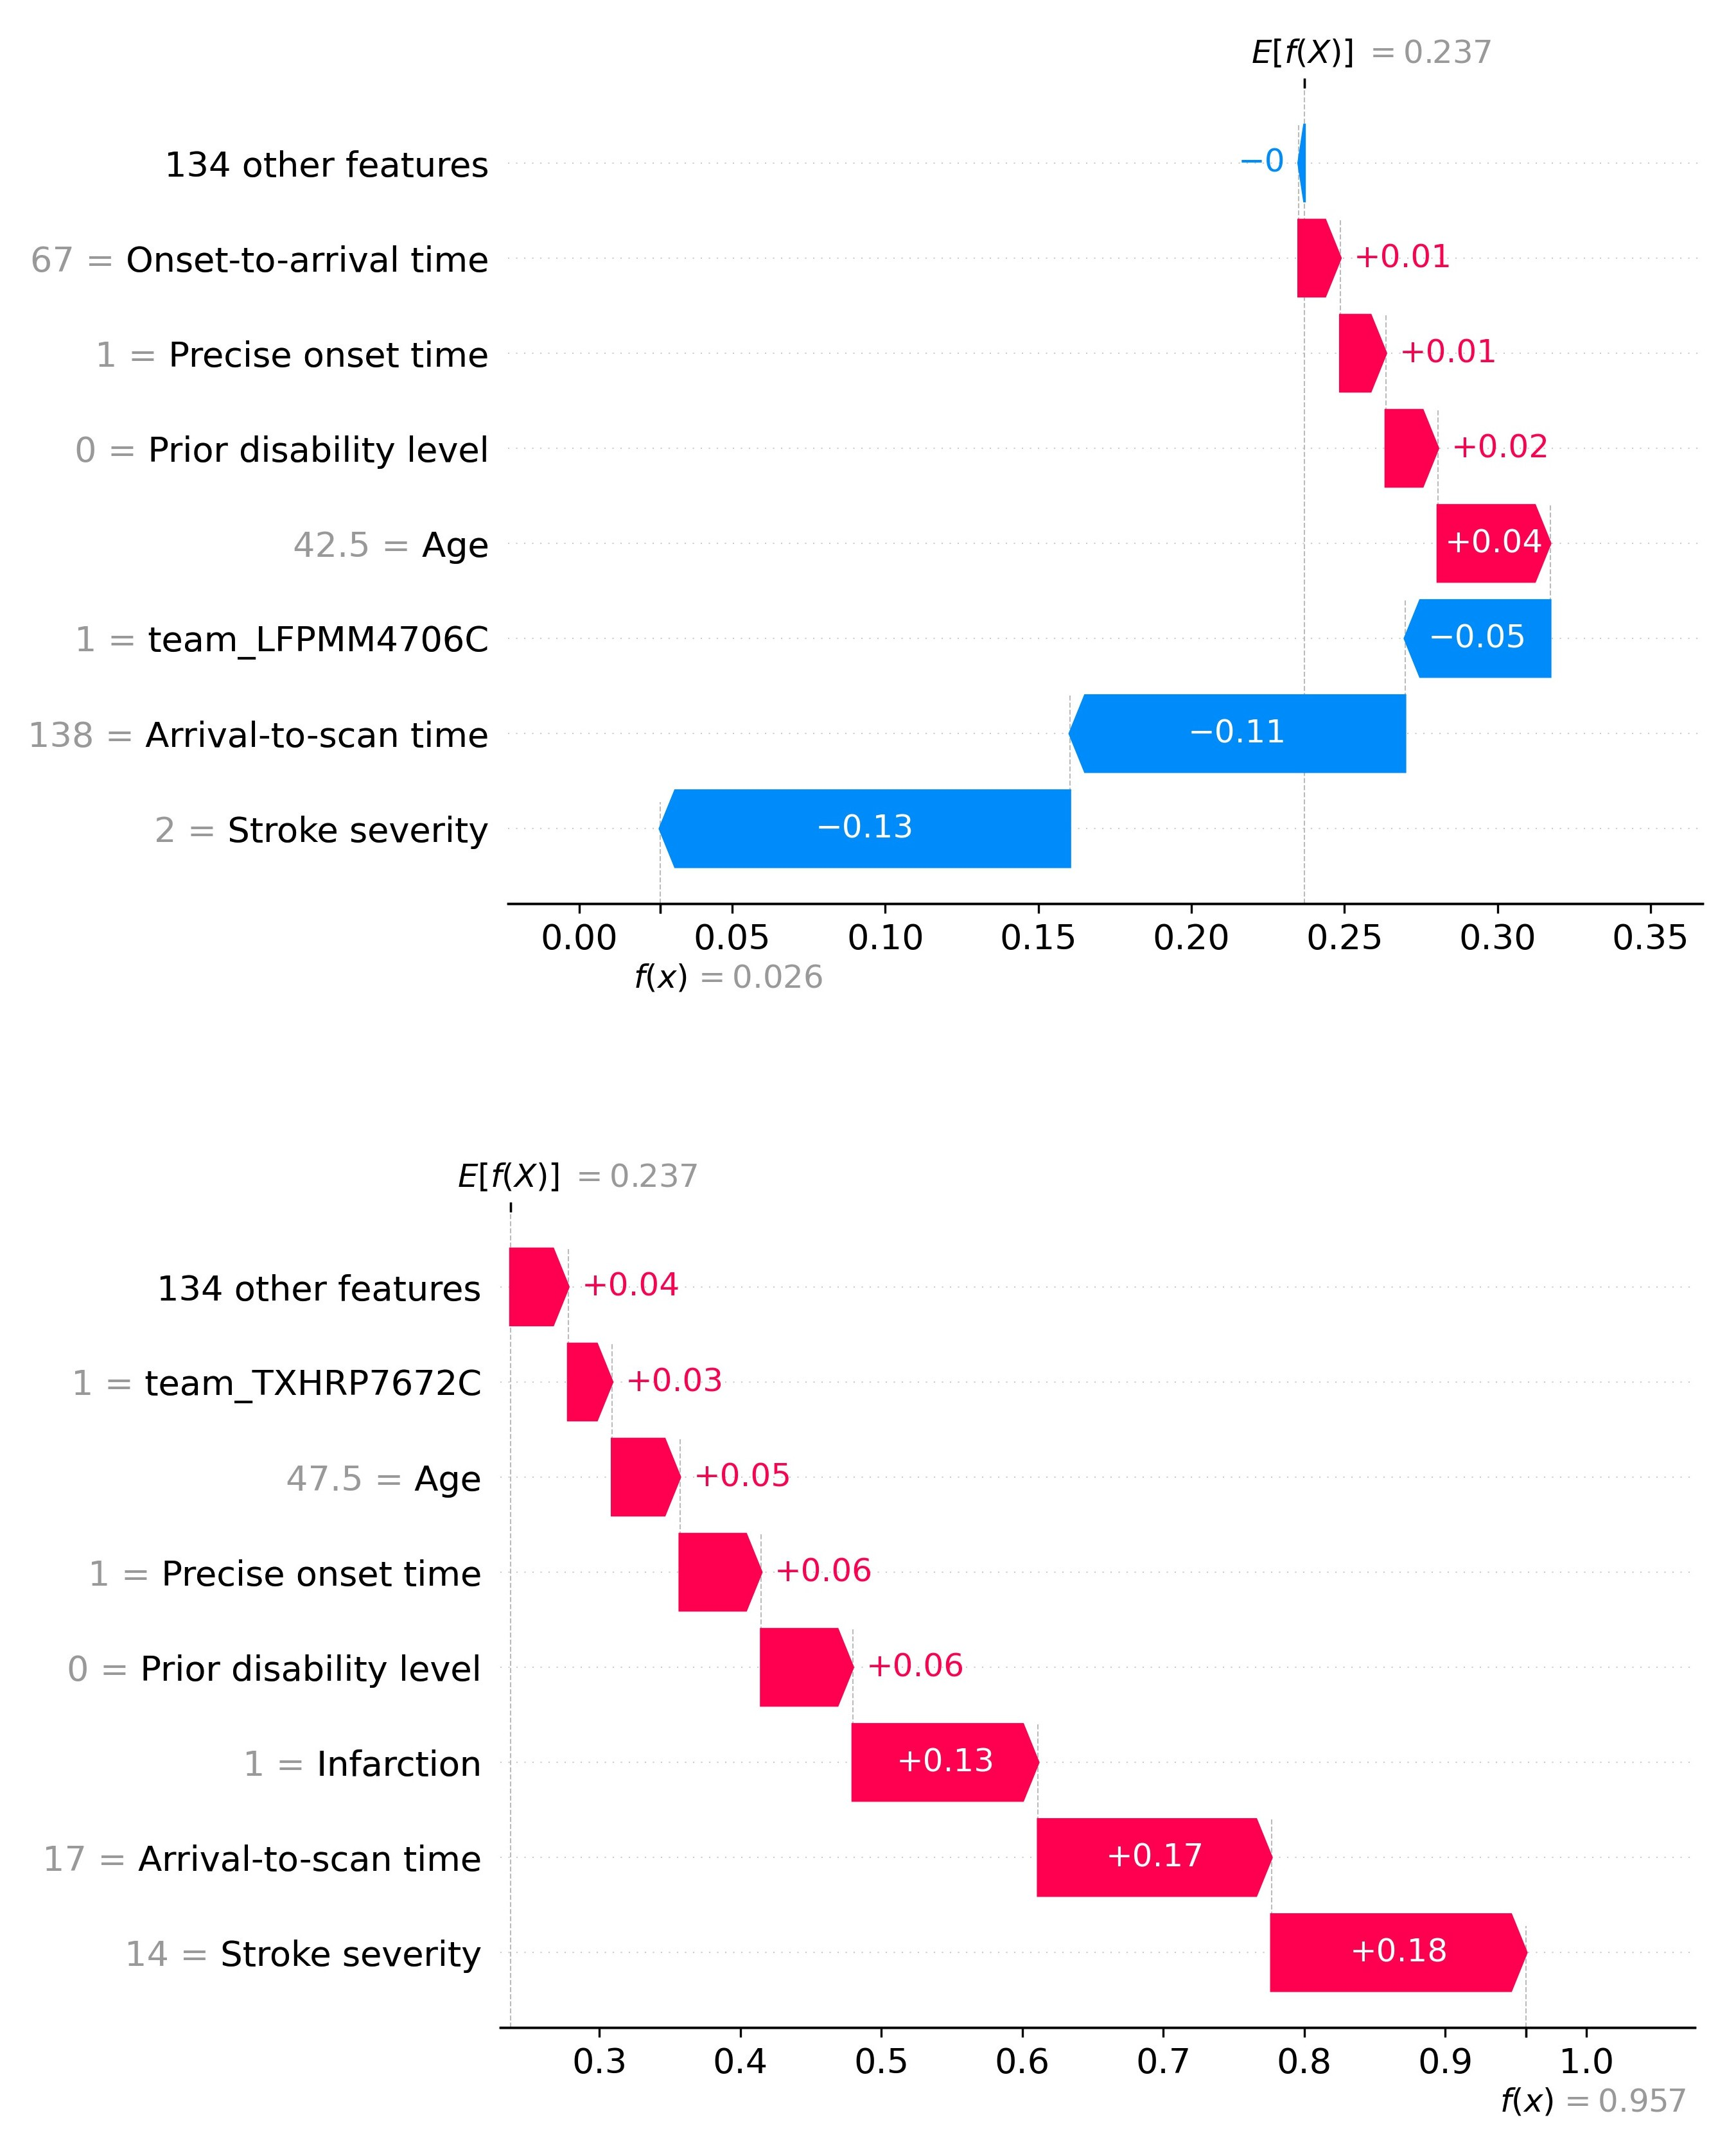
\includegraphics[width=0.6\textwidth]{./images/waterfall}
\caption{Waterfall plots showing the influence of each feature on the predicted probability of a single patient receiving thrombolysis. Top: An example of a patient with a low probability (2.6\%) of receiving thrombolysis. Bottom: An example of a patient with a high probability (95.7\%) of receiving thrombolysis.}
\label{fig:results_waterfall}
\end{figure}

%\newpage
%%%%%%%%%%%%%%%%%%%%%%%%%%%%%%%%%%%%%%%%%%%%%%%%%%%%%%%%%%%%%%%%%%%%%%%%

\subsection{The relationship between feature values and the odds of receiving thrombolysis}

Figure \ref{fig:shap_feature_subfigure} shows the relationship between patient level feature values and their SHAP values. Key observations are (with SHAP influence converted from log-odds to odds):

\begin{itemize}
    \item \emph{Stroke type}: The SHAP values for stroke type show that the model effectively eliminated any probability of receiving thrombolysis for non-ischaemic (haemorrhagic) stroke, with the odds of receiving thrombolysis fell by over 6,000 fold.
    \item \emph{Arrival-to-scan time}: The odds of receiving thrombolysis reduced by about 9 fold over the first 120 minutes of arrival to scan time.
    \item \emph{Stroke severity (NIHSS)}: The odds of receiving thrombolysis were lowest at NIHSS 0, increased and peaked at NIHSS 15-25, and then fell again with higher stroke severity (NIHSS above 25). The difference between minimum odds (at NIHSS 0) and maximum odds (at 15-25) of receiving thrombolysis was 25-30 fold.
    \item \emph{Stroke onset time type (precise vs. estimated)}: The odds of receiving thrombolysis were about 3 fold greater for precise onset time than estimated onset time.
    \item \emph{Disability level (mRS) before stroke}: The odds of receiving thrombolysis fell about 6 fold between mRS 0 and 5.
    \item \emph{Use of AF anticoagulants}: The odds of receiving thrombolysis were about 5 fold greater for no use.
    \item \emph{Onset-to-arrival time}: The odds of receiving thrombolysis were similar below 120 minutes, then fell about 3 fold between 120 and 240 minutes.
    \item \emph{Age}: The odds of receiving thrombolysis were similar below 80 years old, then fell about 2 fold between 80 and 110 years old.    
    \item \emph{Onset during sleep}: The odds of receiving thrombolysis were about 4 fold lower for onset during sleep.
    \item \emph{Hospital attended}: There was a 13 fold difference in odds of receiving thrombolysis between hospitals.
\end{itemize}

In summary the most thrombolysable patients have: an infarction stroke type; shorter arrival-to-scan times; moderate to severe stroke severity with NIHSS 10-25; a precise onset time; lower pre-stroke disability; were not taking anticoagulant medication; shorter onset-to-arrival times; were younger; did not have onset during sleep; attend a hospital with a high predisposition to use thrombolysis.
%\newpage

\begin{figure}%[!h]
\centering
\begin{subfigure}{.9\textwidth}
  \centering
    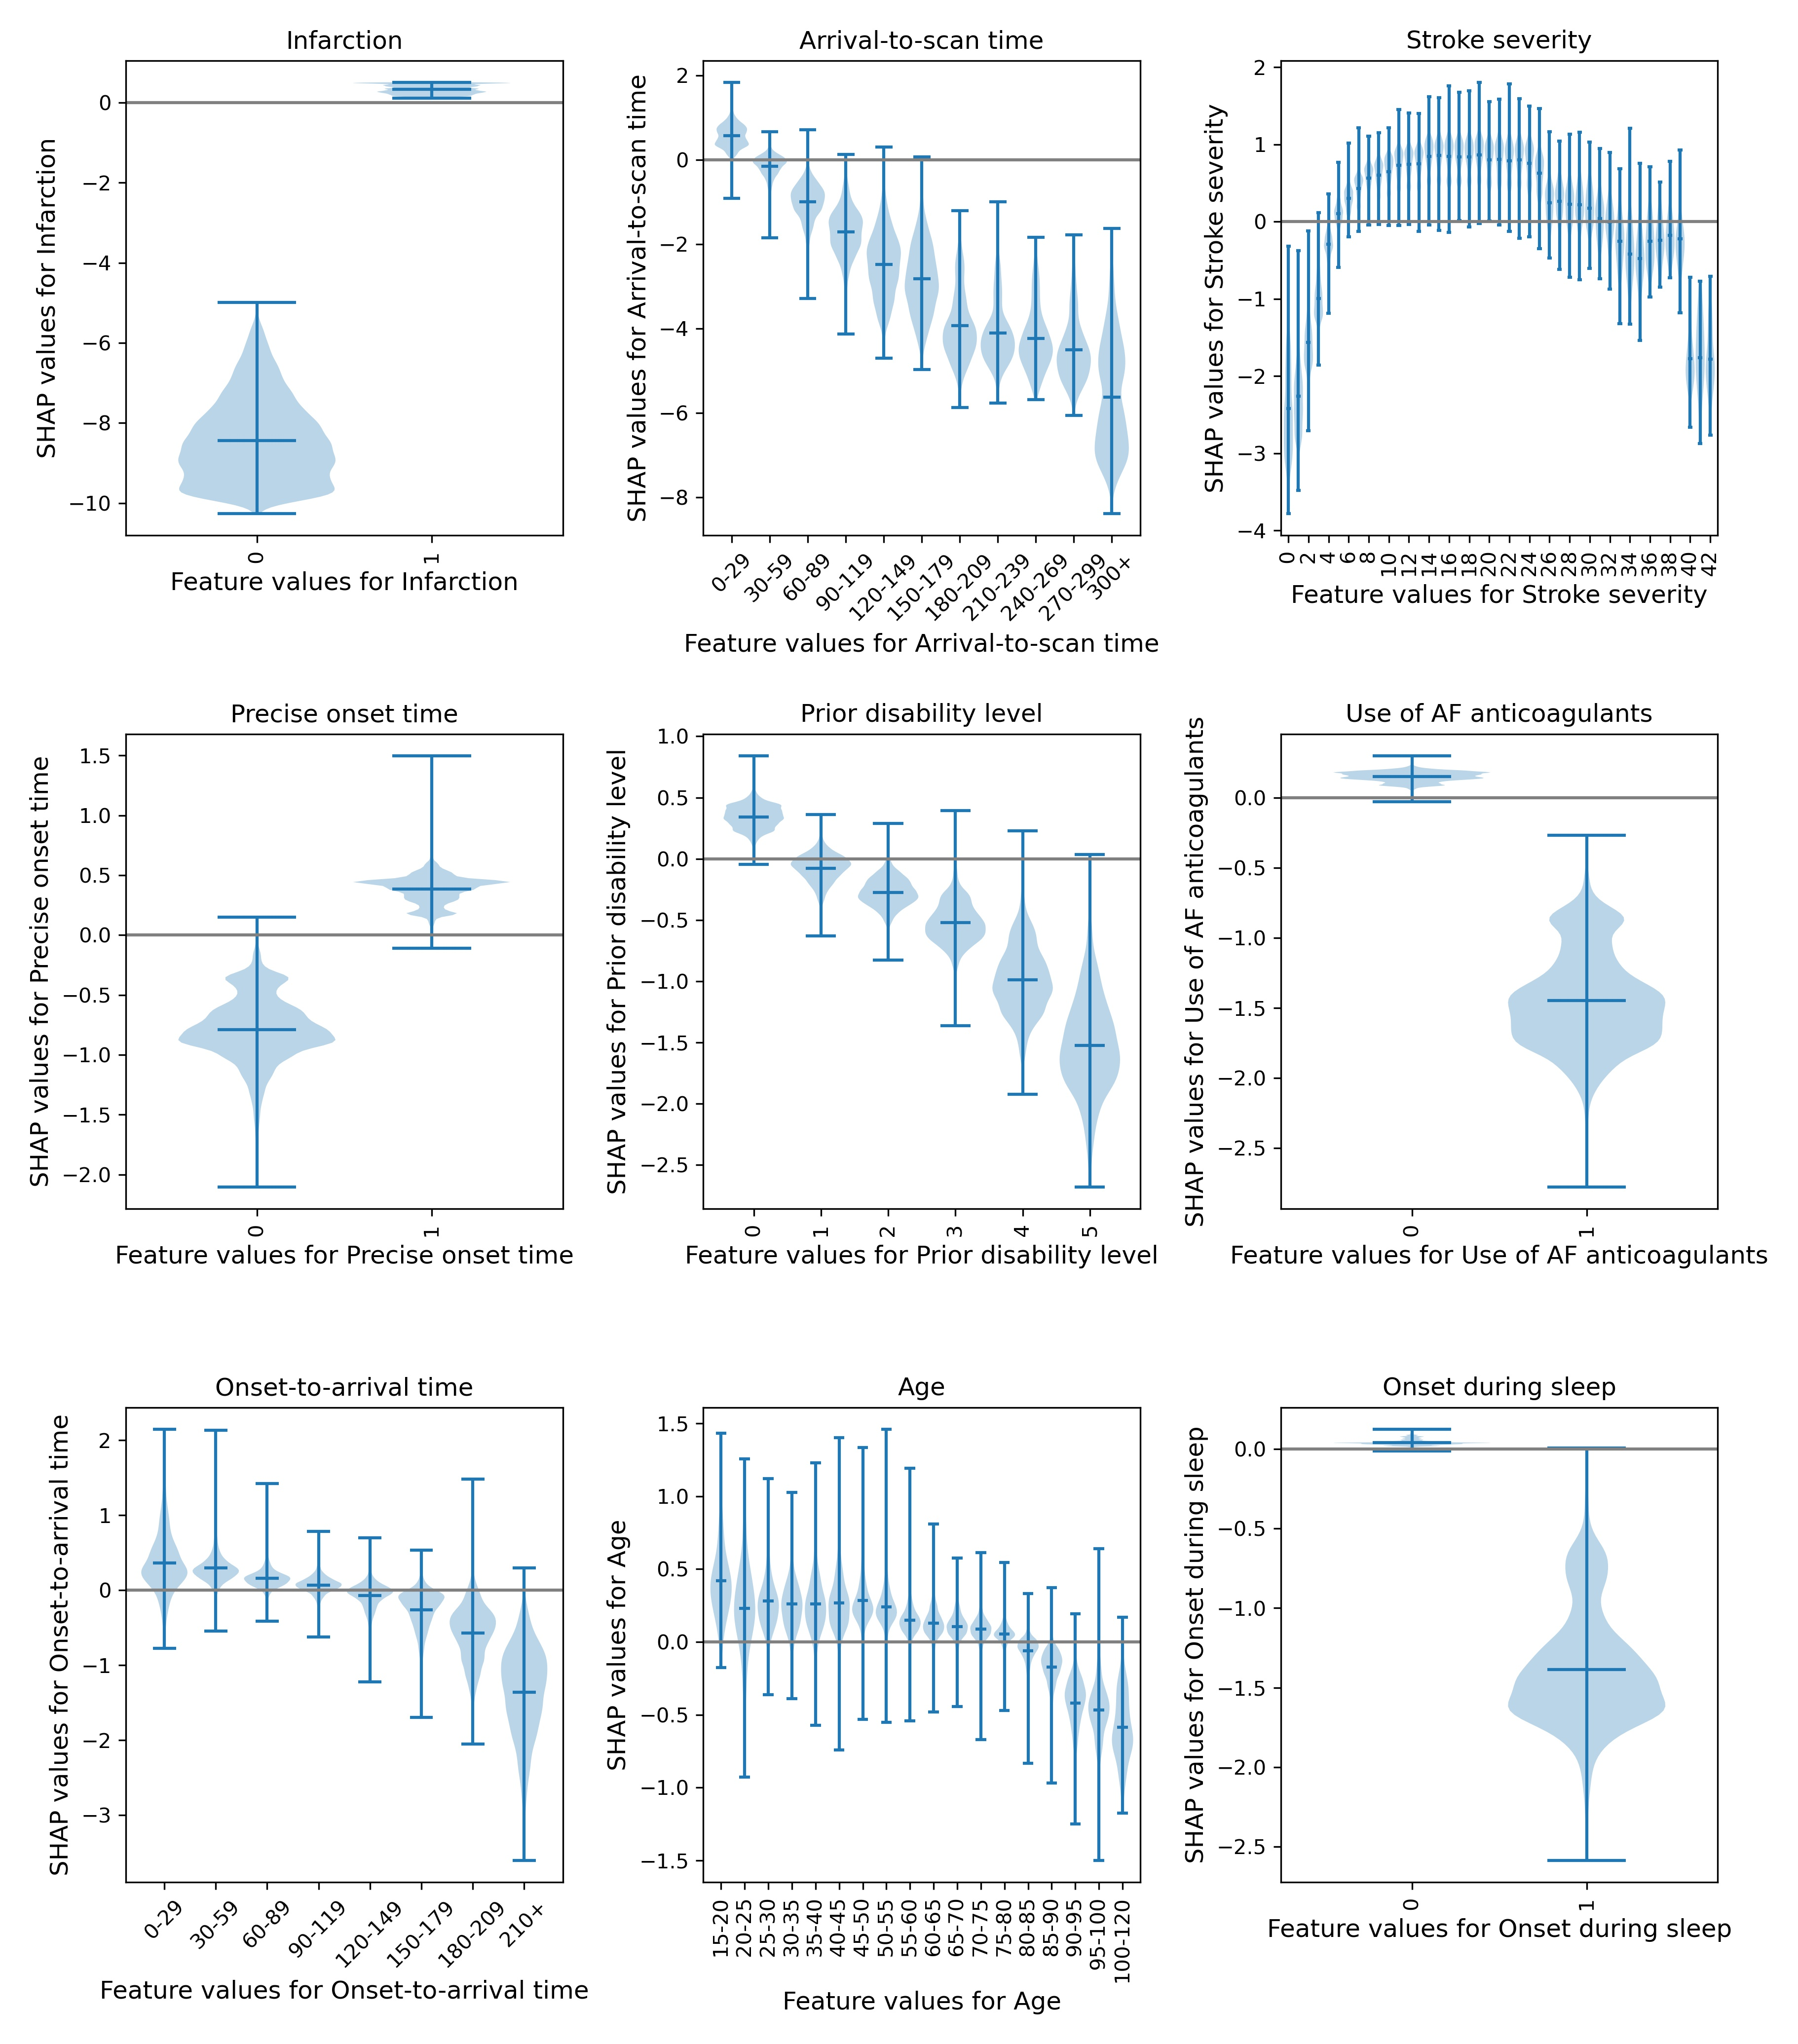
\includegraphics[width=1.\textwidth]{./images/03a_xgb_10_features_thrombolysis_shap_violin_all_features}
    \caption{}
  \label{fig:shap_feature_subfigure_a}
\end{subfigure}
\begin{subfigure}{.9\textwidth}
  \centering
    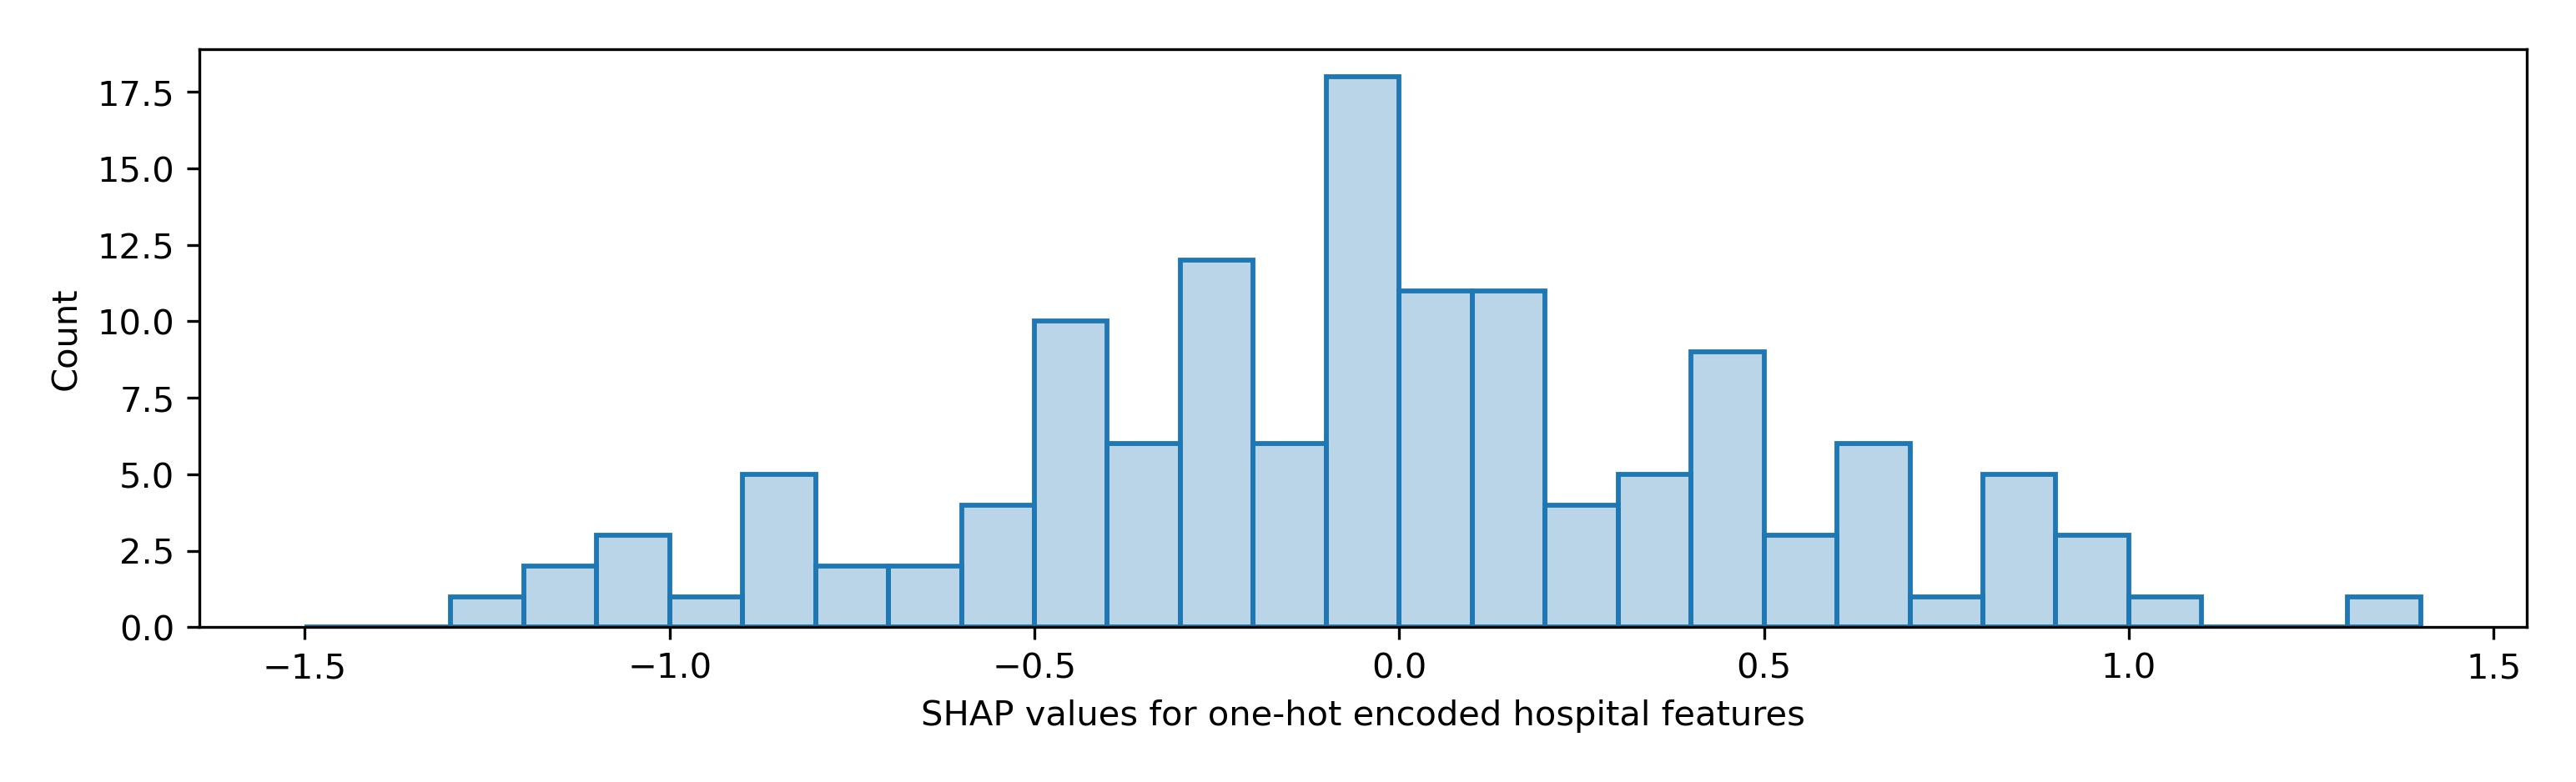
\includegraphics[width=1.\textwidth]{./images/03a_xgb_10_features_hosp_shap_hist}
    \caption{}
  \label{fig:shap_feature_subfigure_b}
\end{subfigure}
\caption{(a) Violin plots showing the relationship between SHAP values and feature values. The horizontal line shows the median SHAP value. The plots are ordered in ranked feature importance (using the mean absolute SHAP value across all instances) (b) Histogram showing the frequency of SHAP values for the one-hot encoded hospital feature.}
\label{fig:shap_feature_subfigure}
\end{figure}

%%%%%%%%%%%%%%%%%%%%%%%%%%%%%%%%%%%%%%%%%%%%%%%%%%%%%%%%%%%%%%%%%%%%%%%%
%\newpage
\subsection{How much of the between-hospital thrombolysis use can be explained by the identity of the hospital attended?}
%\subsection{How the hospital SHAP value compares with the hospitals use of thrombolysis}

The mean hospital attended SHAP value correlated with the observed hospital thrombolysis rate with an r-squared of 0.582 (figure \ref{fig:shap_correlation_subfigure_a}), suggesting that 58\% (P$<$0.0001) of the between-hospital variance in thrombolysis use may be explained by the attended hospitals' SHAP values, i.e. the hospitals' predisposition and/or preparedness to use thrombolysis. % KP DON'T THINK WANT THIS HERE NOW HAVE THE OTHER BELOW? By comparison, only four of the patient features had an r-squared greater than 0.1, P$<$0.0001 (infarction 0.448, arrival-to-scan time 0.273, anticoagulants 0.213, stroke severity 0.153), and with a maximum of 45\% of the between-hospital variance in thrombolysis use being explained by a single patient feature (infarction).

Using the \emph{10k holdout model}, the predicted use of thrombolysis across the 132 hospitals for the identical 10k cohort of patients (not used in training the model) ranged from 10\% to 45\%. The mean hospital attended SHAP value for the 10k cohort of patients correlated very closely with the predicted thrombolysis use in the 10k cohort of patients at each hospital, with an r-squared of 0.944 (figure \ref{fig:shap_correlation_subfigure_b}), confirming that the hospital attended SHAP is providing a direct insight into a hospitals' propensity to use thrombolysis.

%\iffalse
\begin{figure}[!h]
\centering
\begin{subfigure}{.49\textwidth}
  \centering
    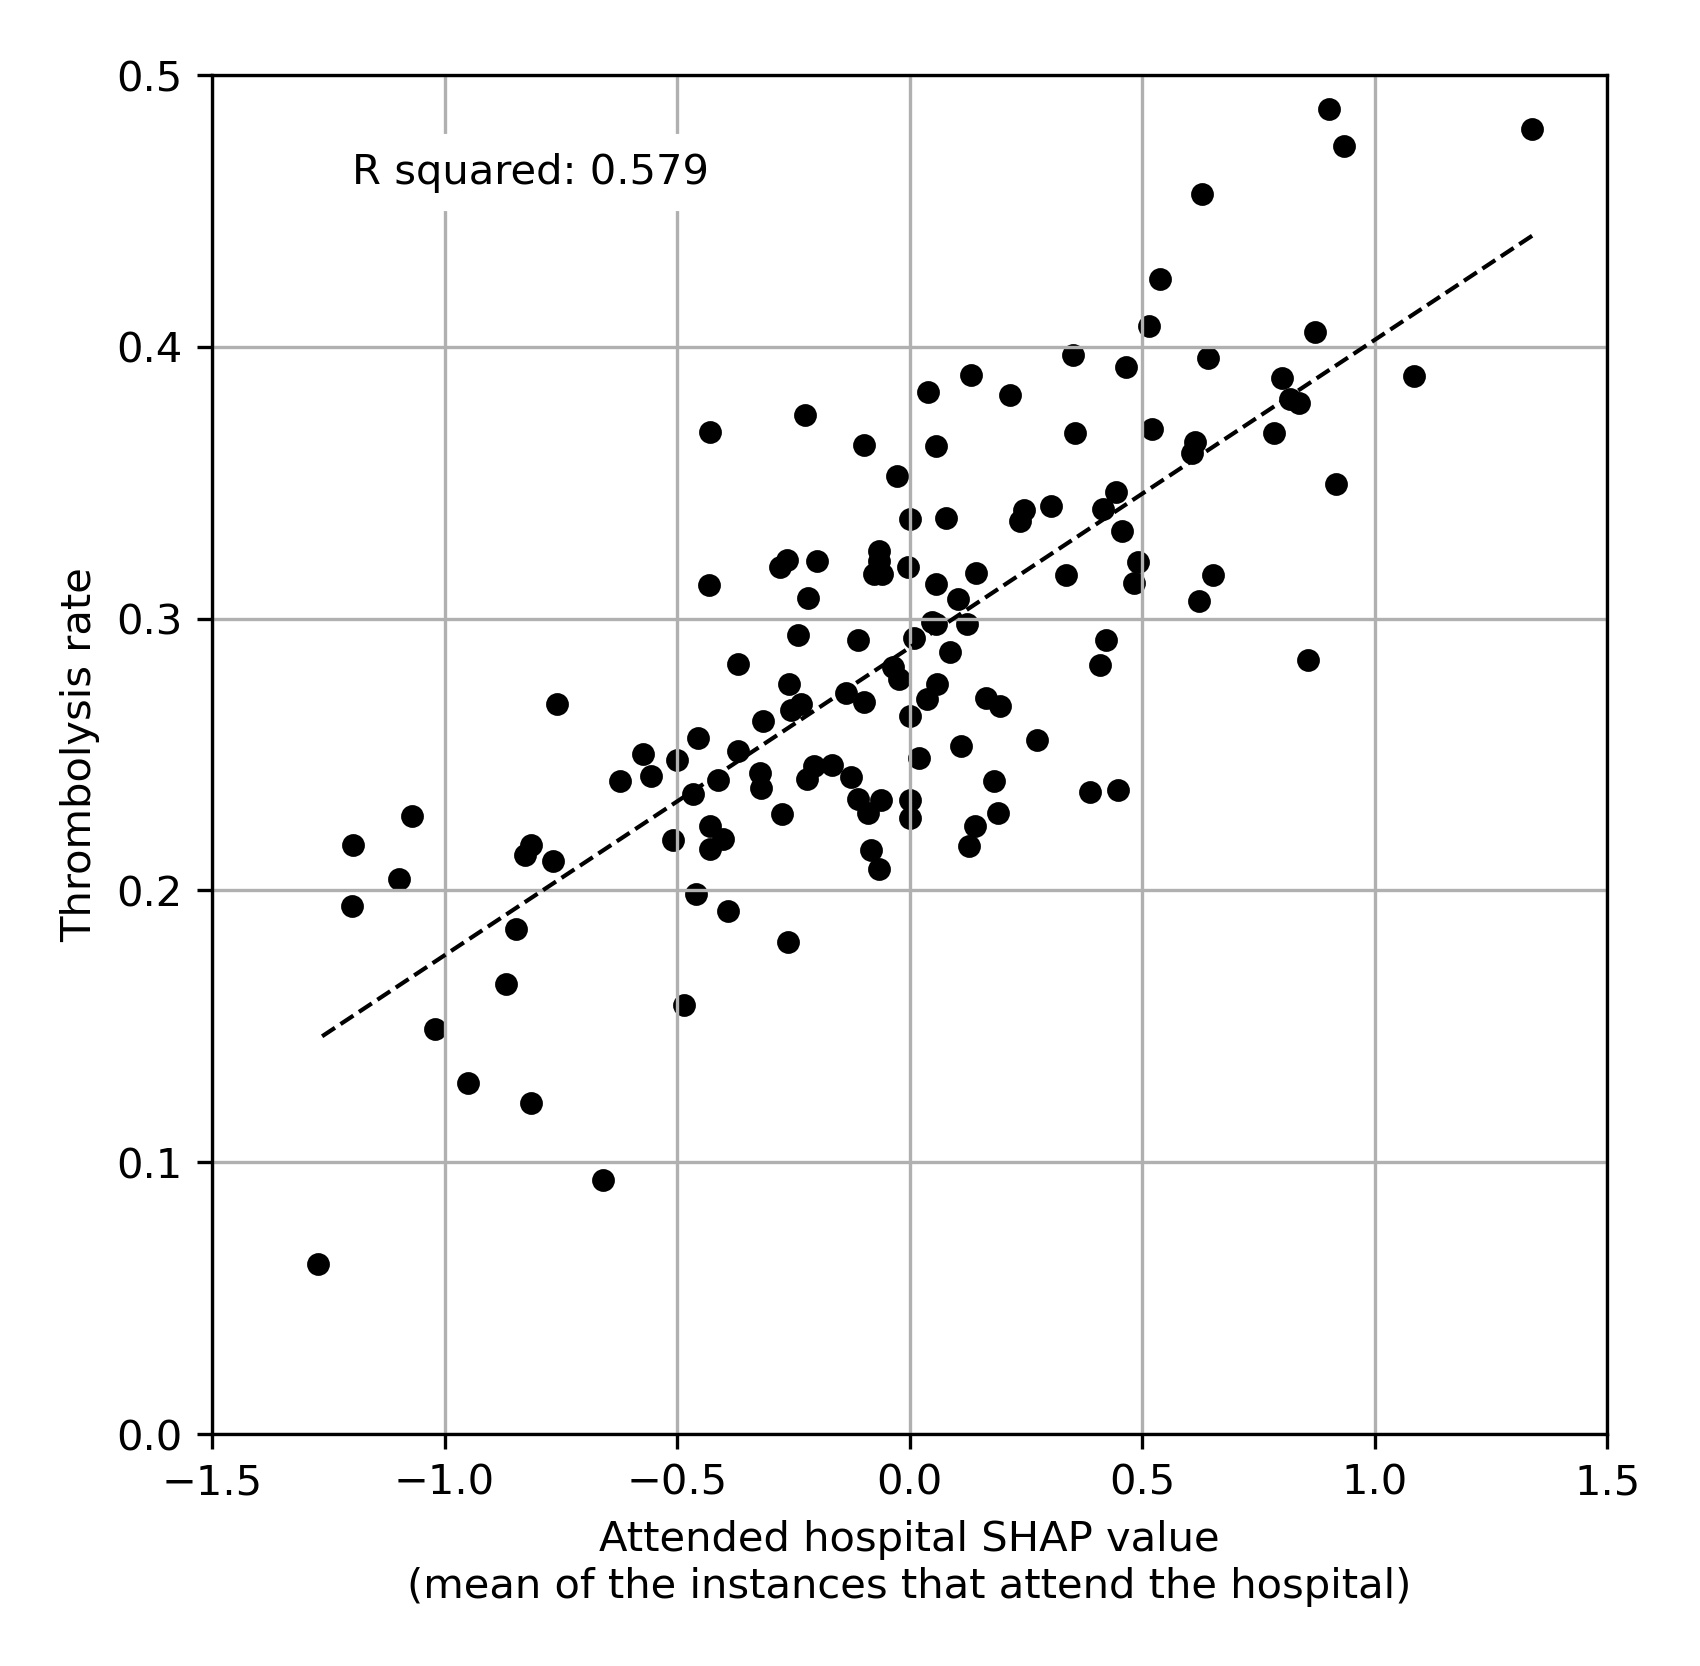
\includegraphics[width=0.9\textwidth]{./images/03b_xgb_10_features_attended_hosp_shap_vs_ivt_rate}
    \caption{}
  \label{fig:shap_correlation_subfigure_a}
\end{subfigure}
\begin{subfigure}{.49\textwidth}
  \centering
    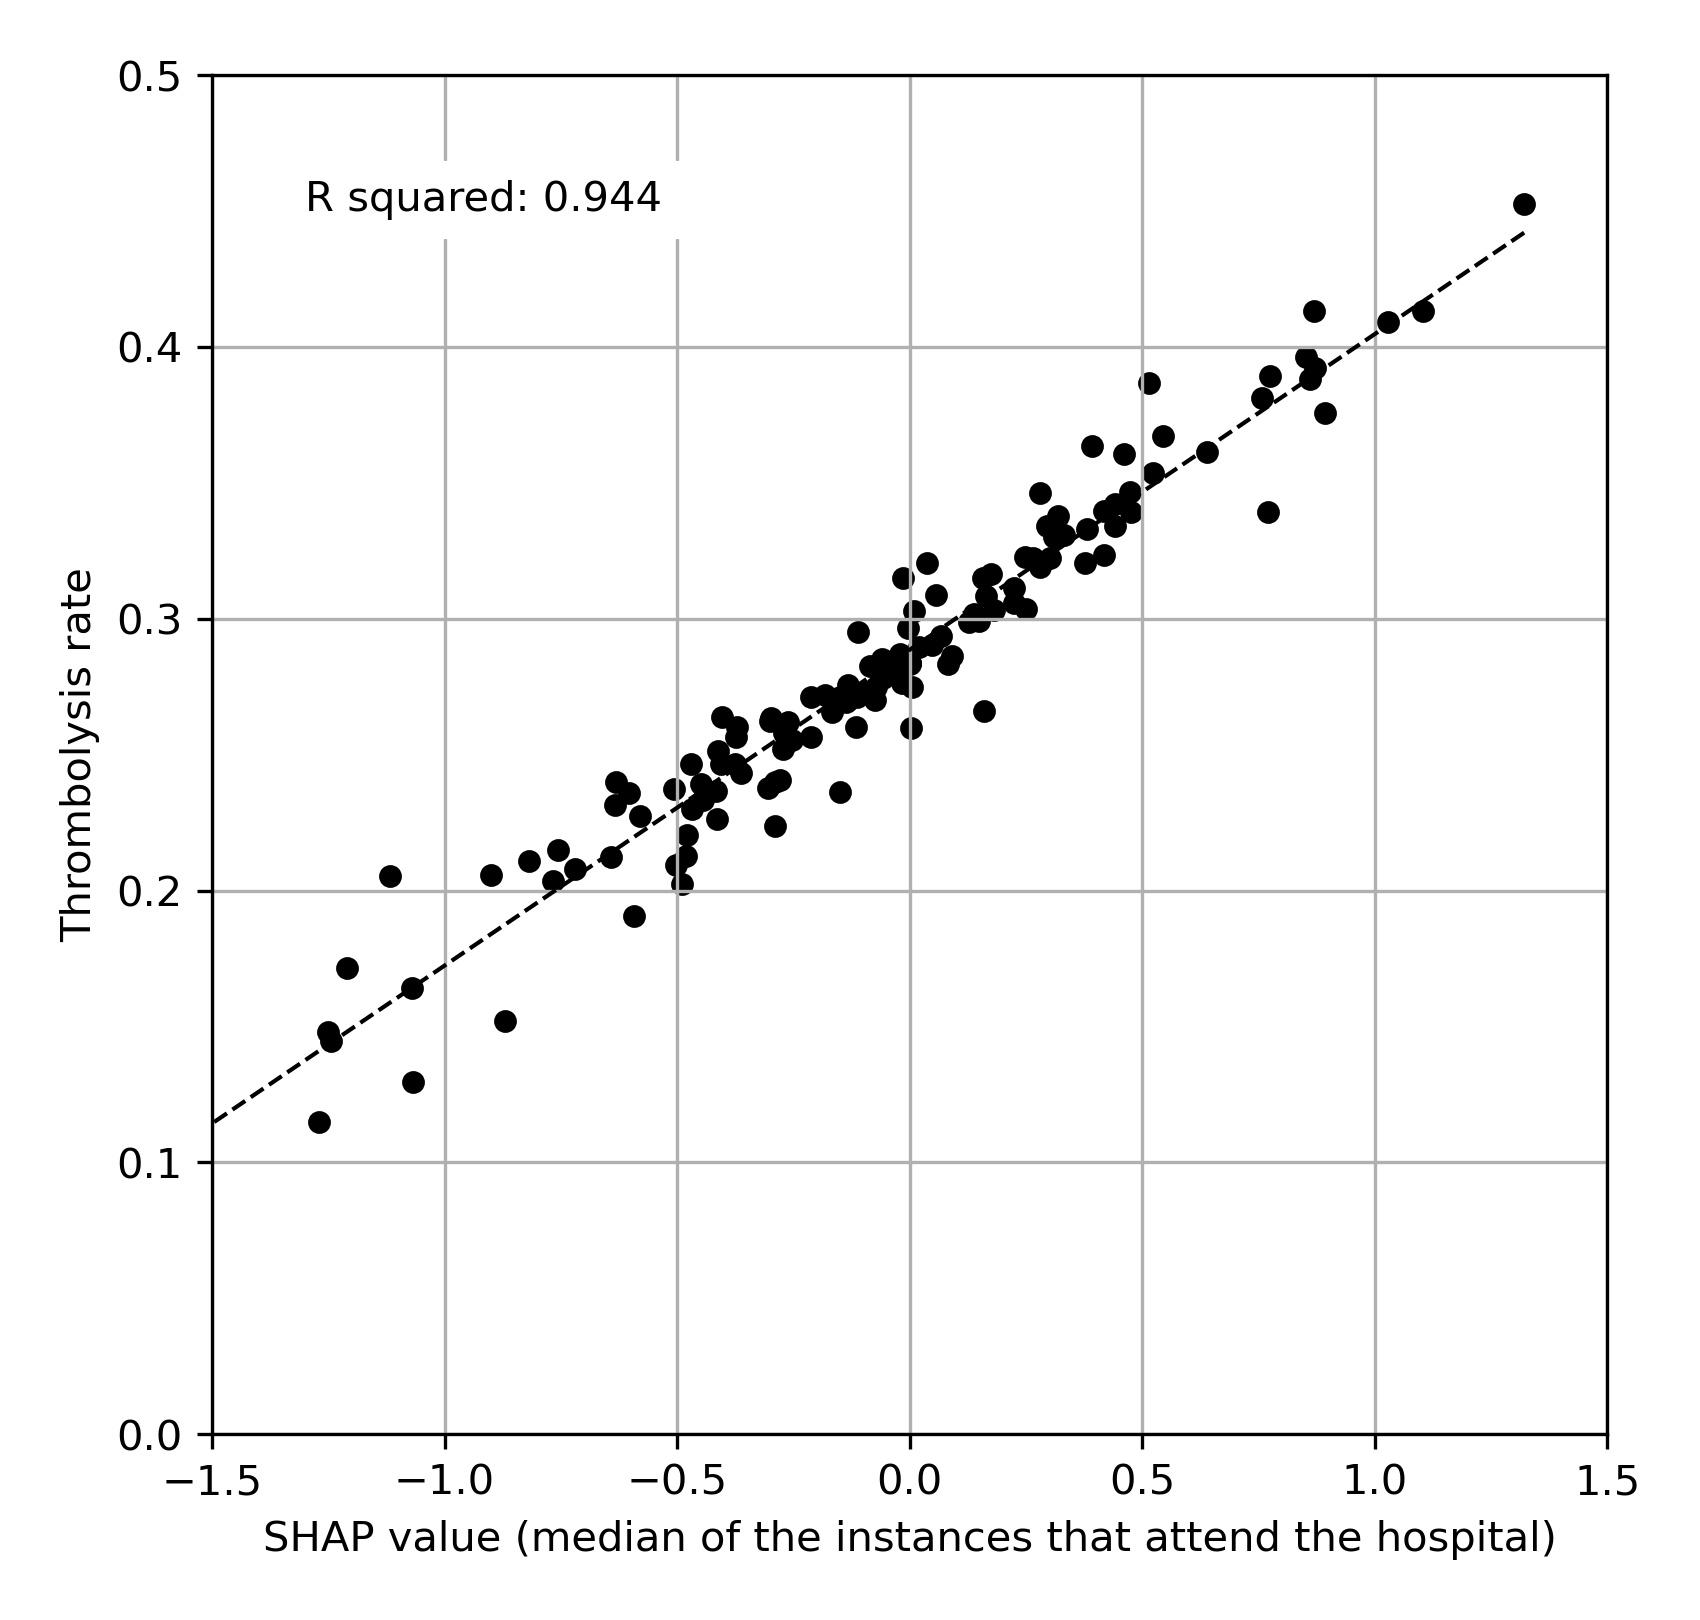
\includegraphics[width=0.9\textwidth]{./images/04_xgb_10_features_10k_cohort_attended_hosp_shap_value}
    \caption{}
  \label{fig:shap_correlation_subfigure_b}
\end{subfigure}
\caption{a) Correlation between mean hospital attended SHAP value and the observed thrombolysis use at each hospital (using the all data model). b) Correlation between mean hospital attended SHAP value and the predicted thrombolysis use at each hospital (using the 10k holdout model).}
%\label{fig:shap_correlation_subfigure}
\end{figure}
%%%%%%%%%%%%%%%%%%%%%%%%%%%%%%%%%%%%%%%%%%%%%%%%%%%%%%%%%%%%%%%%%%%
%\fi


%\newpage
\subsection{How much of the between-hospital thrombolysis use can be explained by the differences in the hospital identity and processes, and the differences in the patient populations?}%\subsection{How much of the hospitals use of thrombolysis can be explained by the differences in the hospital processes, and the differences in the patient mix}

We predicted thrombolysis use using mean SHAP values for patients attending each hospital. Figure \ref{fig:shap_multiple_regression} shows that 35\% (P$<$0.0001) of the variance in observed between-hospital thrombolysis use can be explained by the patient population, 72\% (P$<$0.0001) can be explained by hospital identity and processes, and that 94\% (P$<$0.0001) can be explained by the combined information from both the patient population and hospital identity and processes. 


\begin{figure}[!h]
    \centering
    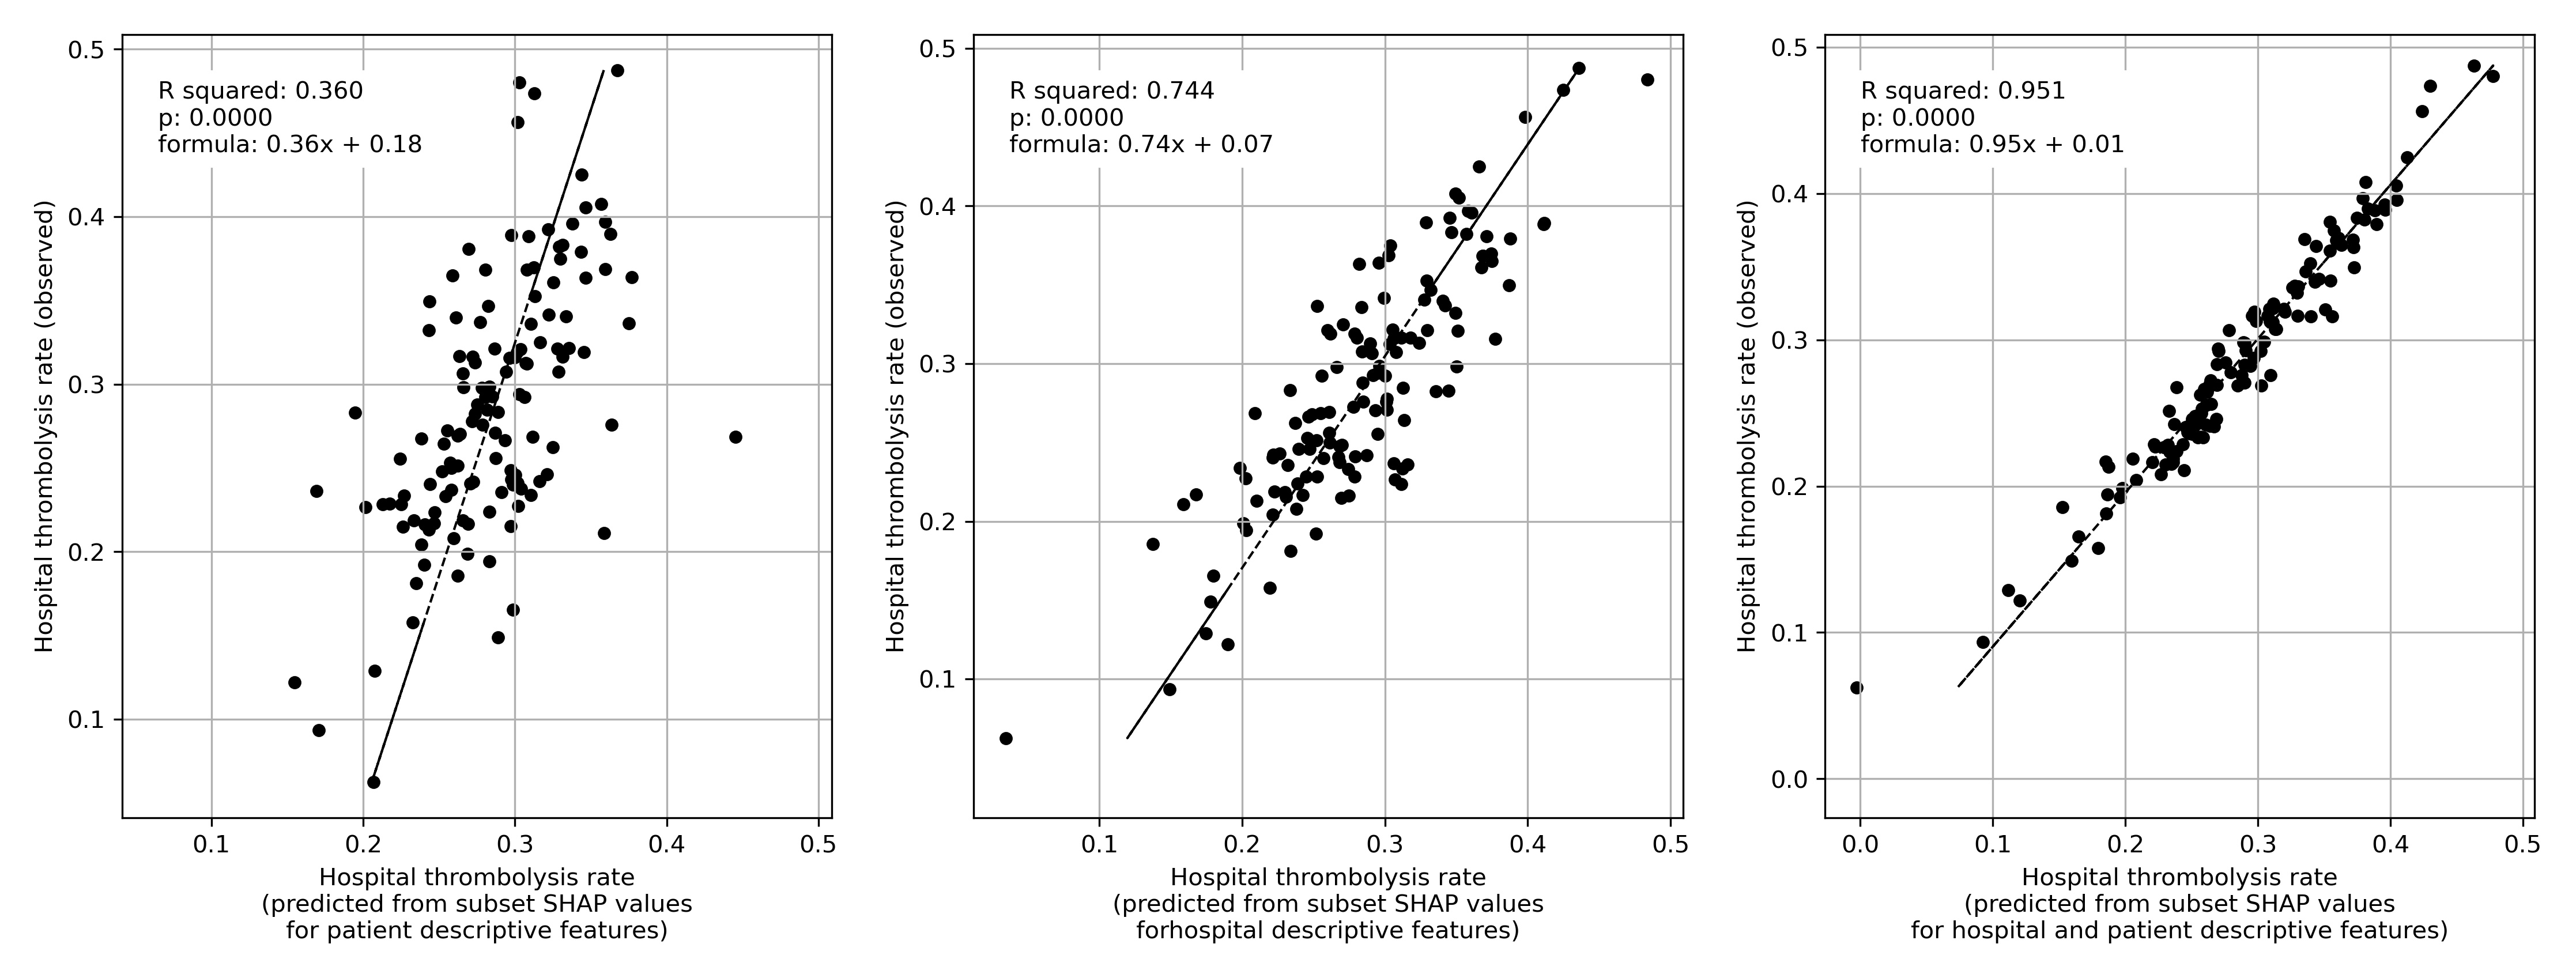
\includegraphics[width=0.9\textwidth]{./images/03f_xgb_10_features_multiple_regression_patient_hosptial}
    \caption{Multiple regression of subset SHAP values (mean of patients attending hospital) with hospital observed thrombolysis rate. LHS: Subset SHAP values for the eight patient descriptive features (age, stroke severity, prior disability, onset-to-arrival time, stroke type, type of onset time, anticoagulants, and onset during sleep). Middle: Subset SHAP values for the two hospital descriptive features (arrival-to-scan time, and hospital attended). RHS: Subset SHAP values for all 10 features (for both hospital and patient descriptive features).}
  \label{fig:shap_multiple_regression}
\end{figure}

%%%%%%%%%%%%%%%%%%%%%%%%%%%%%%%%%%%%%%%%%%%%%%%%%%%%%%%%%%%%%%%%%%%%%%%%
%\newpage
\subsection{Variation in hospital thrombolysis use for patient subgroups}

Figure \ref{fig:results_boxplot} shows boxplots of observed and predicted use of thrombolysis, broken down by patient subgroup. The nine subgroups of patients with one non-ideal feature (haemorrhagic stroke, arrival-to-scan time 60-90 mins, mild stroke severity, estimated stroke onset time, some pre-stroke disability, use of anticoagulants, onset-to-arrival time 150-180 mins, over 80 years old, and onset during sleep) all had reduced thrombolysis use than the complete patient population, and combining these non-ideal features reduced thrombolysis use further (illustrated by the patient subgroup with a mild stroke severity and an estimated stroke onset time). There was, however, significant variation between hospitals in use of thrombolysis in each of these subgroups. The observed and predicted thrombolysis use show the same general results, but some small differences existed: 1) The use of thrombolysis in \emph{ideal} patients is a little lower in the observed vs predicted results (mean hospital thrombolysis use = 89\% vs 99\%), 2) The predicted results show a stronger effect of combining non-ideal features, 3) The observed thrombolysis rate shows higher between-hospital variation than the predicted thrombolysis rate. This may be partly explained by the observed thrombolysis rate being based on different patients at each hospital, but may also be partly explained by actual use of thrombolysis being slightly more variable than predicted thrombolysis use (which will follow general hospital patterns, and will not include, for example, between-clinician variation at each hospital).

%Figure \ref{fig:results_boxplot} shows a boxplot of observed and predicted use of thrombolysis, broken down by patient subgroup. The nine subgroups of patients with one non-ideal feature (NIHSS $<$5, estimated stroke onset time, pre-stroke mRS $>2$) all had reduced thrombolysis use, and combining these non-ideal features reduced thrombolysis use further. The observed and predicted thrombolysis use show the same general results, but some small differences existed: 1) The use of thrombolysis in \emph{ideal} patients is a little lower in the observed vs predicted results (mean hospital thrombolysis use = 89\% vs 99\%), 2) The predicted results show a stronger effect of combining non-ideal features, 3) The observed thrombolysis rate shows higher between-hospital variation than the predicted thrombolysis rate. This may be partly explained by the observed thrombolysis rate being based on different patients at each hospital, but may also be partly explained by actual use of thrombolysis being slightly more variable than predicted thrombolysis use (which will follow general hospital patterns, and will not include, for example, between-clinician variation at each hospital).

%For both the observed and predicted thrombolysis, subgroup thrombolysis use tended to reduce in parallel (r-squared 0.221 to 0.308 in observed thrombolysis use, and 0.445 to 0.621 in the predicted thrombolysis use). \kpFIXME{NEED TO CALCULATE NEW VALUES IF INCLUDING, BUT NO GRAPH TO SHOW THIS, IN APPENDIX}

\begin{figure}[!h]
\centering
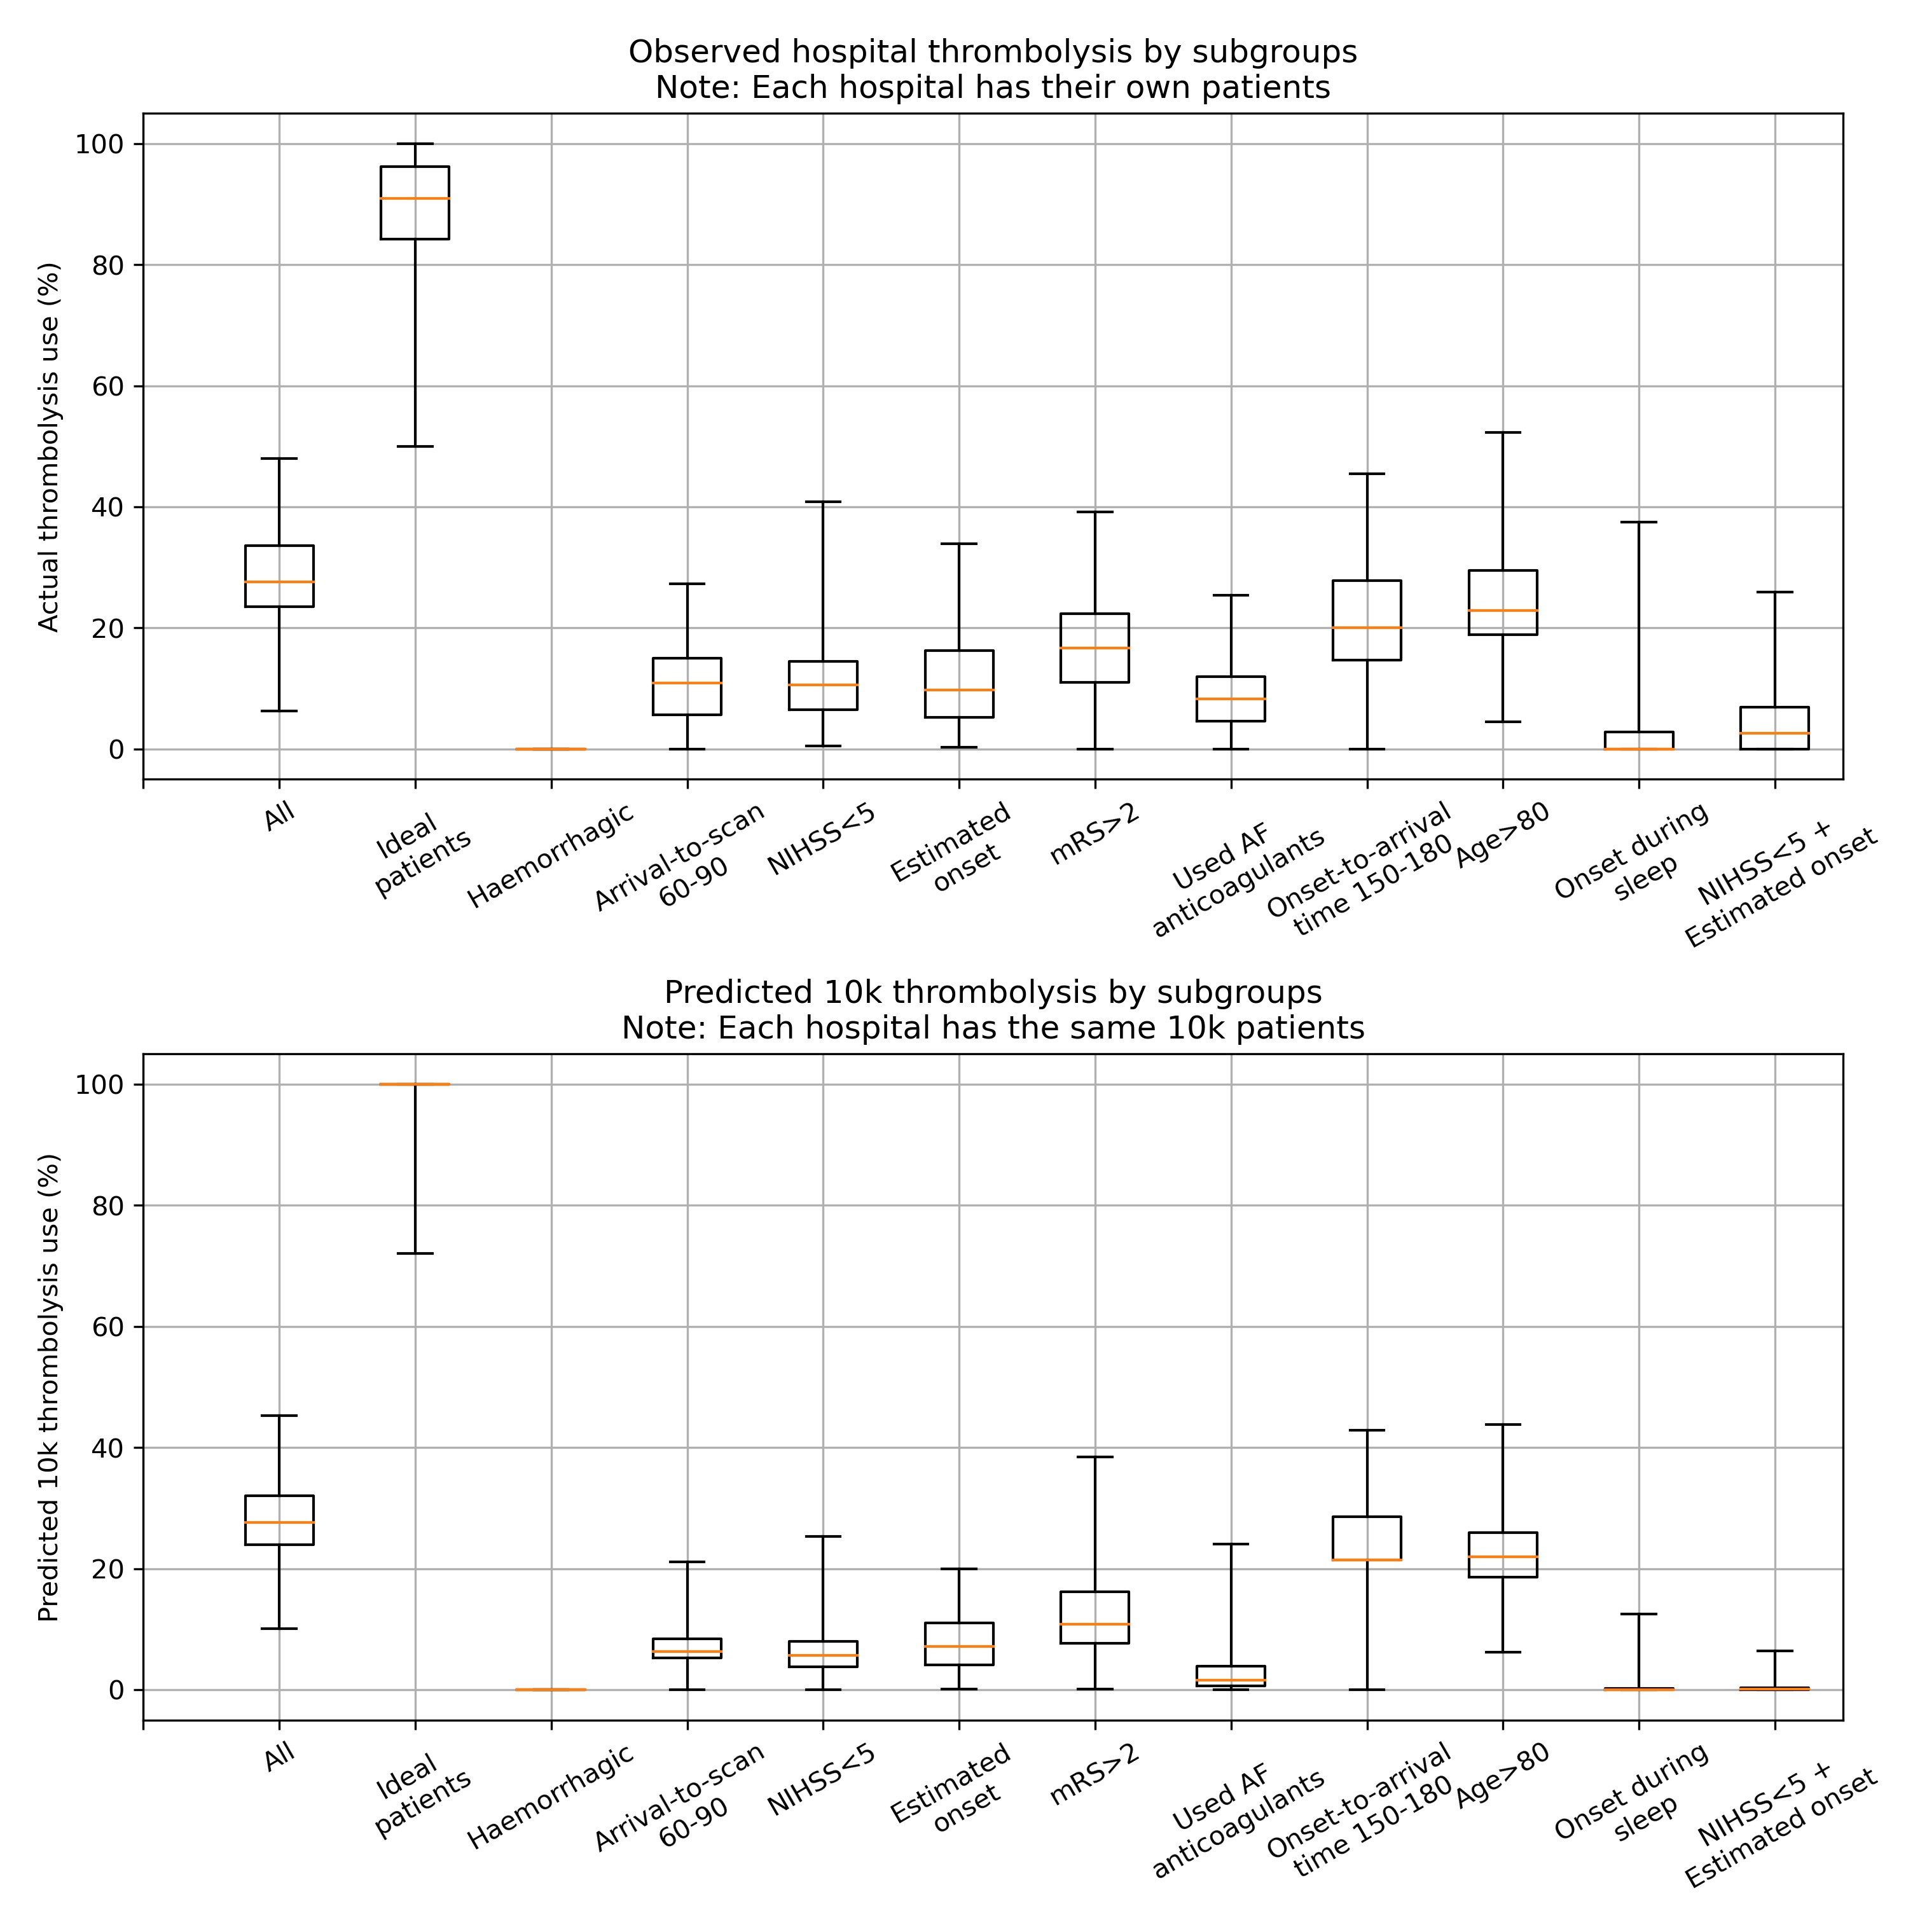
\includegraphics[width=1\textwidth]{./images/15a_xgb_10_features_10k_cohort_actual_vs_modelled_subgroup_boxplot}
%{./images/15a_actual_vs_modelled_subgroup_violin}
\caption{Boxplot for either observed (top) or predicted (bottom) use of thrombolysis for subgroups of patients. The `ideal patients' subgroup has a mid-level stroke severity (NIHSS in range 10-25), short arrival-to-scan time (less than 30 minutes), stroke caused by infarction, precise stroke onset time known, no pre-stroke disability (mRS 0), not taking any atrial fibrillation anticoagulants, short onset-to-arrival time (less than 90 minutes), younger than 80 years old, and onset not during sleep. The single features are ordered in ranked feature importance (using the mean absolute SHAP value across all instances). }
\label{fig:results_boxplot}
\end{figure}
\newpage






\section{Discussion}

We have built on our previous work to predict thrombolysis use from patient characteristics, by creating an \emph{explainable machine learning model} which maintains the high accuracy that we previously achieved (85\%). The model was well-calibrated, with the average predicted probability of thrombolysis for any group of patients matching the proportion of those patients who did receive thrombolysis. The SSNAP registry data used therefore appears to contain most of the information used to make thrombolysis decisions in clinical practice. To further support this, when we identified a group of patients that the model predicts would receive thrombolysis all the time in the large majority of hospitals, the observed thrombolysis rate of that group was 90\% in half the hospitals}.

We have not designed our model to indicate whether an individual patient \emph{should} receive thrombolysis. Despite our high accuracy, there will be relevant patient details not known to us that would preclude use of thrombolysis. Rather we have used machine learning to determine the usual patterns of use of thrombolysis that are common across hospitals, and vary between hospitals. These learned patterns help identify and show effects of varying patient characteristics.

In general, using SHAP values to uncover the relationship between patient characteristics and the probability of receiving thrombolysis, we found that the probability of receiving thrombolysis fell with increasing arrival-to-scan times, was dependent on stroke severity with the probability of receiving thrombolysis being highest between NIHSS 10 and 25, was lower when onset time was estimated rather than known precisely, and fell sharply with increasing disability prior to stroke. These patterns are similar to the observations of a discrete choice experiment with hypothetical patients \cite{de_brun_factors_2018}, but in our study we confirm these patterns in actual use of thrombolysis, can be quantitative about the effect, and we add the importance of time-to-scan and whether an onset time is known precisely. Using SHAP we can identify the general effect of each patient characteristic, such as stroke severity, and then also whether individual hospitals are influenced to a greater or lesser extent by that characteristic.

Hospital SHAP values correlated very closely with the predicted use of thrombolysis in a 10k cohort of patients, confirming that the hospital SHAP value provides a measure of the predisposition of a hospital to use thrombolysis. We found that hospital processes explained 74\% of the variance in observed thrombolysis, suggesting that clinical decision-making around thrombolysis accounts for the majority of variance in use of thrombolysis between hospitals for those patients who arrive at hospital within 4 hours of known (precise or estimated) stroke onset time. 

\kpFIXME{NEED TO EDIT THIS PARAGRAPH TO REFLECT NEW SUBGROUP ANALYSIS. LISTS AND EXPLAINS THE 3 FEATURES THAT WERE INCLUDED, NOW HAVE ALL FEATURES INCLUDED, AND GOING TO CHOOSE 1 COMBO SUBGROUP}
After observing the general patterns that exist in the use of thrombolysis, we created a subgroup of patients reflecting what appeared to be an \emph{ideal} candidate for thrombolysis, and also a subgroup per feature where we expected to see lower use of thrombolysis (low stroke severity, no precise onset time, pre-stroke disability, older age, longer arrival to scan, haemorrhage, using anticoagulants, longer onset to arrival, and onset during sleep). Observed thrombolysis in these groups reflected the patterns identified by the SHAP analysis. For the \emph{ideal} candidates of thrombolysis, half of stroke units would give thrombolysis to at least 90\% of these patients, but some units gave it to significantly fewer patients. Use of thrombolysis in the other subgroups of patients was, as expected, lower, but use also varied significantly, with use ranging between 0\% and \kpFIXME{DOES 40\% STILL HOLD HERE? Onset to arrival has a range that incorporates 100\%?} 40\% for these less ideal patients. These patterns, both of average use, but also range of use between hospitals, were repeated with expected use of thrombolysis in the same 10k patient cohort of patients.

\iffalse
REFERS TO ARTIFICIAL PATIENTS THAT MAY NOT INCLUDE
Another way of showing variation between units was to use artificial patients. After observing the general patterns that exist in the use of thrombolysis, we created an artificial patient representing an \emph{ideal} candidate for thrombolysis that was predicted to receive thrombolysis at almost every hospital. But when we reduced their stroke severity and attributed an estimated onset time the predicted use of thrombolysis dropped to 35\% of hospitals. With the use of SHAP values it is possible to take the next step into understanding this result by peering into how each hospital responds to the characteristics of this patient, to elucidate where hospitals vary in their attitudes to thrombolysis.
\fi

This novel tool examines and understands between-hospital variation in clinical decision making in the acute stroke setting. The application of this tool is not restricted to stroke, or to England and Wales. It can be applied to any clinical decision where there is routinely collected data that quantifies the patients pathway up to the point of the decision, and the features recorded represent a sufficient quantity of the information that clinicians use to make their decision.

The use of mega-datasets such as SSNAP to understand sources of variation in clinical practice between large number of acute stroke centres across the UK presents a unique opportunity to understand the specific influences behind the significant residual between-hospital variation in thrombolysis use.  In particular, it allows national quality improvement projects such as SSNAP to counter one of the most common objections raised to comparative audit: that the patients presenting to any one particular site are in some way unique, thereby accounting for most of the variation in clinical quality between that site and all the others – what, informly, has been termed the `special hospital fallacy'. Although the patient-mix does vary between hospitals, and will contribute to the thrombolysis use achievable by an individual hospital (being able to explain 34\% of the variance in between-hospital thrombolysis use, and our previous work identifying the need for individual hospital thrombolysis rate targets of between n and n\%), the majority (74\%) of between-hospital variation can be explained by hospital-level rather than patient-level factors. Another strength of the dataset is its richness. When the observed thrombolysis rate at each hospital is compared to the predicted thrombolysis rate, less than 3\% residual variation remains – suggesting that no more than 3\% of variation in thrombolysis use can be accounted for by factors that are not already measured in the national registry. SSNAP appears to contain the data that is needed for thrombolysis decisions. A far greater proportion of variation in clinical practice is accounted for by the hospital/team’s own approach to non-ideal features in patients presenting with acute ischaemic stroke – principally stroke severity (a disposition to avoid thrombolysis in patients outside the NIHSS range 10-25), an estimated rather than a precisely-reported onset time (an inclination to avoid thrombolysis unless all the timings are precisely known), and pre-stroke disability (a tendency to avoid thrombolysis in patients already needing at least the help of another person with ordinary daily activities). It is disappointing that even though this disability-saving treatment was first licensed for approval for use over 20 years ago, it is still subject to such large 7-fold variation in clinical judgement or opinion regarding the selection of patients most appropriate for use. In our previous work \cite{allen_using_2022}, we have shown that increasing the uptake of thrombolysis through the administration of treatment to more patients and sooner after stroke, offers the prospect of more than doubling the proportion of patients after stroke who are left with little or no disability (mRS 0 or 1). At a time when there is an appropriate focus of effort on expanding the use of endovascular therapy in acute ischaemic stroke, it is sobering to consider how much population benefit there still remains to accrue from the fullest possible implementation of a cheaper technology that has been available for over 20 years. Far greater scrutiny of such residual variation in clinical practice is clearly warranted, given the extent to which it appears to be acting as a barrier to successful implementation. Recent studies have highlighted that clinicians can be reluctant to modify their behaviour in response to audit and feedback when it is not seen to be clinically meaningful, recent or reliable \cite{bekker_give_2022}, so the full potential of audit and feedback is not realised \cite{foy_revitalising_2020} despite the evidence of a beneficial effect especially when baseline performance is low \cite{ivers_audit_2012}. The development of bespoke, individualised feedback (at least at hospital level) based on actual and recent activity may increase the impact of efforts at data-driven quality improvement targeted at increasing overall uptake of thrombolysis through reducing variation.

%EXTRA DISCUSSION WORDS
%We have shown a novel tool to examine and understand between-hospital variation in clinical decision making in the actue stroke setting. The application of this tool is not restricted to stroke, or the UK. It can be applied to any clinical decision where there is routinely collected data that quantifies the patients pathway up to the point of the decision, and represents a sufficient quantity of the information that the clinicians use.

%Strength: Diversity of patients, dataset size
%Moving on from previous work, improved models explanability whilst maintaining model accuracy.

\subsection{Limitations}

This machine learning study is necessarily limited to data collected for the national stroke audit. Though we have high accuracy, and can identify clear patterns of use of thrombolysis, the data will not be sufficient to provide a decision-support tool. Nor is it a causal model. We may also be missing information that could otherwise have improved the accuracy still further. We also necessarily analyse thrombolysis at hospital level rather than at the level of the individual clinician. The model has high accuracy and can identify clear patterns, suggesting the capability to identify and characterise a centre's culture in the use of thrombolysis, but we do not identify variation in thrombolysis between individual clinicians in the same hospital.

SHAP is a popular method for explaining the output of machine learning models, but it does have some limitations. SHAP values are an approximation of the Shapley values, from which they are based, in order to calculate them efficiently. Even so, SHAP can be computationally expensive and slow for large datasets and complex models. SHAP can only help to explain the fitted model, and so it can only as good as the model (with caveats around training data containing bias, or incomplete information). Another limitation is the interpretation of SHAP values and its components (the main effect and interactions) can be challenging. To aid our dissemination of the findings from SHAP we have engaged with clinicians, patients and carers to learn how best to communicate this information. SHAP assumes that each feature's contribution is independent of the presence or absence of other features as SHAP values may not accurately capture the true contribution of each feature to the model output if feature independence is not held. We ensured that very little covariance existed between the 10 features that were included in the models. %To address this limitation for models where this is not possible, researchers are exploring new methods that can better capture feature interactions and dependencies, such as integrated gradients and DeepLIFT.

We acknowledge that not all countries have a national stroke audit dataset, however we hope that this paper helps to demonstrate what type of analysis can be done should resources be allocated to collect their national data.

\section{References}
\bibliographystyle{naturemag}
%\bibliographystyle{plainnat}
%\bibliographystyle{unsrt}
%\bibliographystyle{unsrtnat}
\bibliography{references}

% Force new page
\clearpage
\newpage
% Use * to avoid numbering of section
\appendix
\section{Appendix}

\doclicenseThis

\subsection{Data}

\subsubsection{Data access}

Data was obtained from the Sentinel Stroke National Audit (SSNAP\footnote{https://www.strokeaudit.org/}), managed through the Healthcare Quality Improvement Partnership (HQIP\footnote{https://www.hqip.org.uk/}). SSNAP has near-complete coverage of all acute stroke admissions in the UK (outside Scotland). All hospitals admitting acute stroke participate in the audit, and year-on-year comparison with Hospital Episode Statistics\footnote{https://digital.nhs.uk/data-and-information/data-tools-and-services/data-services/hospital-episode-statistics} confirms estimated case ascertainment of 95\% of coded cases of acute stroke.

The NHS Health Research Authority decision tool\footnote{http://www.hra-decisiontools.org.uk/research/} was used to confirm that ethical approval was not required to access the data. Data access was authorised by HQIP (reference HQIP303). 

Data was retrieved for 246,676 emergency stroke admissions to acute stroke teams in England and Wales between 2016 and 2018 (three full years). 88,928 patients arrived within 4 hours of known stroke onset.

\subsubsection{Data fields}

\paragraph{Stroke Team}

\begin{itemize}
\item \emph{StrokeTeam}: Pseudonymised SSNAP `routinely admitting team` unique
  identifier. For emergency care it is expected that each hospital has
  one stroke team (though post-72 hour care may be reported under a
  different team at that hospital).
\end{itemize}

\paragraph{Patient -- general}

\begin{itemize}
\item  \emph{Pathway}: Total number of team transfers, excluding community teams
\item \emph{S1AgeOnArrival}: Age on arrival aggregated to 5 year bands
\item \emph{MoreEqual80y}: Whether the patient is \textgreater= 80 years old at the
  moment of the stroke
\item \emph{S1Gender}: Gender
\item \emph{S1Ethnicity}: Patient Ethnicity. Aggregated to White, Black, Mixed,
  Asian and Other
\end{itemize}


\paragraph{Patient -- pathway information}

\begin{itemize}
\item \emph{S1OnsetInHospital}: Whether the patient was already an inpatient at the
  time of stroke
\item \emph{S1OnsetToArrival\_min}: Time from symptom onset to arrival at hospital
  in minutes, where known and if out of hospital stroke
\item \emph{S1OnsetDateType}: Whether the date of onset given is precise, best
  estimate or if the stroke occurred while sleep
\item \emph{S1OnsetTimeType}: Whether the time of symptom onset given is precise,
  best estimate, not known
\item \emph{S1ArriveByAmbulance}: Whether the patient arrived by ambulance
\item \emph{S1AdmissionHour}: Hour of arrival, aggregates to 3 hour epochs
\item \emph{S1AdmissionDay}: Day of week at the moment of admission
\item \emph{S1AdmissionQuarter}: Year quarter (Q1: Jan-Mar; Q2:April-Jun; Q3:
  Jul-Sept; Q4: Oct-Dec)
\item \emph{S1AdmissionYear}: Year of admission
\item \emph{S2BrainImagingTime\_min}: Time from Clock Start to brain scan. In
  minutes. ``Clock Start'' is used throughout SSNAP reporting to refer
  to the date and time of arrival at first hospital for newly arrived
  patients, or to the date and time of symptom onset if patient already
  in hospital at the time of their stroke.
\item \emph{S2ThrombolysisTime\_min}: Time from Clock Start to thrombolysis. In
  minutes. ``Clock Start'' is used throughout SSNAP reporting to refer
  to the date and time of arrival at first hospital for newly arrived
  patients, or to the date and time of symptom onset if patient already
  in hospital at the time of their stroke.
\end{itemize}

\paragraph{Patient -- comorbidities}

\begin{itemize}
\item \emph{CongestiveHeartFailure}: Pre-Stroke Congestive Heart Failure
\item \emph{Hypertension}: Pre-Stroke Systemic Hypertension
\item \emph{AtrialFibrillation}: Pre-Stroke Atrial Fibrillation (persistent,
  permanent, or paroxysmal)
\item \emph{Diabetes}: Comorbidities: Pre-Stroke Diabetes Mellitus
\item \emph{StrokeTIA}: Pre-Stroke history of stroke or Transient Ischaemic Attack
  (TIA)
\item \emph{AFAntiplatelet}: Only available if ``Yes'' to Atrial Fibrillation
  comorbidity. Whether the patient was on antiplatelet medication prior
  to admission
\item \emph{AFAnticoagulent}: Prior to 01-Dec-2017: Only available if ``Yes'' to
  Atrial Fibrillation comorbidity; From 01-Dec-2017: available even if
  patient is not in Atrial Fibrillation prior to admission. Whether the
  patient was on anticoagulant medication prior to admission
\item \emph{AFAnticoagulentVitK}: If the patient was receiving anticoagulant
  medication, was it vitamin K antagonists
\item \emph{AFAnticoagulentDOAC}: If the patient was receiving anticoagulant
  medication, was it direct oral anticoagulants (DOACs)
\item \emph{AFAnticoagulentHeparin}: If the patient was receiving anticoagulant
  medication, was it Heparin
\end{itemize}

\paragraph{Patient -- NIH Stroke Scale}

\begin{itemize}
\item \emph{S2NihssArrival}: National Institutes of Health Stroke Scale score on
  arrival at hospital
\item \emph{BestGaze}: National Institutes of Health Stroke Scale Item 2 Best Gaze
  (higher values indicate more severe deficit)
\item \emph{BestLanguage}: National Institutes of Health Stroke Scale Item 9 Best
  Language (higher values indicate more severe deficit)
\item \emph{Dysarthria}: National Institutes of Health Stroke Scale Item 10
  Dysarthria (higher values indicate more severe deficit)
\item \emph{ExtinctionInattention}: National Institutes of Health Stroke Scale Item
  11 Extinction and Inattention (higher values indicate more severe
  deficit)
\item \emph{FacialPalsy}: National Institutes of Health Stroke Scale Item 4 Facial
  Paresis (higher values indicate more severe deficit)
\item \emph{LimbAtaxia}: National Institutes of Health Stroke Scale Item 7 Limb
  Ataxia (higher values indicate more severe deficit)
\item \emph{Loc}: National Institutes of Health Stroke Scale Item 1a Level of
  Consciousness (higher values indicate more severe deficit)
\item \emph{LocCommands}: National Institutes of Health Stroke Scale Item 1c Level
  of Consciousness Commands (higher values indicate more severe deficit)
\item \emph{LocQuestions}: National Institutes of Health Stroke Scale Item 1b Level
  of Consciousness Questions (higher values indicate more severe
  deficit)
\item \emph{MotorArmLeft}: National Institutes of Health Stroke Scale Item 5a Motor
  Arm - Left (higher values indicate more severe deficit)
\item \emph{MotorArmRight}: National Institutes of Health Stroke Scale Item 5b
  Motor Arm - Right (higher values indicate more severe deficit)
\item \emph{MotorLegLeft}: National Institutes of Health Stroke Scale Item 6a Motor
  Leg - Left (higher values indicate more severe deficit)
\item \emph{MotorLegRight}: National Institutes of Health Stroke Scale Item 6b
  Motor Leg - Right (higher values indicate more severe deficit)
\item \emph{Sensory}: National Institutes of Health Stroke Scale Item 8 Sensory
  (higher values indicate more severe deficit)
\item \emph{Visual}: National Institutes of Health Stroke Scale Item 3 Visual
  Fields (higher values indicate more severe deficit)
\end{itemize}

\paragraph{Patient -- other clinical features}

\begin{itemize}
\item \emph{S2INR}: Patient's International Normalised ratio (INR) on arrival at
  hospital (available since 01-Dec-2017)
\item \emph{S2INRHigh}: INR was greater than 10 on arrival at hospital (available
  since 01-Dec-2017)
\item \emph{S2INRNK}: INR not checked (available since 01-Dec-2017)
\item \emph{S2NewAFDiagnosis}: Whether a new diagnosis of Atrial Fibrillation was
  made on admission
\item \emph{S2RankinBeforeStroke}: Patient's modified Rankin Scale score before
  this stroke (Higher values indicate more disability)
\item \emph{S2StrokeType}: Whether the stroke type was infarction or primary
  intracerebral haemorrhage
\item \emph{S2TIAInLastMonth}: Whether the patient had a Transient Ischaemic Attack
  during the last month. Item from the SSNAP comprehensive dataset
  questions (not mandatory)
\end{itemize}

\paragraph{Patient -- thrombolysis given}

\begin{itemize}
\item \emph{S2Thrombolysis}: Whether the patient was given thrombolysis (clot
  busting medication)
\end{itemize}

\paragraph{Patient -- reason stated for not giving thrombolysis}

\begin{itemize}
\item \emph{Age}: If the answer to thrombolysis given was ``no but'', the reason
  was Age
\item \emph{Comorbidity}: If the answer to thrombolysis given was ``no but'', the
  reason was Co-morbidity
\item \emph{Haemorrhagic}: If the answer to thrombolysis given was ``no but'', the
  reason was Haemorrhagic stroke
\item \emph{Improving}: If the answer to thrombolysis given was ``no but'', the
  reason was Symptoms Improving
\item \emph{Medication}: If the answer to thrombolysis given was ``no but'', the
  reason was Medication
\item \emph{OtherMedical}: If the answer to thrombolysis given was ``no but'', the
  reason was Other medical reason
\item \emph{Refusal}: If the answer to thrombolysis given was ``no but'', the
  reason was Refusal
\item \emph{TimeUnknownWakeUp}: If the answer to thrombolysis given was ``no but'',
  the reason was Symptom onset time unknown/wake-up stroke
\item \emph{TimeWindow}: If the answer to thrombolysis given was ``no but'', the
  reason was Age
\item \emph{TooMildSevere}: If the answer to thrombolysis given was ``no but'', the
  reason was Stroke too mild or too severe
\end{itemize}



%%%%%%%%%%%%%%%%%%%%%%%%%%%%%%%%%%%%%%%%%%%%%%%%%%%%%%%%%%%%%%%%%%%%%%%%%%%

\subsection{Probability, odds, and Shap values (log odds shifts): A brief explanation}

Many of us find it easiest to think of the chance of something occurring
as a probability. For example, there might be a probability of 10\% that
it will rain today. That is the same as saying there will be one rainy
day out of ten days for days with this given probability of rain.

In our stroke thrombolysis model, Shap values tell us how knowing
something particular about a patient (such as the patient
\emph{feature}, `Is their stroke caused by a clot or a bleed?') adjusts
our prediction of whether they will receive thrombolysis or not.

This is made a little more complicated for us because Shap is usually
reported as a \emph{log odds shift}. It is useful for us to see how
those relate to probabilities, and get a sense of how significant Shap
values in the range of 0.5 to 5 (or -0.5 to -5) are, as that is a common
range of Shap values that we will see in our models.

\subsubsection{Probability}

We will take the example that Shap reports that a model's base
probability prediction, before the contribution of features is 0.25, or
a 25\% probability of receiving thrombolysis; that is 1 in 4 patients
with this prediction would be expected to receive thrombolysis.

\subsubsection{Odds}

\emph{Probability} expresses the chance of something happening as the
number of positive occurrences as a fraction of all occurrences
(i.e.~the number of patients receiving thrombolysis as a fraction of the
total number of patients).

\emph{Odds} express the chance of something happening as the ratio of
the number of positive occurrences (i.e.~receiving thrombolysis) to the
number of negative occurrences (i.e.~\emph{not} receiving thrombolysis).

If we have probability prediction of 0.25 would receive thrombolysis,
that would mean 1 in 4 of those patients receive thrombolysis. Expressed
as odds, for every one patient that receives thrombolysis, three will
not. The odds are expressed as 1:3 or 1/3. This may also be calculated
as a decimal (1 divided by 3), 0.333.

Odds (O) and probability (P) may be converted with the following
equations:

\begin{enumerate}
\def\labelenumi{(\arabic{enumi})}
\item
  O = P / (1 - P)
\item
  P = O / (1 + O)
\end{enumerate}

\subsubsection{Shap values: Log odds shifts}

Here we will calculate the effect of Shap values, and try and build some
intuition on the size of effect Shap values of 0.5 to 5 give (we will
look at positive and negative Shap values).

Shap usually outputs the effect of a particular feature in how much it
shifts the odds. For reasons we will not go into here, that shift (which
is the `Shap value') is usually given in `log odds' (the logarithm of
the odds value). For the mathematically inclined, we use the natural log
(\emph{ln}).

Let's look at some Shap values (log odds) and see how much they change
the odds of receiving thrombolysis.

First we'll look at the shift in odds the Shap values give. This is
calculated as \emph{shift = exp(Shap)} (table \ref{tab:odds_1}).

\begin{minipage}{\textwidth}
\begin{longtable}[]{@{}ll@{}}
\caption{The relationship between \emph{odds} and \emph{log odds}.}\\
\toprule
SHAP (log odds) & Shift in odds (multiply original odds)\tabularnewline
\midrule
\endhead
0.5 & 1.65\tabularnewline
1 & 2.72\tabularnewline
2 & 7.39\tabularnewline
3 & 20.1\tabularnewline
4 & 54.6\tabularnewline
5 & 148\tabularnewline
\bottomrule
\label{tab:odds_1}
\end{longtable}
\end{minipage}

\emph{Positive Shap values: worked example}

Now let us work through an example of starting with a known baseline
\emph{probability} (before we consider what we know about a particular
patient feature), converting that to \emph{odds}, applying a Shap
\emph{log odds shift} for that particular feature, and converting back
to \emph{probability} after we have applied the influence of that
feature.

The the effects of those shifts on our baseline probability of 0.25 are shown in table \ref{tab:odds_2}.

\begin{minipage}{\textwidth}
\begin{longtable}[]{@{}llllll@{}}
\caption{The effect of SHAP values between 0.5 and 5 on a base probability of 0.25}\\
\toprule
Starting P & Starting O & SHAP & Shift (multiply O) & Shifted O &
Shifted P (\%)\tabularnewline
\midrule
\endhead
0.25 (25\%) & 0.333 & 0.5 & 1.65 & 0.550 & 0.3547
(35.5\%)\tabularnewline
0.25 (25\%) & 0.333 & 1 & 2.72 & 0.907 & 0.4754 (47.5\%)\tabularnewline
0.25 (25\%) & 0.333 & 2 & 7.39 & 2.46 & 0.7112 (71.1\%)\tabularnewline
0.25 (25\%) & 0.333 & 3 & 20.1 & 6.70 & 0.8700 (87.0\%)\tabularnewline
0.25 (25\%) & 0.333 & 4 & 54.6 & 18.2 & 0.9479 (94.8\%)\tabularnewline
0.25 (25\%) & 0.333 & 5 & 148 & 49.5 & 0.9802 (98.0\%)\tabularnewline
\bottomrule
\label{tab:odds_2}
\end{longtable}
\end{minipage}

So, for example, a Shap value of 0.5 for one particular feature tells us
that that particular feature in that patient shifts our expected
probability of that patient receiving thrombolysis from 25\% to 36\%. A
Shap value of 5 for the same feature would shift the probability of that
patient receiving thrombolysis up to 98\%.

\emph{Negative Shap values: worked example}

If we have a negative Shap value then odds are reduced (a Shap of -1
will lead to the odds being divided by 2.72, which is the same as
multiplying by 1/2.72, which is 0.3679), as shown in table \ref{tab:odds_3}.

\begin{minipage}{\textwidth}
\begin{longtable}[]{@{}llllll@{}}
\caption{The effect of SHAP values between -0.5 and -5 on a base probability of 0.25}\\
\toprule
Starting P & Starting O & Shap & Shift (multiply O) & Shifted O &
Shifted P\tabularnewline
\midrule
\endhead
0.25 (25\%) & 0.333 & -0.5 & 0.6065 & 0.2022 & 0.1682
(16.8\%)\tabularnewline
0.25 (25\%) & 0.333 & -1 & 0.3679 & 0.1226 & 0.1092
(10.9\%)\tabularnewline
0.25 (25\%) & 0.333 & -2 & 0.1353 & 0.0451 & 0.0432
(4.32\%)\tabularnewline
0.25 (25\%) & 0.333 & -3 & 0.0498 & 0.0166 & 0.0163
(1.63\%)\tabularnewline
0.25 (25\%) & 0.333 & -4 & 0.0183 & 0.0061 & 0.0061
(0.61\%)\tabularnewline
0.25 (25\%) & 0.333 & -5 & 0.0067 & 0.0022 & 0.0022
(0.22\%)\tabularnewline
\bottomrule
\label{tab:odds_3}
\end{longtable}
\end{minipage}

So, for example, a Shap value of -0.5 for one particular feature tells
us that that particular feature in that patient shifts our expected
probability of that patient receiving thrombolysis from 25\% to 17\%. A
Shap value of 5 for the same feature would shift the probability of that
patient receiving thrombolysis down to 2\%.

\subsubsection{Observations about Shap values}

We begin to get some intuition on Shap values. A Shap value of 0.5 (or
-0.5) leads to a small, but still noticeable, change in probability.
Shap values of 5 or -5 have effectively pushed probabilities to one
extreme or the other.

%%%%%%%%%%%%%%%%%%%%%%%%%%%%%%%%%%%%%%%%%%%%%%%%%%%%%%%%%%%%%%%%%%%%%%%%%%%%%%%%%%%%%%%
\subsection{Variation in thrombolysis use}

Thrombolysis use in the original data varied between hospitals (Figure \ref{fig:observed_thrombolysis_appendix}), from 1.5\% to 24.3\% of all patients, and 7.3\% to 49.7\% of patients arriving within 4 hours of known stroke onset.

\begin{figure}
\centering
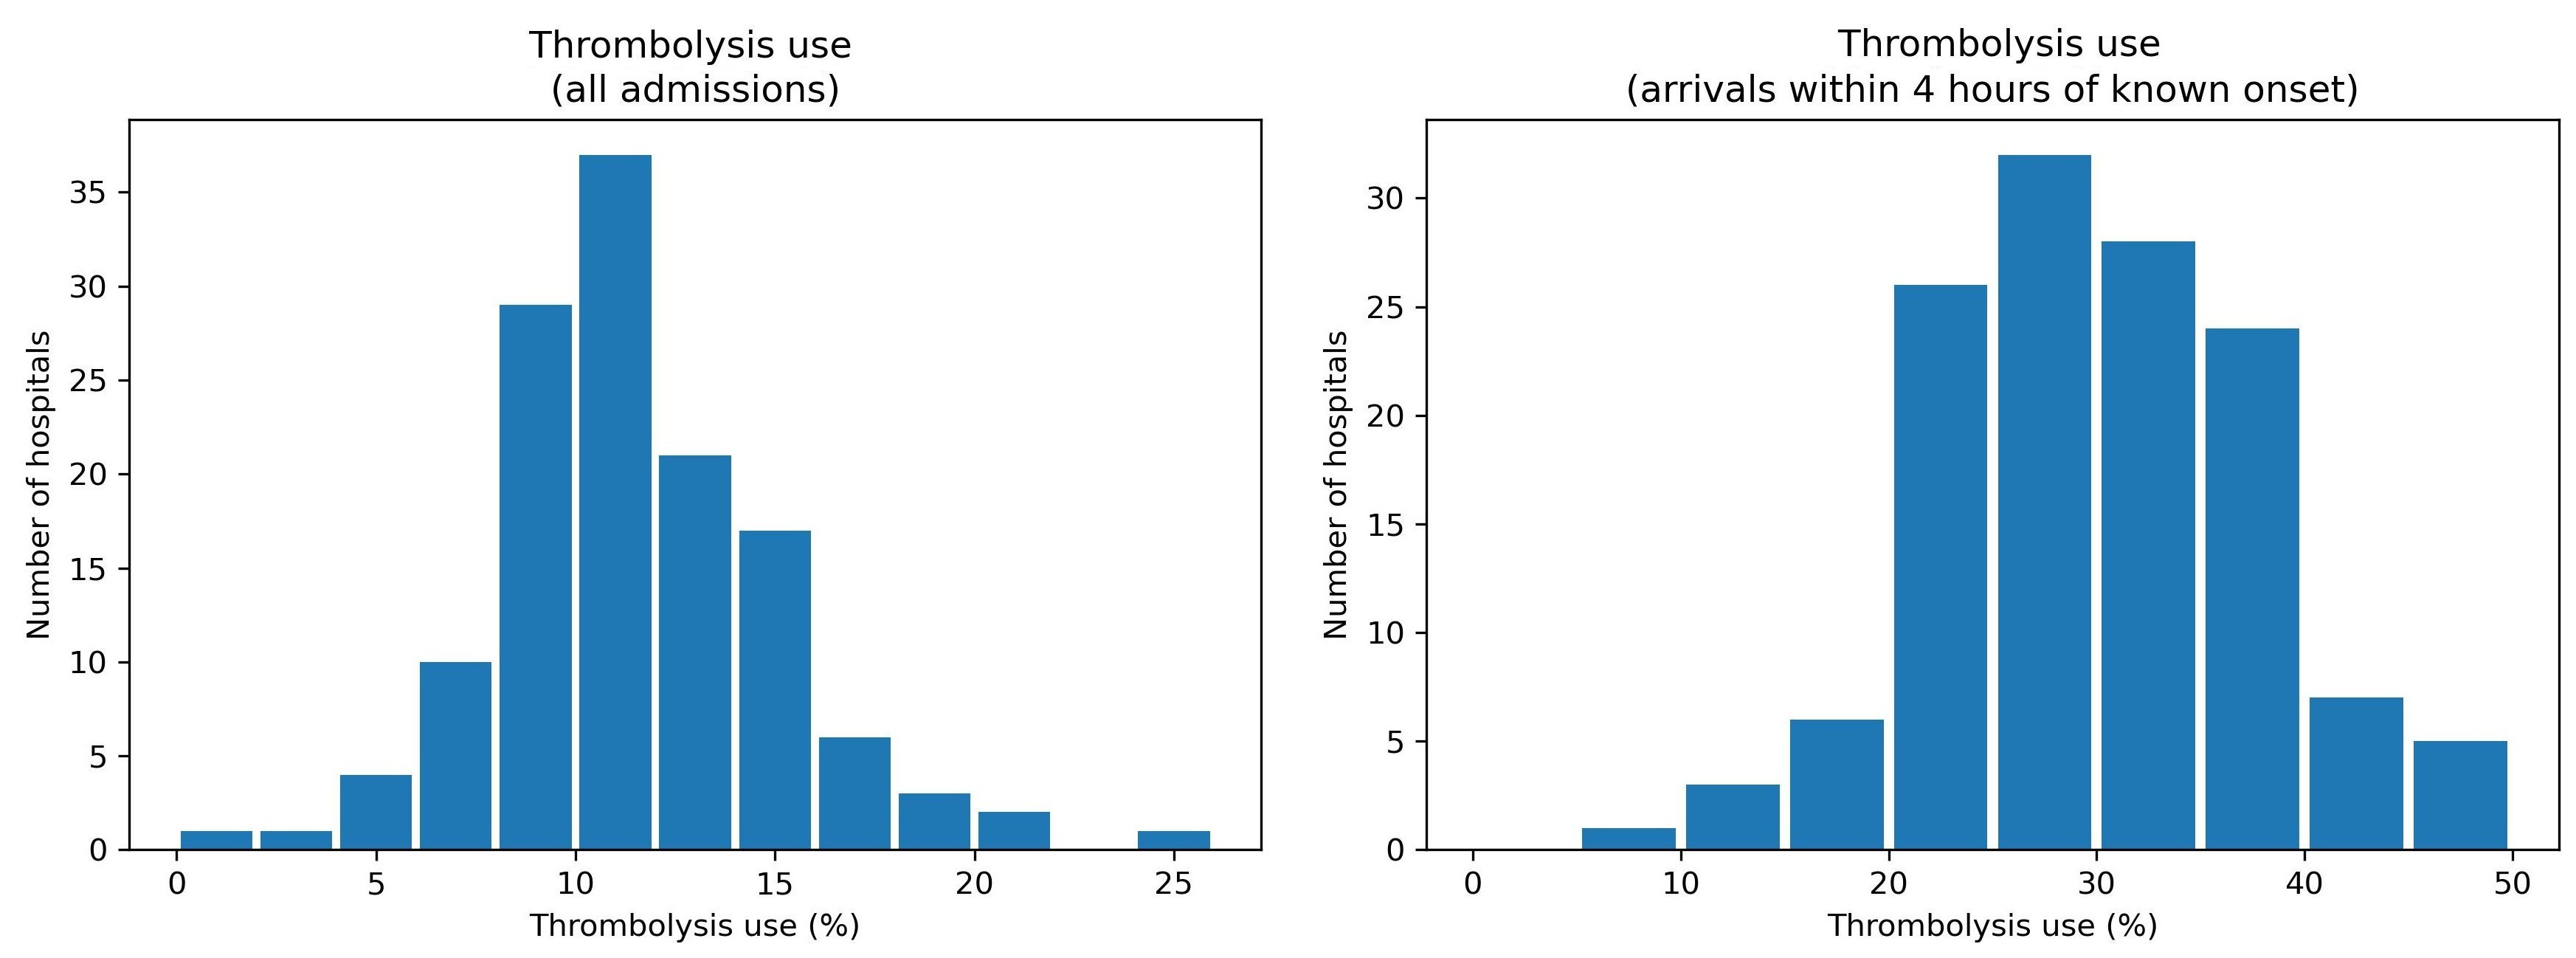
\includegraphics[width=1.0\textwidth]{./images/thrombolysis_hist}
\caption{Histogram of observed thrombolysis use in 132 hospitals. Left: Thrombolysis shown as a percentage of all emergency stroke admissions. Right: Thrombolysis shown as a percentage of those patients who arrive at hospitals within 4 hours of known stroke onset.}
\label{fig:observed_thrombolysis_appendix}
\end{figure}

%%%%%%%%%%%%%%%%%%%%%%%%%%%%%%%%%%%%%%%%%%%%%%%%%%%%%%%%%%%%%%%%%%%%%%%%%%%%%%%%%%%%%%%
\subsection{Machine learning methods}

All work was conducted in Python (v3.8). All code is available at: \url{https://github.com/samuel-book/samuel_shap_paper_1}.

Our machine learning model used XGBoost (\emph{eXtreme Gradient Boosting}, v1.5, \url{https://pypi.org/project/xgboost/}). We used default settings apart from *learning rate* was set at 0.5 (see section \ref{sec:fine_tune}).

Machine learning models were explained using SHAP (\emph{SHapley Additive exPlanations}, v0.41 \url{https://pypi.org/project/shap/}). 

%%%%%%%%%%%%%%%%%%%%%%%%%%%%%%%%%%%%%%%%%%%%%%%%%%%%%%%%%%%%%%%%%%%%%%%%%%%%%%%%%%%%%%%

\subsection{Feature selection}

A simplified model was created by using \emph{forward feature selection} where features were added in accordance to how much each one improved the Receiver Operating Characteristic (ROC) Area Under Curve (AUC). ROC AUC was measured using stratified k-fold validation (k=5). A model with all available 84 features had an ROC AUC of 0.922. A model with 10 features had an ROC AUC of 0.919.

The 10 features selected (Figure \ref{fig:feature_selection}) were:

\begin{itemize}
    \item \emph{Arrival-to-scan time}: Time from arrival at hospital to scan (mins)
    \item \emph{Infarction}: Stroke type (1 = infarction, 0 = haemorrhage)
    \item \emph{Stroke severity}: Stroke severity (NIHSS) on arrival
    \item \emph{Precise onset time}: Onset time type (1 = precise, 0 = best estimate)
    \item \emph{Prior disability level}: Disability level (modified Rankin Scale) before stroke
    \item \emph{Stroke team}: Stroke team attended
    \item \emph{Use of AF anticoagulants}: Use of atrial fibrillation anticoagulant (1 = Yes, 0 = No)
    \item \emph{Onset-to-arrival time}: Time from onset of stroke to arrival at hospital (mins)
    \item \emph{Onset during sleep}: Did stroke occur in sleep?
    \item \emph{Age}: Age (as middle of 5 year age bands)
\end{itemize}

\begin{figure}
\centering
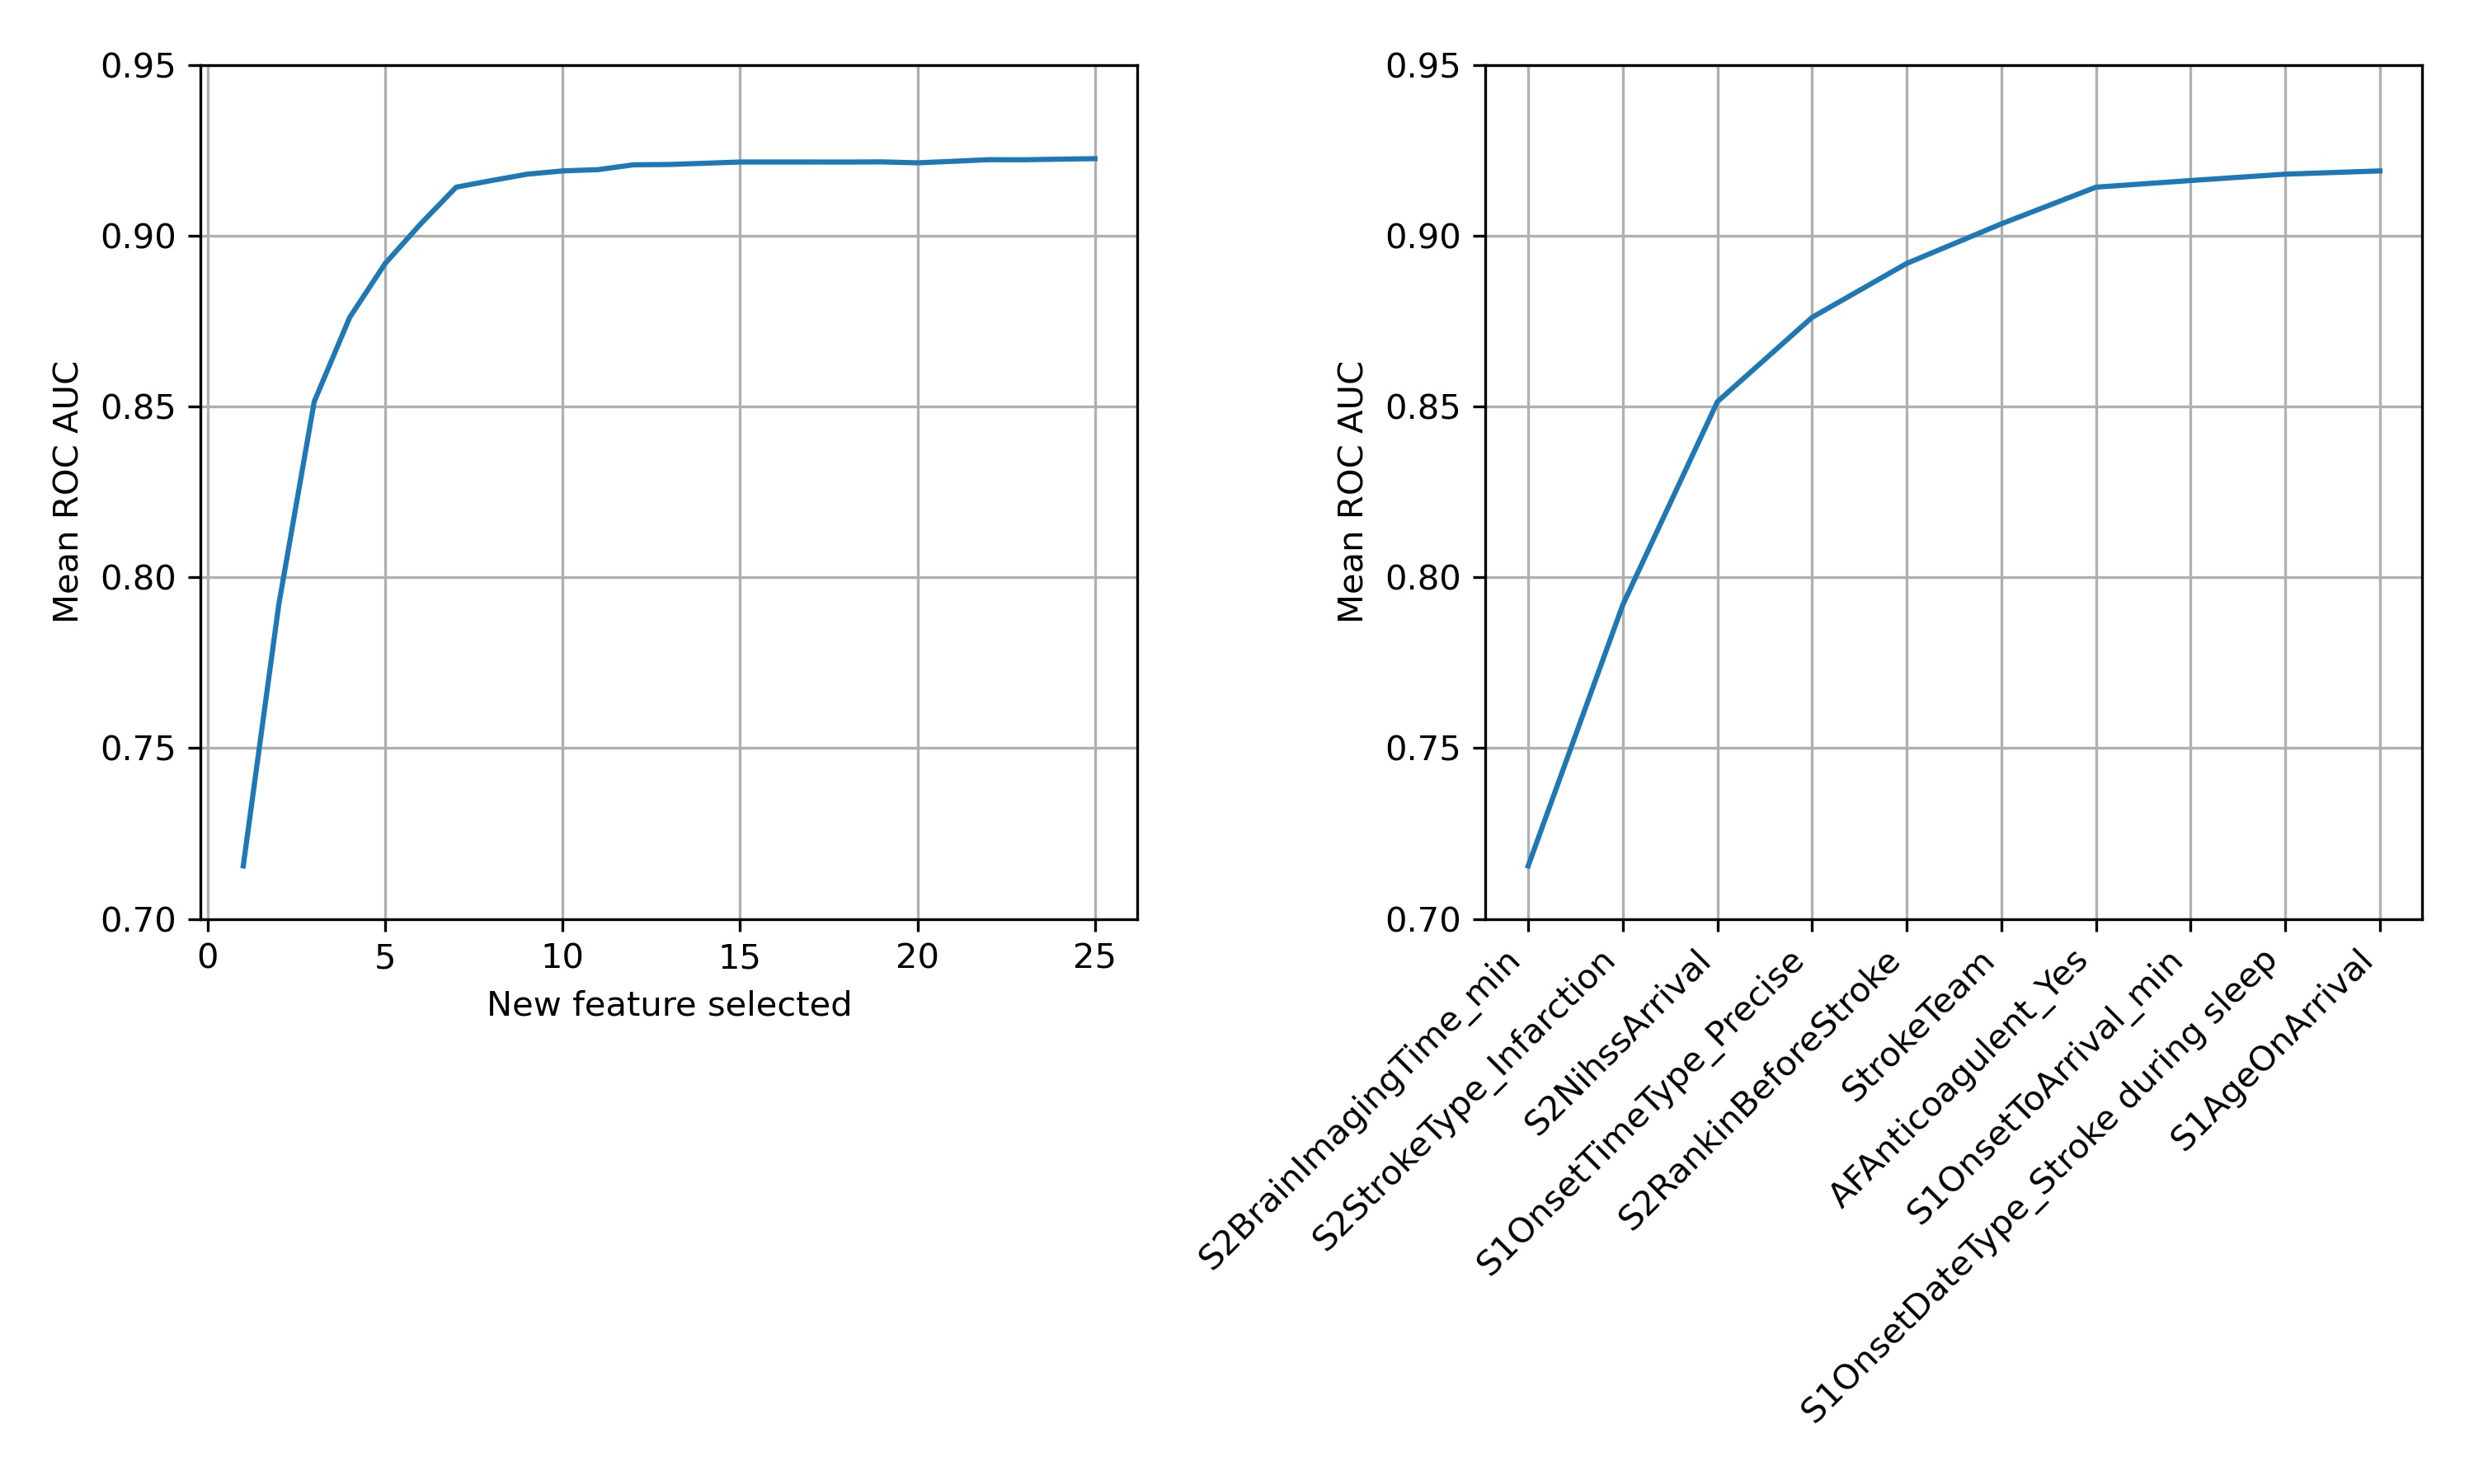
\includegraphics[width=1\textwidth]{./images/01_feature_selection}
\caption{The effect of increasing the number of features on model accuracy measured by Receiver Operating Characteristic (ROC) Area Under Curve (AUC). Left: Improvement with ROC AUC with selection of up to 25 features. Right: Improvement with ROC AUC with selection of the best 10 features. ROC was measured with stratified 5-fold cross-validation. Results show the mean of the 5-fold replicates.}
\label{fig:feature_selection}
\end{figure}


\vspace{5mm}

\begin{center}
    \textbf{\large{NOTE: All results from this point forward will use the 10 feature model.}}
\end{center}




%%%%%%%%%%%%%%%%%%%%%%%%%%%%%%%%%%%%%%%%%%%%%%%%%%%%%%%%%%%%%%%%%%%%%%%%%%%%%%%%%%%%%%%

\subsection{Correlations within the 10 selected features}

Correlations between the 10 features were measured using coefficients of determination (r-squared). All r-squared were less than 0.15, and all r-squared were less than 0.05 except 1) age and prior disability level (r-squared 0.146), and 2) onset during sleep and precise onset time (r-squared 0.078). All correlations are shown in table \ref{tab:correl}.


\begin{longtable}[]{@{}rrr@{}}
\caption{Correlations between the 10 features selected for the XGBoost machine learning model.}\\
\toprule
Variable 1 & Variable 2 & r-squared\tabularnewline
\midrule
\endhead
Age & Prior disability level & 0.1462\tabularnewline
Onset during sleep & Precise onset time & 0.0784\tabularnewline
Stroke severity & Prior disability level & 0.0454\tabularnewline
Stroke severity & Infarction & 0.0386\tabularnewline
Precise onset time & Onset-to-arrival time & 0.0344\tabularnewline
Stroke severity & Age & 0.0268\tabularnewline
Age & Use of AF anticoagulants & 0.0207\tabularnewline
Stroke severity & Onset-to-arrival time & 0.0186\tabularnewline
Precise onset time & Prior disability level & 0.0131\tabularnewline
Age & Precise onset time & 0.0090\tabularnewline
Prior disability level & Use of AF anticoagulants &
0.0070\tabularnewline
Onset during sleep & Onset-to-arrival time & 0.0043\tabularnewline
Onset-to-arrival time & Age & 0.0038\tabularnewline
Use of AF anticoagulants & Infarction & 0.0033\tabularnewline
Prior disability level & Onset-to-arrival time & 0.0022\tabularnewline
Precise onset time & Arrival-to-scan time & 0.0021\tabularnewline
Use of AF anticoagulants & Stroke severity & 0.0019\tabularnewline
Arrival-to-scan time & Stroke severity & 0.0019\tabularnewline
Precise onset time & Use of AF anticoagulants & 0.0016\tabularnewline
Stroke severity & Onset during sleep & 0.0011\tabularnewline
Infarction & Onset-to-arrival time & 0.0007\tabularnewline
Infarction & Onset during sleep & 0.0007\tabularnewline
Infarction & Precise onset time & 0.0006\tabularnewline
Onset-to-arrival time & Arrival-to-scan time & 0.0004\tabularnewline
Arrival-to-scan time & Prior disability level & 0.0001\tabularnewline
Onset-to-arrival time & Use of AF anticoagulants & 0.0001\tabularnewline
Stroke severity & Precise onset time & 0.0000\tabularnewline
Arrival-to-scan time & Age & 0.0000\tabularnewline
Use of AF anticoagulants & Onset during sleep & 0.0000\tabularnewline
Prior disability level & Onset during sleep & 0.0000\tabularnewline
Infarction & Age & 0.0000\tabularnewline
Use of AF anticoagulants & Arrival-to-scan time & 0.0000\tabularnewline
Onset during sleep & Arrival-to-scan time & 0.0000\tabularnewline
Arrival-to-scan time & Infarction & 0.0000\tabularnewline
Age & Onset during sleep & 0.0000\tabularnewline
Prior disability level & Infarction & 0.0000\tabularnewline
\bottomrule
\label{tab:correl}
\end{longtable}


%%%%%%%%%%%%%%%%%%%%%%%%%%%%%%%%%%%%%%%%%%%%%%%%%%%%%%%%%%%%%%%%%%%%%%%%%%%%%%%%%%%%%%%

\subsection{Model accuracy}

Model accuracy was measured using stratified 5-fold cross validation. The key results are shown in table \ref{tab:accuracy_appendix}.

\begin{minipage}{\textwidth}
\begin{longtable}[]{@{}lll@{}}
\caption{Accuracy of 10 feature XGBoost model in predicting thrombolysis use in patients arriving at hospital within 4 hours of known stroke onset.}\\
\toprule
Accuracy measurement & mean & std\tabularnewline
\midrule
\endhead
Actual positive rate & 0.296 & 0.000\tabularnewline
Actual negative rate & 0.704 & 0.000\tabularnewline
Predicted positive rate & 0.294 & 0.002\tabularnewline
Predicted negative rate & 0.706 & 0.002\tabularnewline
Accuracy & 0.850 & 0.004\tabularnewline
Sensitivity (recall) & 0.743 & 0.004\tabularnewline
Specificity & 0.894 & 0.004\tabularnewline
Precision & 0.747 & 0.007\tabularnewline
ROC AUC & 0.918 & 0.003\tabularnewline
Balanced sensitivity/specificity & 0.839 & 0.003\tabularnewline
\bottomrule
\label{tab:accuracy_appendix}
\end{longtable}
\end{minipage}

We found an overall accuracy of 85/%, with a balanced accuracy. The predicted thrombolysis rate of 29.4/% was very close to the observed thrombolysis rate of 29.6/%.

Figure \ref{fig:roc} shows the receiver operating characteristic curve, along with the trade-off between sensitivity and specificity.

\begin{figure}
\centering
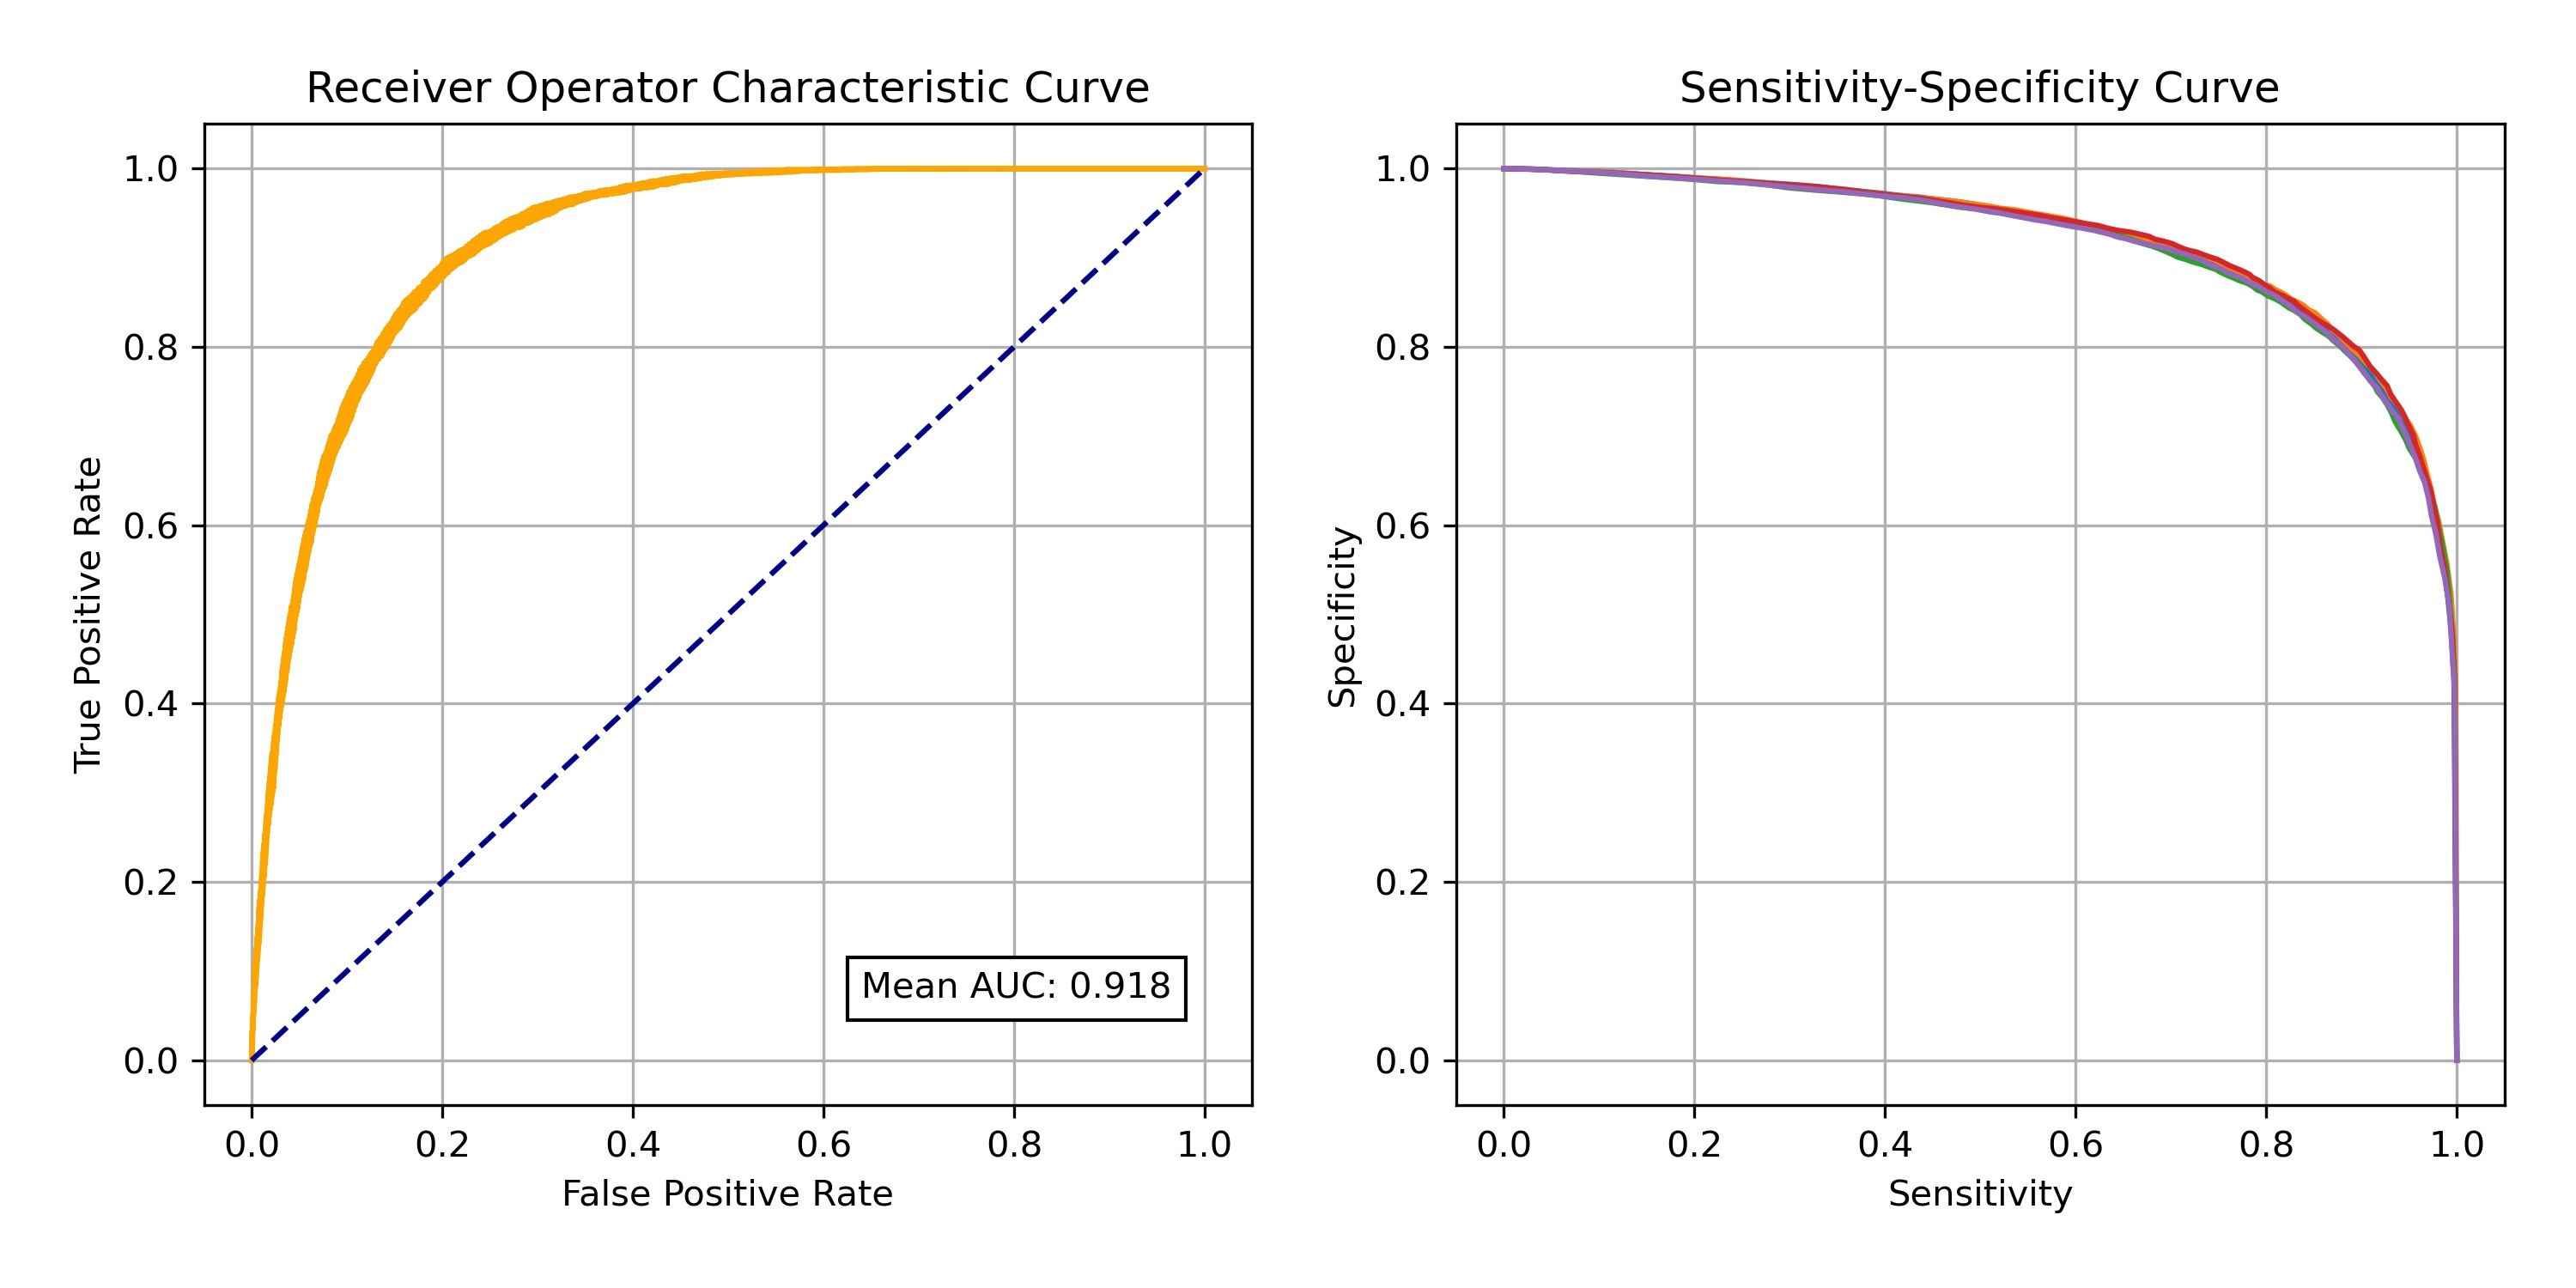
\includegraphics[width=1\textwidth]{./images/02_xgb_10_features_roc_sens_spec}
\caption{Model accuracy of a XGBoost model using 10 features. Left: Receiver Operating Characteristic (ROC) Area Under Curve (AUC). Right: The trade-off between Sensitivity and Specificity. Accuracy was measured with stratified 5-fold cross-validation, and both charts show all 5 k-fold replicates.}
\label{fig:roc}
\end{figure}


%%%%%%%%%%%%%%%%%%%%%%%%%%%%%%%%%%%%%%%%%%%%%%%%%%%%%%%%%%%%%%%%%%%%%%%%%%%%%%%%%%%%%%%

\subsection{Validation of hospital thrombolysis use}

With k-fold validation, every instance is in one, but only one, test set. The test sets may therefore be combined to have predictions for the whole data set. Using these collated results we compared predicted thrombolysis use at each hospital with the actual (observed) thrombolysis use (figure \ref{fig:thrombolysis_pred_observed}. There was very good agreement between predicted and observed thrombolysis use at each hospital (r-squared 0.977).

\begin{figure}
\centering
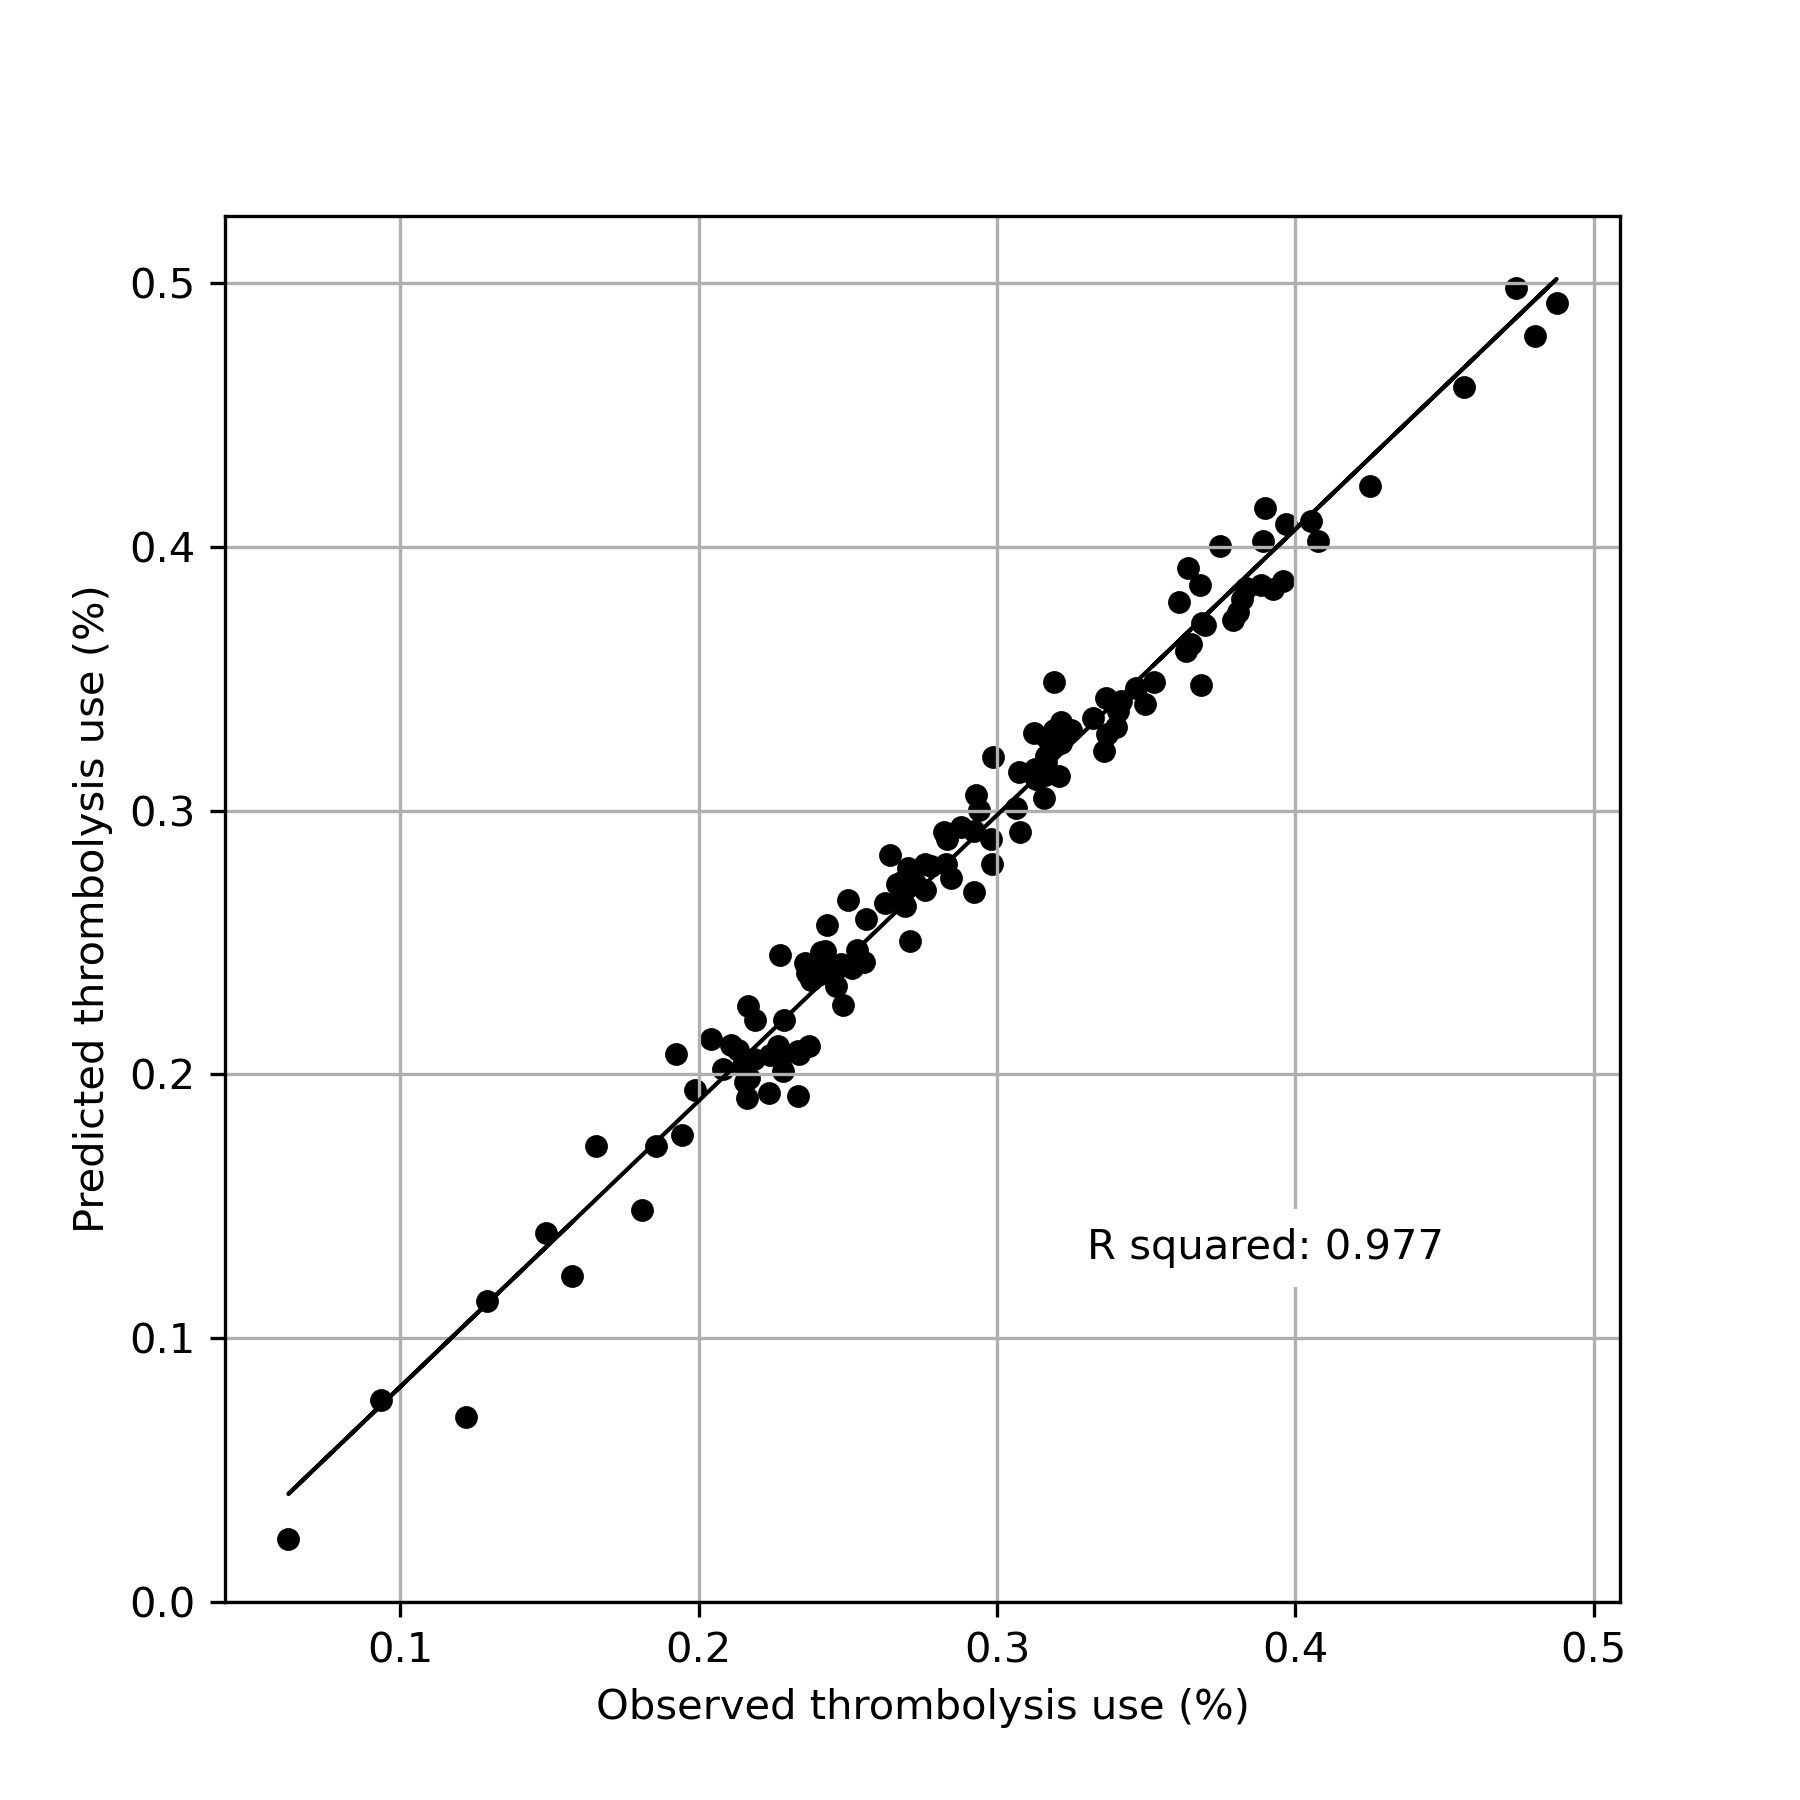
\includegraphics[width=0.6\textwidth]{./images/02_xgb_10_features_observed_predicted_rates}
\caption{Comparison of predicted and observed thrombolysis use for 132 hospitals.}
\label{fig:thrombolysis_pred_observed}
\end{figure}


%%%%%%%%%%%%%%%%%%%%%%%%%%%%%%%%%%%%%%%%%%%%%%%%%%%%%%%%%%%%%%%%%%%%%%%%%%%%%%%%%%%%%%%

\subsection{Model calibration}

The model calibration was checked by binning predictions by probability, and comparing the mean predicted probability with the fraction that were actually positive (table \ref{tab:calibration} and figure \ref{fig:calibration}). In a well-calibrated model, in each bin the average probability of receiving thrombolysis should be close to the proportion of patients who actually received thrombolysis. Results demonstrated that the model was naturally well-calibrated, and was not in need of any calibration correction. As expected, the fraction of predictions that were correct is related to the predicted probability of receiving thrombolysis (when predictions were close to 50\% probability of receiving thrombolysis the model was correct about 50\% of the time, whereas when the model had predictions of <10\% or >90\% probability of receiving thrombolysis, the model was be correct about 90\% of the time).

Nearly 50\% of patients fell in the 0-10\% probability of receiving thrombolysis - that is the model gave a confident prediction that the these patients would not receive thrombolysis, with the model being correct in these predictions 98\% of the time.

\begin{minipage}{\textwidth}
\begin{longtable}[]{@{}lllll@{}}
\caption{Model calibration based on binning by predicted probability of thrombolysis.}\\
\toprule
Bin & Predicted probability & Fraction positive & Fraction correct &
Frequency\tabularnewline
\midrule
\endhead
0.0 - 0.1 & 0.018 & 0.023 & 0.977 & 0.480\tabularnewline
0.1 - 0.2 & 0.146 & 0.174 & 0.826 & 0.082\tabularnewline
0.2 - 0.3 & 0.248 & 0.271 & 0.729 & 0.056\tabularnewline
0.3 - 0.4 & 0.348 & 0.371 & 0.629 & 0.045\tabularnewline
0.4 - 0.5 & 0.450 & 0.443 & 0.557 & 0.043\tabularnewline
0.5 - 0.6 & 0.551 & 0.546 & 0.546 & 0.042\tabularnewline
0.6 - 0.7 & 0.652 & 0.643 & 0.643 & 0.049\tabularnewline
0.7 - 0.8 & 0.753 & 0.736 & 0.736 & 0.065\tabularnewline
0.8 - 0.9 & 0.852 & 0.827 & 0.827 & 0.089\tabularnewline
0.9 - 1.0 & 0.932 & 0.893 & 0.893 & 0.049\tabularnewline
\bottomrule
\label{tab:calibration}
\end{longtable}
\end{minipage}


\begin{figure}
\centering
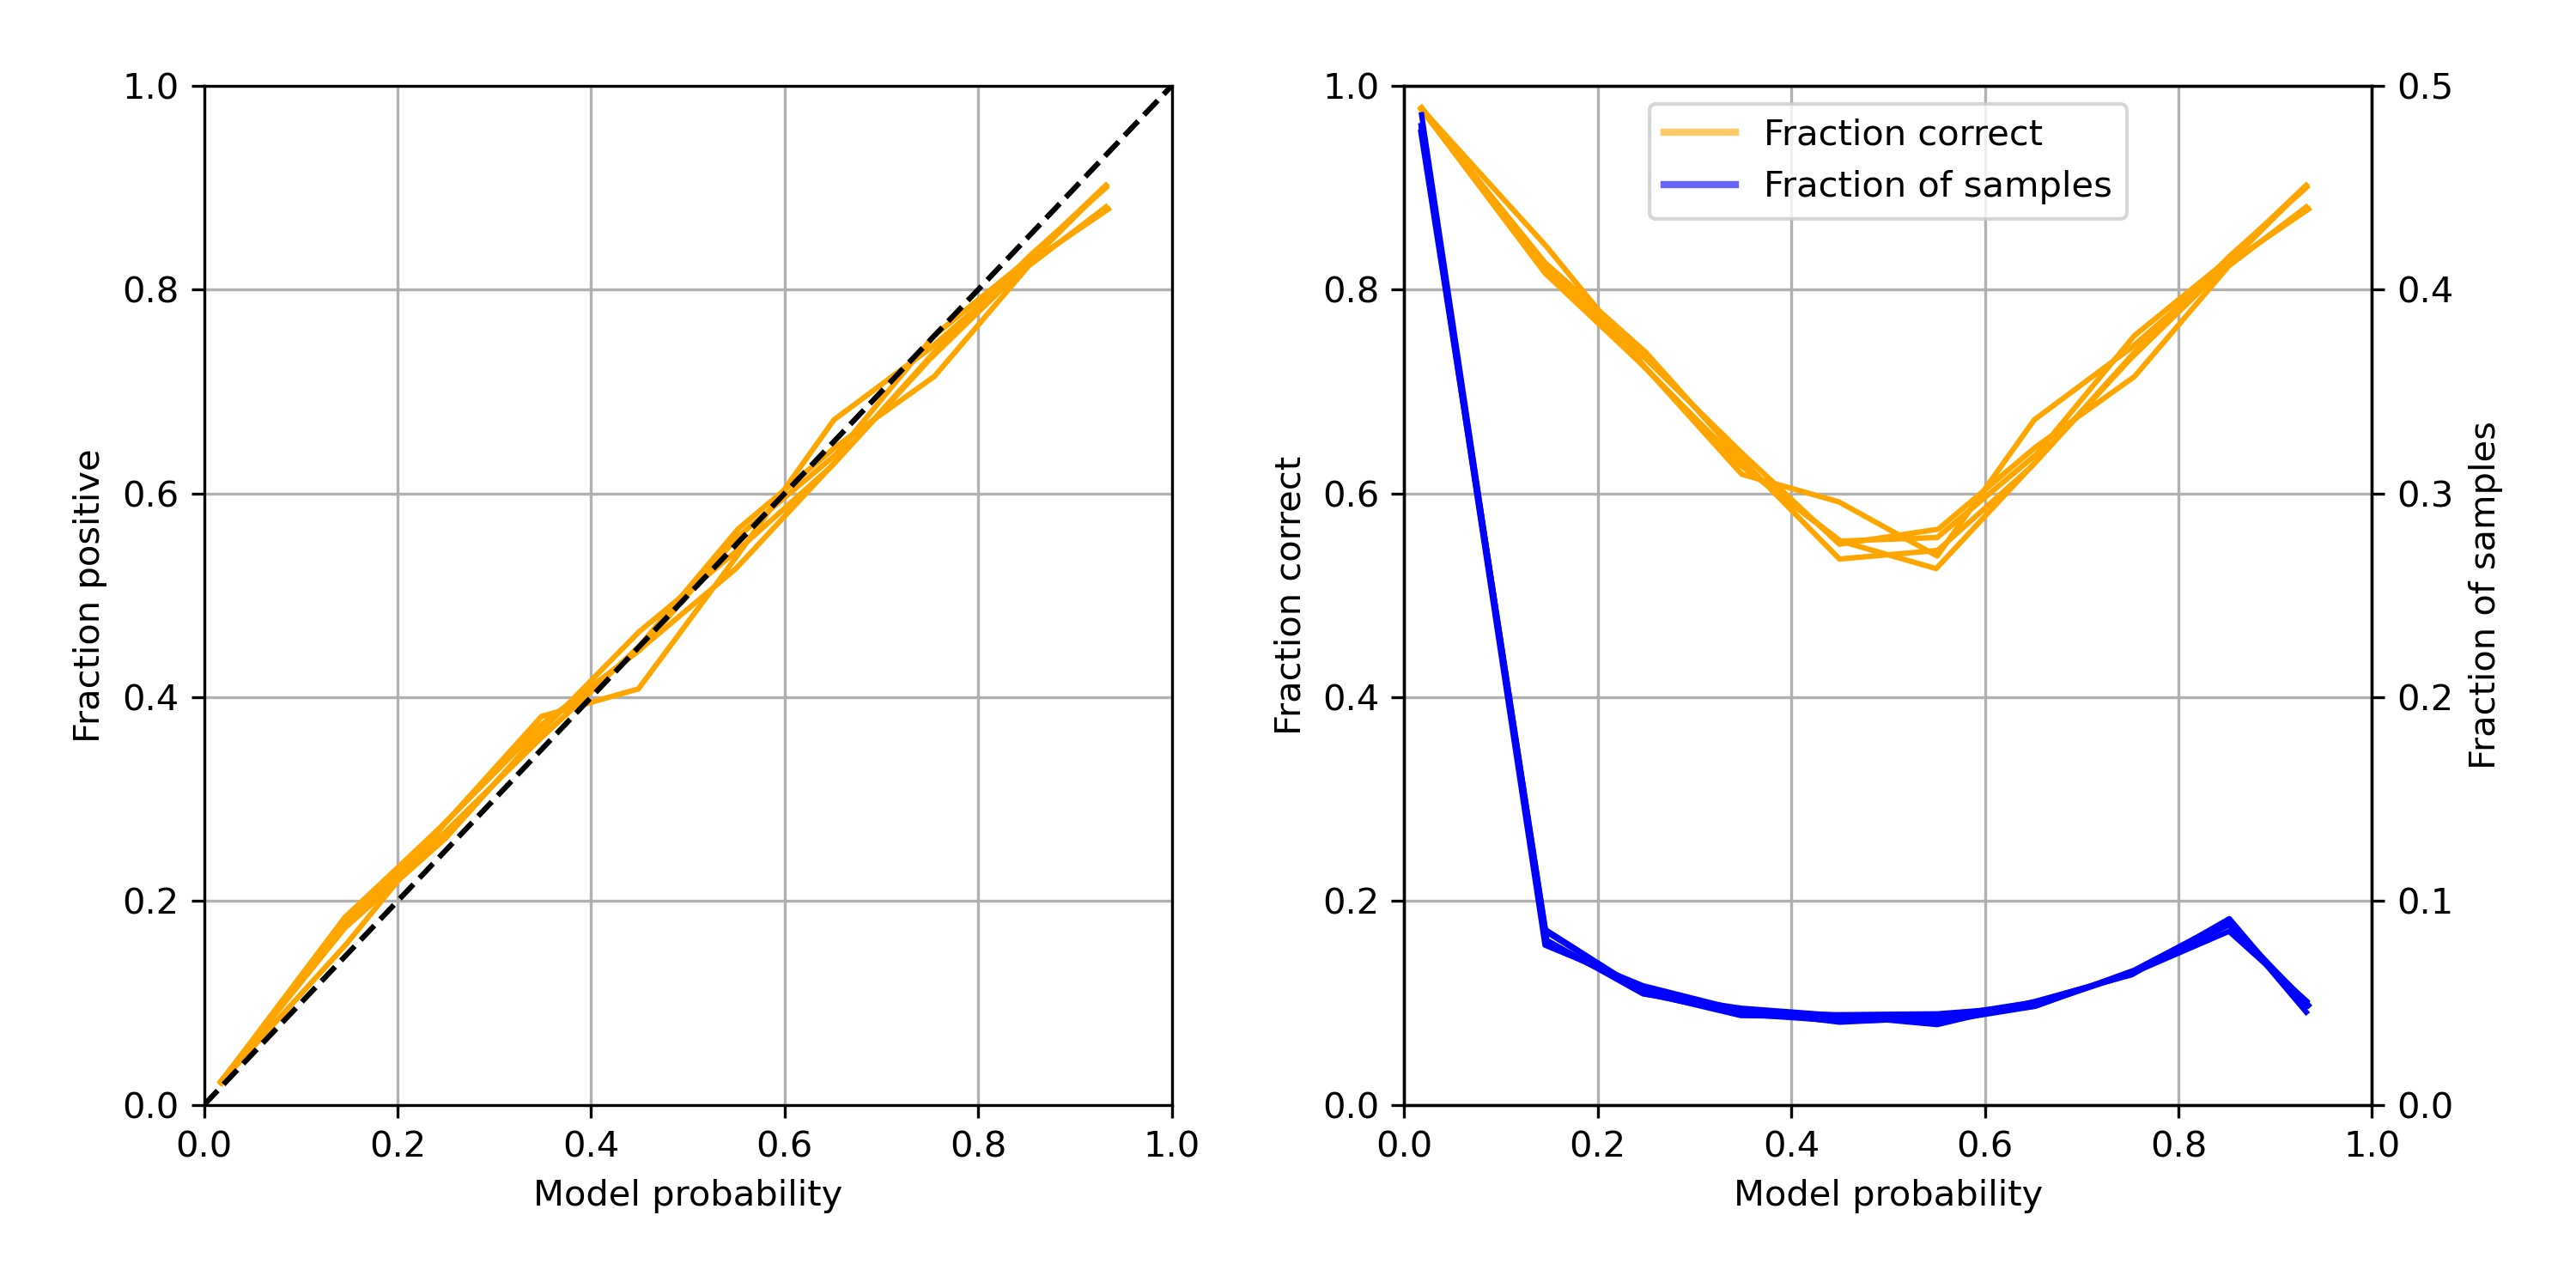
\includegraphics[width=1\textwidth]{./images/02_xgb_10_features_reliability}
\caption{Calibration check of the model. Left: The proportion of patients receiving thrombolysis for binned probability of receiving thrombolysis. Right: The proportion of predictions in each bin (blue), and the proportion of predictions that are correct (orange). Plot show results for all 5 k-fold replicates.}
\label{fig:calibration}
\end{figure}


%%%%%%%%%%%%%%%%%%%%%%%%%%%%%%%%%%%%%%%%%%%%%%%%%%%%%%%%%%%%%%%%%%%%%%%%%%%%%%%%%%%%%%%

\subsection{Evaluating variation in model predictions and predicted 10k cohort thrombolysis rate using bootstrap models}

Data was split into a training set of 78,928 patients, and a test set of 10k patients. 30 models were trained, each with a different bootstrap sample of the training set and with a different model random seed. For each of the 10k test set, we evaluated the variation in the predicted probability of receiving thrombolysis (figure \ref{fig:bootstrap_1}. The mean of these standard deviations was 0.057, but the variation depended on the probability, with variation peaking at about 0.13 when the prediction probability of receiving thrombolysis was around 0.5.

\begin{figure}
\centering
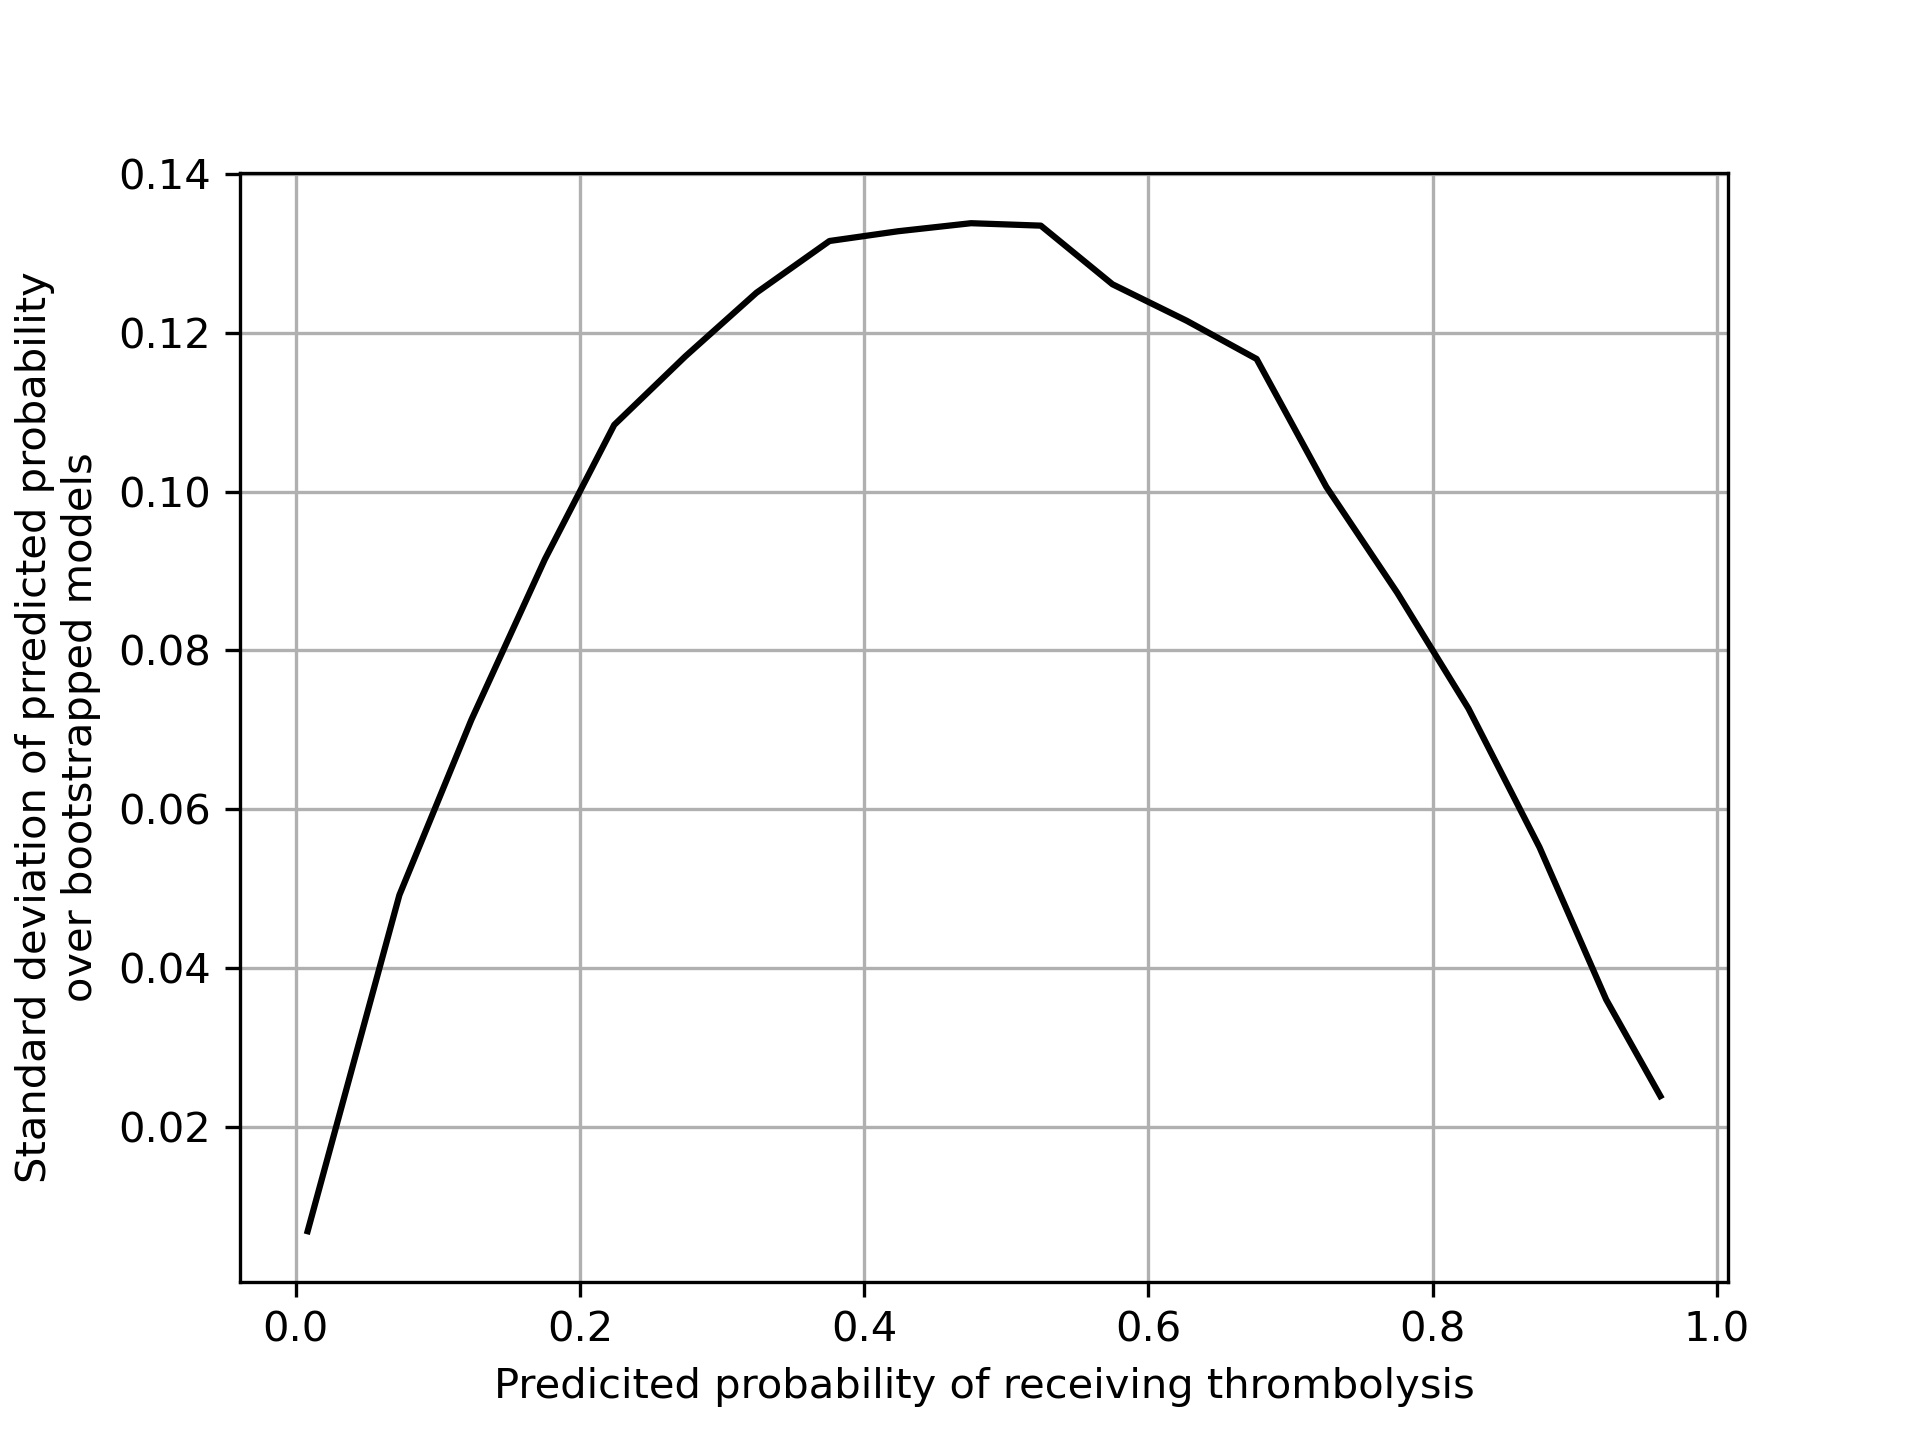
\includegraphics[width=0.7\textwidth]{./images/50_bootstrap_prediction_sd}
\caption{Standard deviation of predicted probability of receiving thrombolysis, from 30 bootstrapped models predicting the probability of receiving thrombolysis in 10k patients. Results are binned by predicted probability.}
\label{fig:bootstrap_1}
\end{figure}

Additionally, we used the models and test set to predict thrombolysis use at each of the 132 hospitals if the 10k cohort of patients had attended each of the hospitals (by changing the hospital one-hot encoding, figure \ref{fig:bootstrap_2}). We predicted the thrombolysis use at each hospital, and examined the variation between the 30 bootstrapped models. The mean of the standard deviation of bootstrap replicates was 1.7\% (where hospital thrombolysis use rates were 10\% to 45\%).

\begin{figure}
\centering
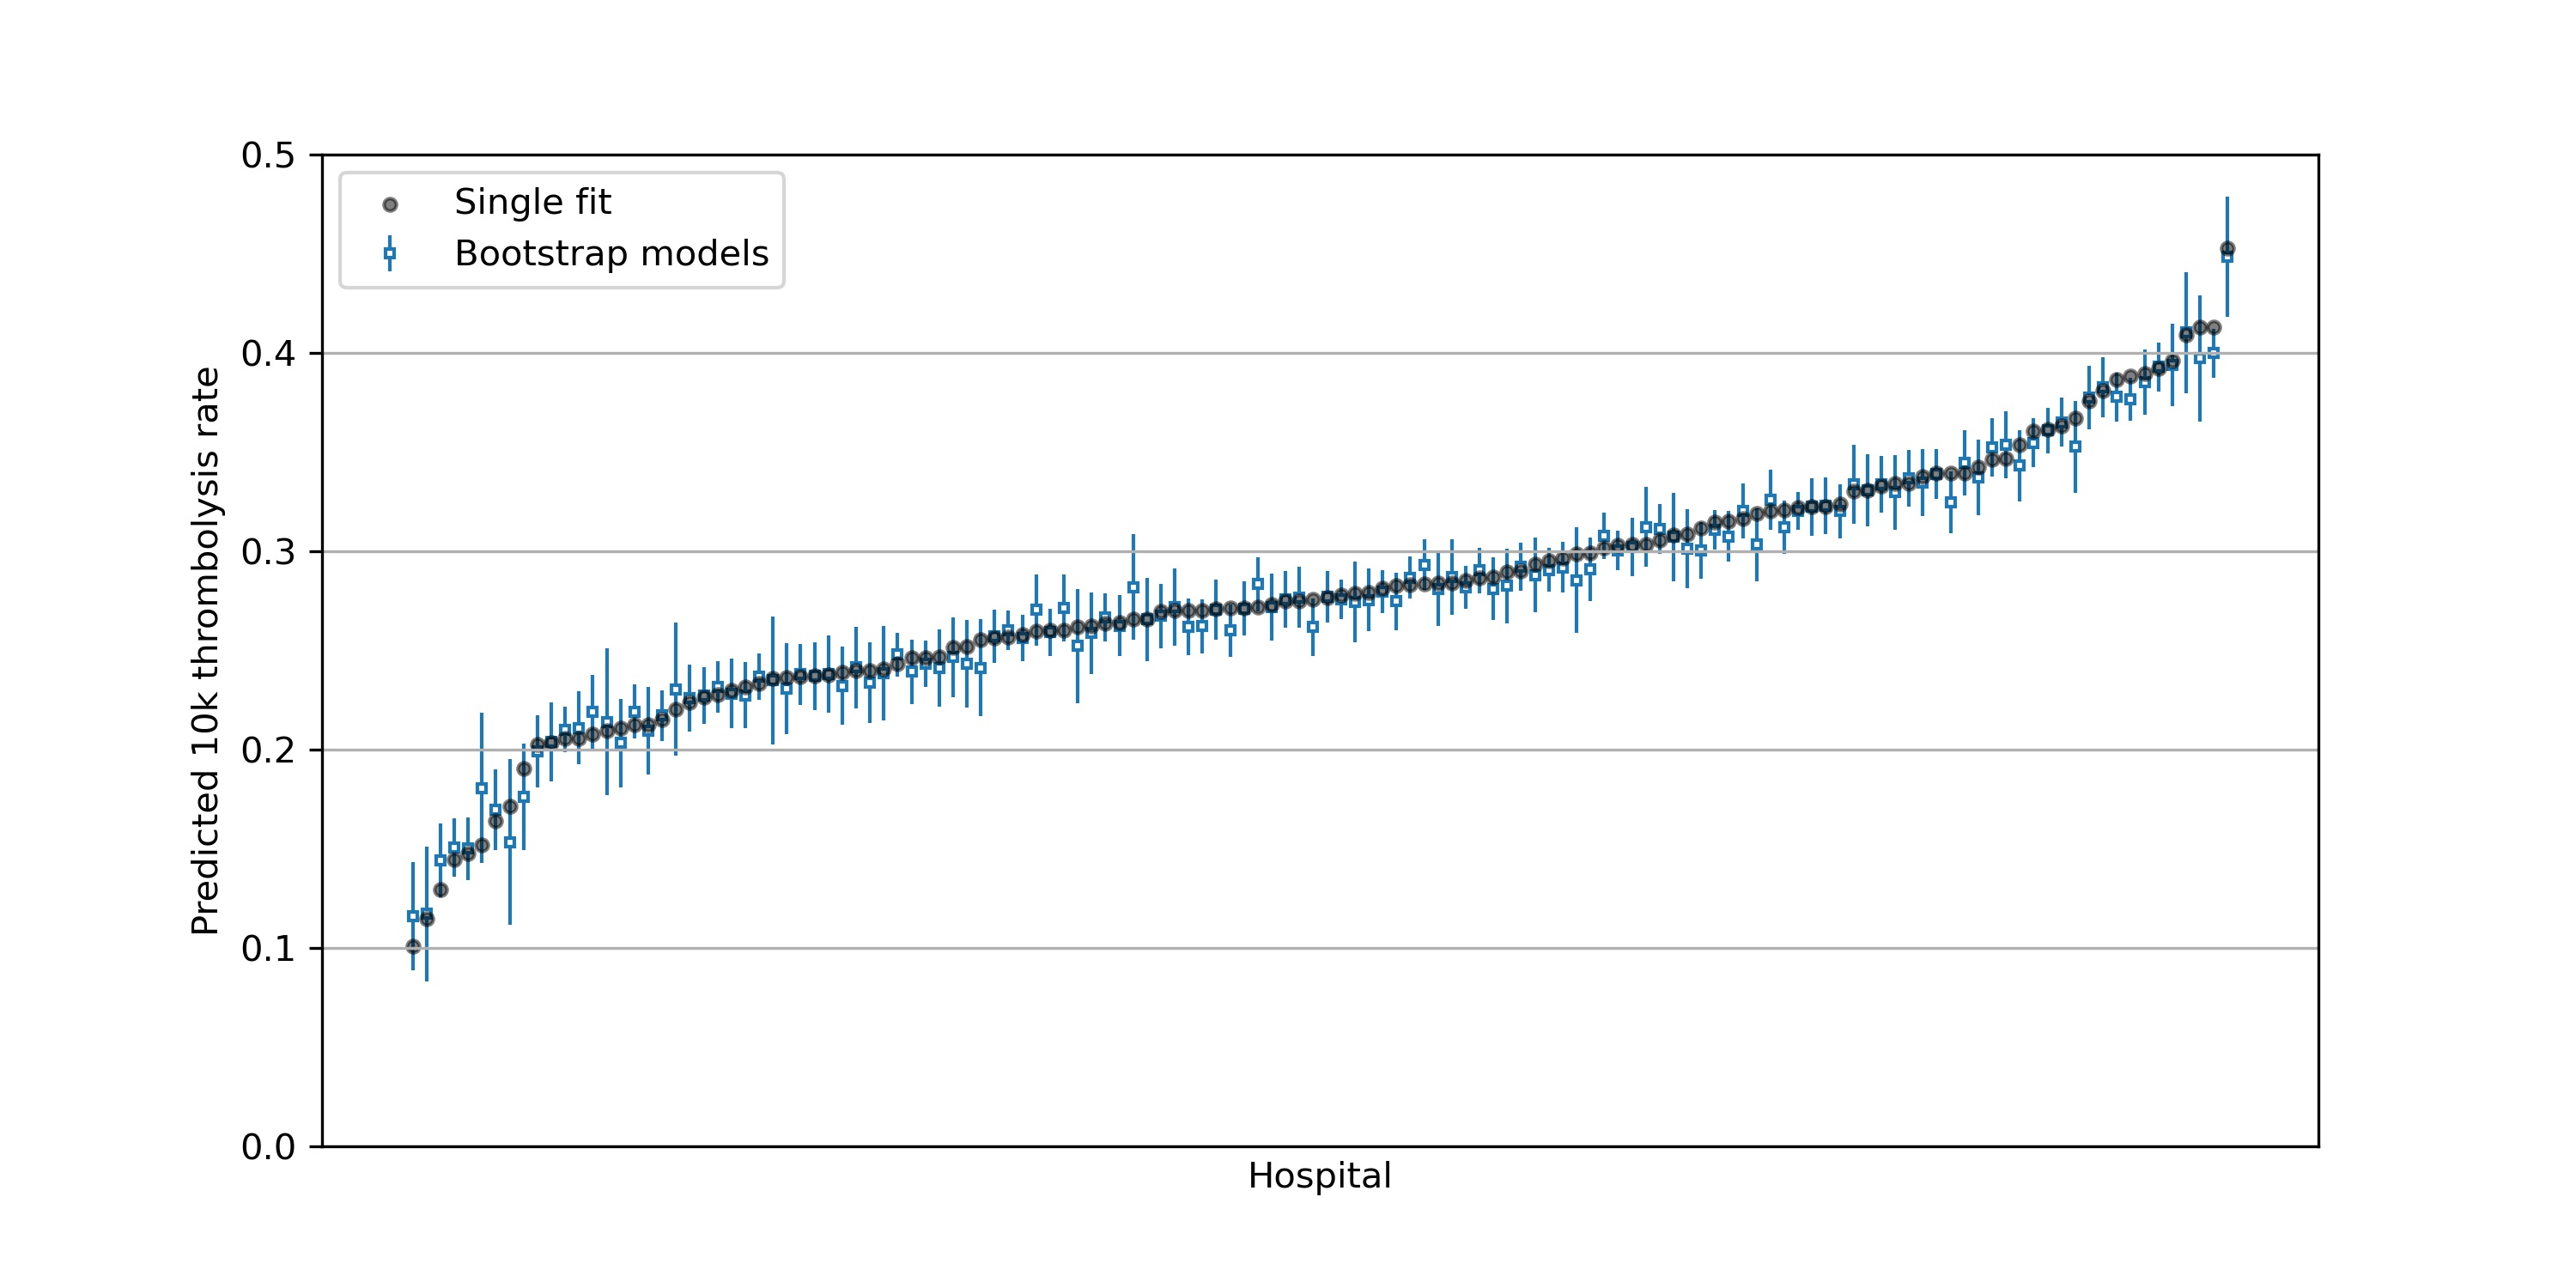
\includegraphics[width=1\textwidth]{./images/50_bootstrap_10k_sd}
\caption{Mean and standard deviation of predicted thrombolysis use at 132 hospitals from 30 bootstrapped models. Results are for predicted thrombolysis use for the same 10k patient cohort for each hospital. In addition to the results for the bagging models, the predicted thrombolysis use for a single model with bootstrap sampling is shown. Results are ordered by thrombolysis use at each hospital predicted from the single non-bootstrap model.}
\label{fig:bootstrap_2}
\end{figure}

Bagging experiments were repeated with \emph{Baysian Bootstrapping} based on weighting training samples using a Dirichlet distribution. Very similar results were achieved, with a mean standard deviation of bootstrap replicate probability predictions of 0.054, and a mean standard deviation of bootstrap replicate 10k thrombolysis use in hospitals of 1.6\%.

The evaluation of bootstrapped replicates gave us confidence that a single model fit would be sufficient. 


%%%%%%%%%%%%%%%%%%%%%%%%%%%%%%%%%%%%%%%%%%%%%%%%%%%%%%%%%%%%%%%%%%%%%%%%%%%%%%%%%%%%%%%

\subsection{Learning curves}

Learning curves evaluate the relationship between training set size and model accuracy. Learning curves were performed using stratified 5-fold validation, and by random sampling (without replacement) of the training set (figure \ref{fig:learning_curve}. The maximum accuracy achieved was 85\% using 70k training instances, 82.5\% accuracy was achieved with 4k training instances. There was a shallow improvement between 4k and 70k training points.

\begin{figure}
\centering
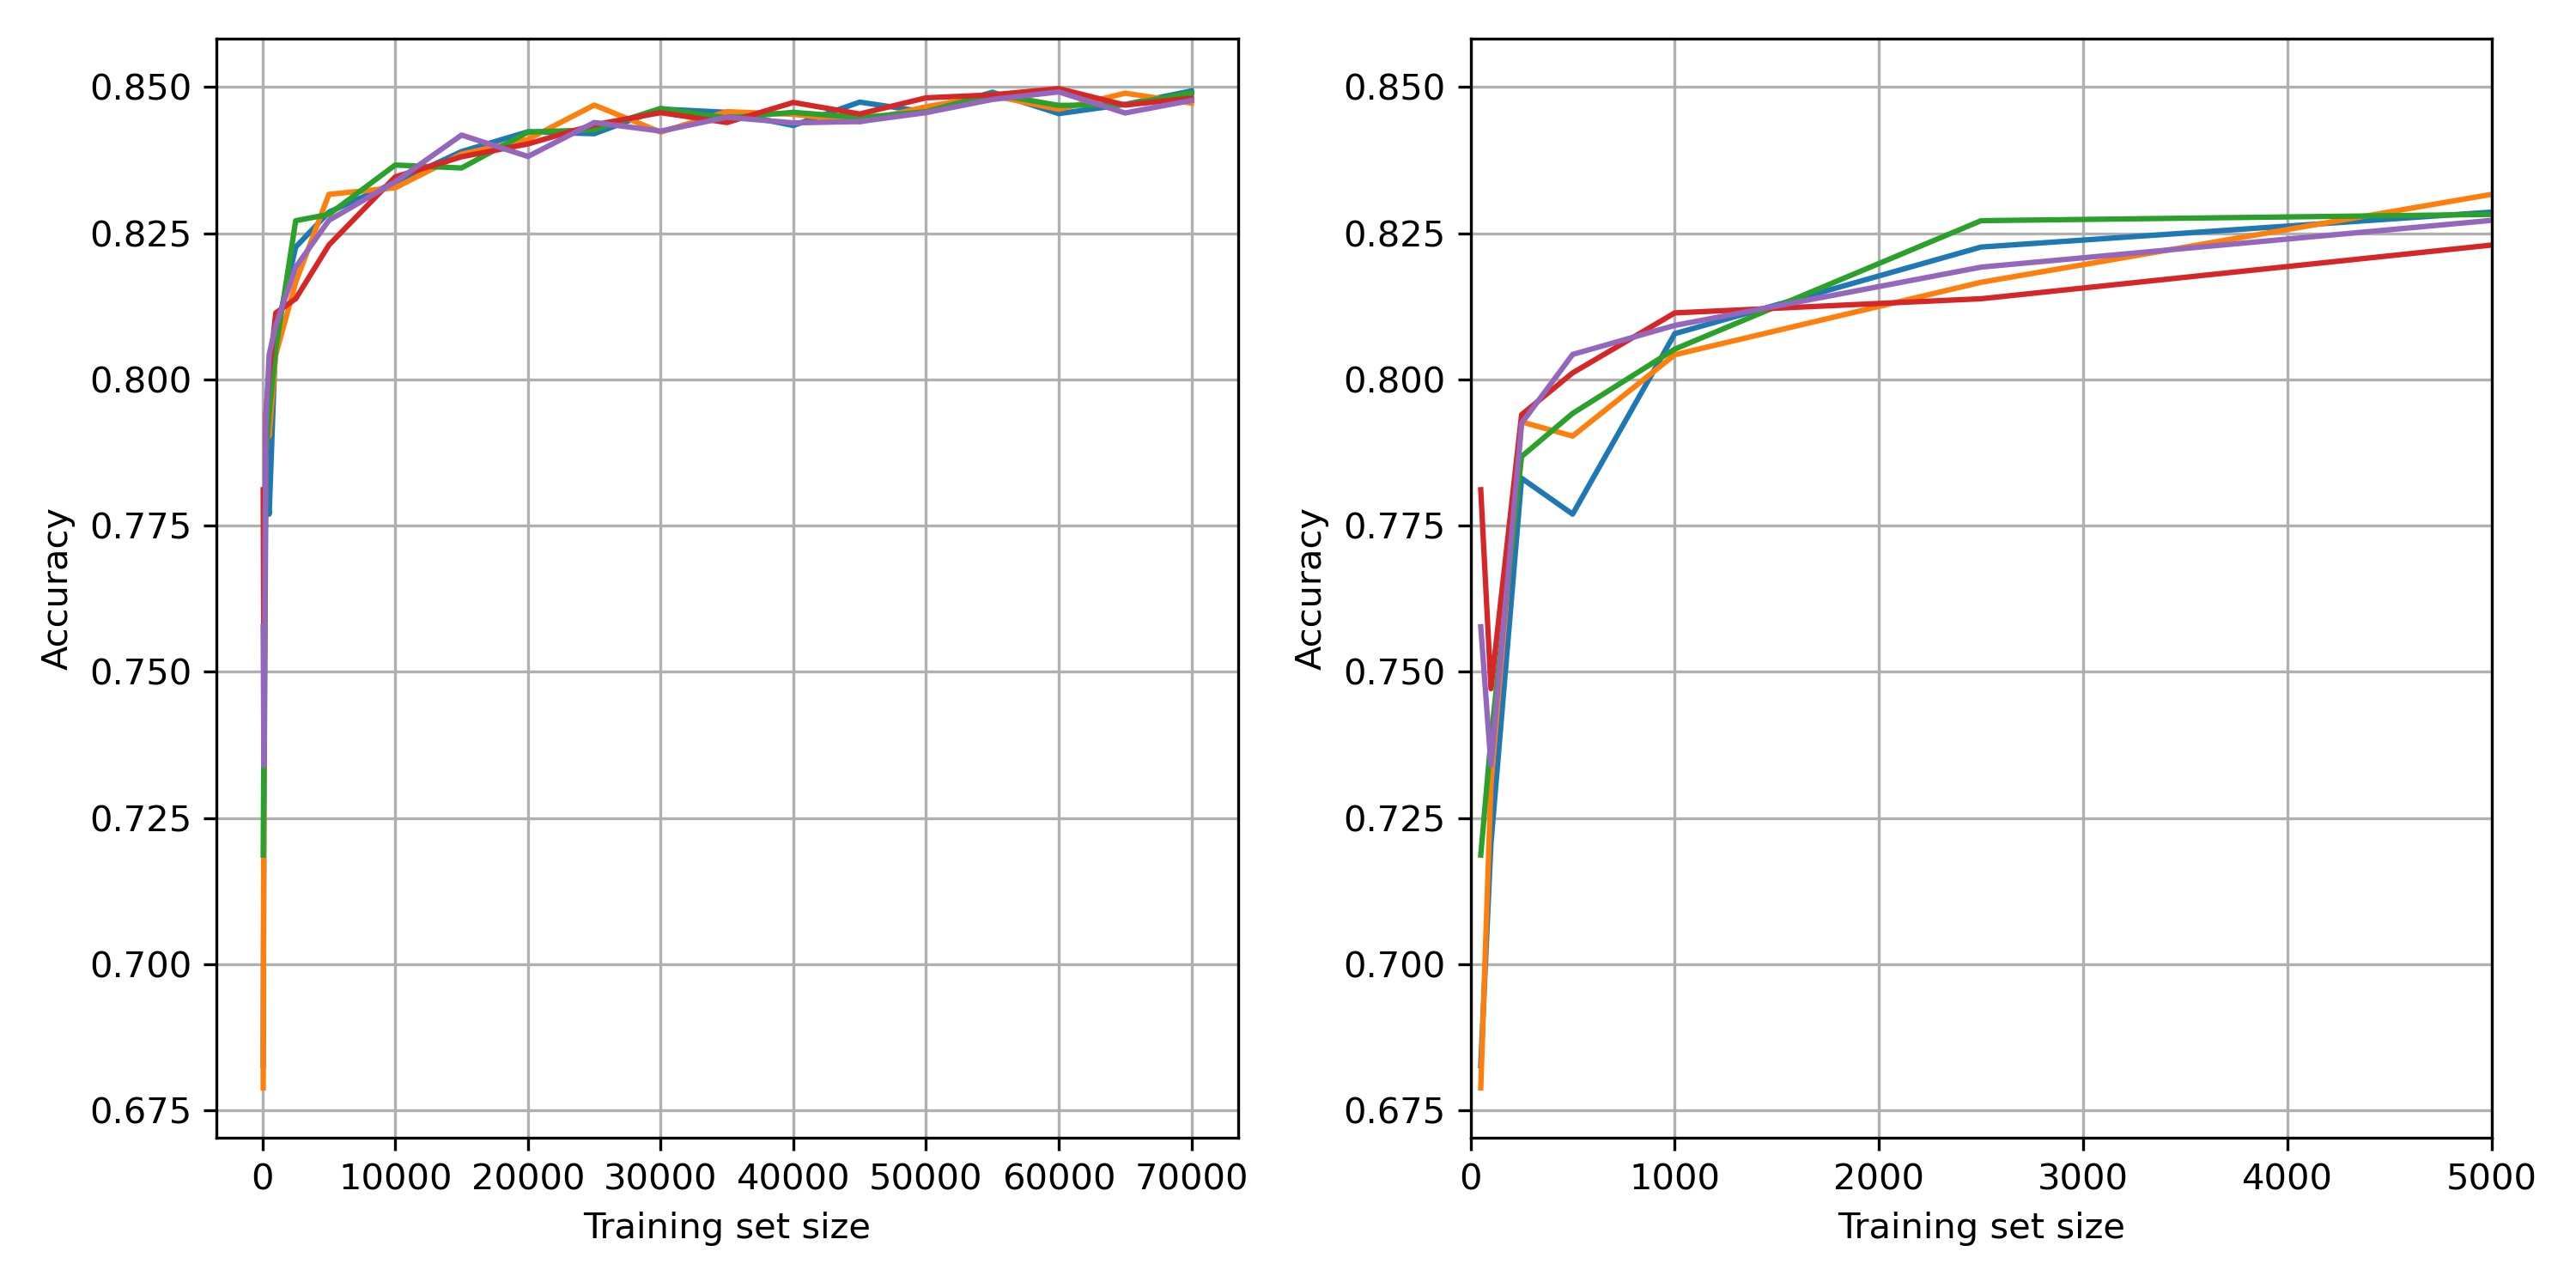
\includegraphics[width=1\textwidth]{./images/02_xgb_10_features_learning_curve}
\caption{Learning curves showing the relationship between training set size and model accuracy. Left: training set size up to 70k. Right: training set size up to 5k (same results as the results on the left). Results are shown for all 5 k-fold replicates.}
\label{fig:learning_curve}
\end{figure}

%%%%%%%%%%%%%%%%%%%%%%%%%%%%%%%%%%%%%%%%%%%%%%%%%%%%%%%%%%%%%%%%%%%%%%%%%%%%%%%%%%%%%%%

\subsection{Fine-tuning of model regularisation}
\label{sec:fine_tune}

As hospital ID is encoded as one-hot, and there are 132 hospitals, it is possible that the effect of hospitals ID becomes 'regularised out', especially as for each one-hot encoded column about 99% of the feature values will be zero. *Learning rate* in XGBoost acts as a regularising method. The lower the learning rate the less weight new trees have, and so the model becomes more regularised (less likely to overfit).

As we are concerned with differences between hospitals, we did not want to over-regularise the model. To optimise *learning rate* we looked at the between-hospital variation of predicted thrombolysis use in a 10k cohort of patients (with the model predicting the use of thrombolysis in each hospital with the same 10k cohort). The model was trained on the remaining 78,928 patients, with varying learning rates (figure \ref{fig:learning_rate} and table \ref{tab:learning_rate}).

Reducing the learning rate below 0.5 led to reduced between-hospital variation in the predicted use of thrombolysis, suggesting that the effect of hospital ID was being reduced by over-regularisation. 

A learning rate of 0.5 was chosen for all modelling (including the accuracy measurements above).

\begin{figure}
\centering
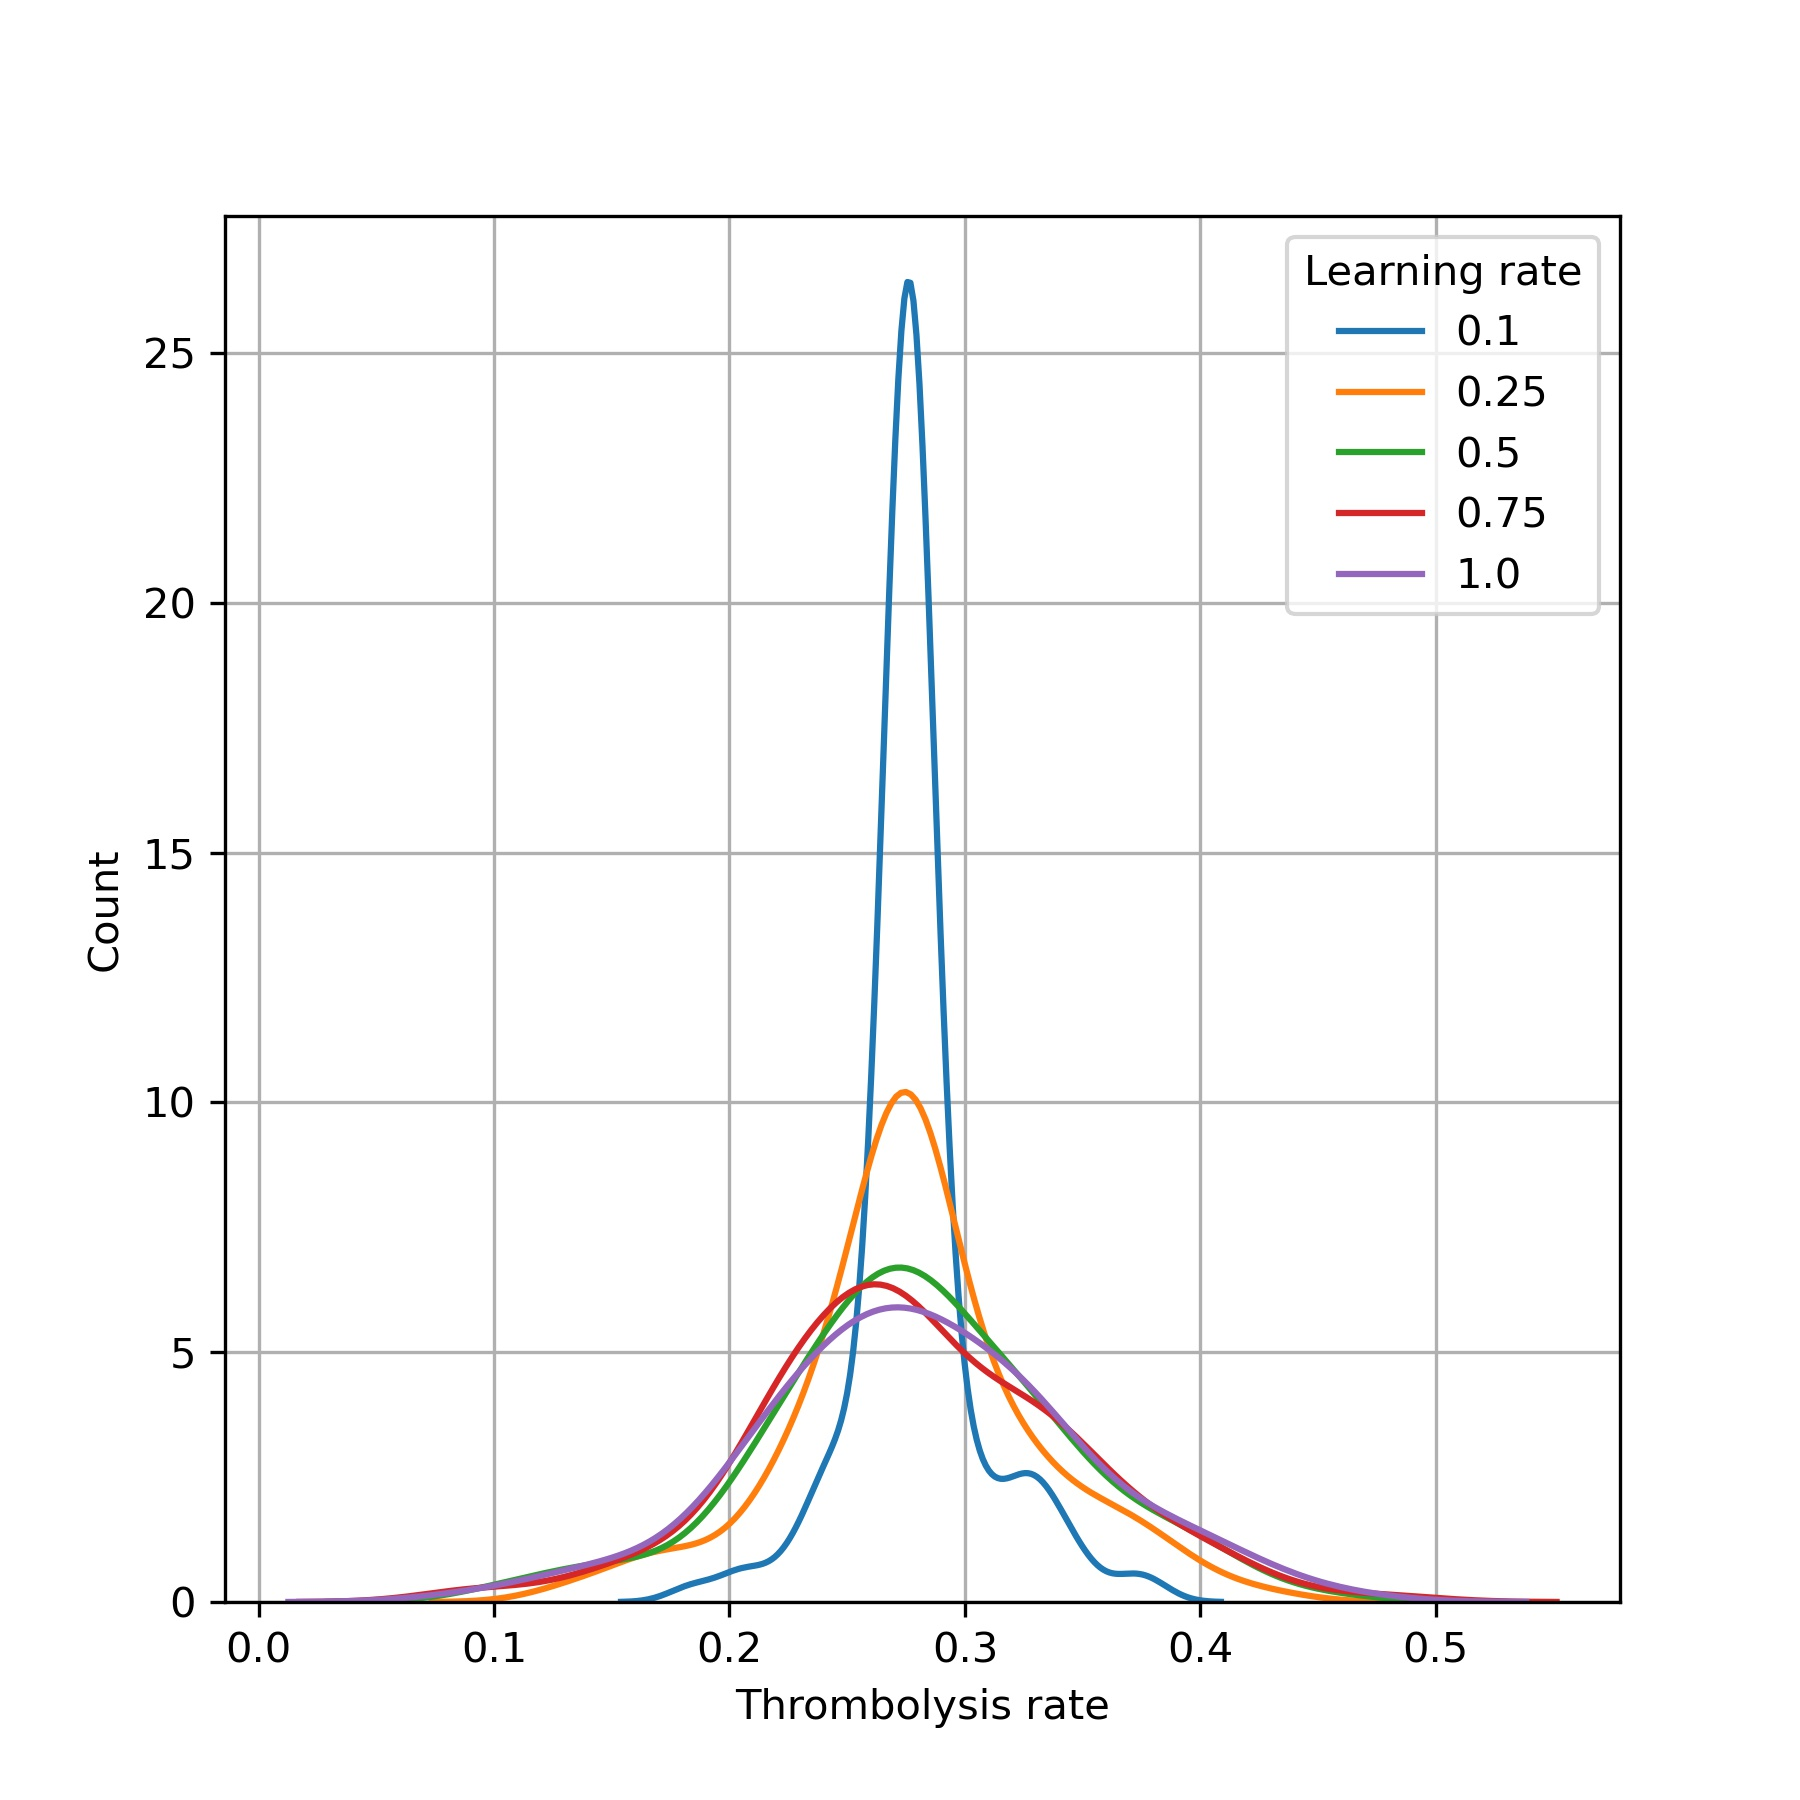
\includegraphics[width=0.7\textwidth]{./images/91_learning_rate}
\caption{Effect of adjusting XGBoost learning rate on the distribution predicted thrombolysis use across 132 hospitals. A narrower distribution indicates that hospital thrombolysis rates are tending towards the mean thrombolysis hospital rate.}
\label{fig:learning_rate}
\end{figure}

\begin{minipage}{\textwidth}
\begin{longtable}[]{@{}llllll@{}}
\caption{Statistics on the variation in predicted thrombolysis use between hospitals, with varying learning rate}\\
\toprule
Learning rate & 0.1 & 0.25 & 0.5 & 0.75 & 1.0\tabularnewline
\midrule
\endhead
Mean & 0.28 & 0.28 & 0.28 & 0.28 & 0.28\tabularnewline
StdDev & 0.03 & 0.05 & 0.06 & 0.07 & 0.07\tabularnewline
Min & 0.18 & 0.13 & 0.10 & 0.09 & 0.09\tabularnewline
Max & 0.38 & 0.43 & 0.45 & 0.48 & 0.46\tabularnewline
\bottomrule
\label{tab:learning_rate}
\end{longtable}
\end{minipage}
%%%%%%%%%%%%%%%%%%%%%%%%%%%%%%%%%%%%%%%%%%%%%%%%%%%%%%%%%%%%%%%%%%%%%%%%%%%%%%%%%%%%%%%

\iffalse

\subsection{An analysis of the characteristics of the most thrombolysable patient at each hospital}

We identified the patient with the highest probability of thrombolysis (taken from 5-fold combined test set results) at each hospital, and compared the feature values of those patients to:

\begin{itemize}
\item All patients
\item All patients who had received thrombolysis
\item All patients who had not received thrombolysis
\end{itemize}

As shown in figure \ref{fig:most_thrombolysable}, compared with the other groups, the most thrombolysable patients:
\begin{itemize}
\item Had shorter arrrival-to-scan times
\item Had an infarction stroke type
\item Had stroke servities with NIHR 5-25
\item Had a precise onset time
\item Had lower pre-stroke disability
\item Were not taking anticoagulant medication
\item Had shorter onset-to-arrival times
\item Did not have onset during sleep
\item Were younger
\end{itemize}

\begin{figure}
\centering
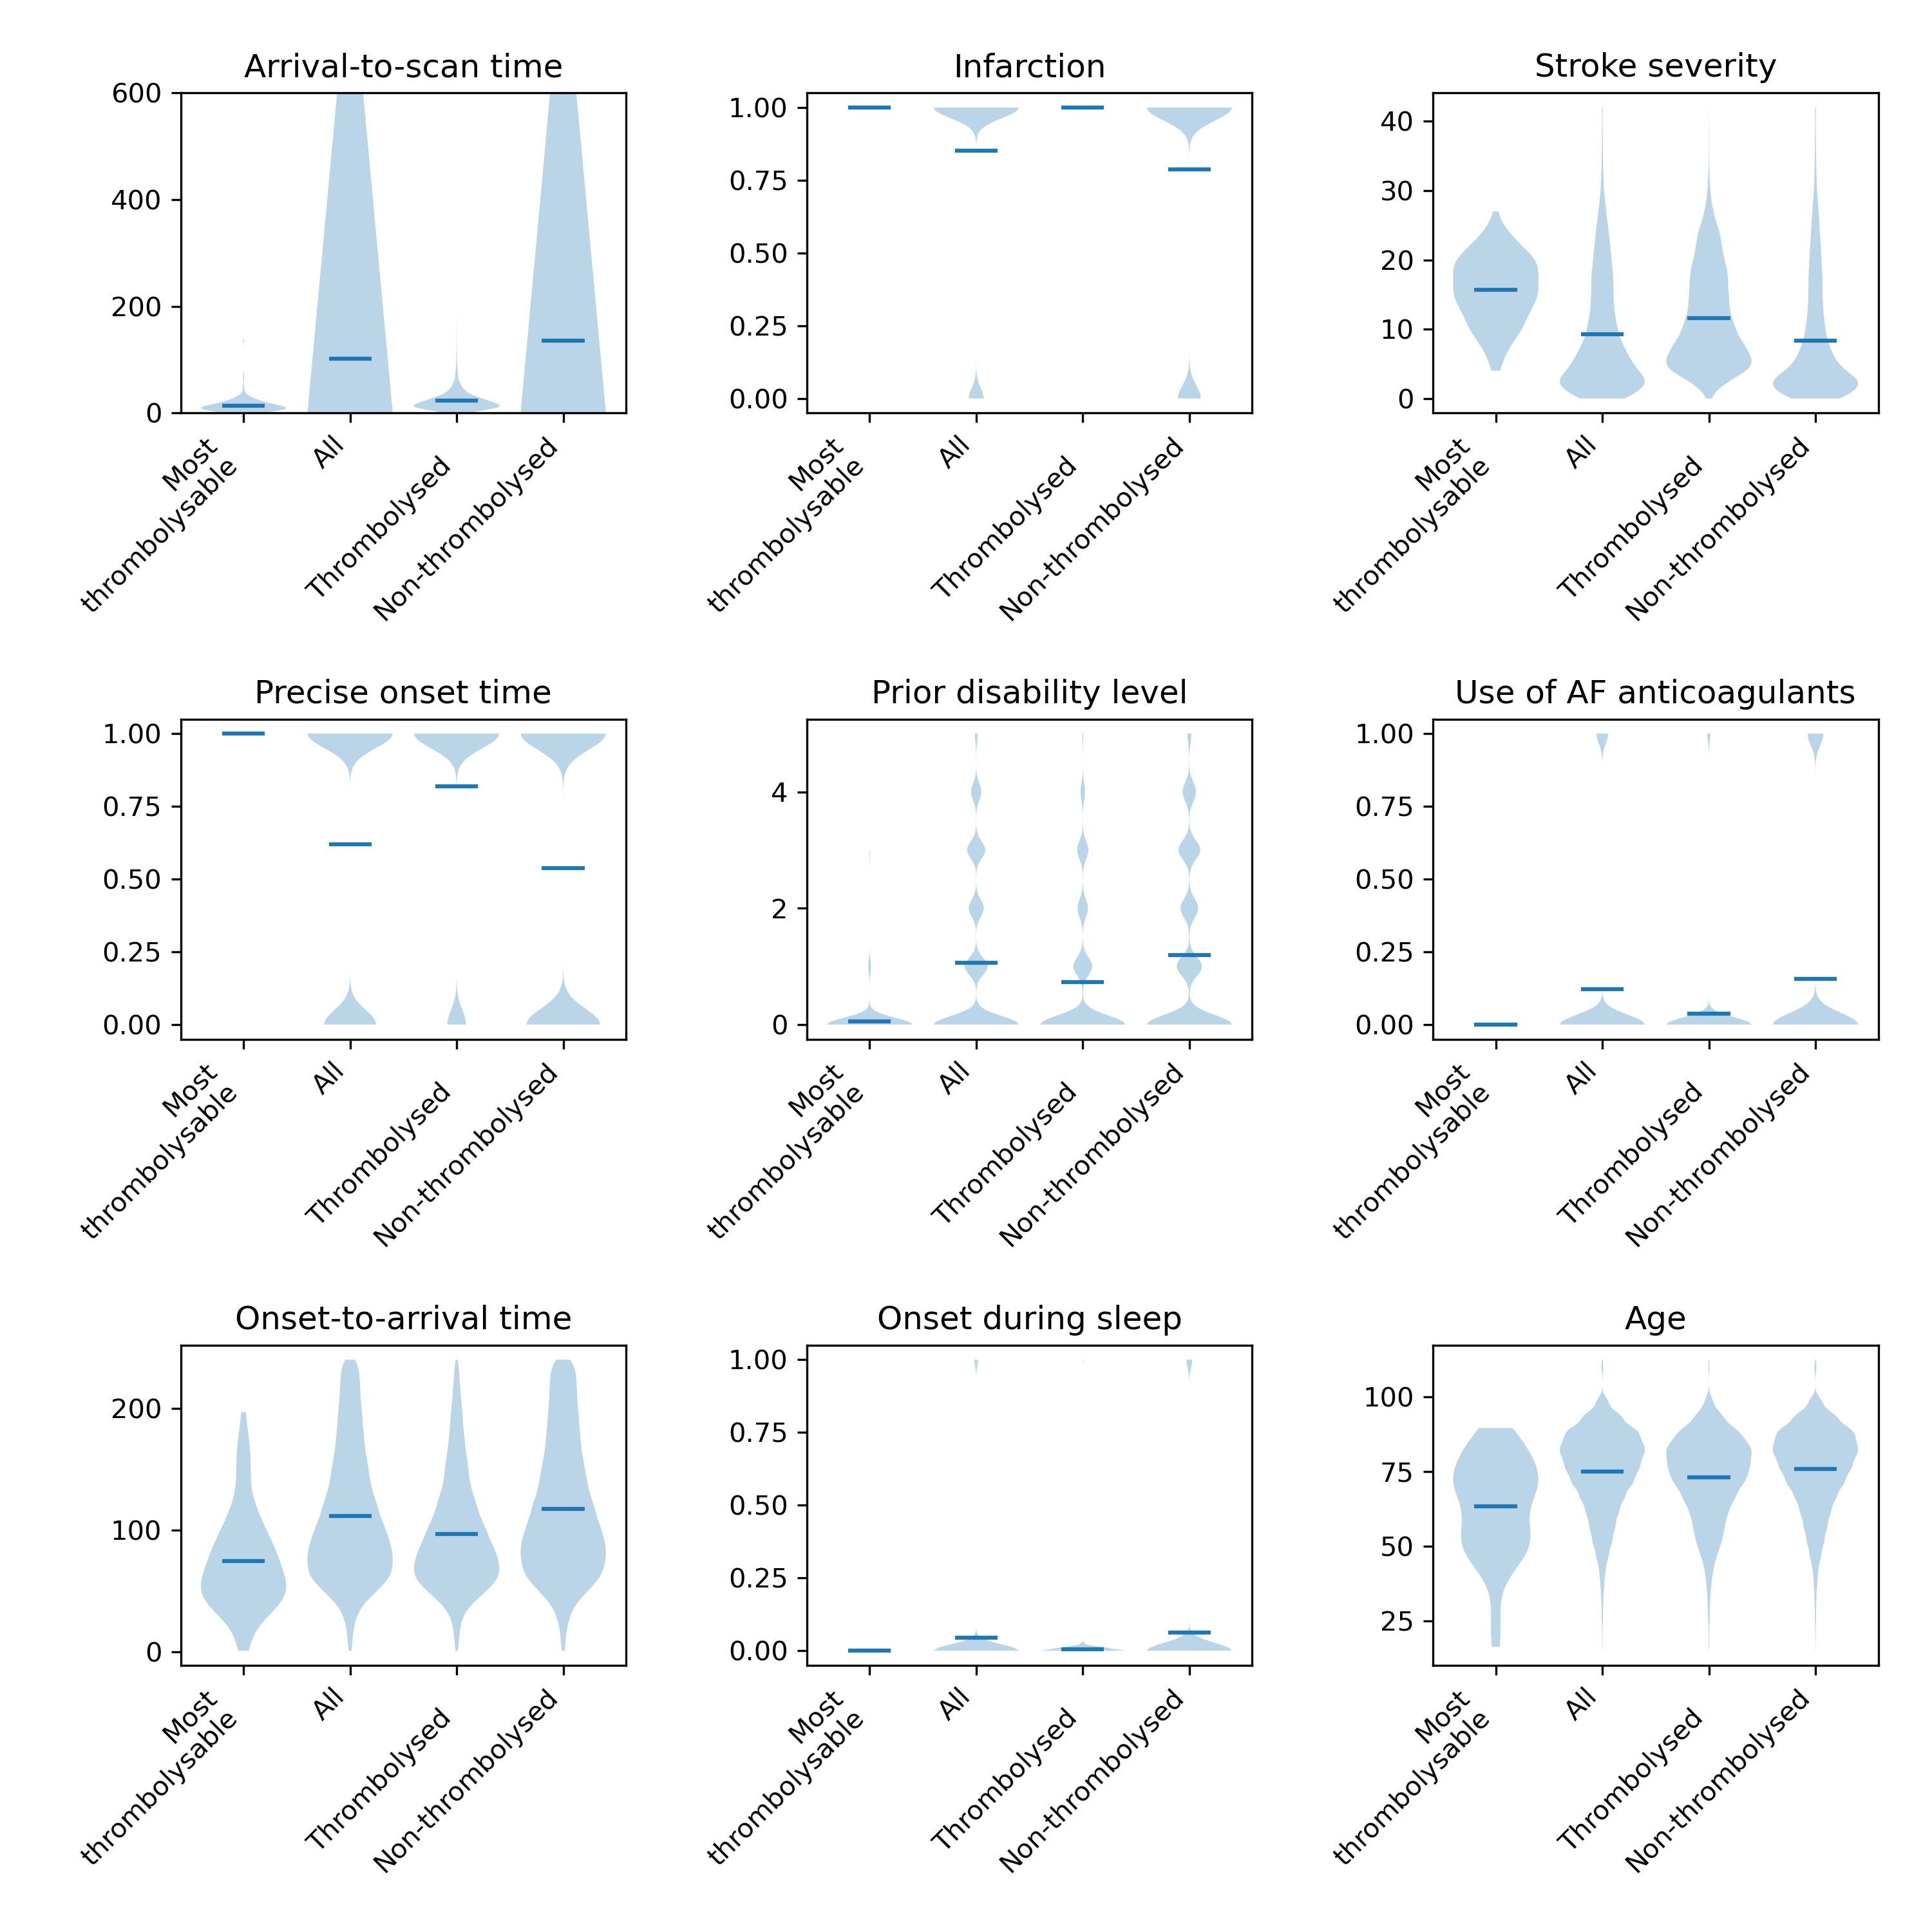
\includegraphics[width=1\textwidth]{./images/02a_most_thrombolsyable_violin}
\caption{Violin plots comparing feature values between the patient with the highest probability of thrombolysis at each hospital with all patients, all patients who had received thrombolysis, and all patients who had not received thrombolysis. Horizontal blue lines show the mean value of each group.}
\label{fig:most_thrombolysable}
\end{figure}

%%%%%%%%%%%%%%%%%%%%%%%%%%%%%%%%%%%%%%%%%%%%%%%%%%%%%%%%%%%%%%%%%%%%%%%%%%%%%%%%%%%%%%%

\subsection{Explaining model predictions with SHAP}

SHAP values describe how much a feature affects the probability of receiving thrombolysis. These are usually expressed as log odds.

%%%%%%%%%%%%%%%%%%%%%%%%%%%%%%%%%%%%%%%%%%%%%%%%%%%%%%%%%%%%%%%%%%%%%%%%%%%%%%%%%%%%%%%

\subsubsection{Waterfall plots for individual patient predictions}

Waterfall plots show the influence of features for an individual prediction. We generally handle SHAP values as how they affect log odds of receiving thrombolysis, but for individual predictions, probability plots are more intuitive for many people to follow. The example shown in figure \ref{fig:waterfall_low}is for a patient with a low probability of receiving thrombolysis. The model started with a base prediction of a 24\% probability of receiving thrombolysis, before feature values are taken into account. Some features (coloured red) increased that base probability of receiving thrombolysis; those were onet-to-arrival time, having a precise onset time, having no prior disability, and being young. Three features (shown in blue) reduced the probability of receiving thrombolysis: the hospital they attended, the long arrival-to-scan time, and having a mild stroke, with a resulting final probability of receiving thrombolysis of 3\%.

\begin{figure}
\centering
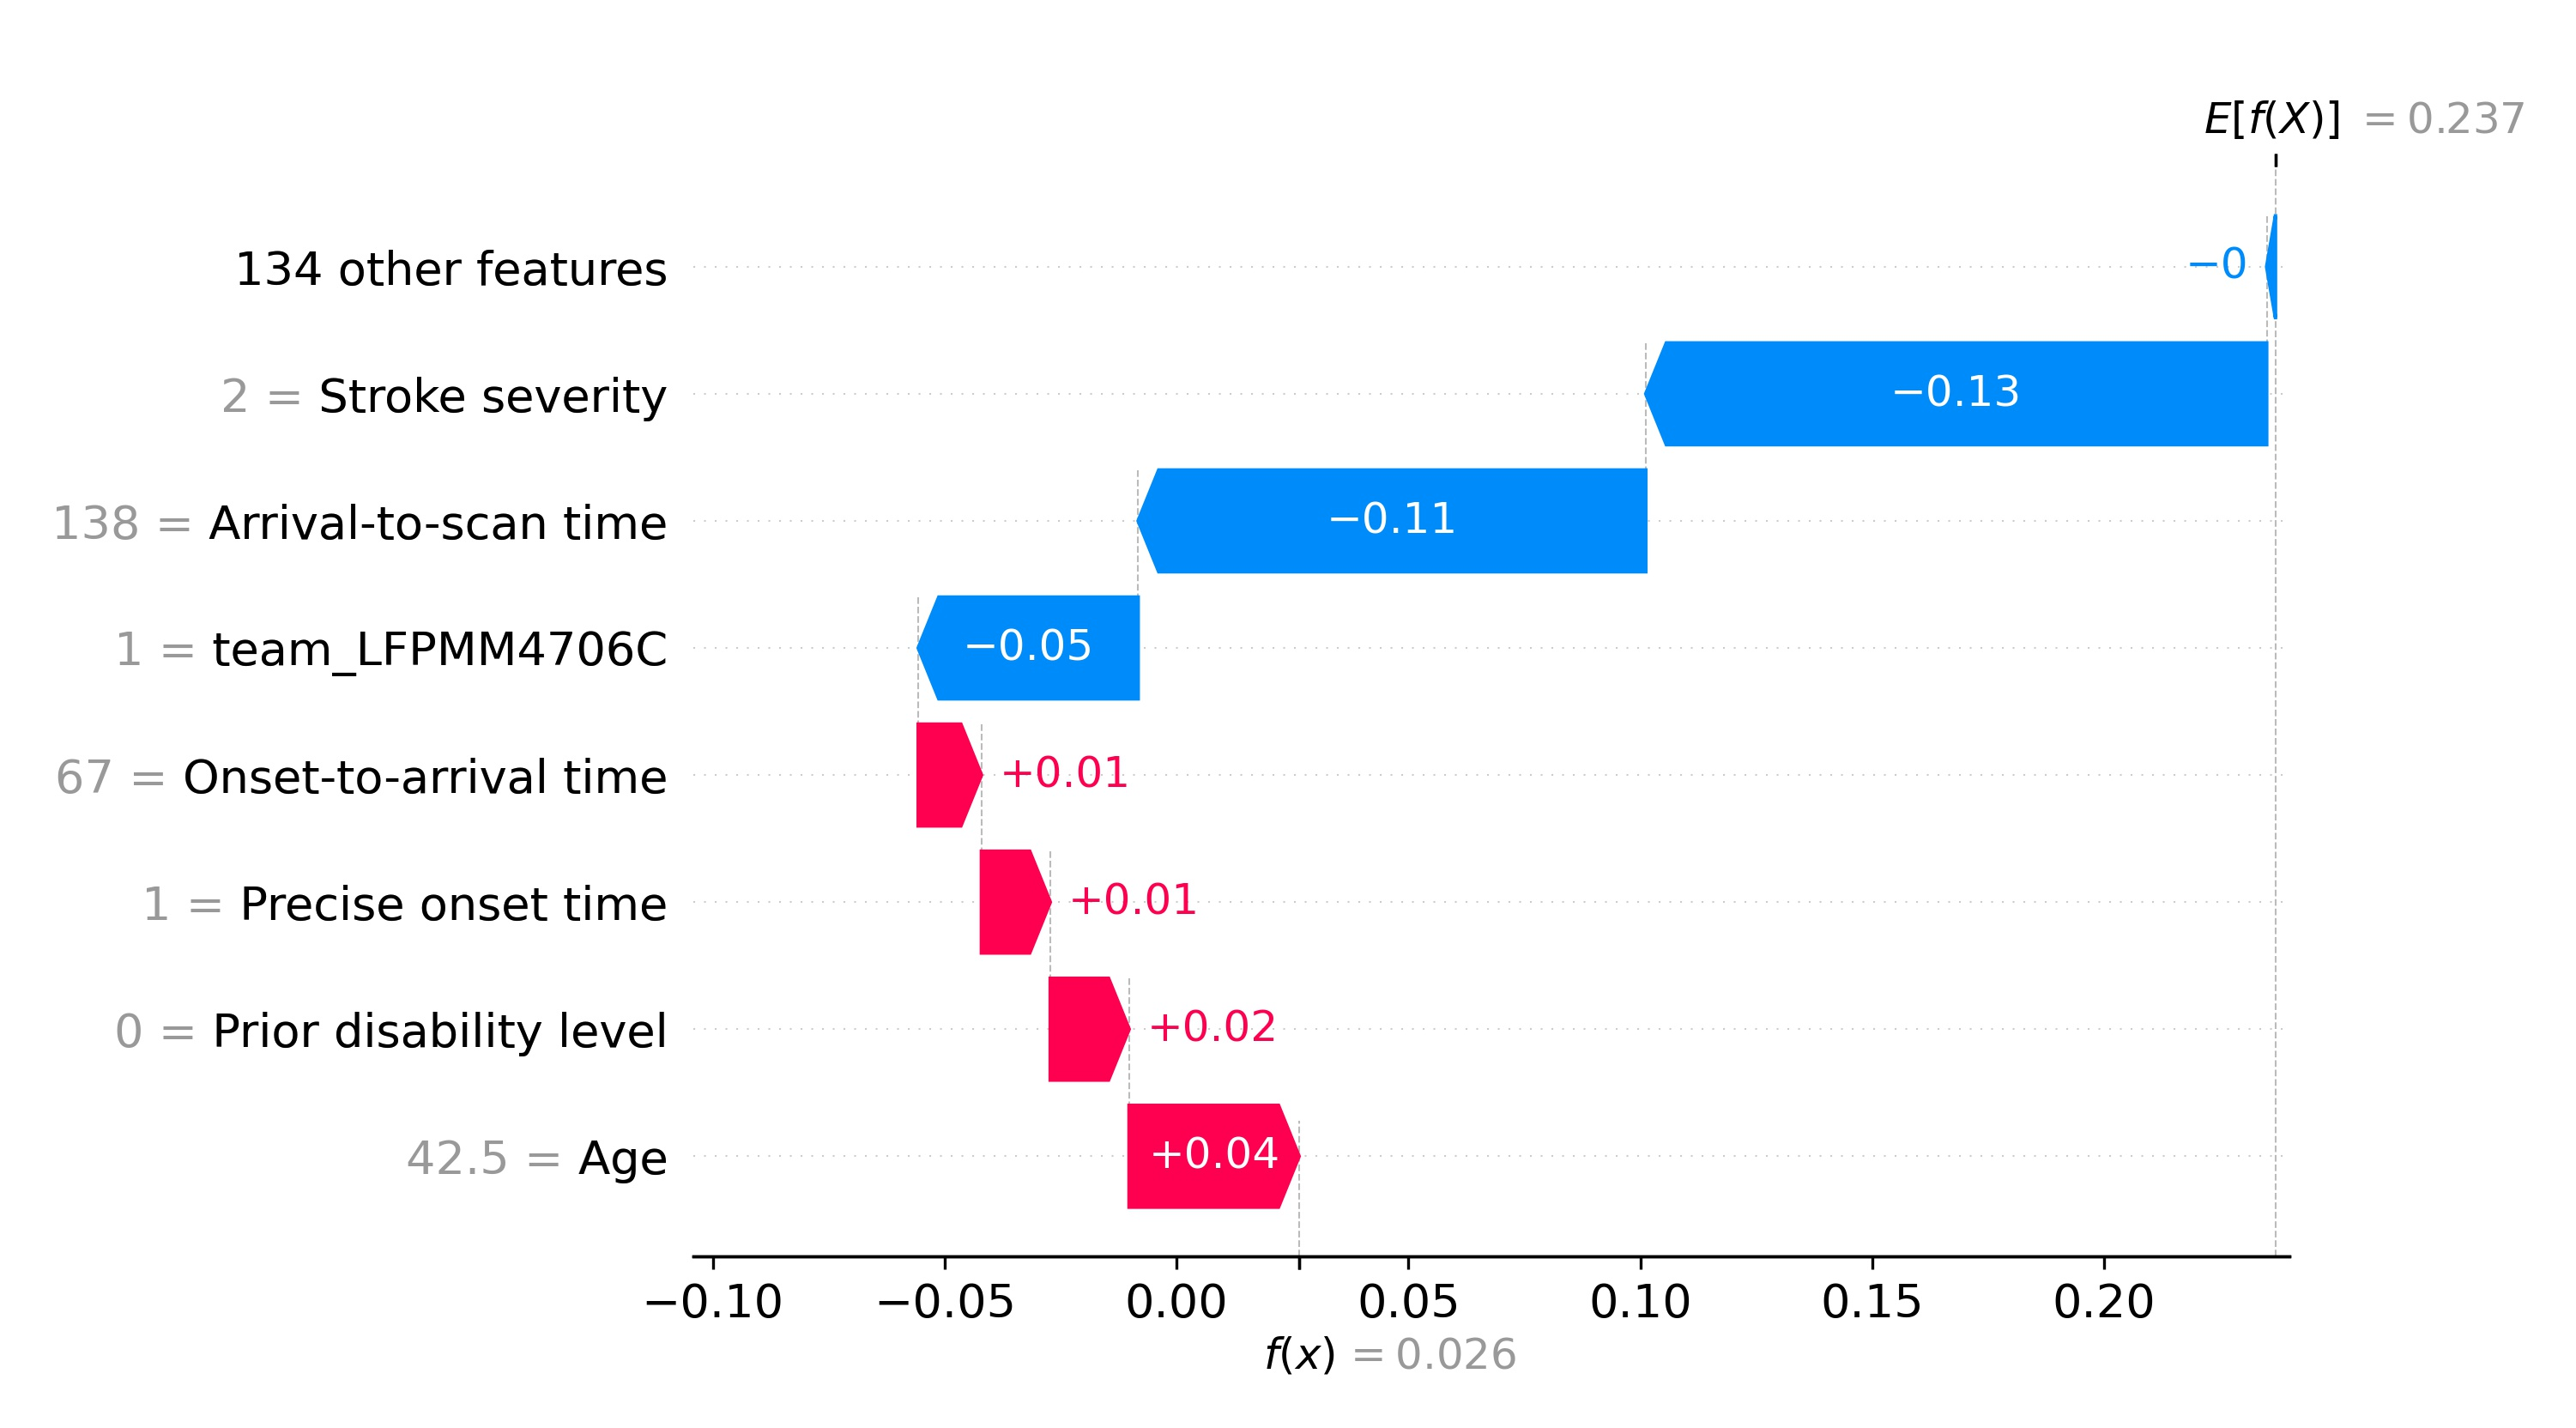
\includegraphics[width=0.85\textwidth]{./images/03_xgb_10_features_waterfall_probability_low}
\caption{Waterfall plot showing the influence of each feature on the predicted probability of a single patient receiving thrombolysis. This example is for a patient with a predicted low probability of receiving thrombolysis.}
\label{fig:waterfall_low}
\end{figure}

Figure \ref{fig:waterfall_high} a similar plot for a patient with a high (96\%) probability of receiving thrombolysis.

\begin{figure}
\centering
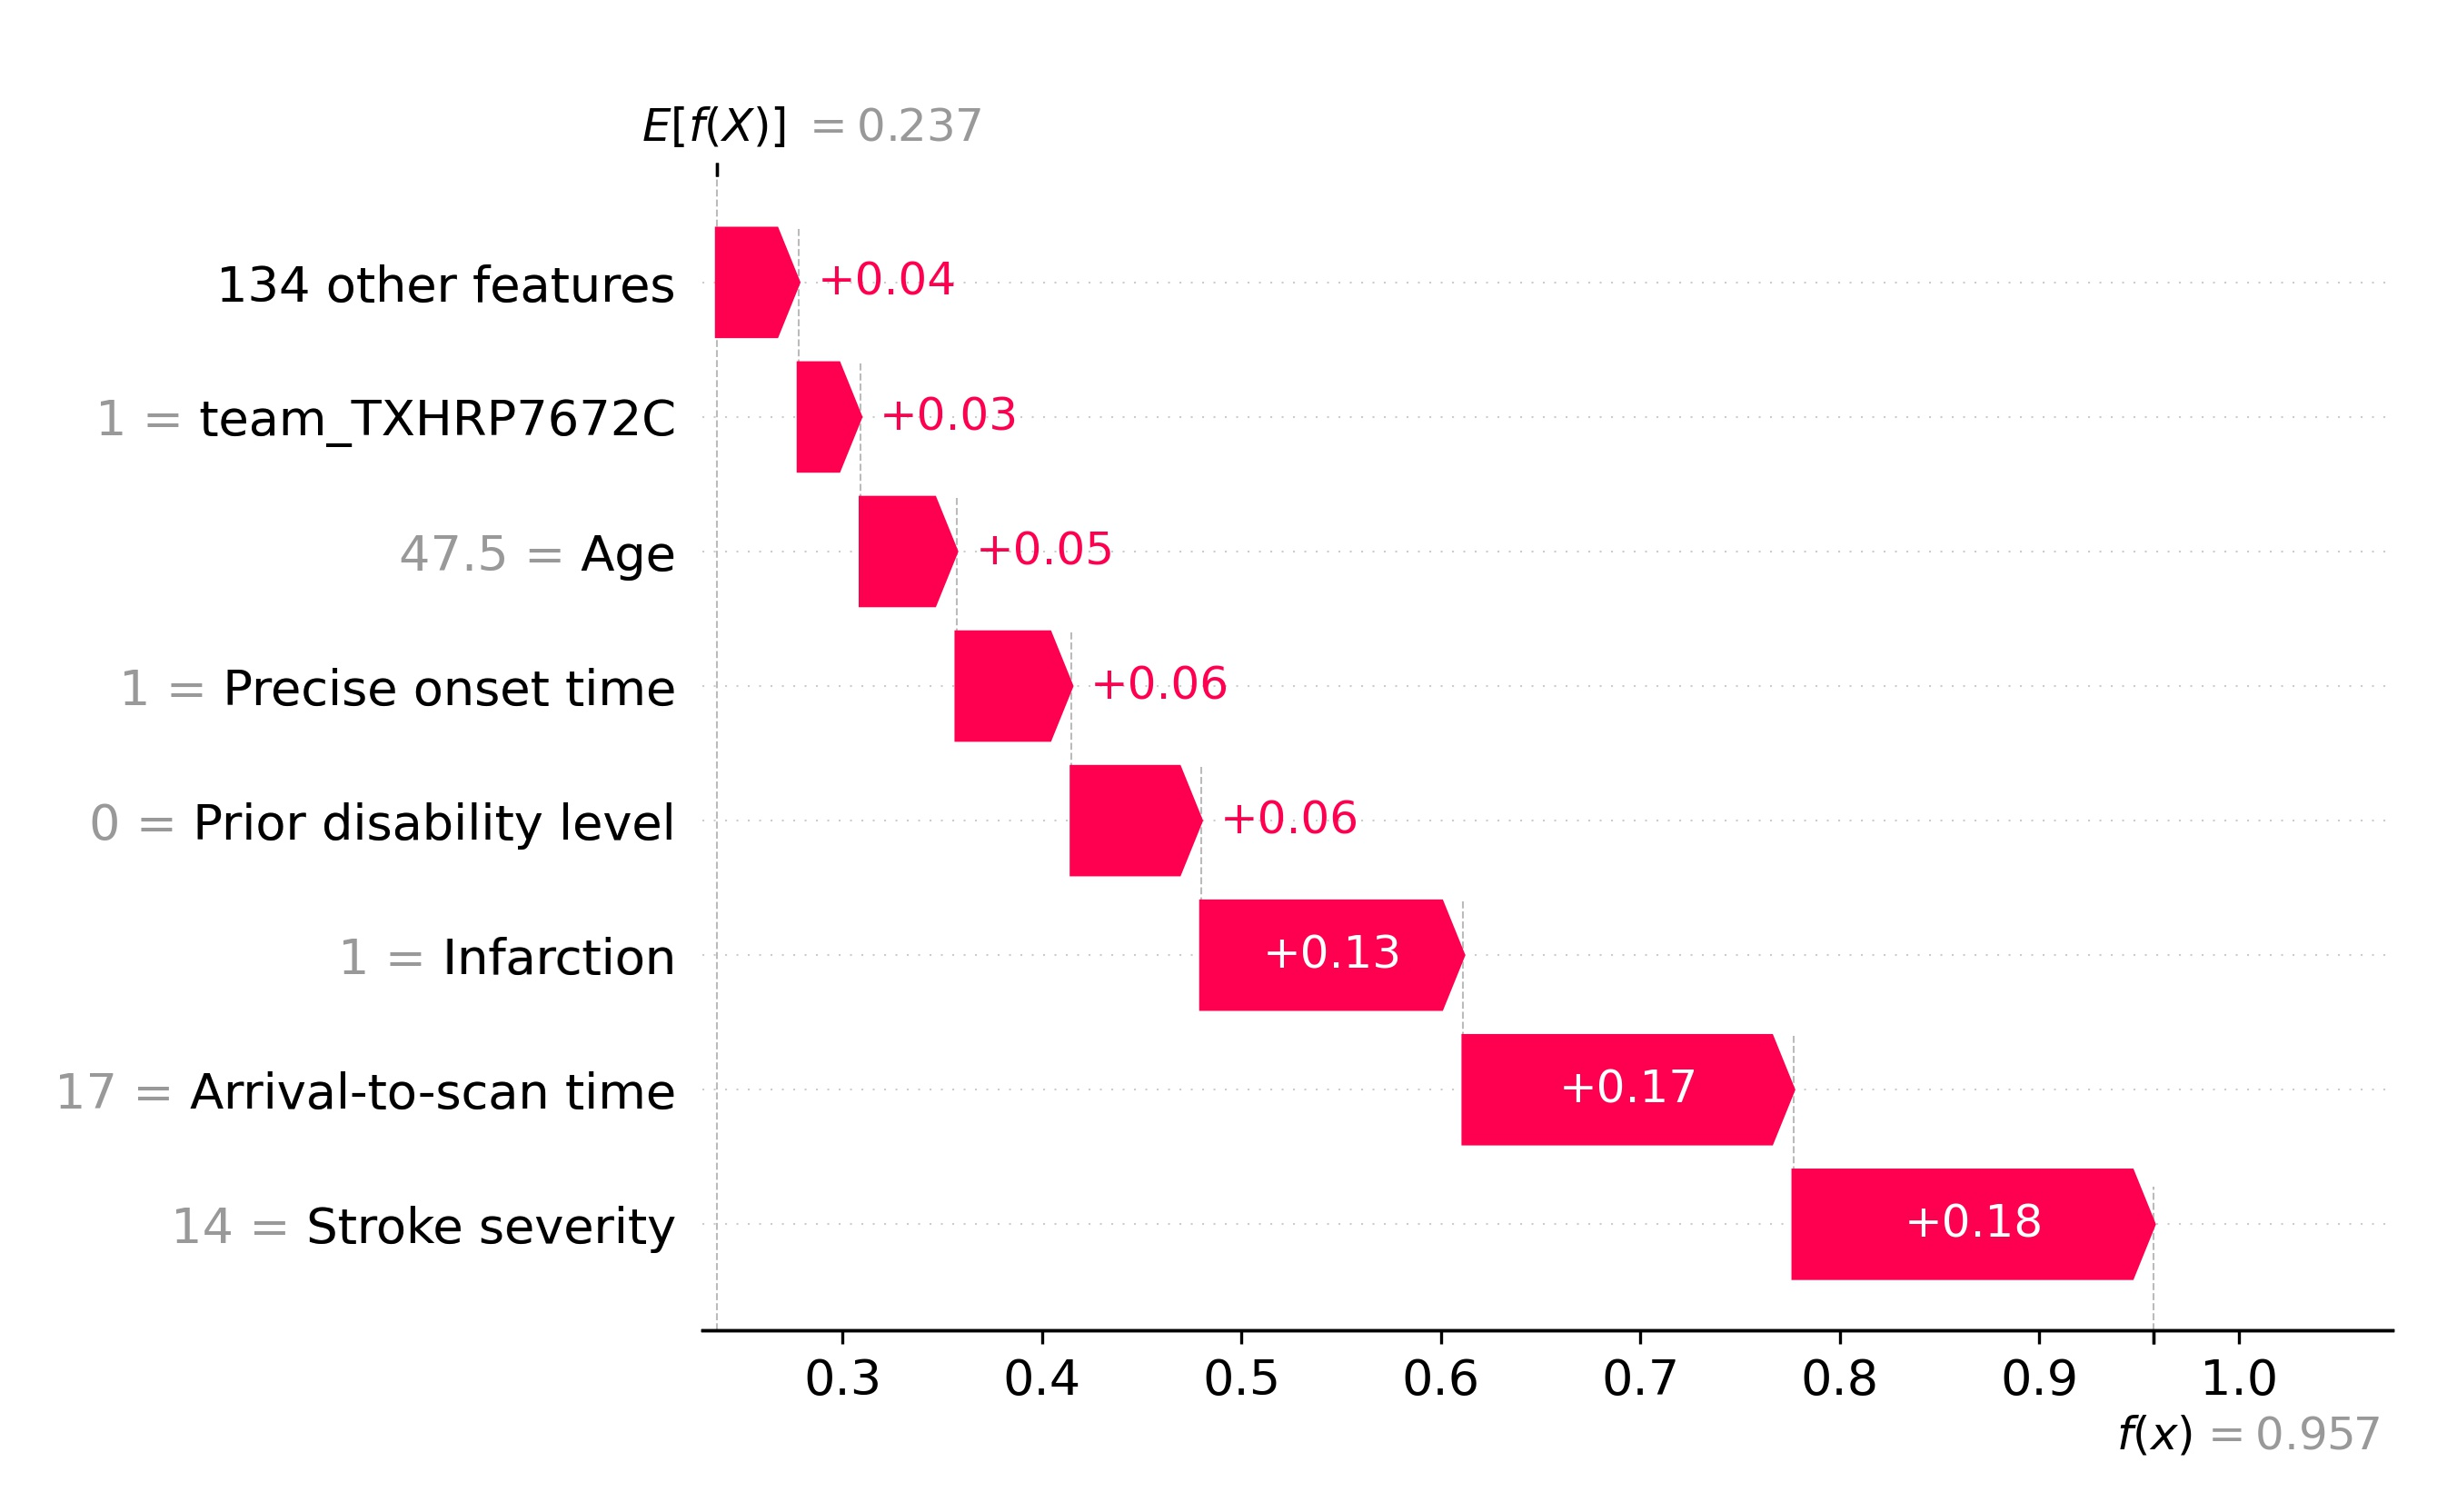
\includegraphics[width=0.85\textwidth]{./images/03_xgb_10_features_waterfall_probability_high}
\caption{Waterfall plot showing the influence of each feature on the predicted probability of a single patient receiving thrombolysis. This example is for a patient with a predicted high probability of receiving thrombolysis.}
\label{fig:waterfall_high}
\end{figure}

\subsubsection{Consistency of SHAP values across 5-fold validation}

We examined how reproducible SHAP values are between different k-fold models (figure \ref{fig:shap_consistency}. The figure below shows the variation in mean absolute SHAP values obtained from the training sets of the 5 models in k-fold validation. SHAP values are well maintained across the five models.

\begin{figure}
\centering
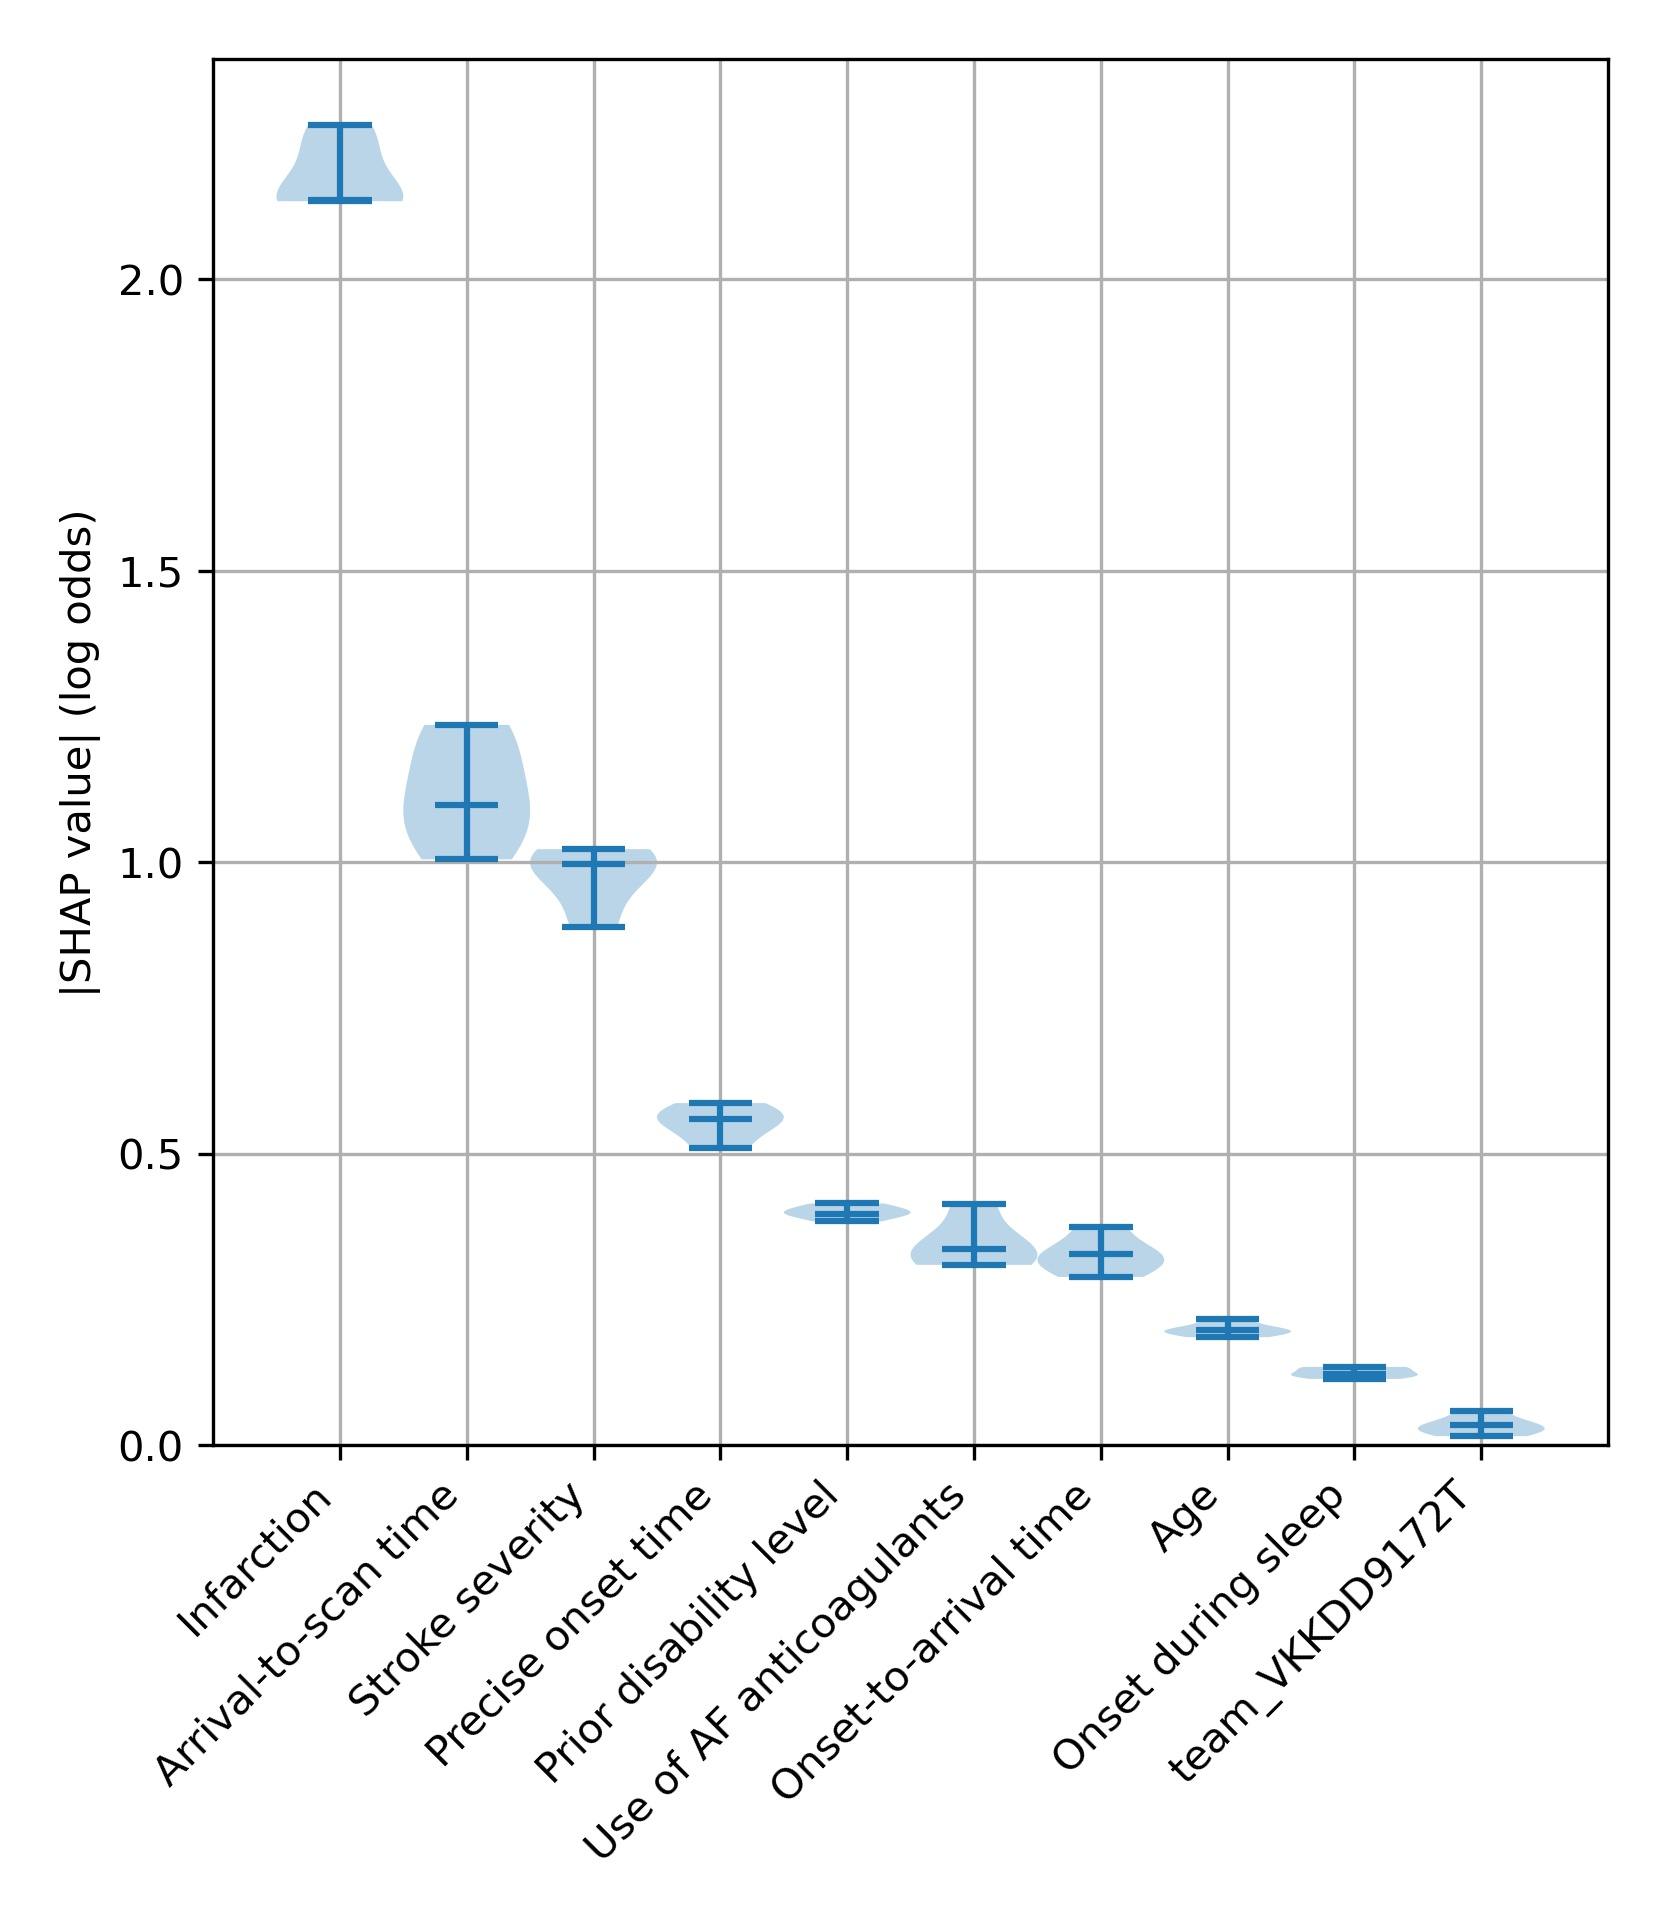
\includegraphics[width=0.7\textwidth]{./images/03_xgb_10_features_shap_violin}
\caption{Violin plots show the distribution of SHAP values across 5 k-fold models. The horizontal bar shows the median absolute SHAP value.}
\label{fig:shap_consistency}
\end{figure}

We also saw the order of general influence of features across the population (note: teams were separated out into individual one-hot features, and needed a separate analysis to examine SHAP of only those patients attending a particular hospital, as otherwise the SHAP was dominated by all the '0' one-hot encoded feature values):

\begin{enumerate}
\item Infarction
\item Arrival-to-scan time
\item Stroke severity
\item Precise onset time
\item Prior disability level
\item Use of AF anticoagulants
\item Onset-to-arrival time
\item Age
\item Onset during sleep
\end{enumerate}

%%%%%%%%%%%%%%%%%%%%%%%%%%%%%%%%%%%%%%%%%%%%%%%%%%%%%%%%%%%%%%%%%%%%%%%%%%%%%%%%%%%%%%%

\subsubsection{Beeswarm plot of SHAP values}

The \emph{beeswarm} plot gives a high level view of the feature values and SHAP values across the whole data set (figure \ref{fig:beeswarm}. We saw, for example that if a patient had an infarction then SHAP values were in the range 1-2, but if the patient did not have an infarction (i.e. has a haemorrhage) then SHAP values were in the range -8 to -4, effectively preventing the model from ever predicting thrombolysis would be given to a haemorrhagic patient. The beeswarm plot was taken from training set for the first k-fold train/test split.

\begin{figure}
\centering
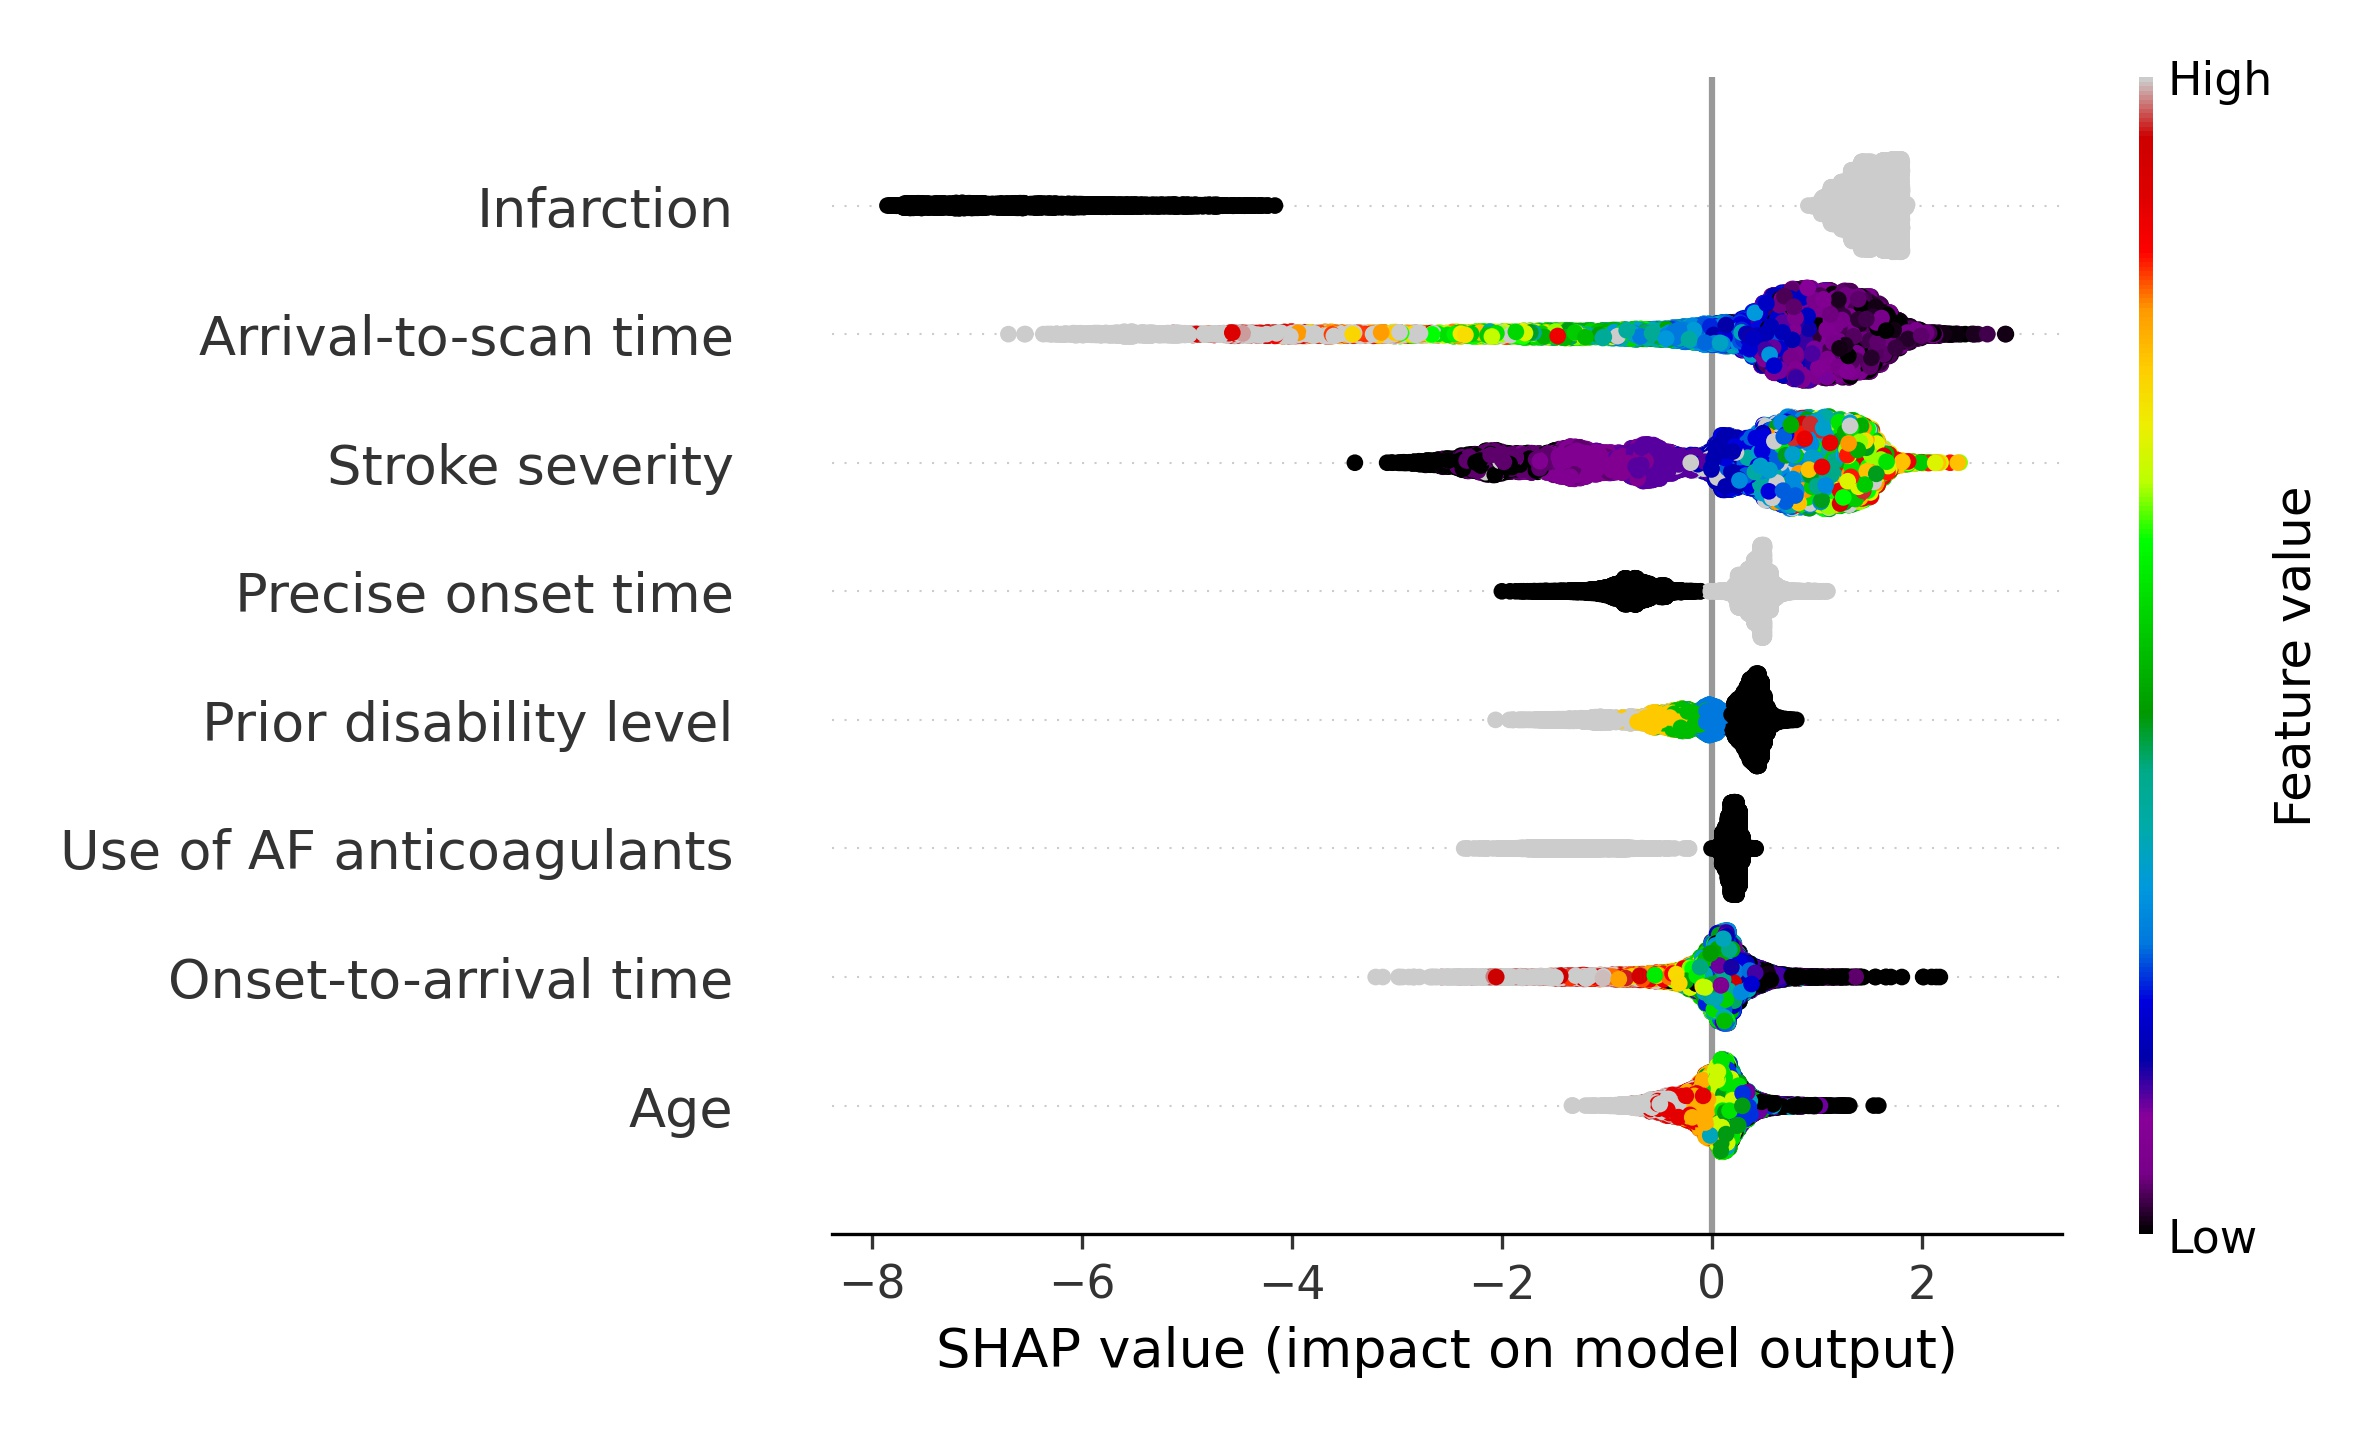
\includegraphics[width=0.8\textwidth]{./images/03_xgb_10_features_beeswarm}
\caption{Beeswarm plot of SHAP values, taken from the training set for the first of 5 k-fold train/test splits. Features values are indicated by color of the points, and the corresponding SHAP value is shown on the x-axis.}
\label{fig:beeswarm}
\end{figure}



%%%%%%%%%%%%%%%%%%%%%%%%%%%%%%%%%%%%%%%%%%%%%%%%%%%%%%%%%%%%%%%%%%%%%%%%%%%%%%%%%%%%%%%

\subsubsection{Violin plots of SHAP values}

Violin plots show the relationship between feature values and SHAP values for individual patients (the bar in each violin shows the median value). The SHAP values were taken the SHAP values of the training set for the first of 5 k-fold train/test splits (figure \ref{fig:shap_violin})..

Note: SHAP values are not necessarily the same for all instances with the same feature value. This is because the SHAP value also depends on interactions between features. For example if a hospital is not pre-disposed to give thrombolysis to patients with mild stroke, the SHAP value for the NIHSS value (e.g. NIHSS=1 for  avery mild stroke) will be lower than the SHAP value for the NIHSS value for a similar patient attending a hospital with a greater predisposition to use thrombolysis in patients with milder strokes. These interactions will be explored later.

\begin{figure}
\centering
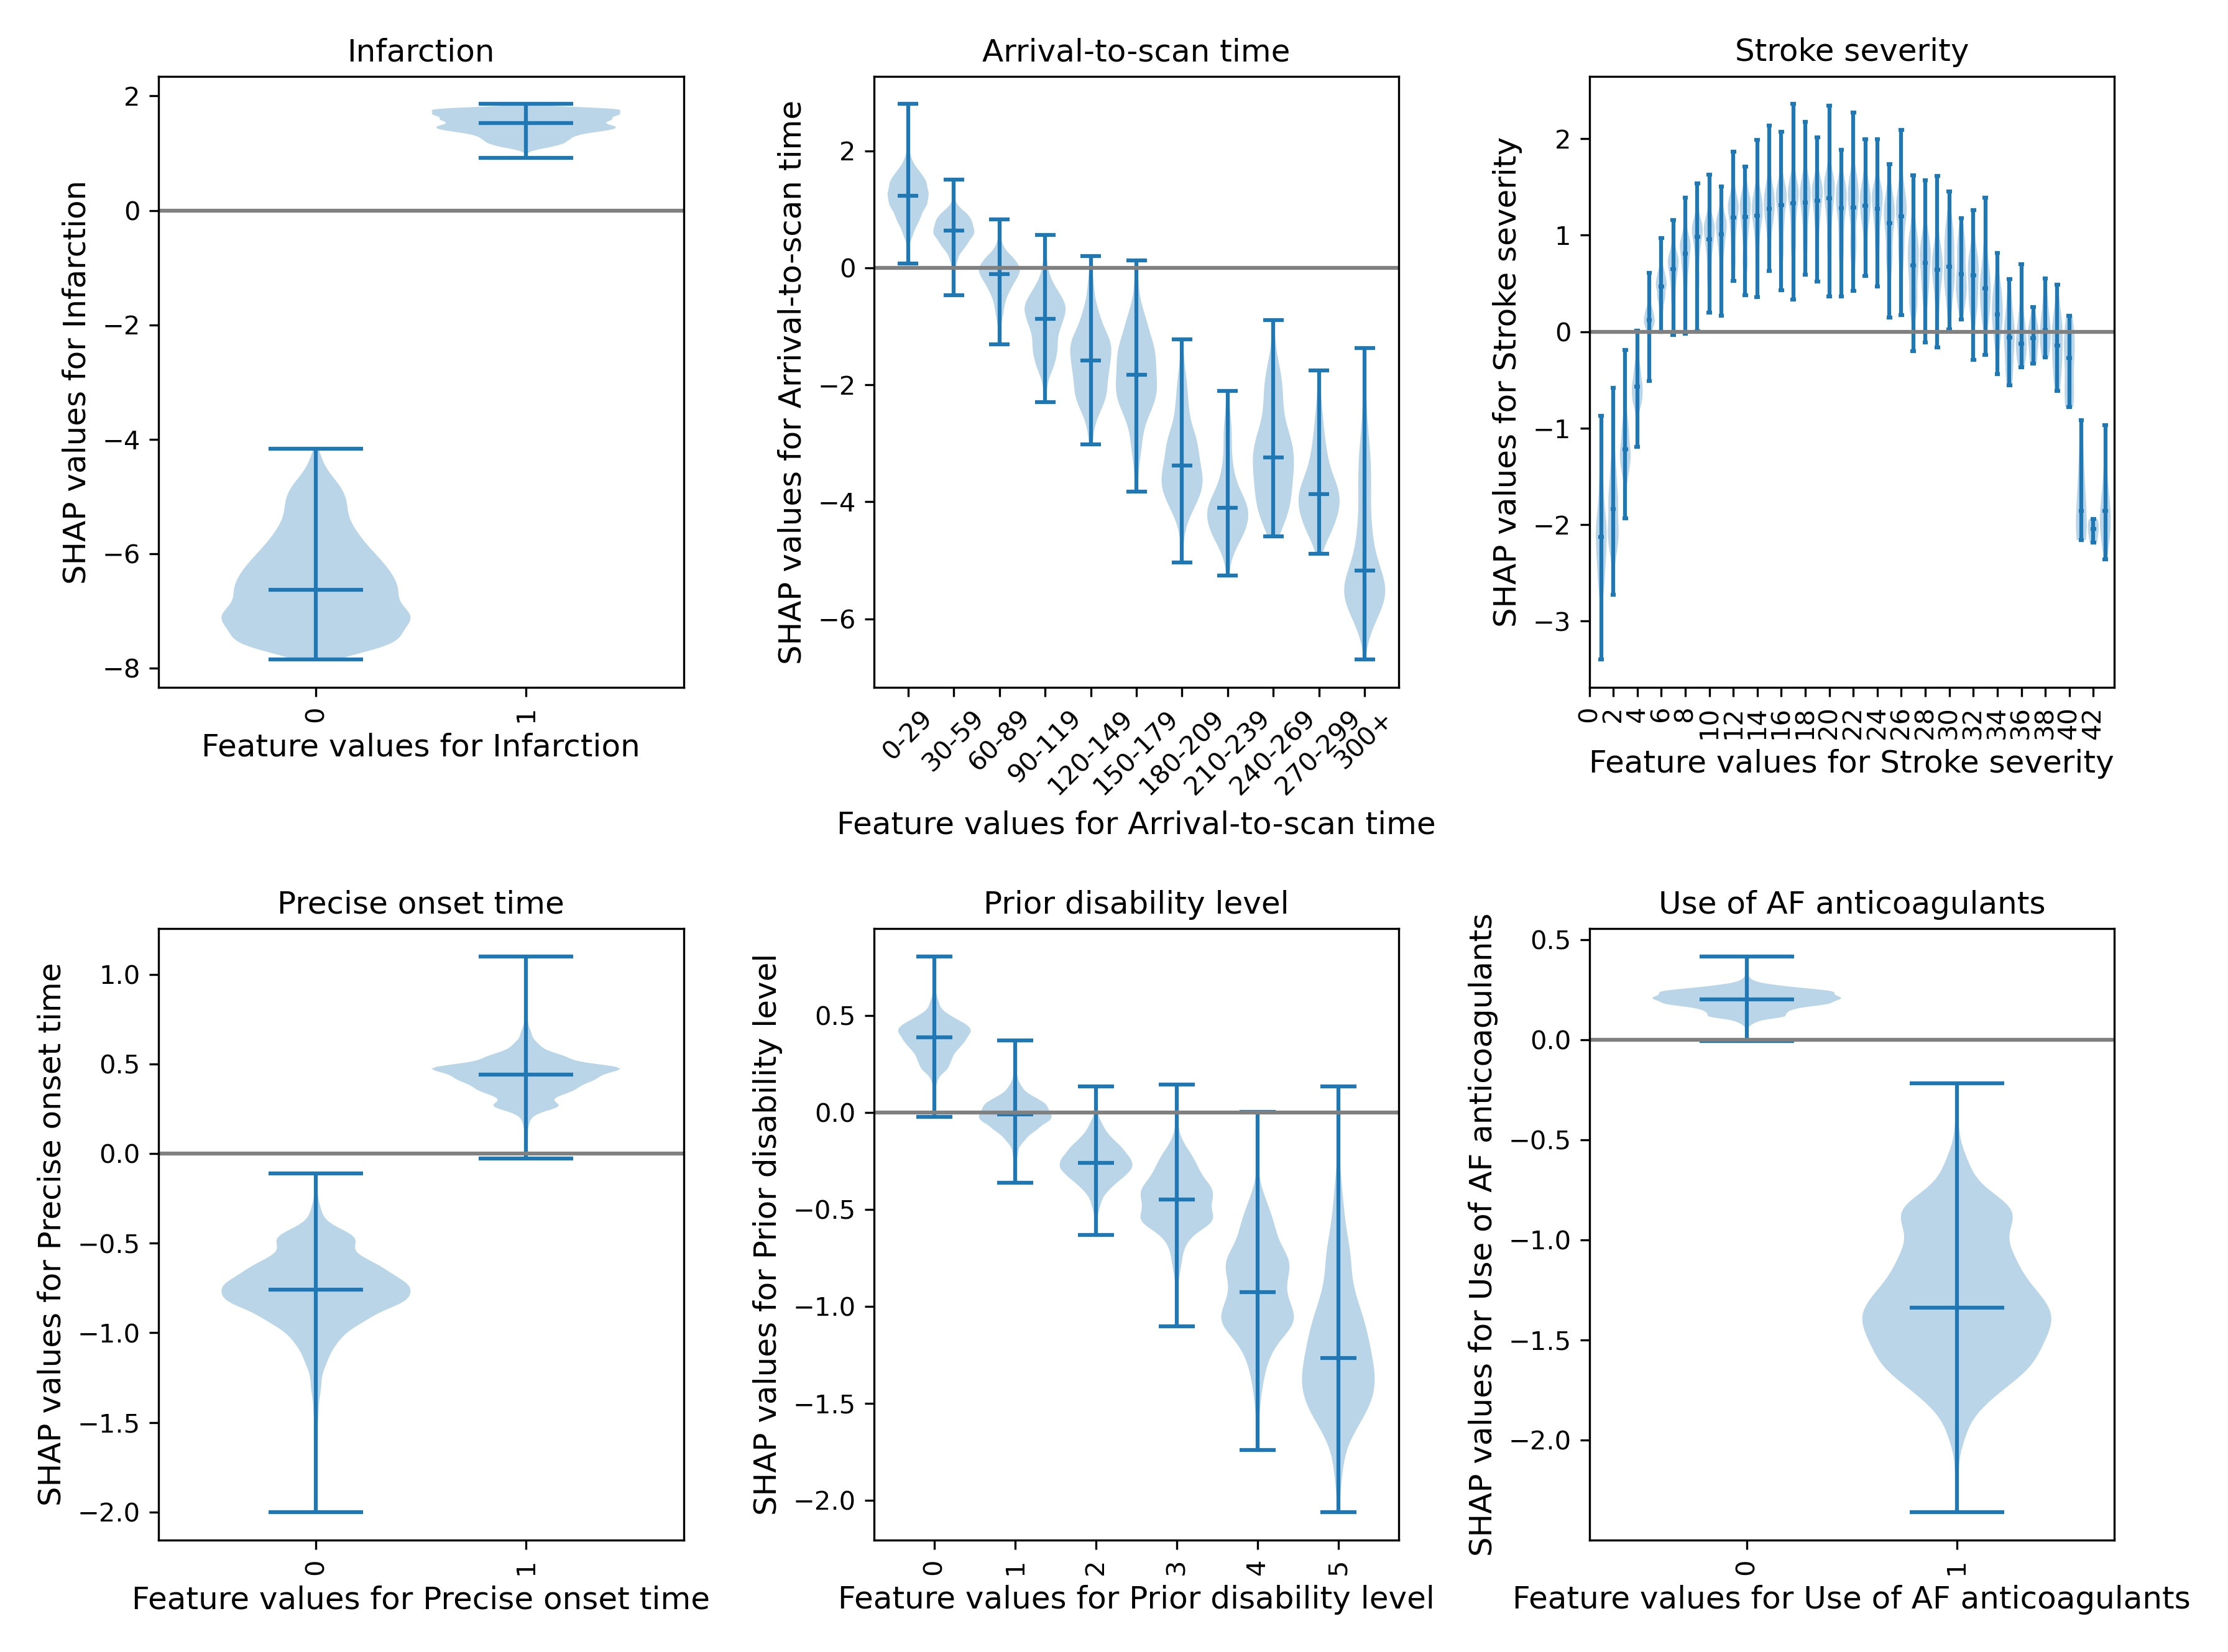
\includegraphics[width=1\textwidth]{./images/03_xgb_10_features_thrombolysis_shap_violin}
\caption{Violin plots showing the relationship between SHAP values and feature values. The horizontal blue lines show the median SHAP value. SHAP values were taken from the training set of the first of 5 k-fold train/test splits.}
\label{fig:shap_violin}
\end{figure}

Key observations were, with SHAP values converted back to odds were:

\begin{itemize}
\item Stroke type: As expected, the SHAP values for stroke types effectively
  eliminated any chance of receiving thrombolysis for non-ischaemic
  (haemorrhagic) stroke.
\item Arrival-to-scan time: The odds of receiving thrombolysis reduced by
  about 20 fold over the first 100 minutes of arrival to scan time.
\item Stroke severity (NIHSS): The odds of receiving thrombolysis was lowest
  at NIHSS 0, rose and peakws at NIHSS 15-25, and then fell again with
  higher stroke severity. The difference between minimum odds (at NIHSS
  0) and maximum odds (at 15-25) of receiving thrombolysis was 30-35
  fold.
\item Stroke onset time type (precise vs.~estimated): The odds of receiving
  thrombolysis were about 3 fold greater for precise onset time than
  estimated onset time.
\item Disability level (Rankin) before stroke. The odds of receiving
  thrombolysis fell about 5 fold between mRS 0 and 5.
\end{itemize}

%%%%%%%%%%%%%%%%%%%%%%%%%%%%%%%%%%%%%%%%%%%%%%%%%%%%%%%%%%%%%%%%%%%%%%%%%%%%%%%%%%%%%%%

\subsubsection{Hospital SHAP values}


When examining SHAP, we took the hospital SHAP values for patients attending each hospital. If we examined the hospital SHAP for all patients, it would be dominated by those not-attending each hospital (i.e. coded zero in the one-hot encoding). When we examined the hospital SHAP values for a model trained on all the data (figure \ref{fig:shap_histogram}), and only for patients attending each hospital, the hospital SHAP values ranged from -1.4 to +1.4. This range of SHAP (log odds) represents a 15 fold difference in odds of receiving thrombolysis (most are in the range of -1 to +1, but this still represents a 7-8 fold difference in odds of receiving thrombolysis). 

\begin{figure}
\centering
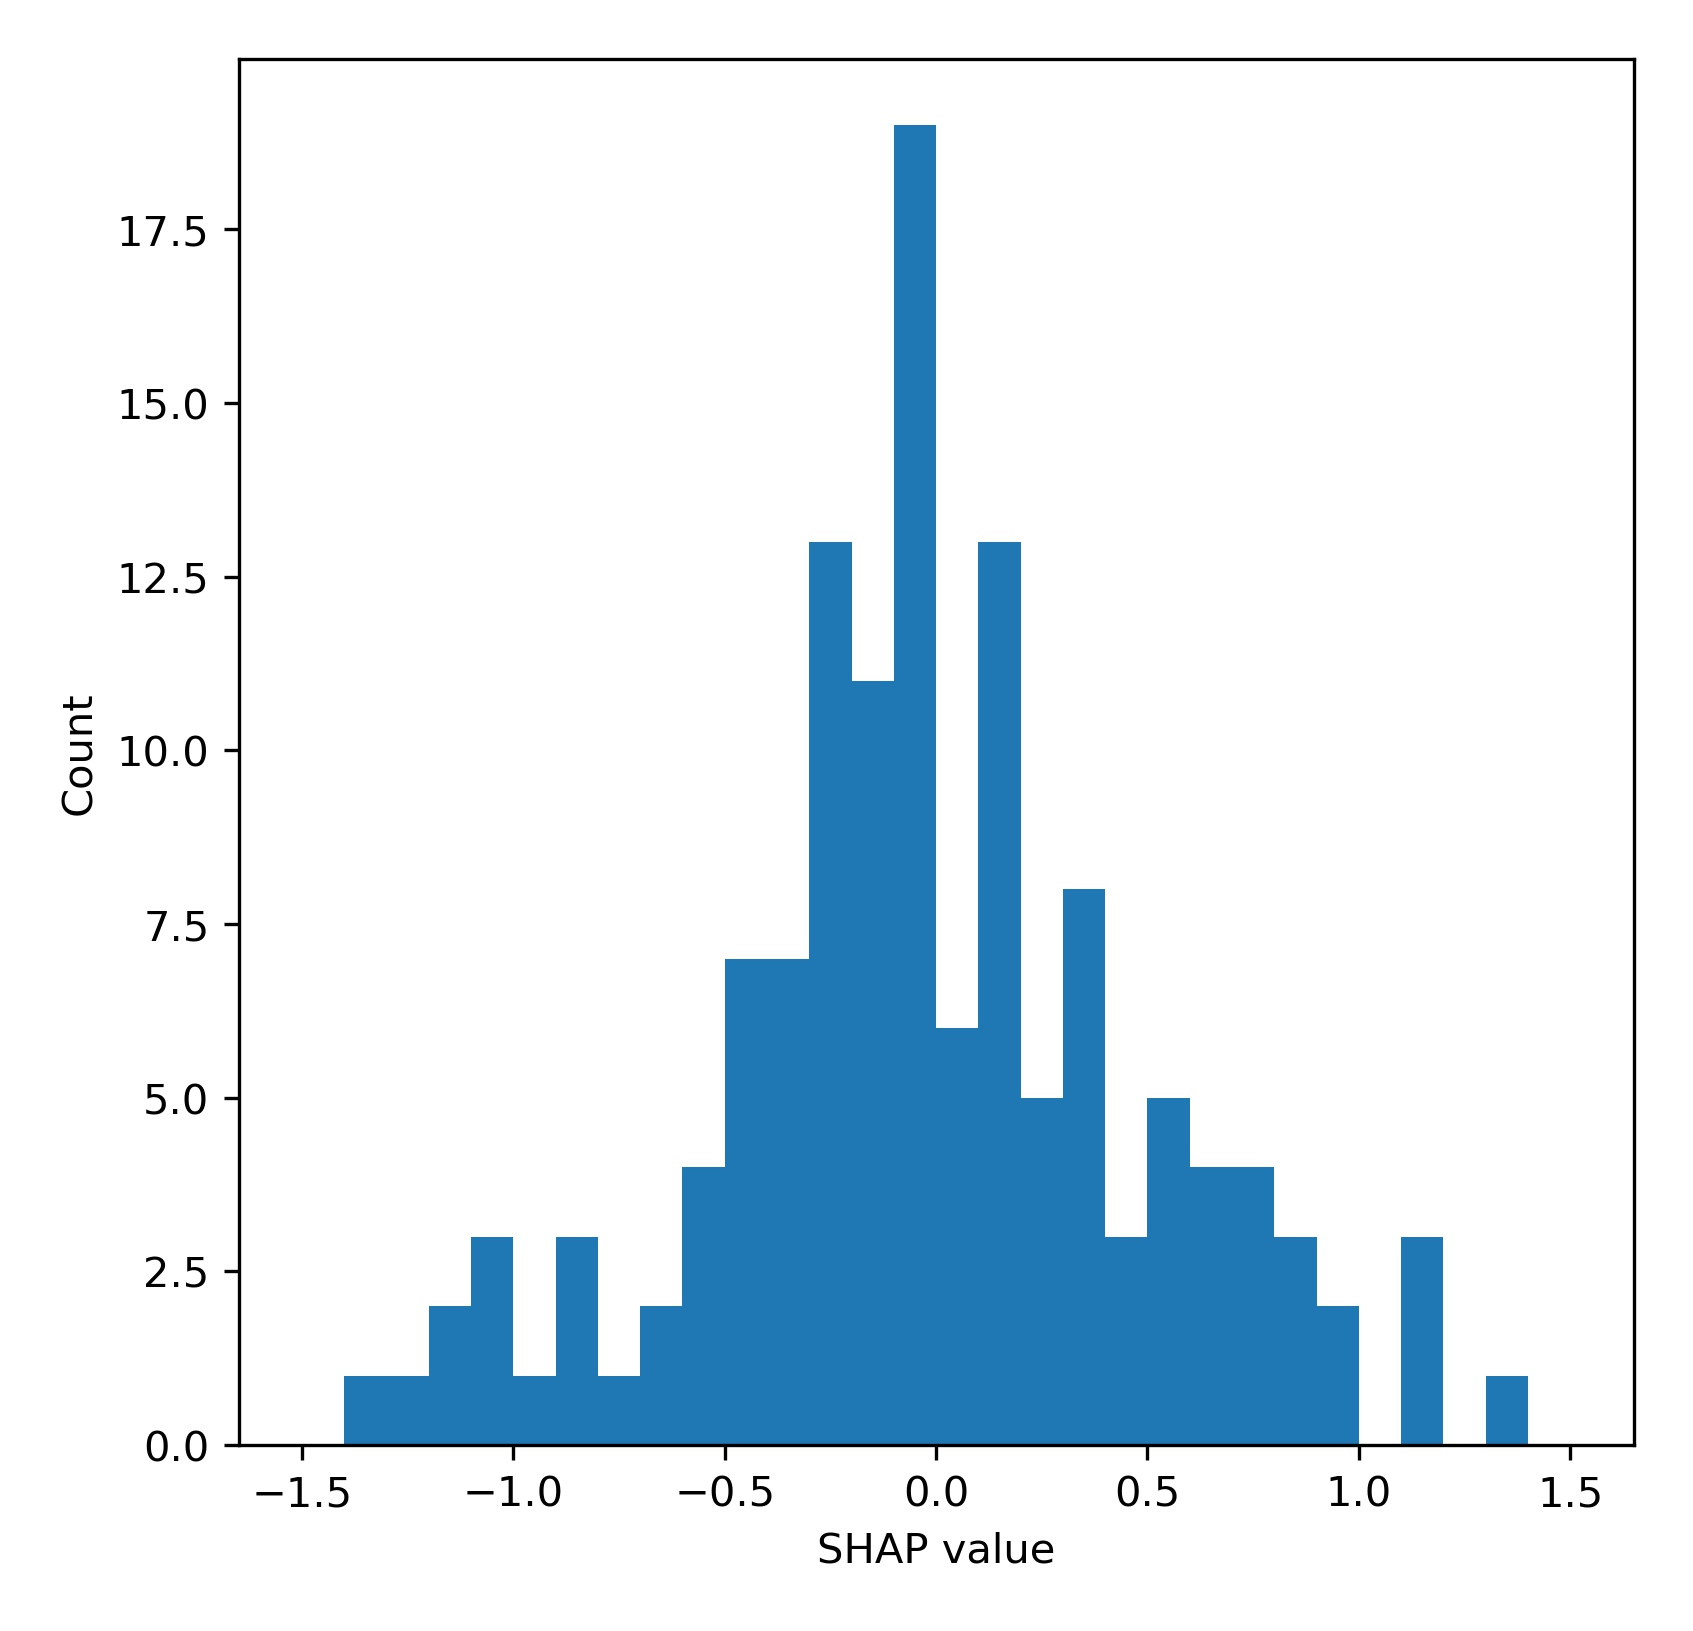
\includegraphics[width=0.7\textwidth]{./images/03_xgb_10_features_hosp_shap_hist}
\caption{Distribution of hospital SHAP values for patients attending each hospital. SHAP values were taken from the training set of the first of 5 k-fold train/test splits.}
\label{fig:shap_histogram}
\end{figure}

We compared the hospital SHAP value with the observed thrombolysis use at each hospital. For this experiment we combined the SHAP values from all the 5 k-fold test data splits, so that all instances were represented.

Hospital SHAP correlated with observed thrombolysis rate with an r-squared of 0.582 (figure \ref{fig:shap_correlation_1}), suggesting that 58\% of the between-hospital variance in thrombolysis use may be explained by the hospitals' SHAP values, that is the hospitals' predisposition to use thrombolysis.

\begin{figure}
\centering
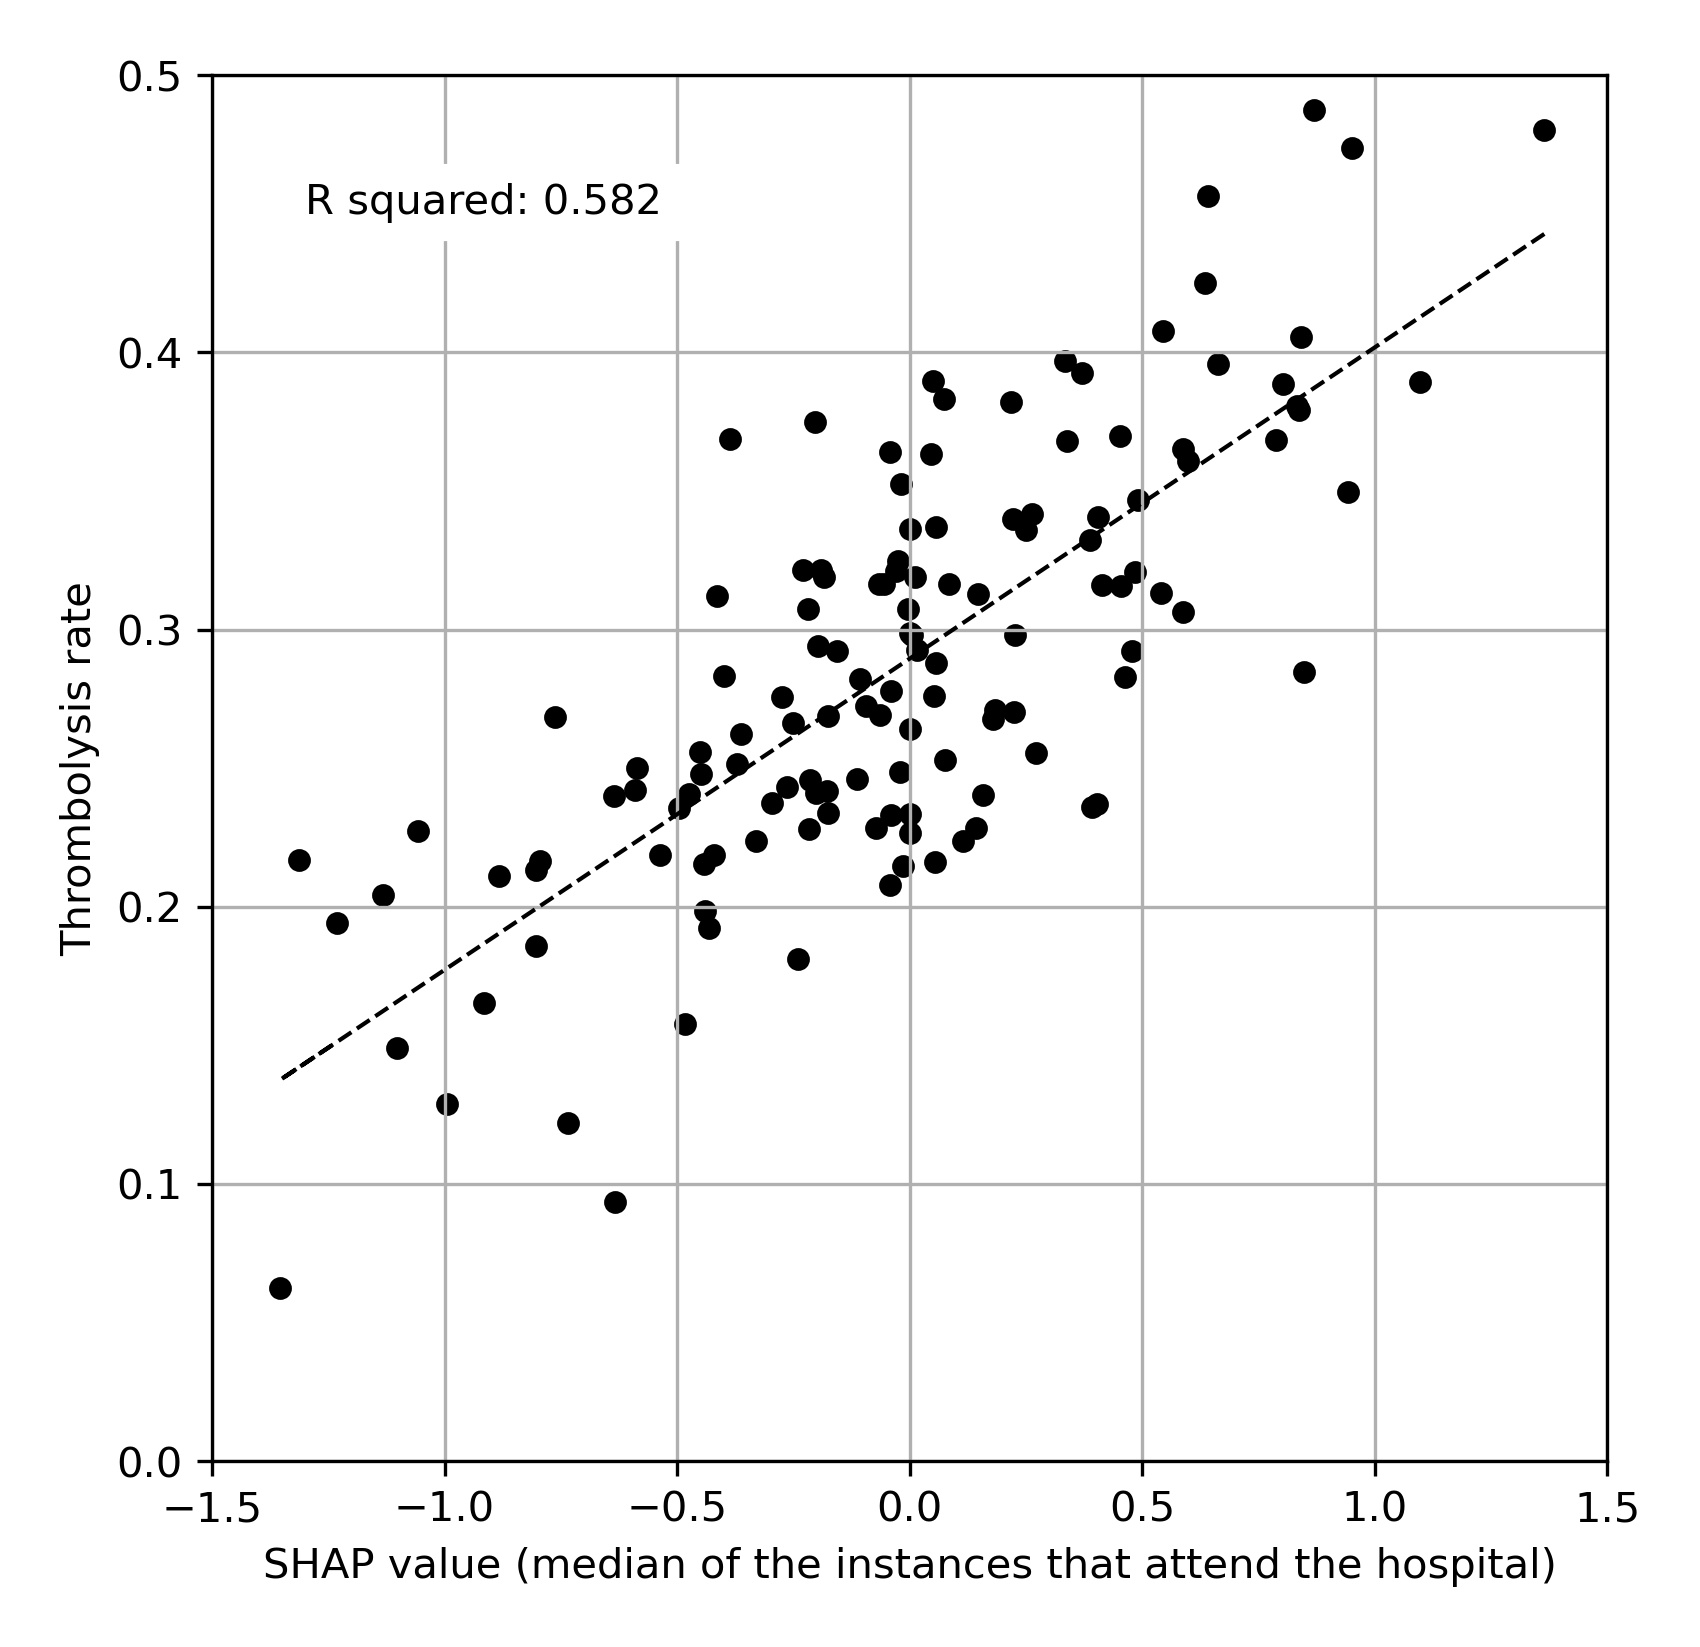
\includegraphics[width=0.7\textwidth]{./images/03c_xgb_10_features_attended_hosp_shap_value}
\caption{Correlation between median hospital SHAP value and the observed thrombolysis use at each hospital.}
\label{fig:shap_correlation_1}
\end{figure}

The hospital SHAP value is composed of a \emph{main} effect of the hospital, independent of other patient features, and \emph{interaction effects}, which is how the hospital ID interacts with other patient features (e.g. if a hospital treats a certain type of patient in a way that is different to the usual pattern). We found that the SHAP value (which is the sum of the \emph{main effect} and the \emph{interaction effects}) for hospitals had a broader range than the main effect (\ref{fig:shap_boxplot_1}), as this value included how a hospital may have different predispositions to use thrombolysis in different types of patient. 

\begin{figure}
\centering
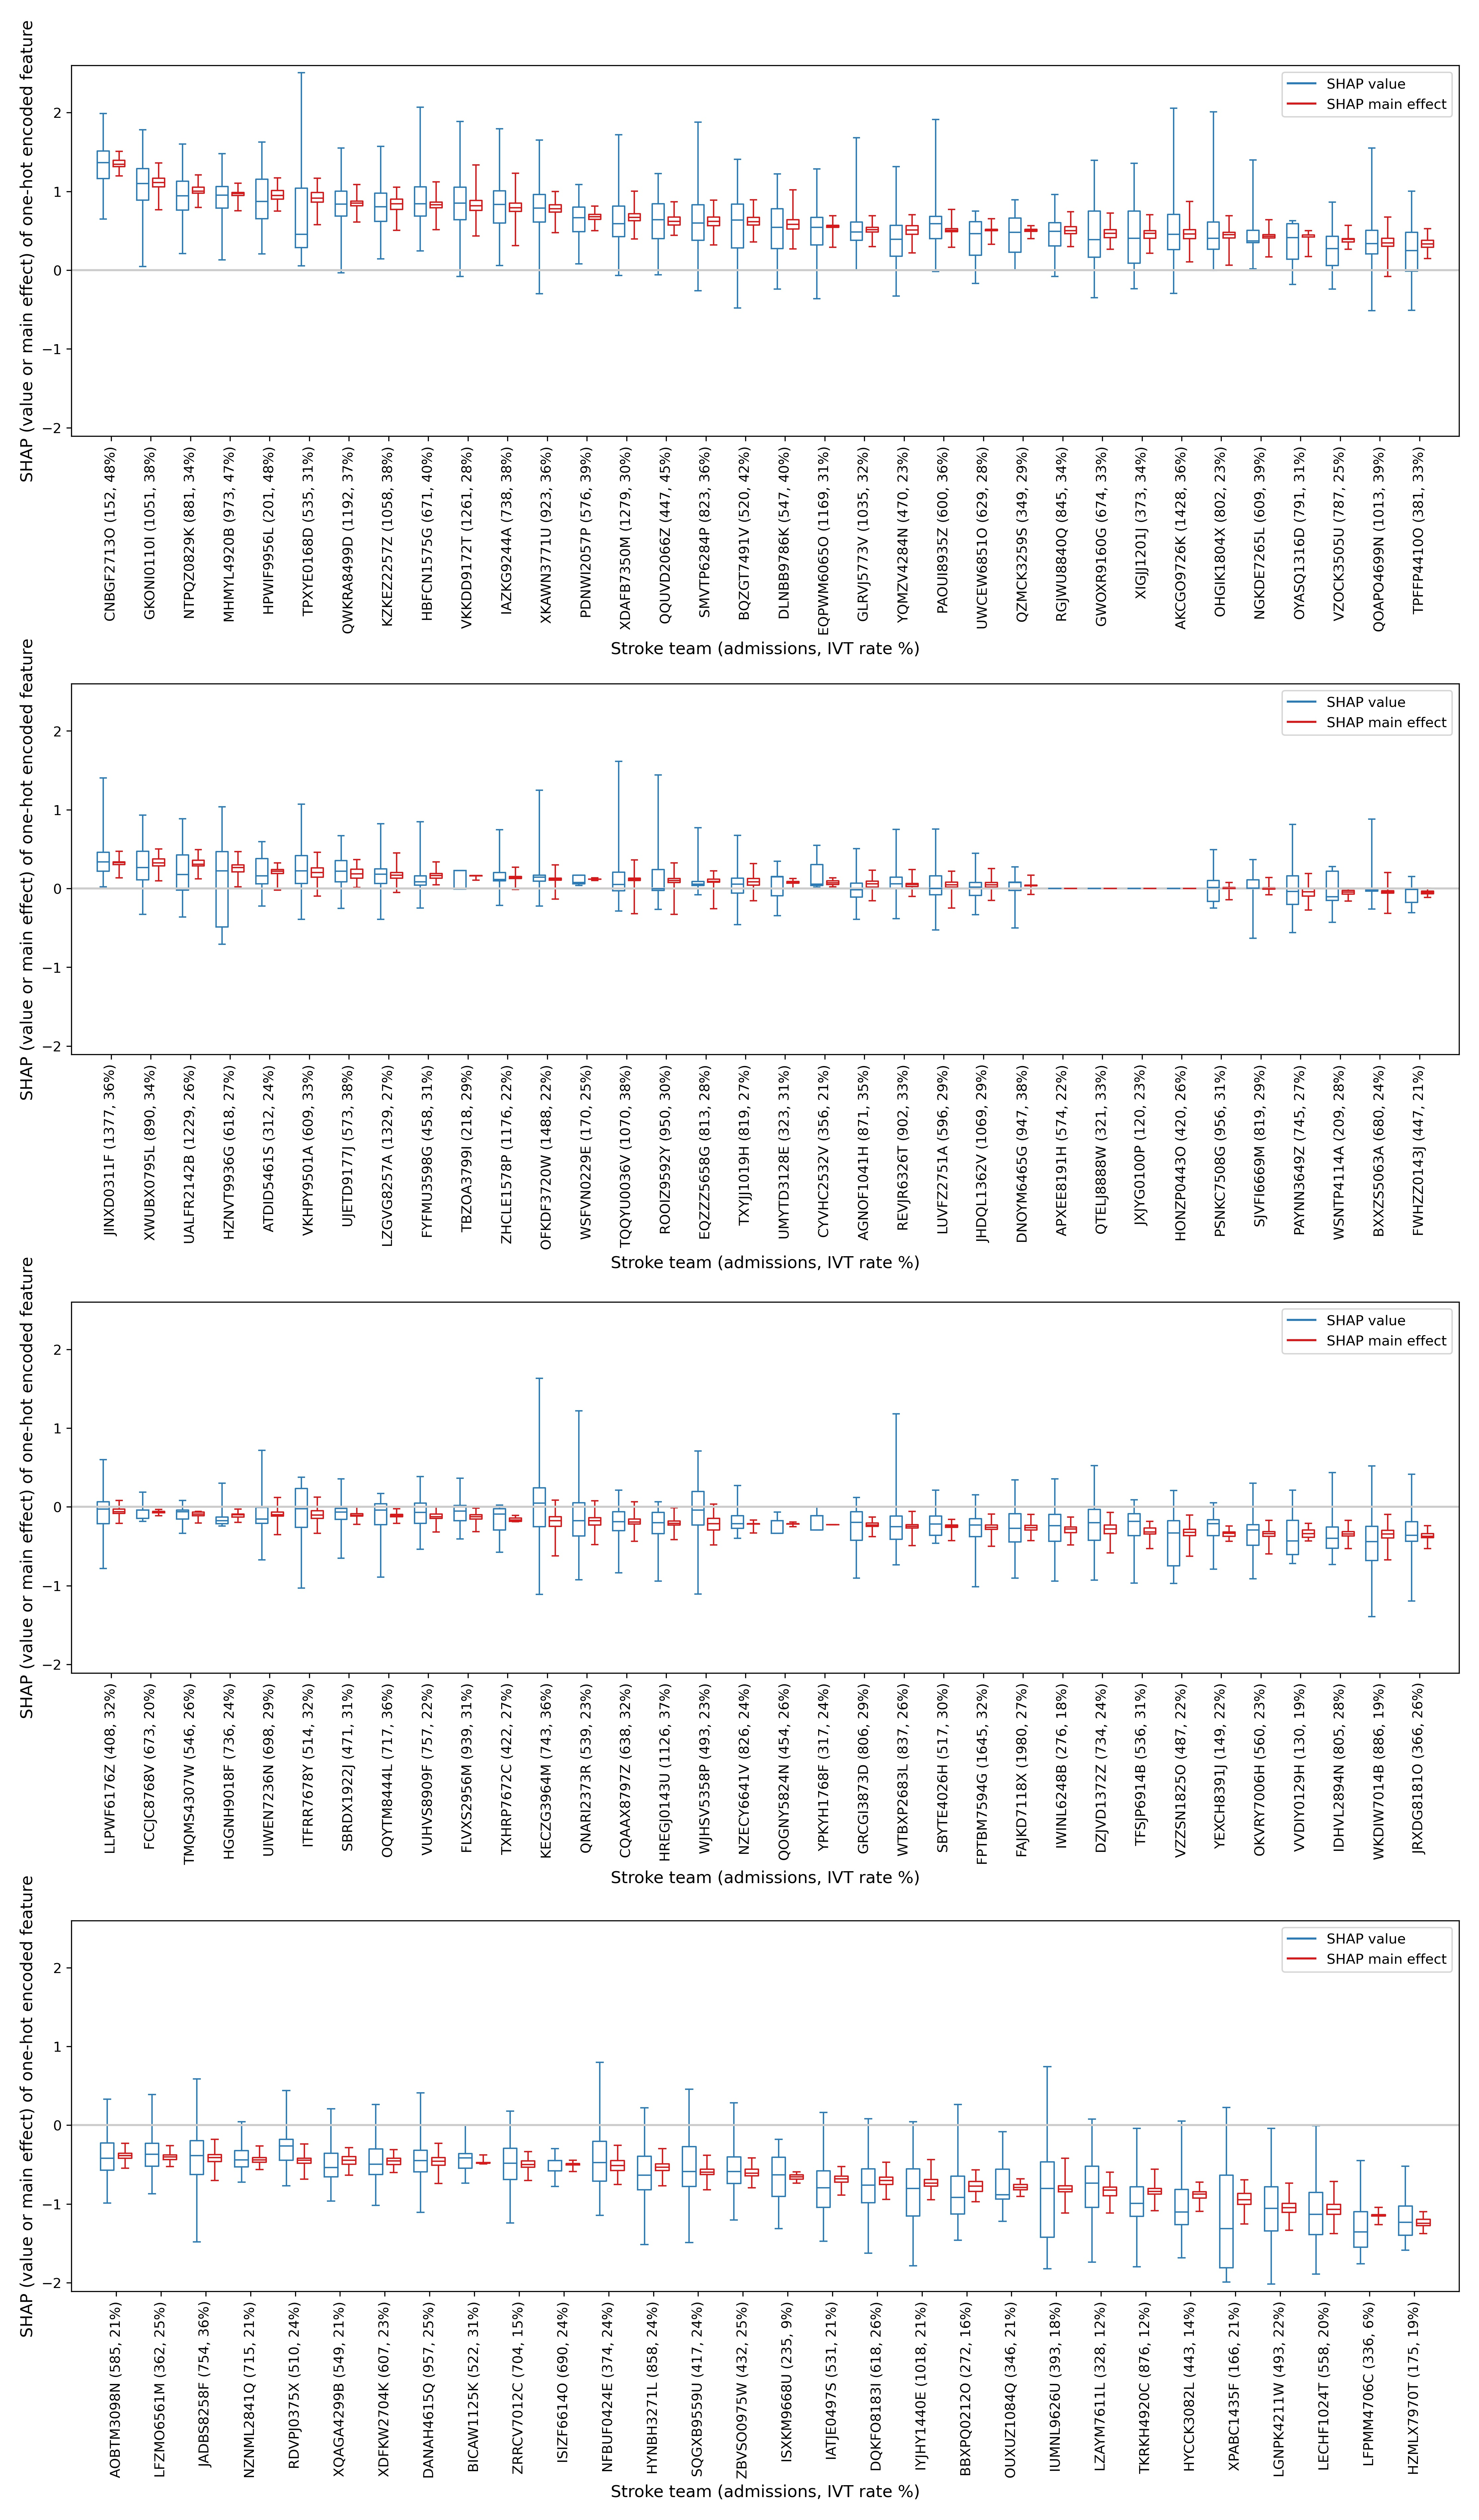
\includegraphics[width=0.85\textwidth]{./images/03c_xgb_10_features_individual_hosp_shap_value_and_main_effect_attend_vs_notattend_boxplot}
\caption{Boxplots for the SHAP value (composed of the sum of the main effect and the interaction effects) and the SHAP main effect value, for each of 132 hospitals.}
\label{fig:shap_boxplot_1}
\end{figure}

When we re-examine the correlation between hospital SHAP and observed thrombolysis rate (figure \ref{fig:shap_correlation_2}, we find that the main hospital SHAP effect accounts for 56\% of the variance in thrombolysis rate (*c.f.* 58\% for the full SHAP).

\begin{figure}
\centering
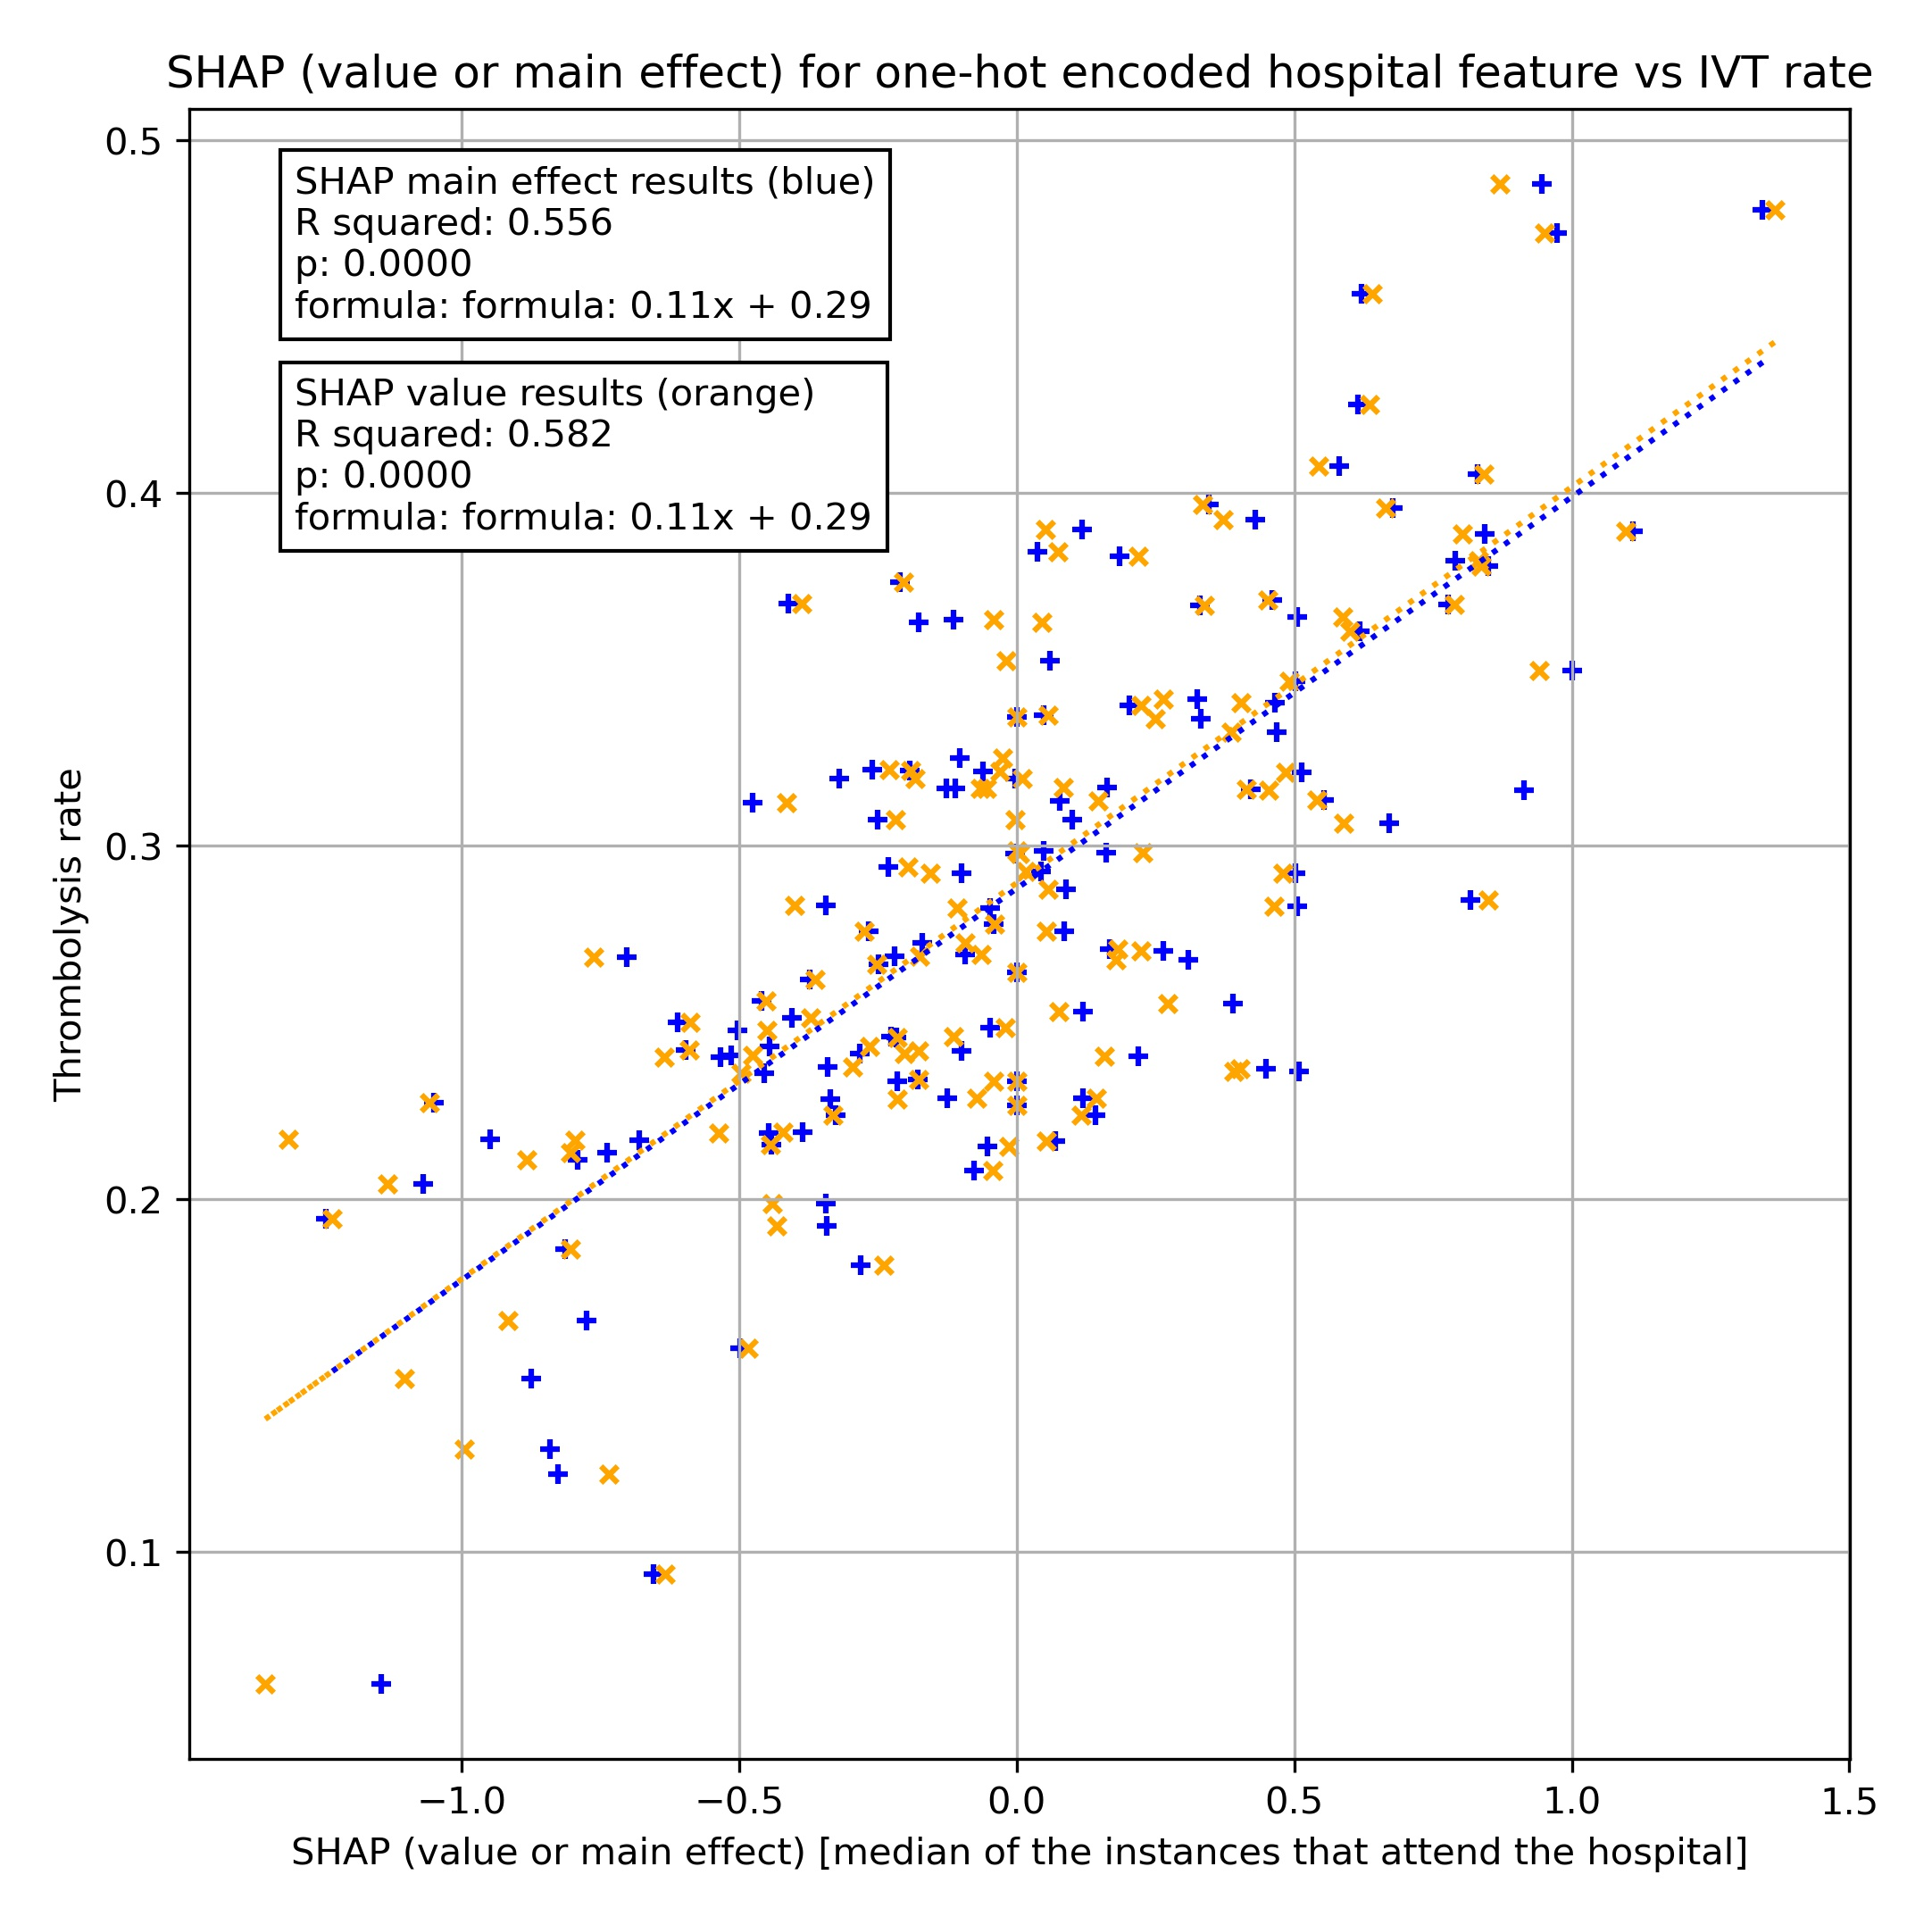
\includegraphics[width=0.85\textwidth]{./images/03c_xgb_10_features_attended_hosp_shap_value_and_main_effect_vs_ivt_rate}
\caption{Correlations between median hospital SHAP value or the median SHAP main effect value, and the observed thrombolysis use at each hospital.}
\label{fig:shap_correlation_2}
\end{figure}

%%%%%%%%%%%%%%%%%%%%%%%%%%%%%%%%%%%%%%%%%%%%%%%%%%%%%%%%%%%%%%%%%%%%%%%%%%%%%%%%%%%%%%%

\subsubsection{Hospital SHAP and 10k cohort}

When using the 10k cohort, changing the one-hot encoding to mimic all patients attending each of the 132 hospitals, we found that the median hospital SHAP value for the 10k patients correlated very closely with the predicted thrombolysis use in the 10k cohort at each hospital (figure \ref{fig:shap_correlation_3}, r-squared = 0.947 for full SHAP and r-squared = 0.944 for the main effect), confirming that the hospital SHAP is providing a key insight into a hospital's predisposition to use thrombolysis.

\begin{figure}
\centering
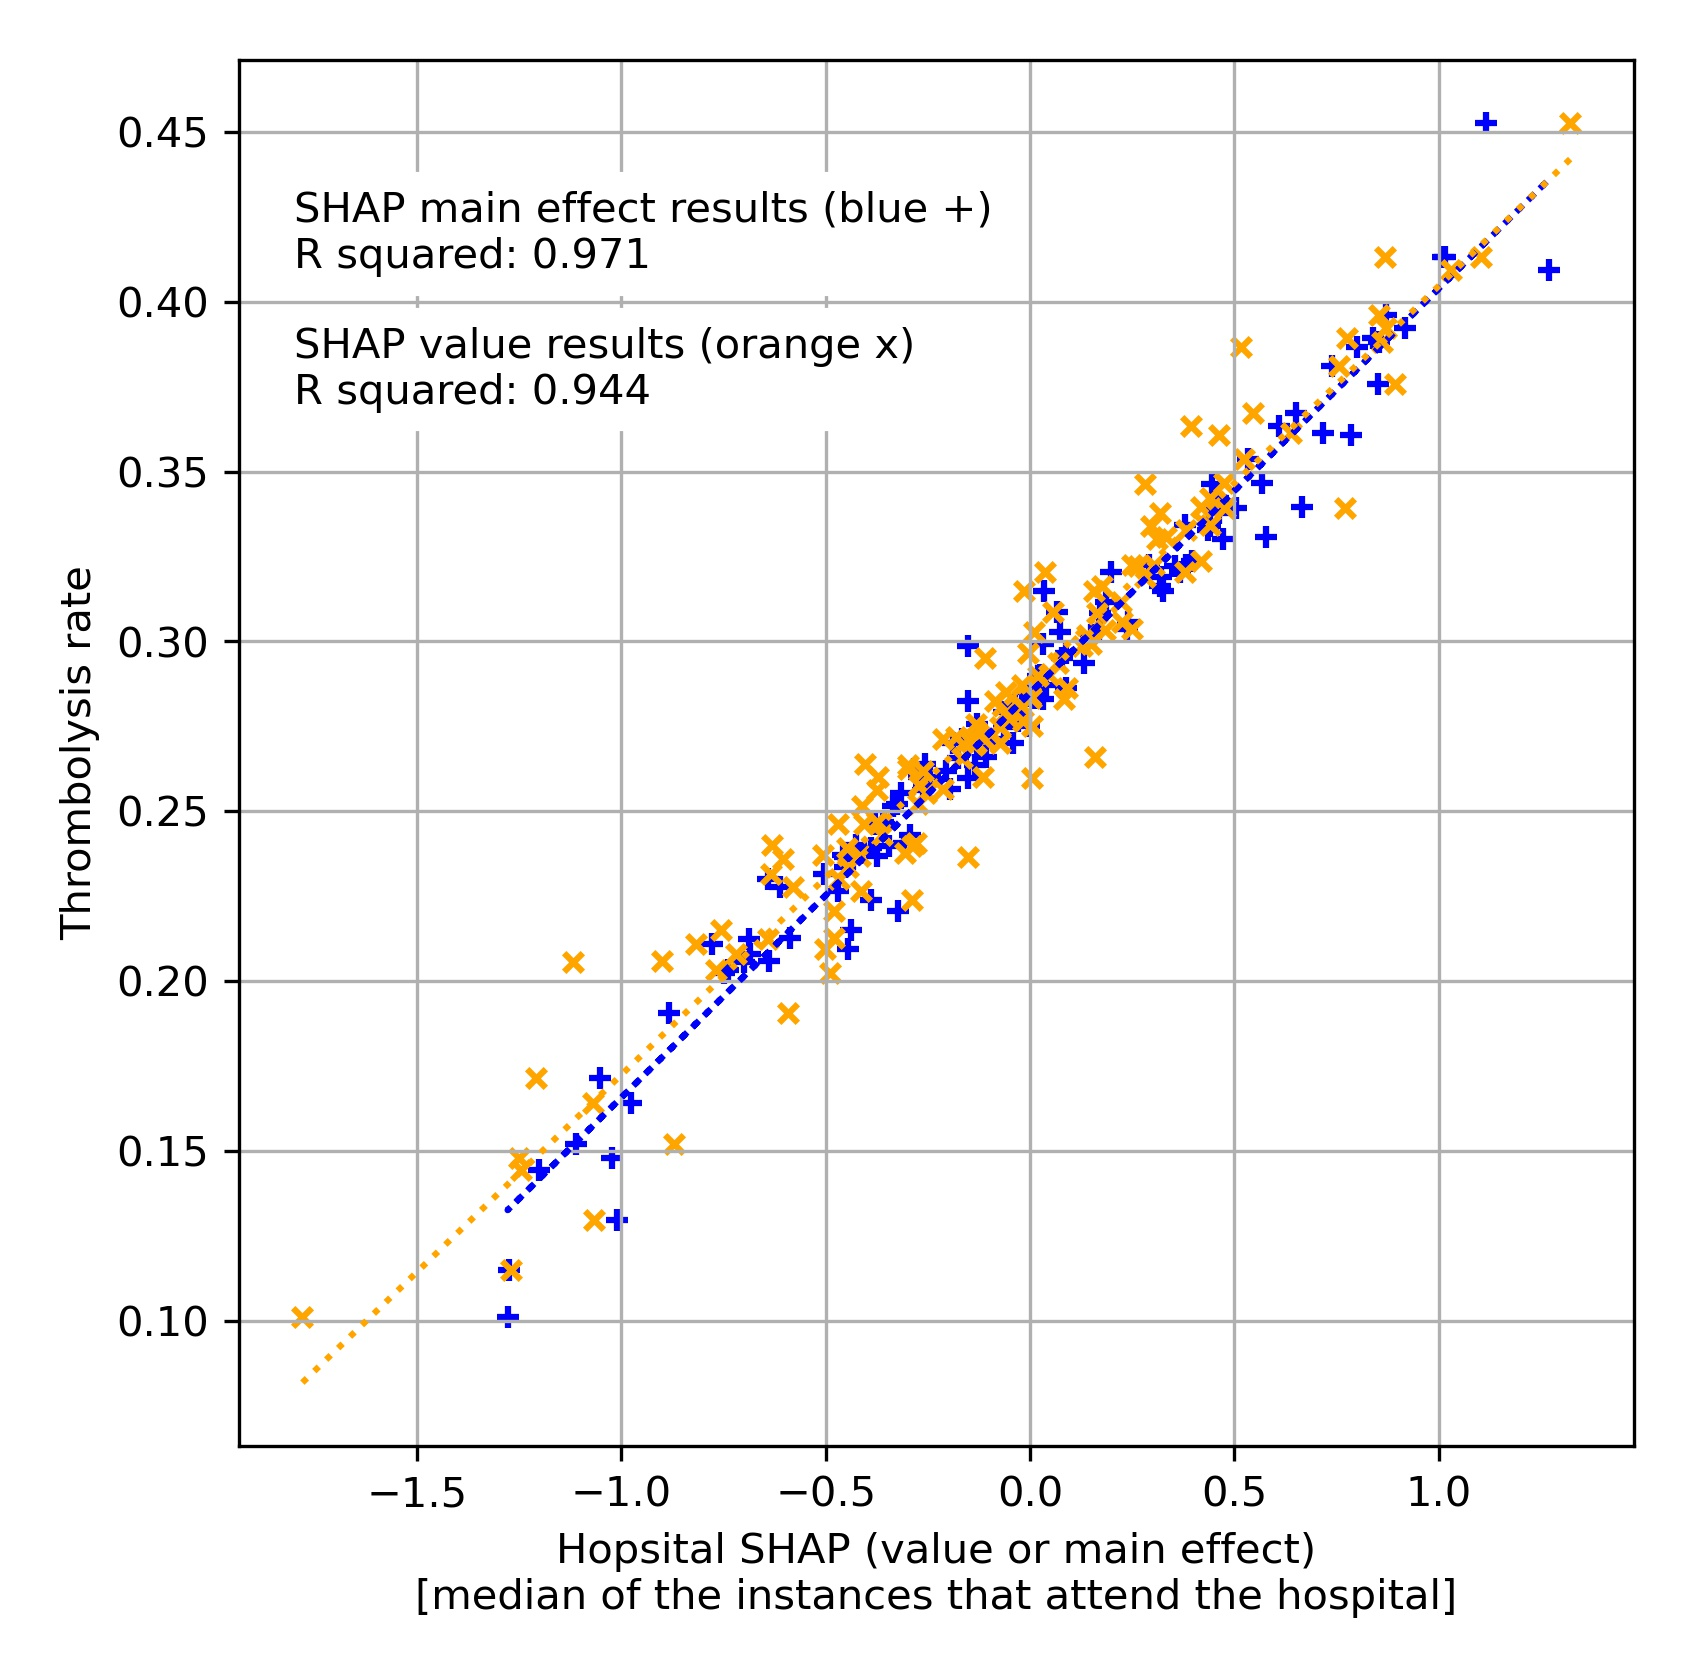
\includegraphics[width=0.85\textwidth]{./images/04_xgb_10_features_10k_cohort_attended_hosp_shap}
\caption{Correlations between median hospital SHAP value or the median SHAP main effect value, and the predicted thrombolysis rate of the 10k cohort of patients at each hospital.}
\label{fig:shap_correlation_3}
\end{figure}

Though we model the same 10k patients going to all hospitals, we found that the SHAP interaction effect (the difference between the full SHAP value and the SHAP main effect) differed between hospitals (figure \ref{fig:shap_boxplot_2}). This demonstrated how the hospital SHAP is partly dependent on the patients attending (and the hospital's predisposition to give thrombolysis to different groups of patients).

\begin{figure}
\centering
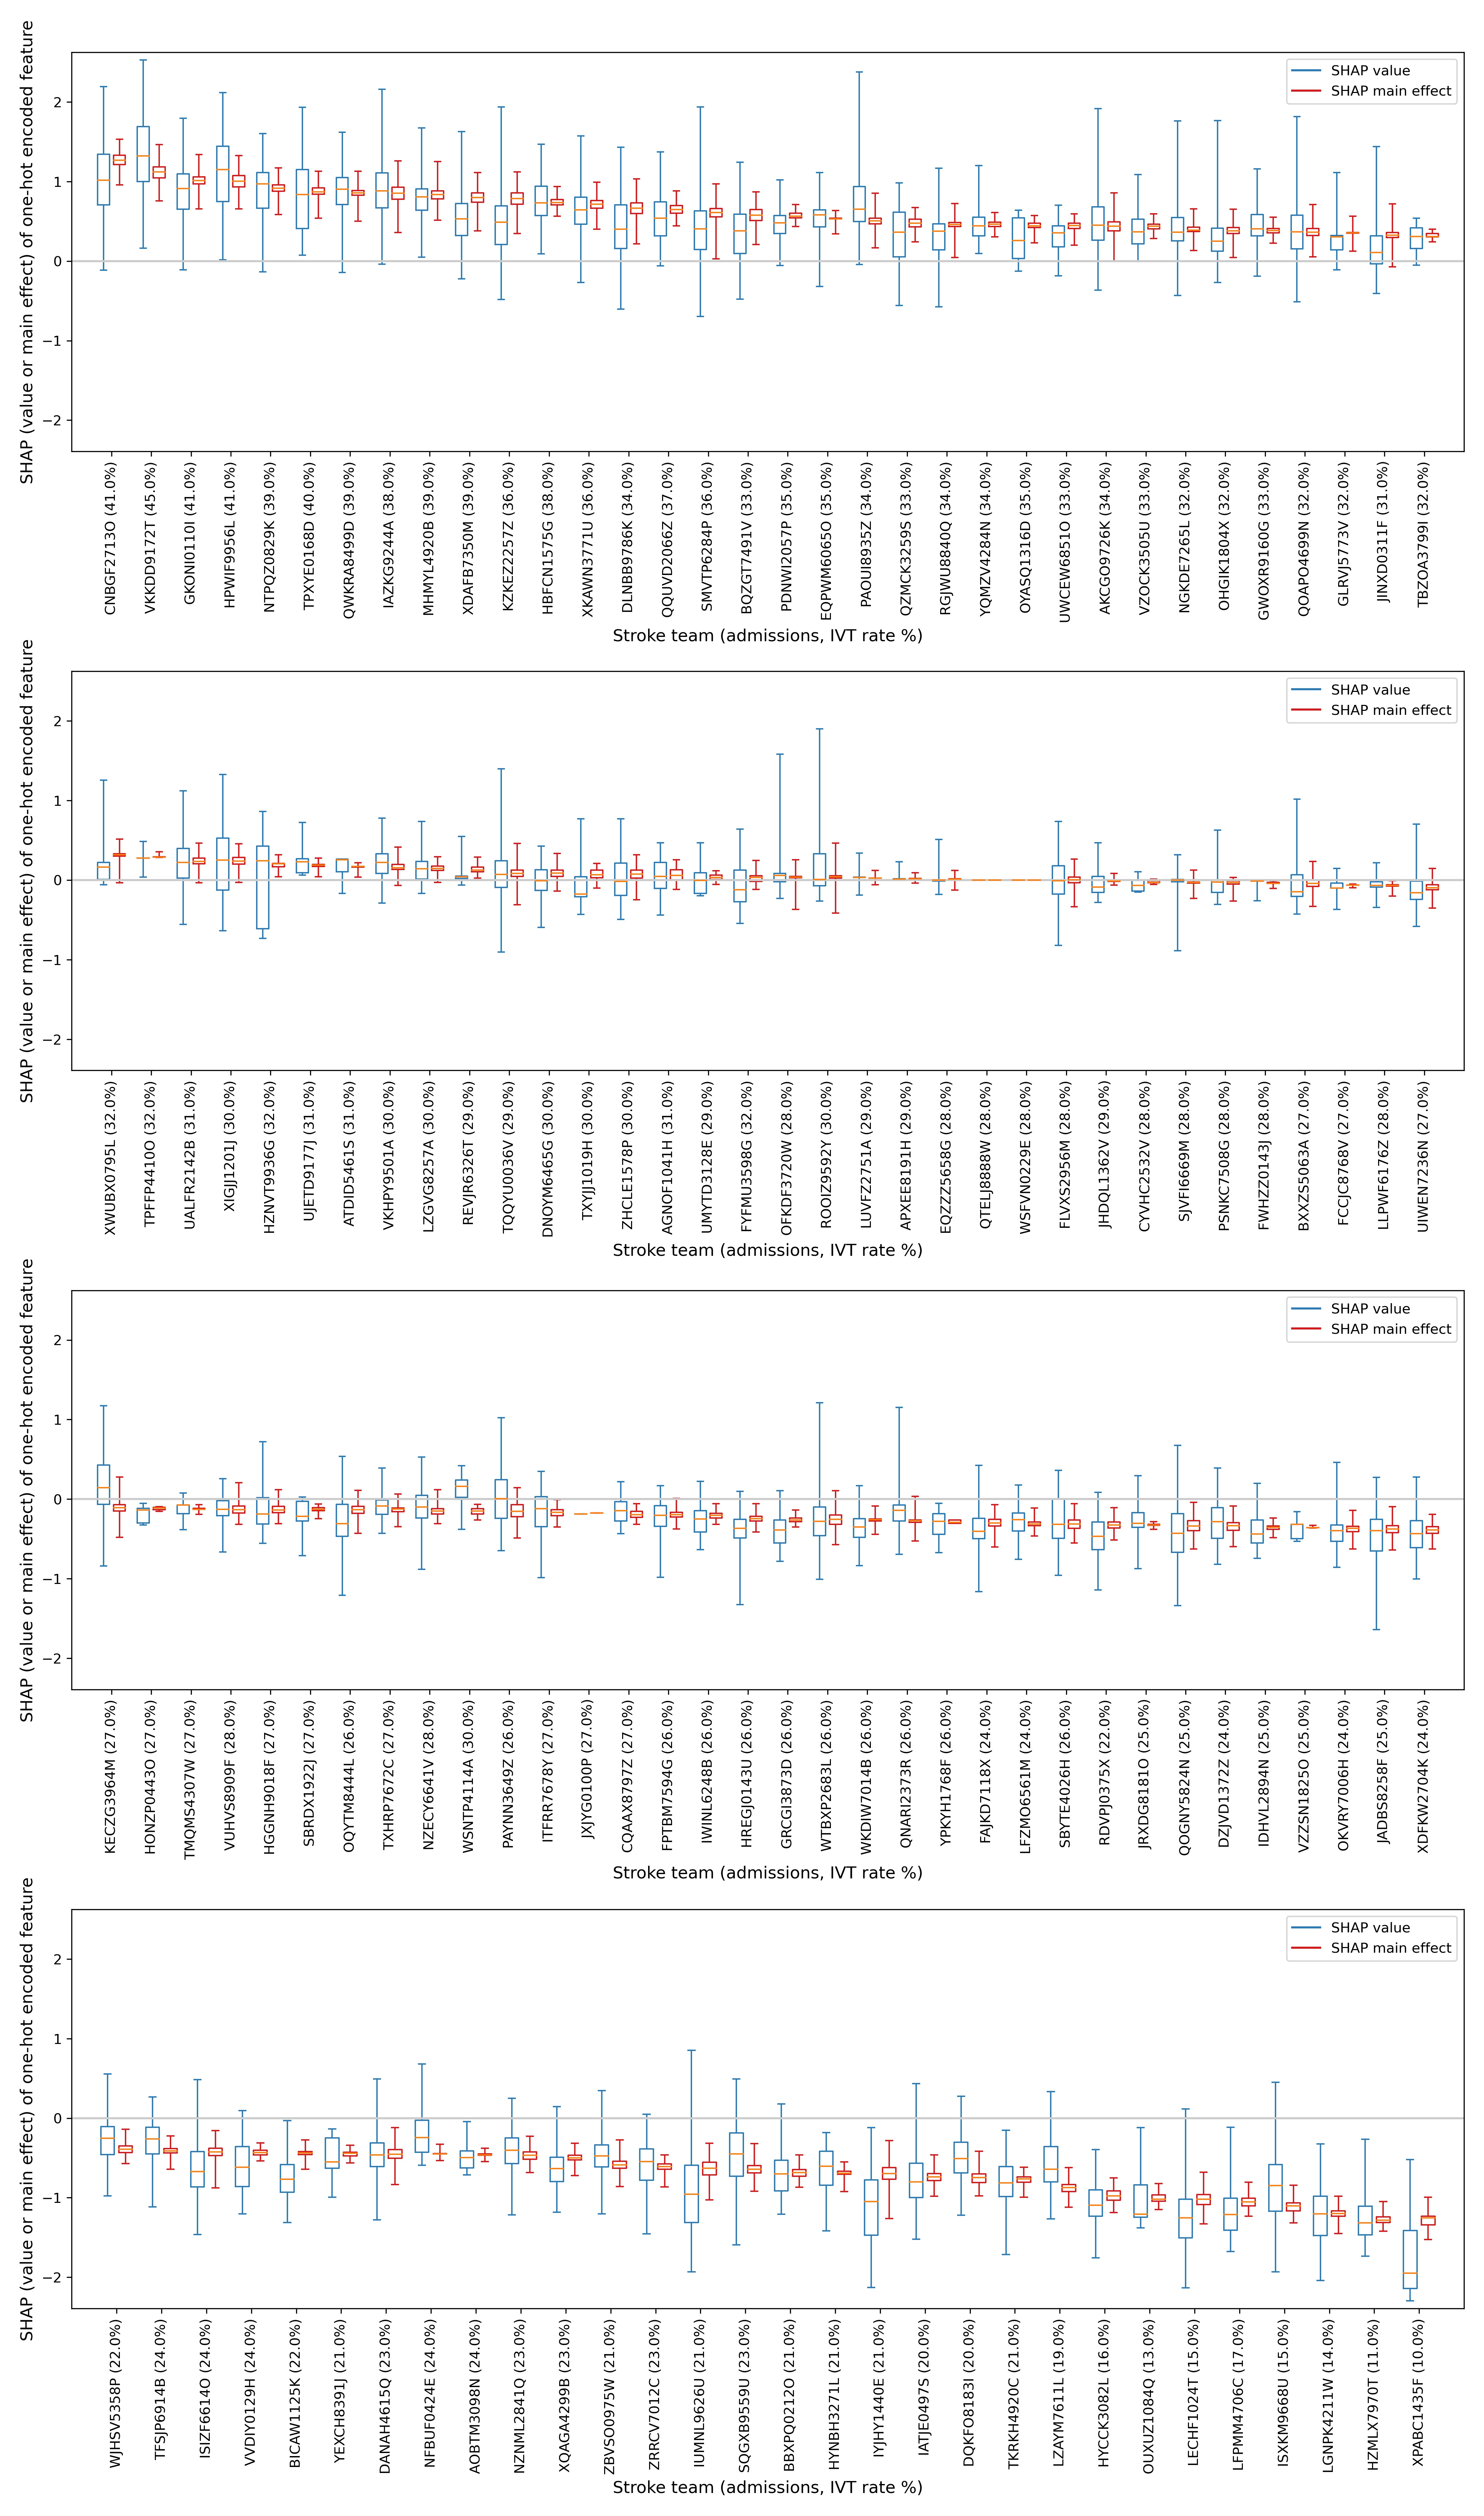
\includegraphics[width=0.85\textwidth]{./images/04_xgb_10_features_10k_cohort_individual_hosp_shap_value_and_maineffect_attend_vs_notattend_boxplot}
\caption{Boxplots for the SHAP value (composed of the sum of the main effect and the interaction effects) and the SHAP main effect value, for each of 132 hospitals, when evaluated with the 10k patient cohort.}
\label{fig:shap_boxplot_2}
\end{figure}


%%%%%%%%%%%%%%%%%%%%%%%%%%%%%%%%%%%%%%%%%%%%%%%%%%%%%%%%%%%%%%%%%%%%%%%%%%%%%%%%%%%%%%%

\subsection{Hospital SHAP interactions}

Below are three examples of how a particular hospital modified the general SHAP effects - either strengthening the effect, of attenuating it.

%%%%%%%%%%%%%%%%%%%%%%%%%%%%%%%%%%%%%%%%%%%%%%%%%%%%%%%%%%%%%%%%%%%%%%%%%%%%%%%%%%%%%%%

\subsubsection{Hospital and onset time interaction}

The main effect of the *precise onset time* is that if onset time is known precisely then SHAP (log odds) is increased by 0.42, otherwise it is reduced by 0.85.

Team HZNVT9936G has a slightly higher main effect for hospital SHAP (0.26) than team FAJKD7118X (-0.27). As is seen in figure \ref{fig:interaction_precise}, team HZNVT9936G has interactions that strengthen the effect of \emph{precise onset time} whereas team FAJKD7118X has interactions values that attenuate the main effect of \emph{precise onset time}.

\begin{figure}
\centering
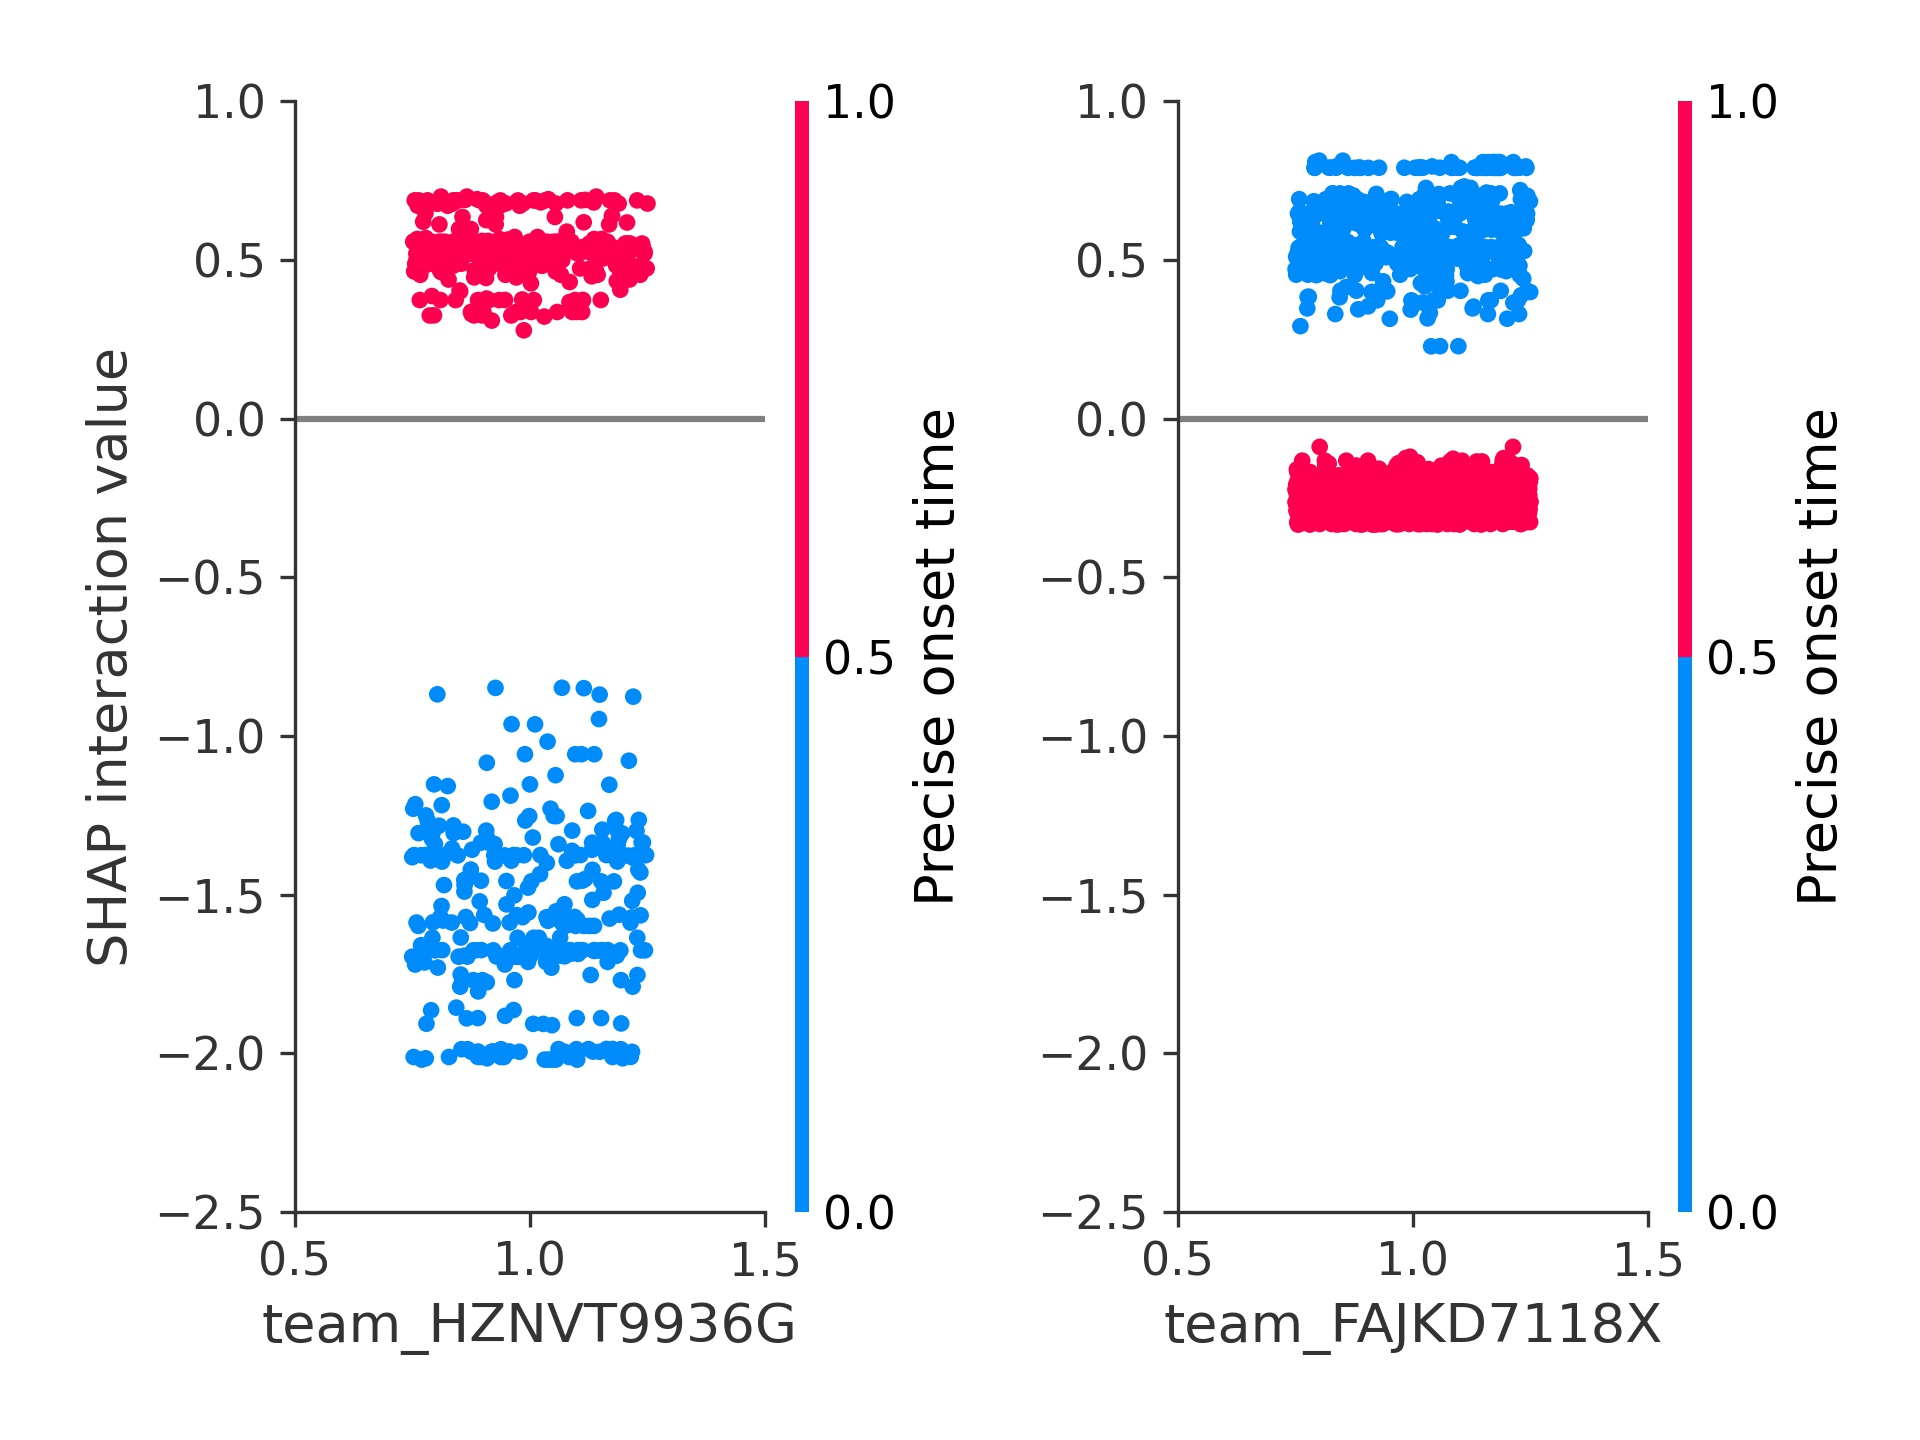
\includegraphics[width=0.7\textwidth]{./images/12aa_onset_time_type_interaction_example}
\caption{SHAP interaction between hospital ID for two teams and whether stroke onset time was known precisely. If a patient attended team HZNVT9936G then SHAP value for having a precise onset time was increased (a strengthening of the main effect of precise onset time). If a patient attended team FAJKD7118X then SHAP value for having a precise onset time was reduced (an attenuation of the main effect of precise onset time).}
\label{fig:interaction_precise}
\end{figure}

%%%%%%%%%%%%%%%%%%%%%%%%%%%%%%%%%%%%%%%%%%%%%%%%%%%%%%%%%%%%%%%%%%%%%%%%%%%%%%%%%%%%%%%

\subsubsection{Hospital and stroke severity interaction}

The main effect of stroke severity is to significantly reduce the odds of receiving thrombolysis for mild strokes (NIHSS 0-5), increase the odds of receiving thrombolysis for more moderate to sever strokes (NIHSS 6-32), and then reduce the odds of receiving thrombolysis for very severe stroke strokes (NIHSS 33+).

Team TPXYE0168D has a higher general tendency to use thrombolysis than team SMVTP6284P (team main effect SHAP = 0.92 vs 0.62). As is seen in figure \ref{fig:interaction_nihss}, team TPXYE0168D has a SHAP interaction that opposes the general stroke severity main effect, especially attenuating the reduced odds of receiving thrombolysis for mild strokes from the main effect of stroke severity. Team SMVTP6284P strengthens the main effect of stroke severity - reducing the odds of receiving thrombolysis even further for mild strokes.

\begin{figure}
\centering
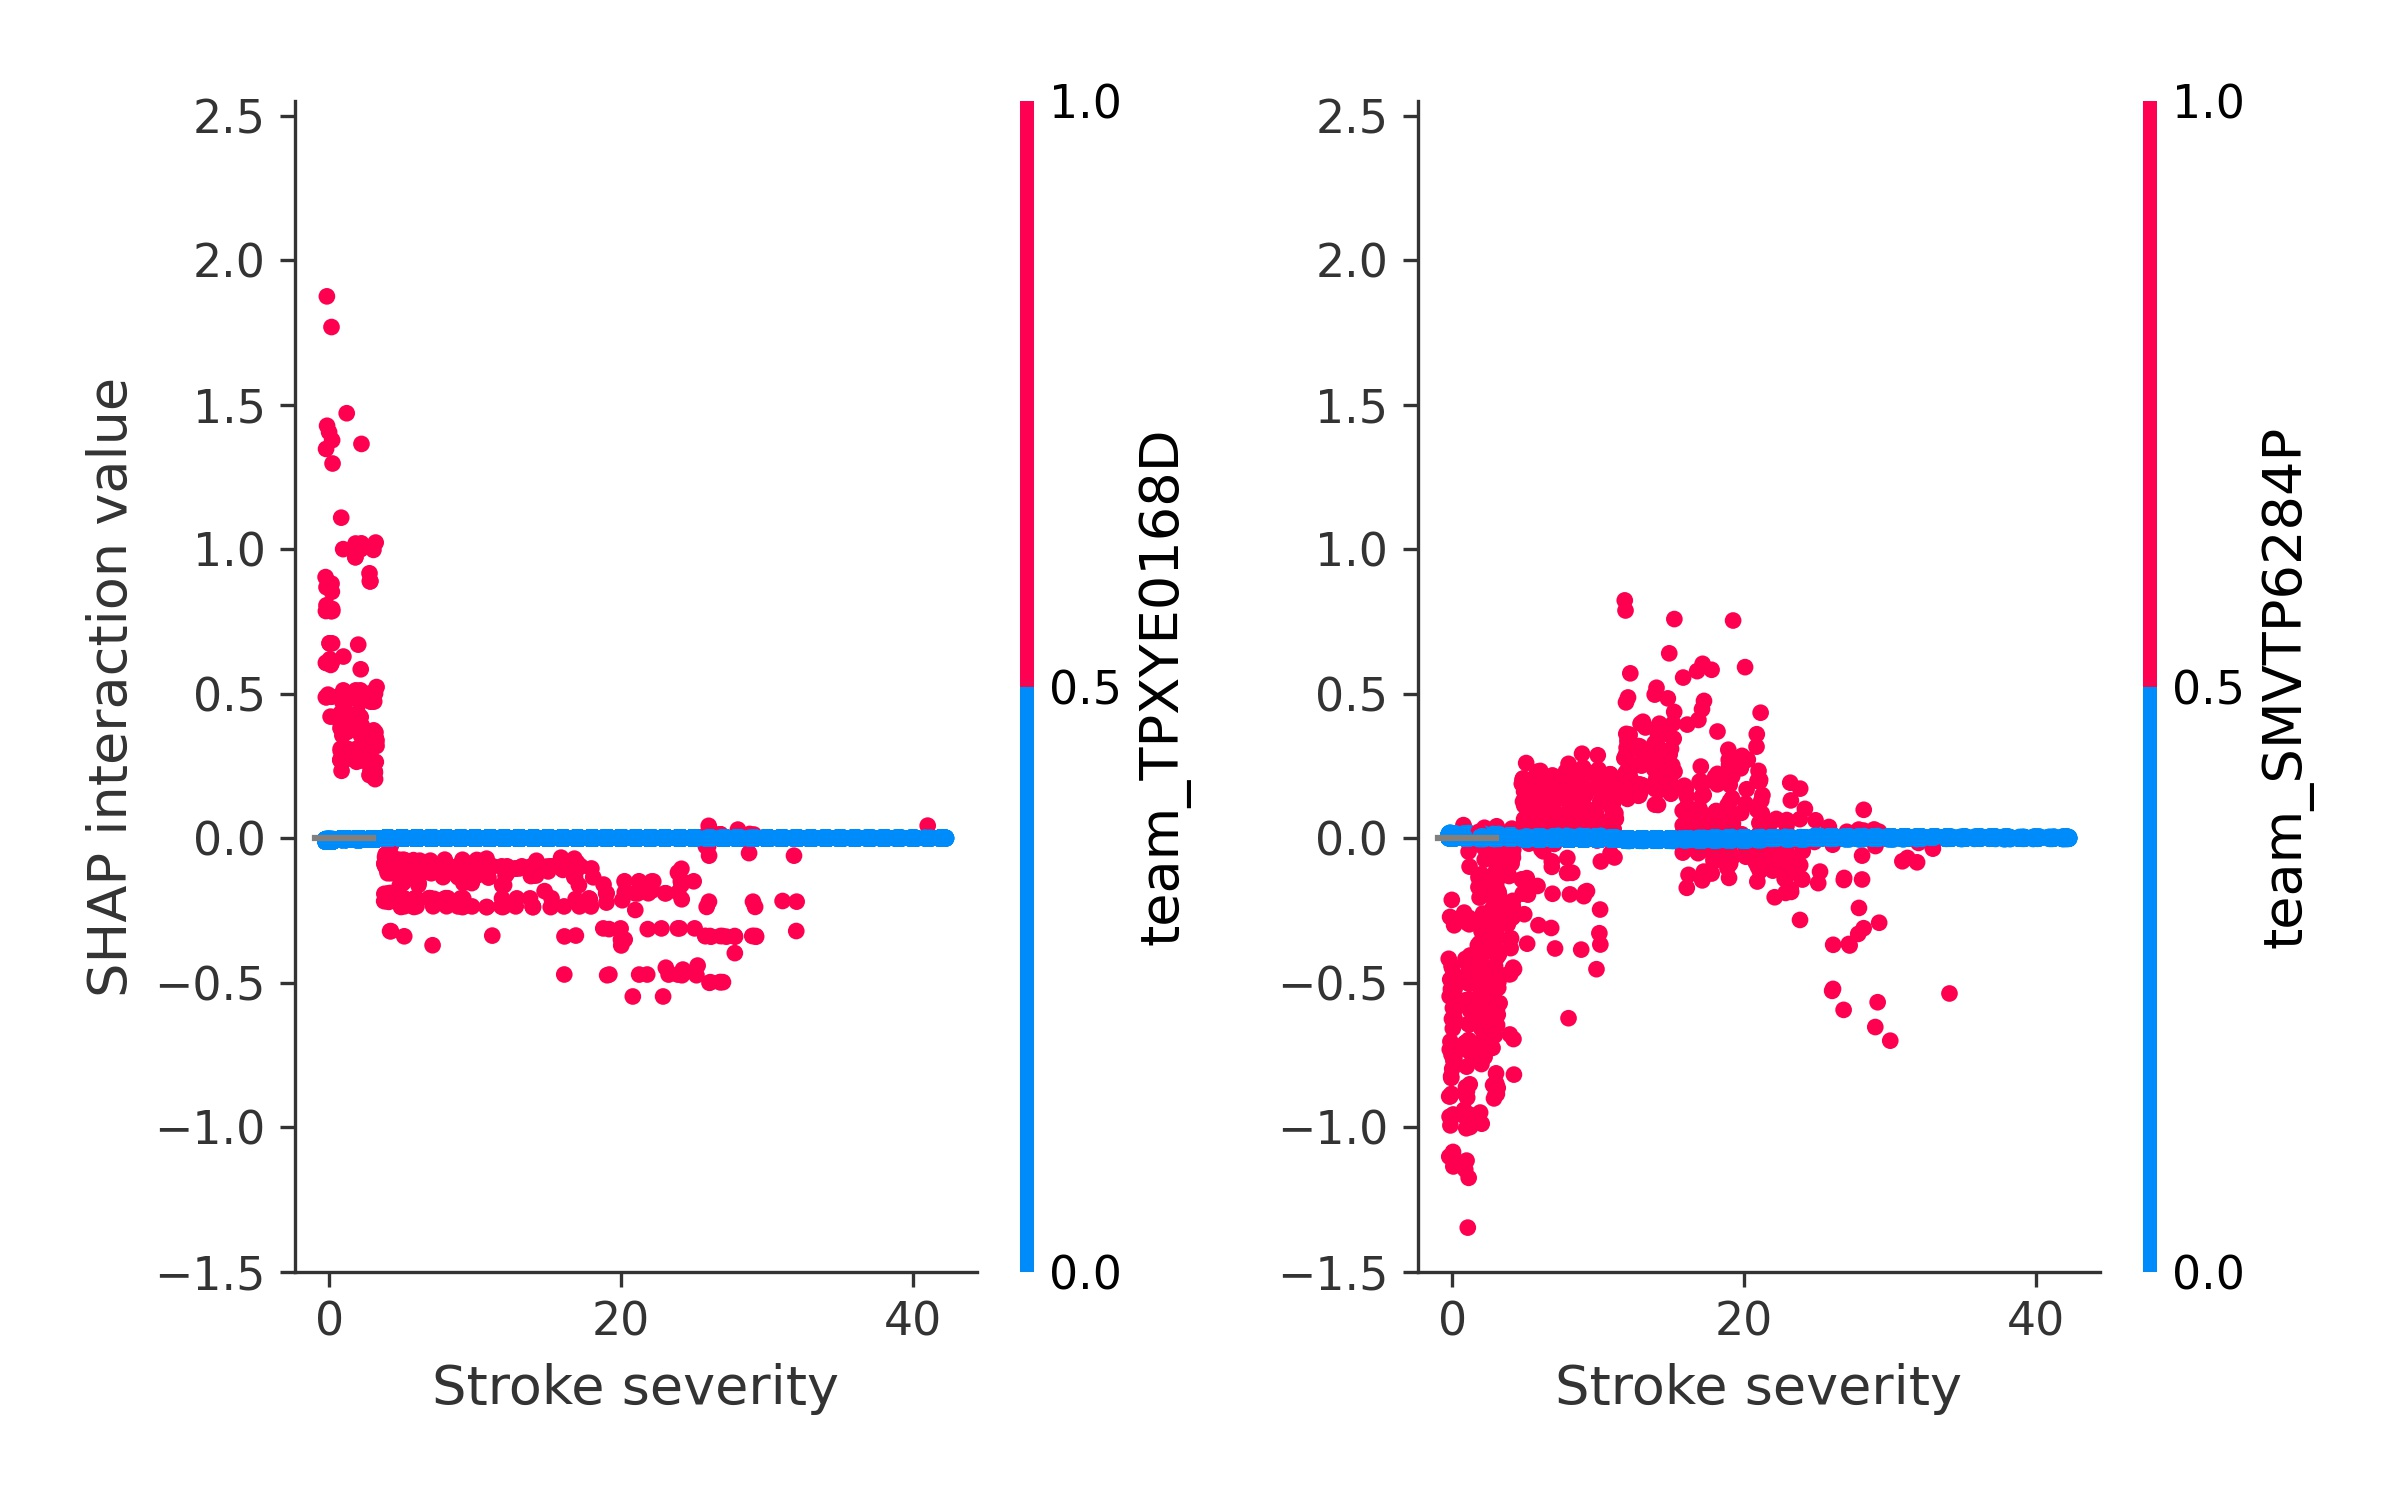
\includegraphics[width=0.7\textwidth]{./images/12ab_stroke_severity_interaction_example}
\caption{SHAP interaction between hospital ID for two teams and stroke severity. If a patient attended team TPXYE0168D then SHAP values for low stroke severity were increased (an attenuation of the main effect of stroke severity). If a patient attended team SMVTP6284P then SHAP values for low and severe stroke severity were reduced (a strengthening of the main effect of stroke severity).}
\label{fig:interaction_nihss}
\end{figure}

%%%%%%%%%%%%%%%%%%%%%%%%%%%%%%%%%%%%%%%%%%%%%%%%%%%%%%%%%%%%%%%%%%%%%%%%%%%%%%%%%%%%%%%

\subsubsection{Hospital and and prior disability interaction}

The main effect of prior disability is to progressively reduce the odds of receiving thrombolysis with increasing disability (a SHAP of +0.3 for mrS=0 down to -1.50 for mRS=5). As is seen in figure \ref{fig:interaction_mrs}, team XKAWN3771U has a slightly higher general tendency to use thrombolysis than team AKCGO9726K (team main effect SHAP = 0.78 vs 0.45). Team XKAWN3771U has a SHAP interaction that attenuates the general prior disability main effect. Team AKCGO9726K strengthens the main effect of pre-stroke disability,reducing the odds of receiving thrombolysis even further for mild strokes.

\begin{figure}
\centering
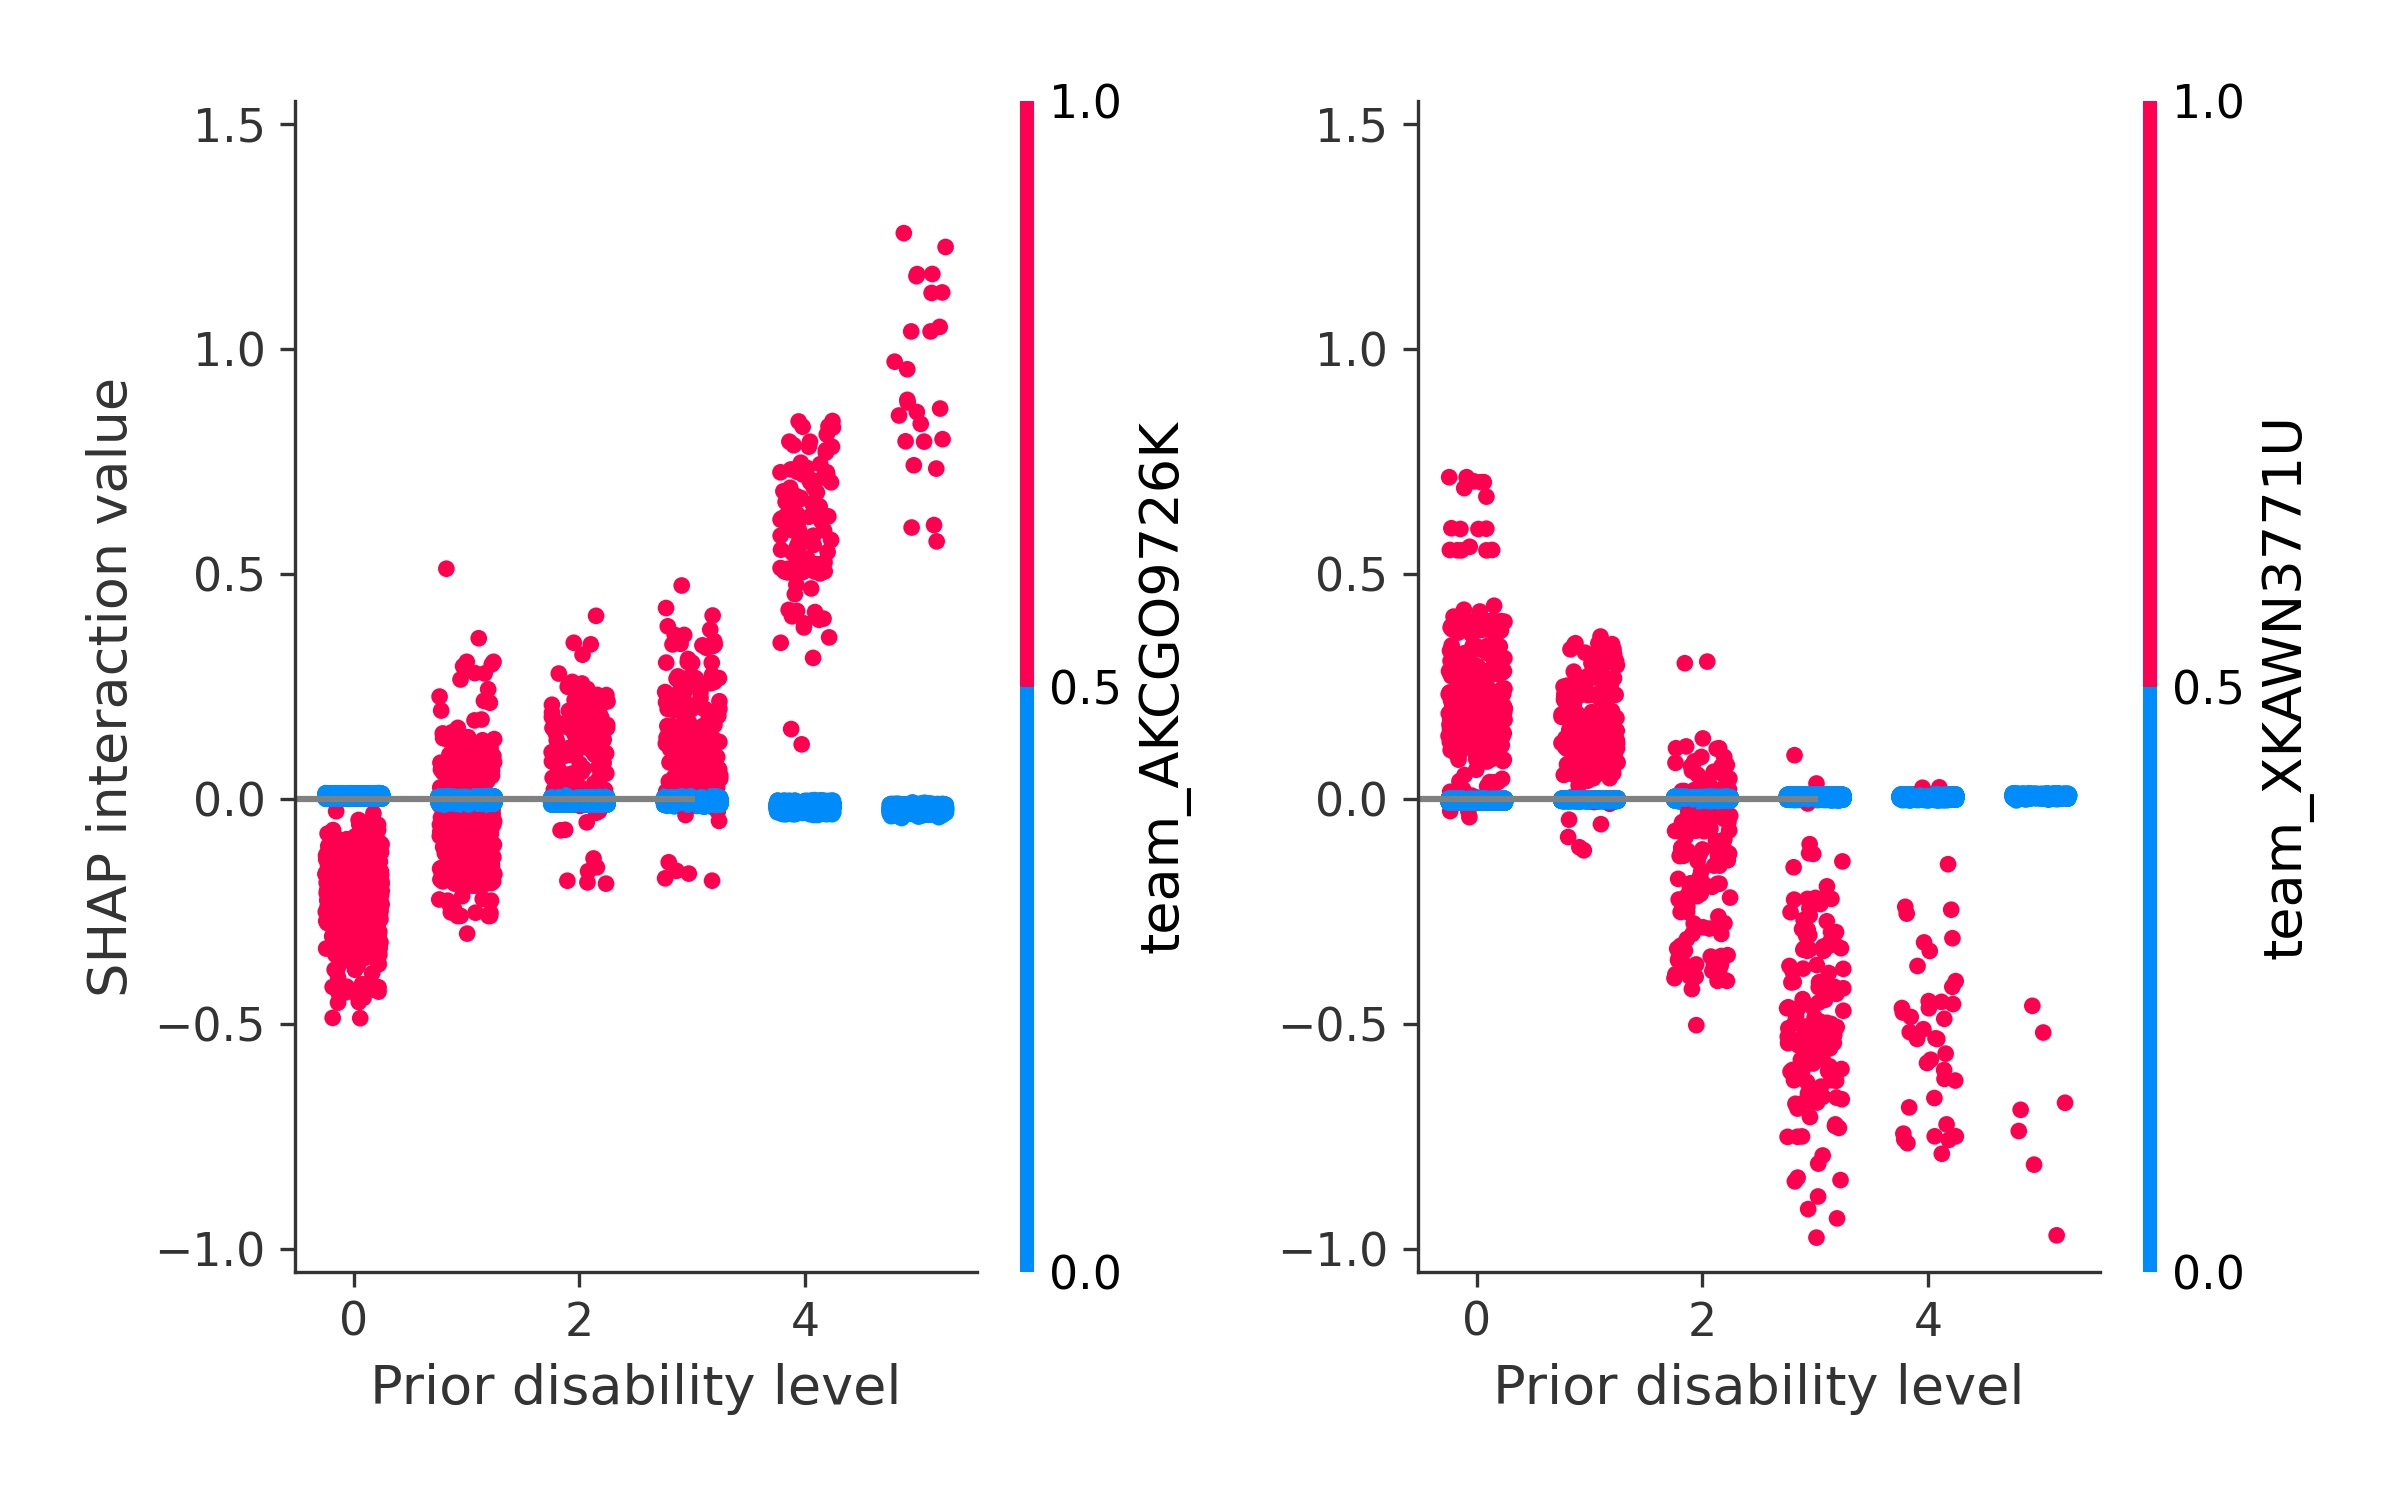
\includegraphics[width=0.7\textwidth]{./images/12ac_disability_interaction_example}
\caption{SHAP interaction between hospital ID for two teams and pre-exisiting disability. If a patient attended team AKCGO9726K then SHAP values for increasing pre-stroke disability were increased (an attenuation of the main effect of stroke severity). If a patient attended team XKAWN3771U then SHAP values for increasing pre-stroke disability were reduced (a strengthening of the main effect of stroke severity).}
\label{fig:interaction_mrs}
\end{figure}

%%%%%%%%%%%%%%%%%%%%%%%%%%%%%%%%%%%%%%%%%%%%%%%%%%%%%%%%%%%%%%%%%%%%%%%%%%%%%%%%%%%%%%%

\subsection{General SHAP interactions}

All features may interact with each other, and SHAP captures all these 2-way interactions. We found that the feature main effects (without interactions) accounted for 62\% of the total SHAP values, and 38\% of the total SHAP values came from interactions. Figure \ref{fig:shap_interactions} shows interactions between all features, excluding the one-hot encoded hospitals.

\begin{figure}
\centering
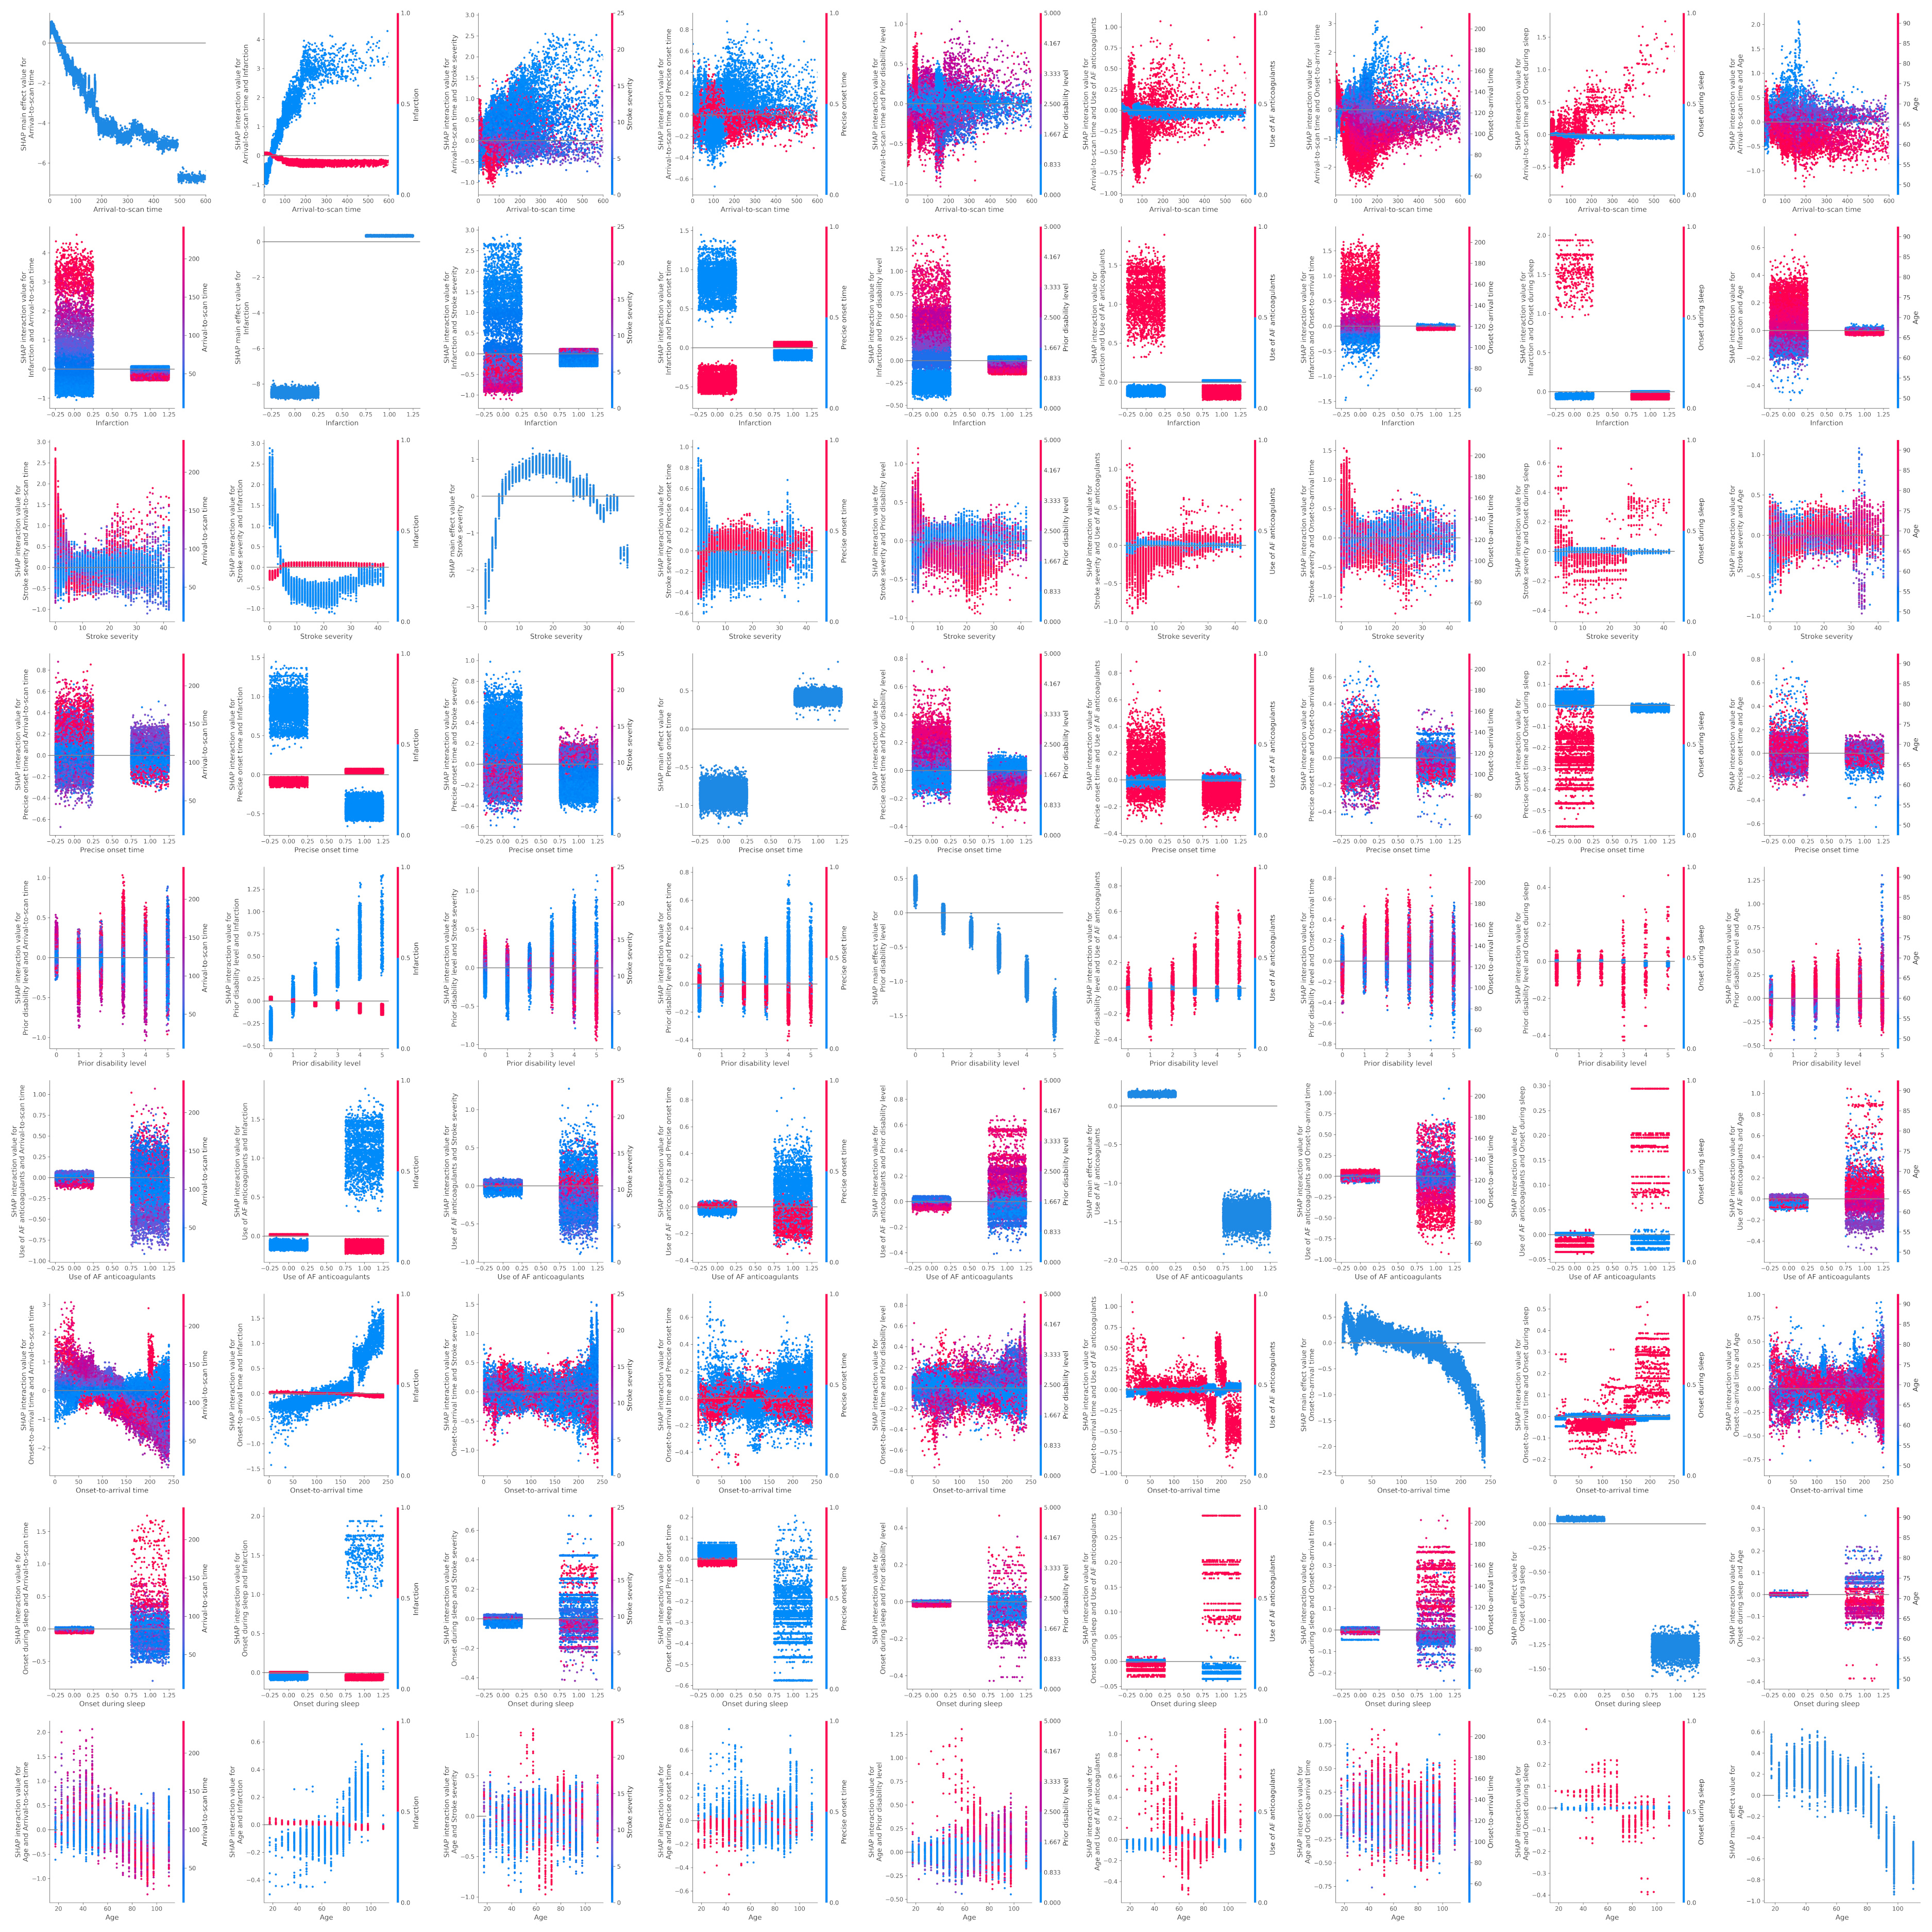
\includegraphics[width=1.0\textwidth]{./images/12a_shap_interactions_scatter_small}
\caption{SHAP interactions between all features, excluding hospital attended. One feature is shown on the x-axis, and the other feature is colour-coded (from blue for low feature values, and red for high feature values). The y-axis shows the value of the SHAP interaction between the two features; that is the additional value added to the main SHAP effects of each feature.}
\label{fig:shap_interactions}
\end{figure}

Some key interactions identified were:

\begin{itemize}
    \item If a stroke is haemorrhagic, then the interaction is such that the presence of haemorrhage cancels out much of the other SHAP effects (i.e. stroke severity does not matter if the stroke is haemorrhagic).
    \item Likewise elsewhere we find that features that each give negative SHAP values alone have an interaction that attenuates the combined effect of the two features together a little.
\end{itemize}

%%%%%%%%%%%%%%%%%%%%%%%%%%%%%%%%%%%%%%%%%%%%%%%%%%%%%%%%%%%%%%%%%%%%%%%%%%%%%%%%%%%%%%%

\subsection{Subgroup analysis}

We analyse the observed and predicted use of thrombolysis in subgroups of patients.Those groups are:

\begin{itemize}
\item Mild stroke severity (NIHSS \textless{} 5)
\item No precise onset time
\item Existing pre-stroke disability (mRS \textgreater{} 2)
\item An \emph{ideal} thrombolysable patient:
  \begin{itemize}
  \item Stroke severity NIHSS in range 10-25
  \item Arrival-to-scan time \textless{} 30 minutes
  \item Stroke type = infarction
  \item Precise onset time = True
  \item Prior disability level (mRS) = 0
  \item No use of AF anticoagulants
  \item Onset-to-arrival time \textless{} 90 minutes
  \item Age \textless{} 80 years
  \item Onset during sleep = False
  \end{itemize}
\end{itemize}

For the observed thrombolysis use, data was limited to the patients attending each hospital. For the predicted thrombolysis use the predictions were based on the 10k patient cohort for all hospitals. Figure \ref{fig:subgroup_boxplot} shows a boxplot of either observed and predicted use of thrombolysis, broken down by subgroup.

\begin{figure}
\centering
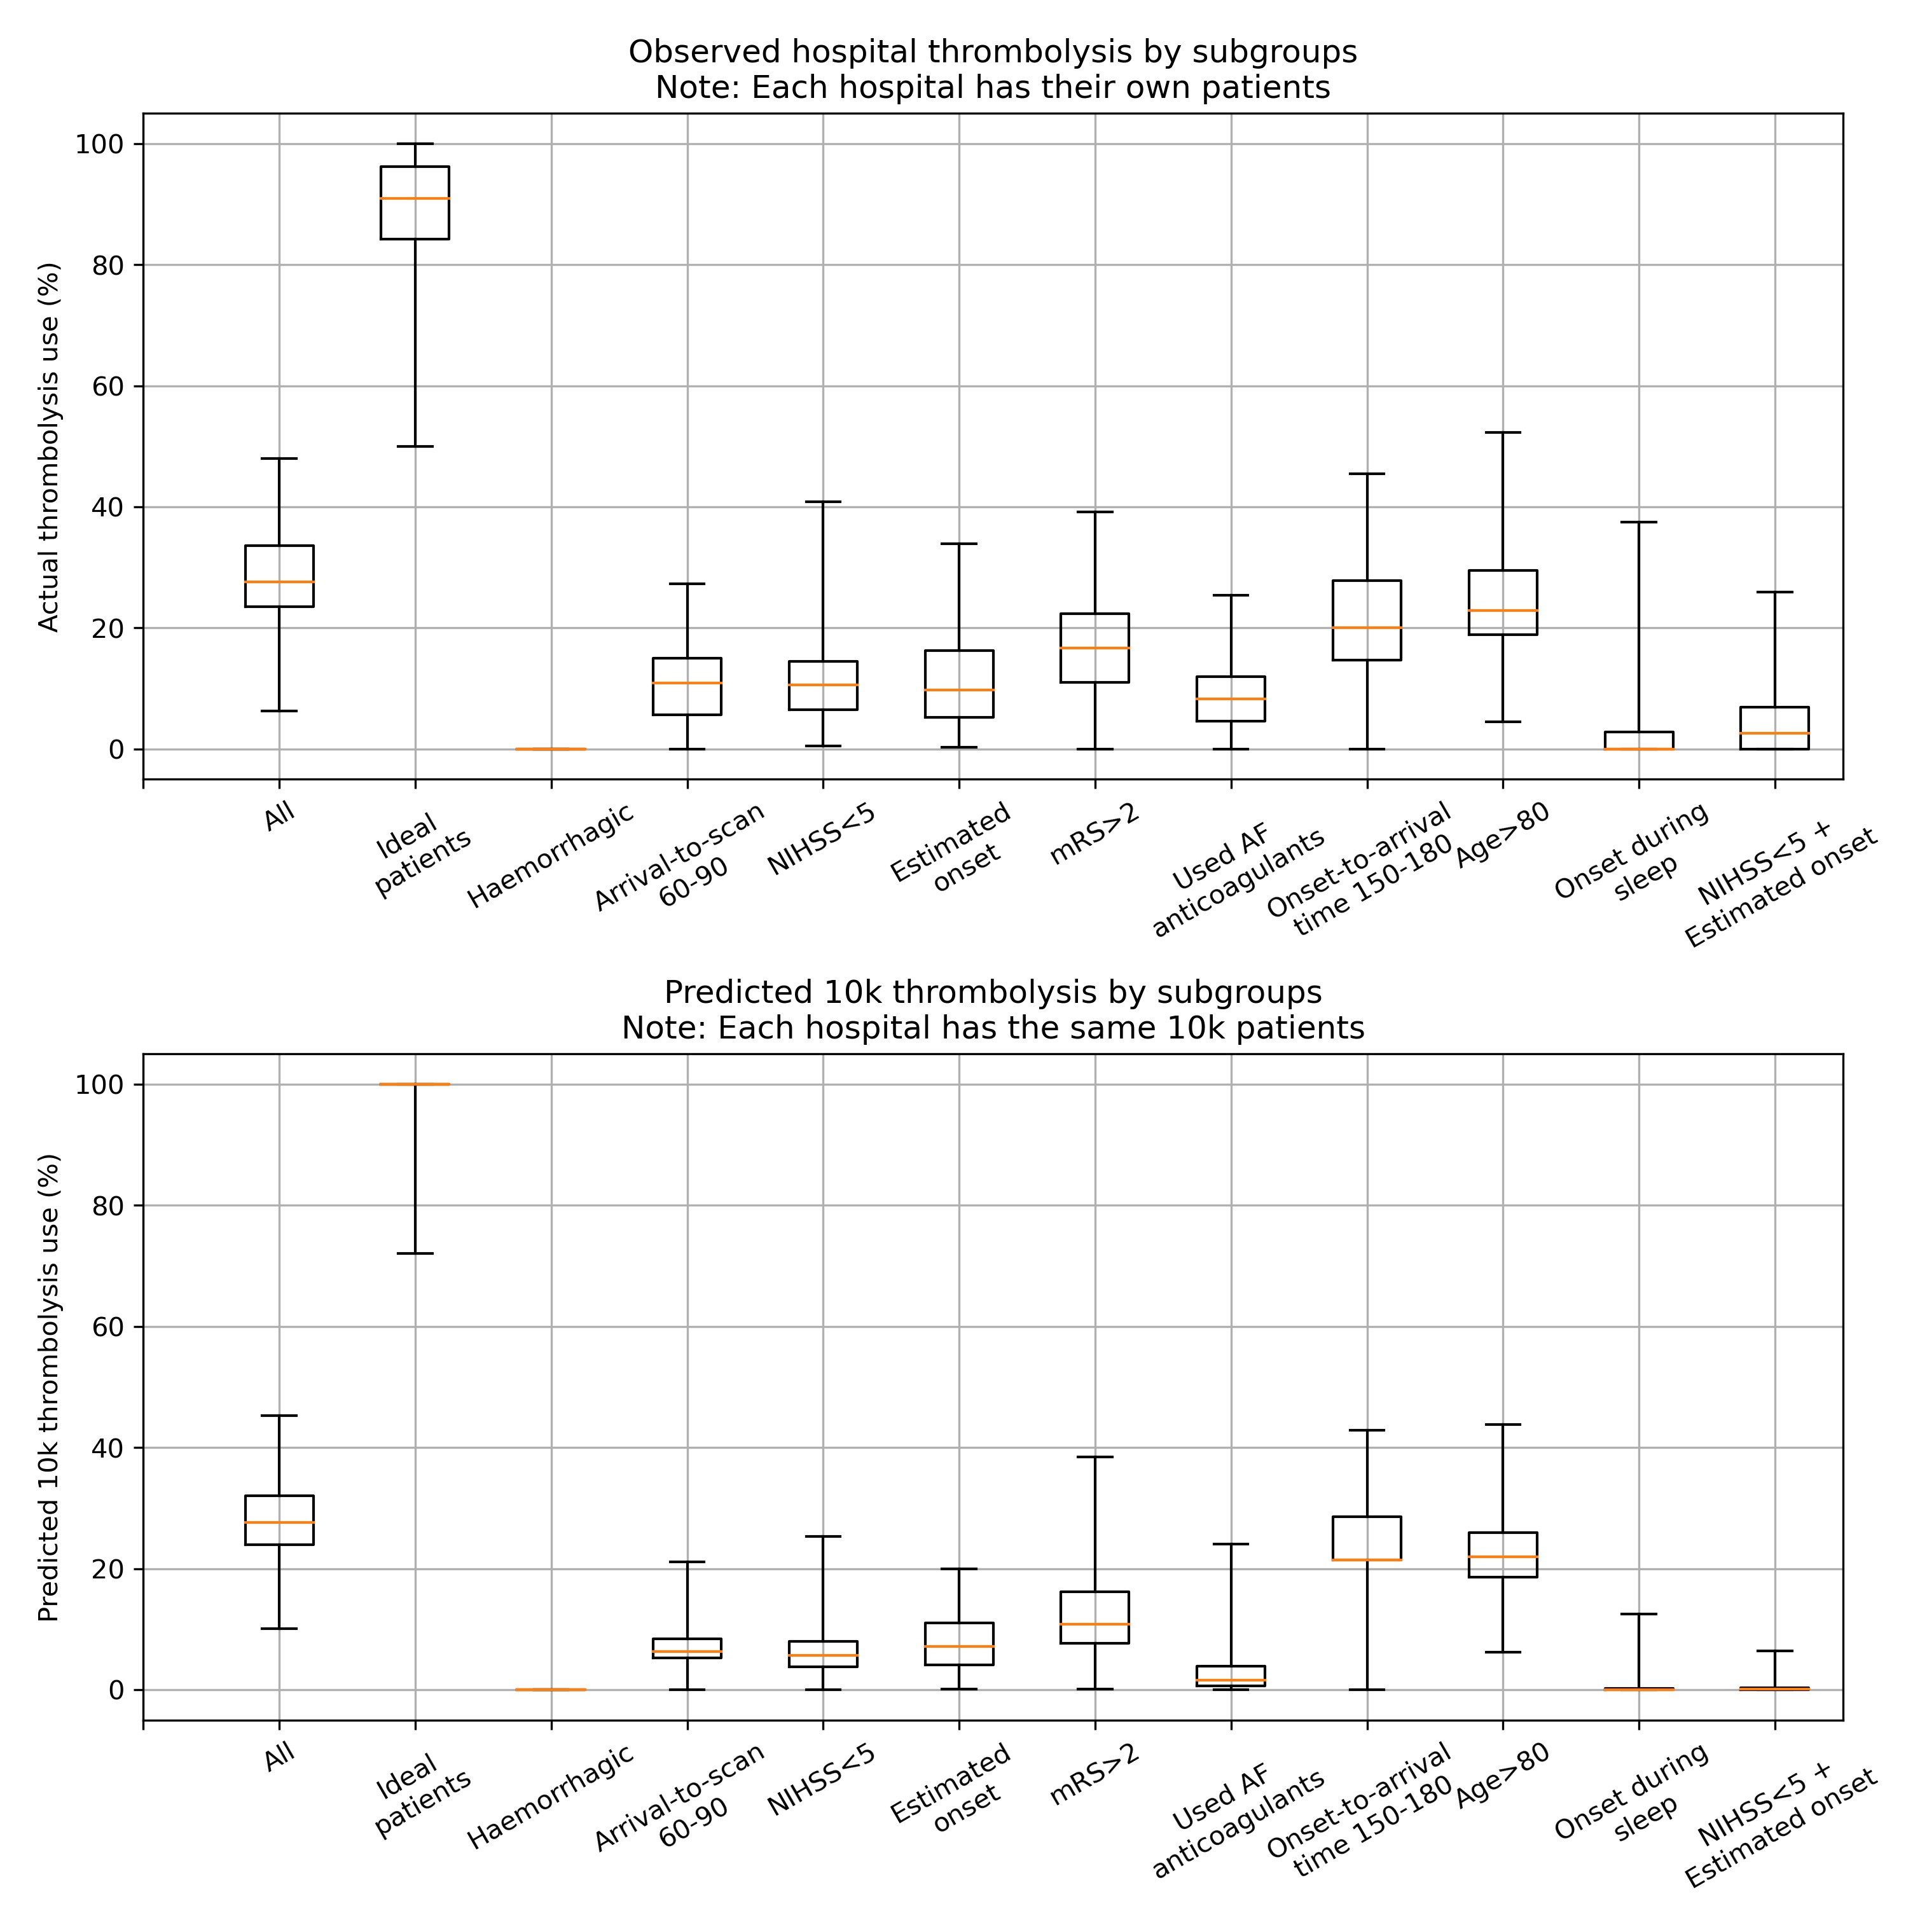
\includegraphics[width=1\textwidth]{./images/15a_xgb_10_features_10k_cohort_actual_vs_modelled_subgroup_boxplot.jpg}%{./images/15a_actual_vs_modelled_subgroup_violin}
\caption{Boxplot for either observed (top) or predicted (bottom) use of thrombolysis for subgroups of patients.}
\label{fig:subgroup_boxplot}
\end{figure}

The observed and predicted subgroup analysis show very similar general patterns (and with a r-squared=0.95, figure \ref{fig:subgroup_correlation}).

\begin{figure}
\centering
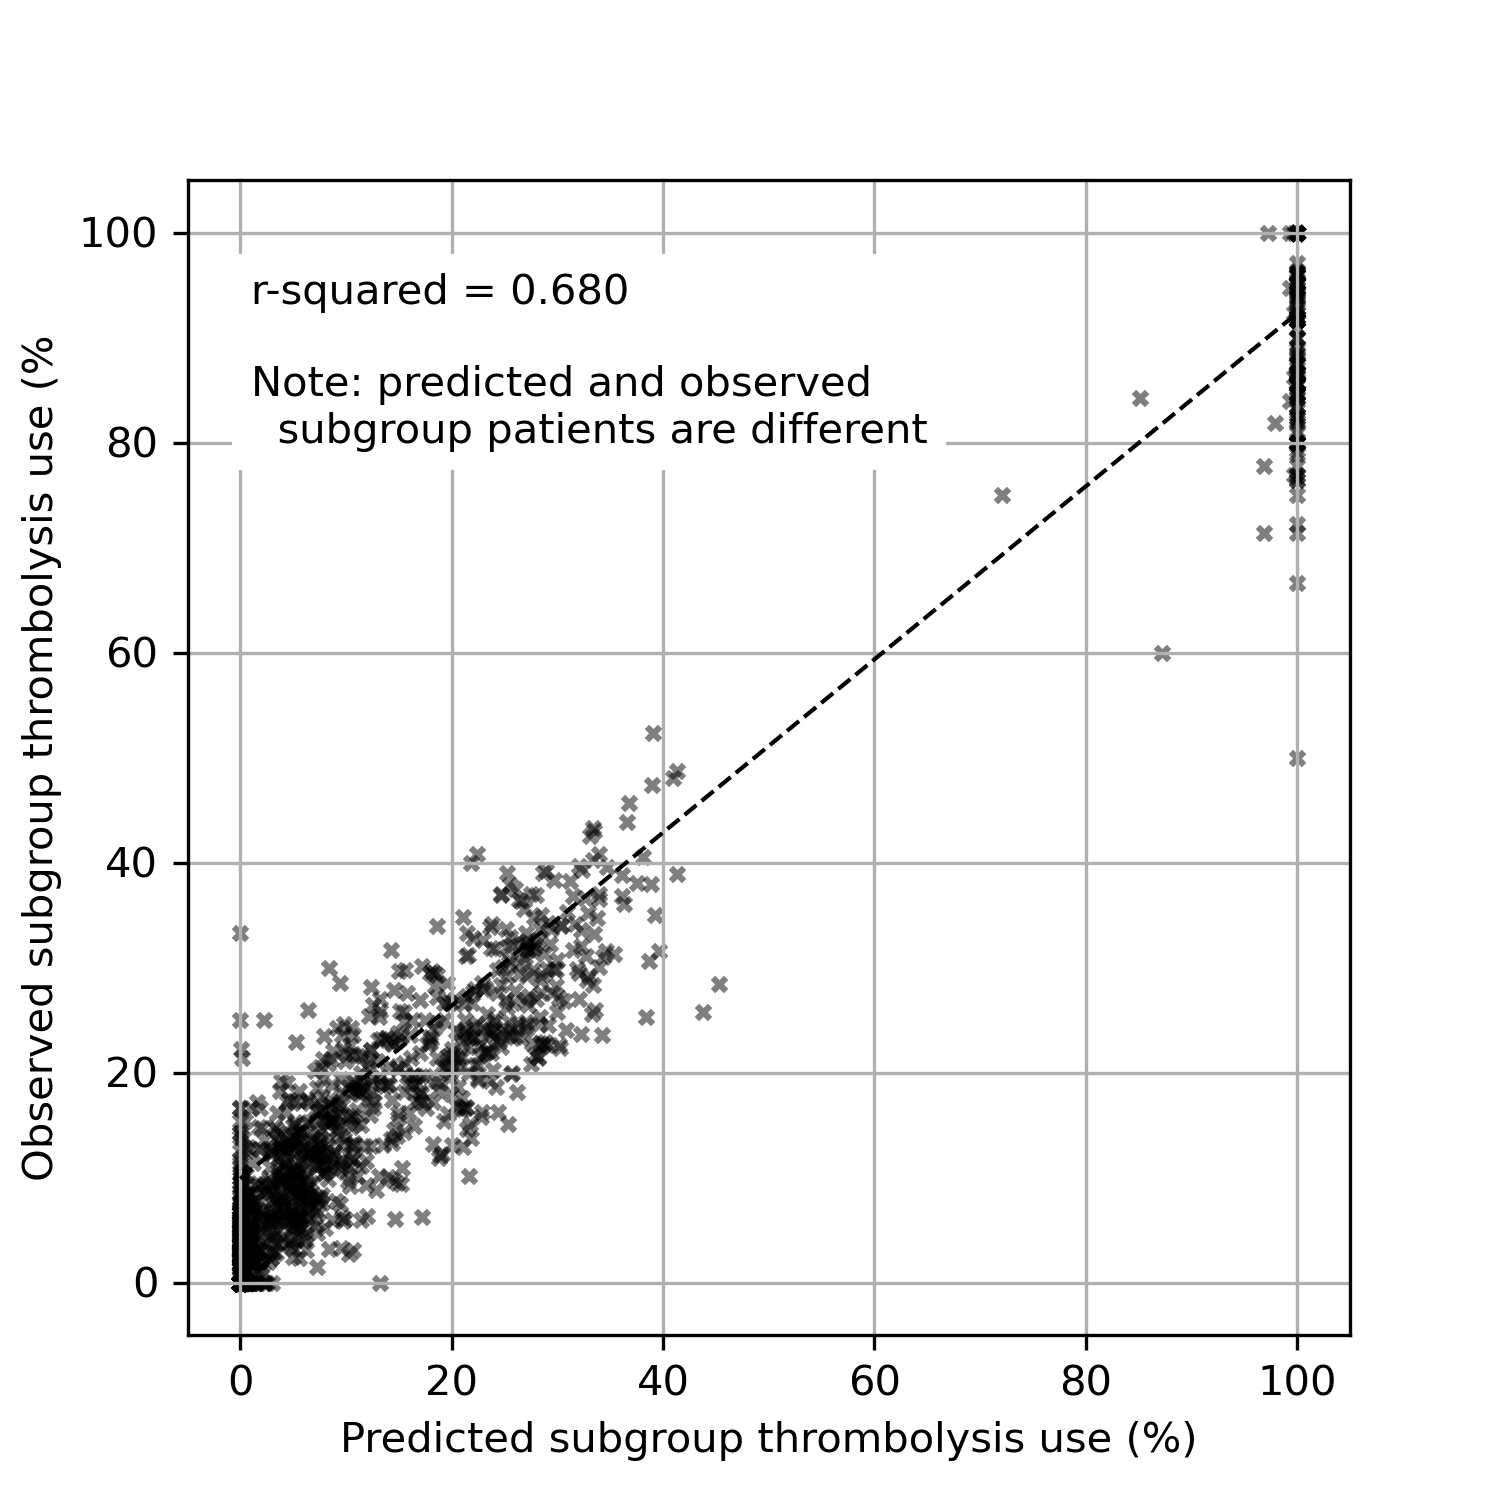
\includegraphics[width=0.7\textwidth]{./images/15a_subgroup_correlation}
\caption{A comparison of predicted and observed use of thrombolysis at each hospital for all subgroups.}
\label{fig:subgroup_correlation}
\end{figure}

The three subgroups of NIHSS $<$5, no precise stroke onset time, and pre-stroke mRS > 2, all had reduced thrombolysis use, and combining these non-ideal features reduced thrombolysis use further.

Some differences existed:

\begin{itemize}
    \item The use of thrombolysis in *ideal* patients is a little low in the observed vs actual results (mean hospital thrombolysis use = 89\% vs 99\%).
    \item The predicted results show a stronger effect of combining non-ideal features.
    \item The observed thrombolysis rate shows higher between-hospital variation than the predicted thrombolysis rate. This may be partly explained by the observed thrombolysis rate being on different patients at each hospital, but may also be partly explained by actual use of thrombolysis being slightly more variable than predicted thrombolysis use (which will follow general hospital patterns, and will not include, for example, between-clinician variation at each hospital).
\end{itemize}

When we look at observed thrombolysis use in subgroups at each hospital we see that the thrombolysis use across the subgroups tended to reduce in parallel (figure \ref{fig:subgroup_rate_1} r-squared 0.221 - 0.680 in observed thrombolysis use, and 0.445 to 0.868 in the predicted thrombolysis use), along with thrombolysis use for all patients, suggesting a  caution in use of thrombolysis in all subgroups of 'less than ideal' patients. 

\begin{figure}
\centering
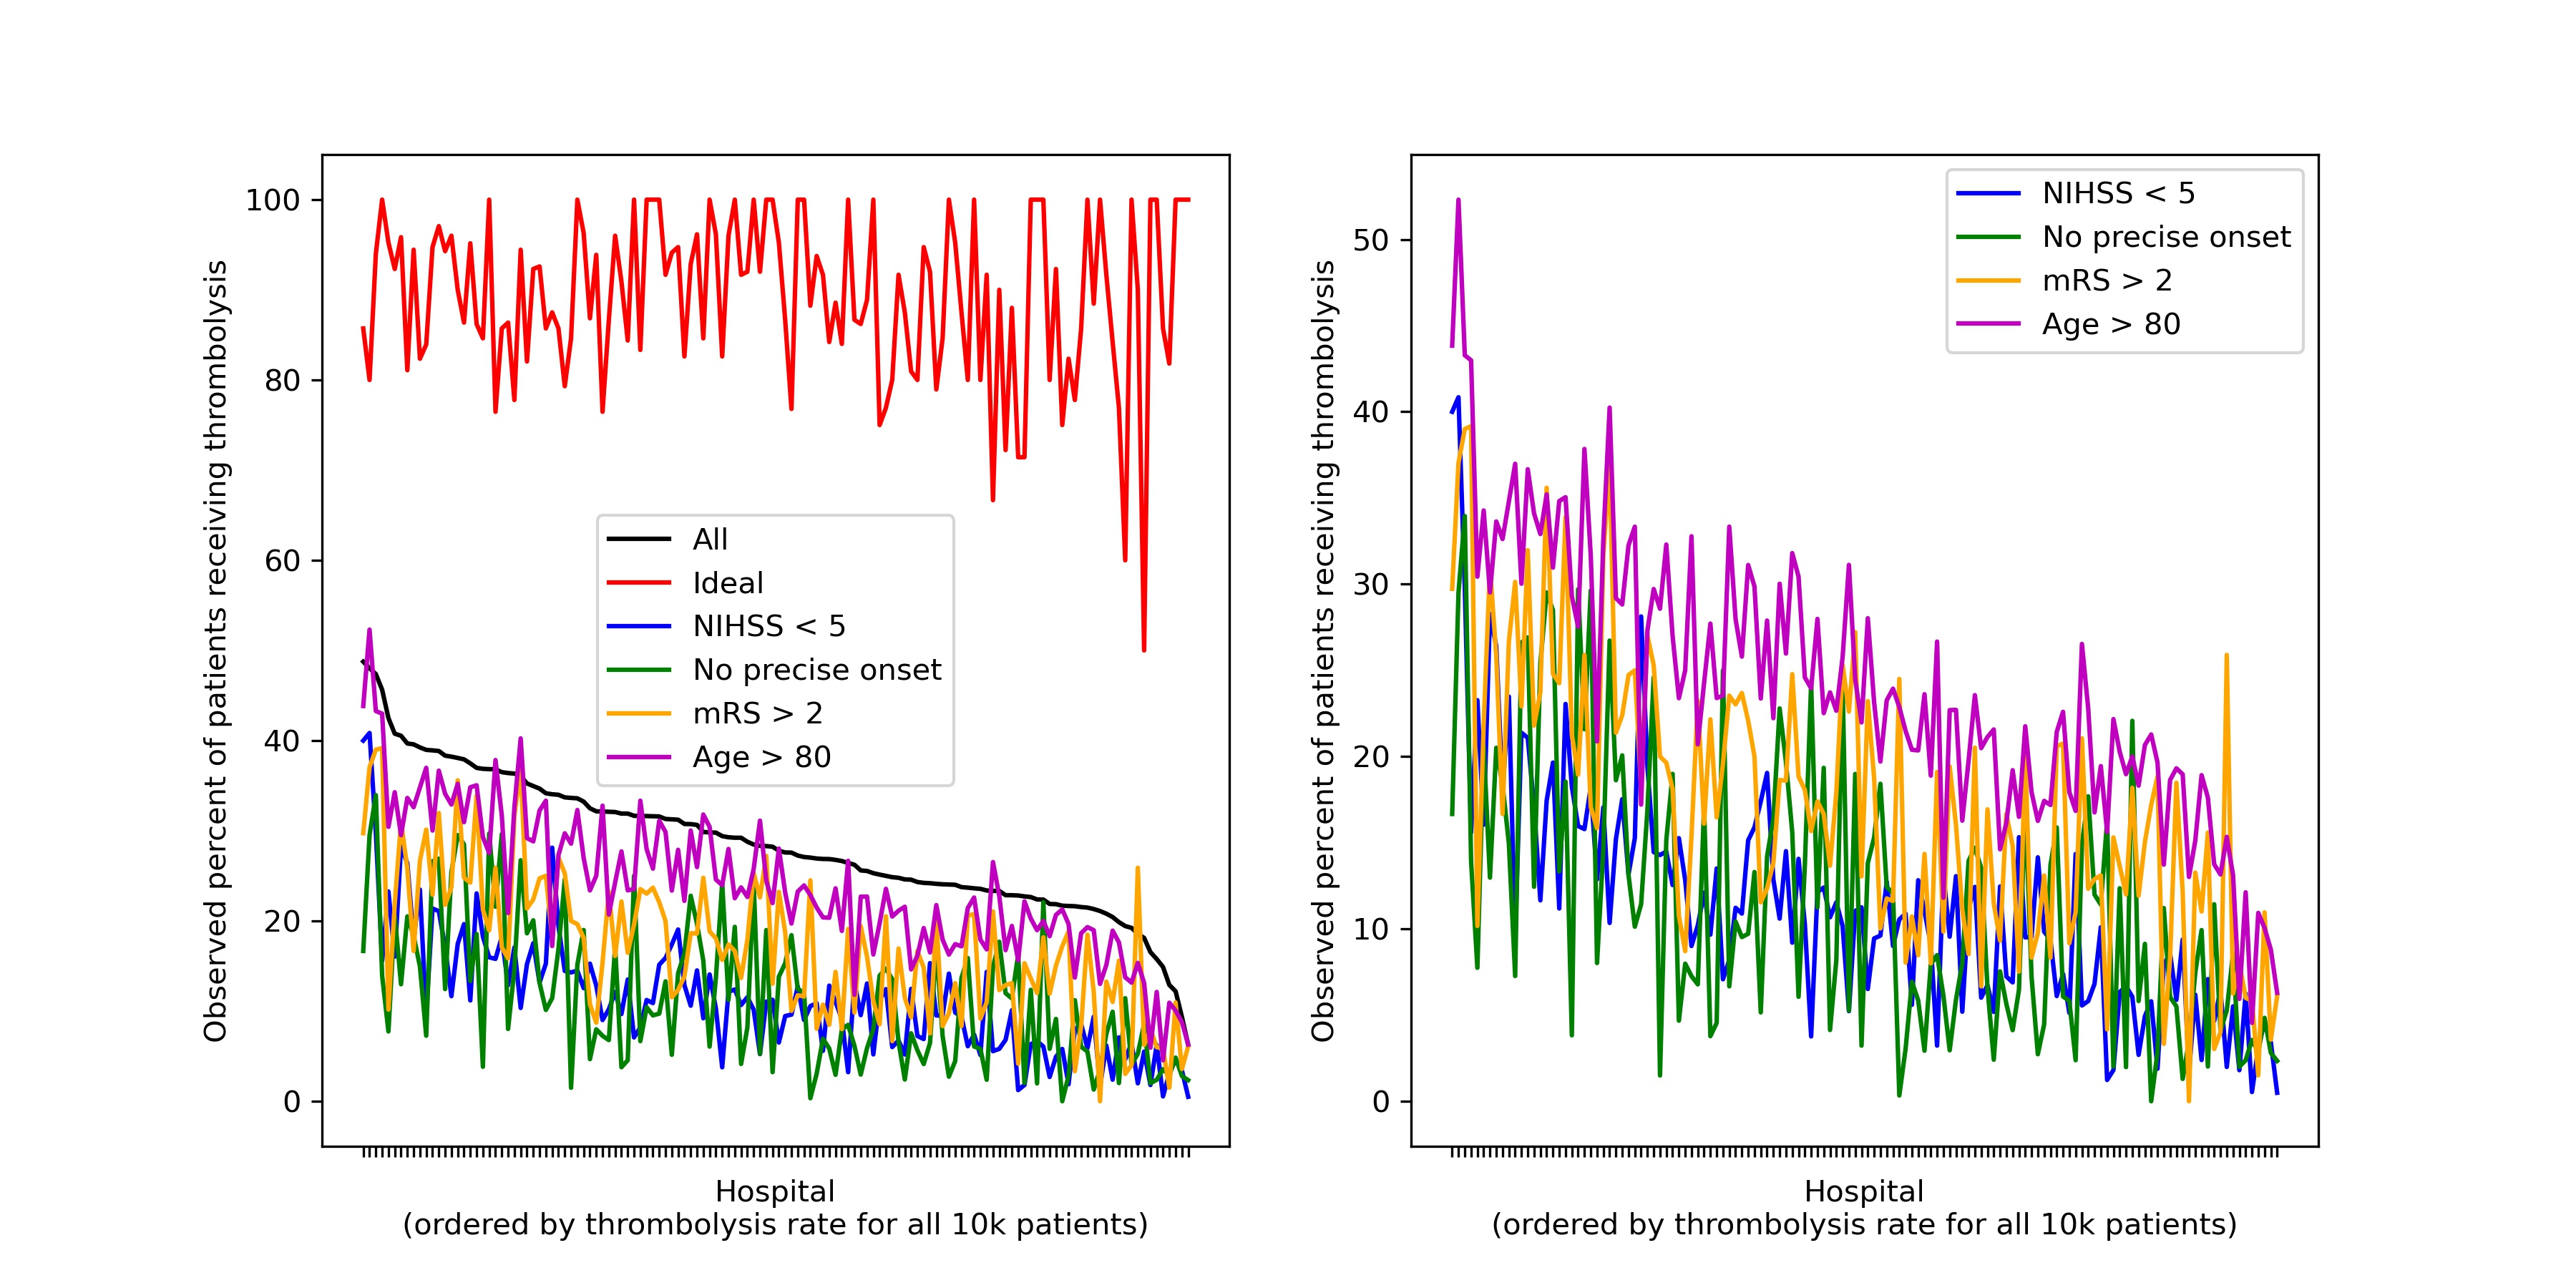
\includegraphics[width=1\textwidth]{./images/15a_actual_subgroup}
\caption{Observed thrombolysis use for all patients and subgroups of patients at each of 132 hospitals, with hospitals ordered by descending thrombolysis use of all patients. Results are for all patients attending each hospital.}
\label{fig:subgroup_rate_1}
\end{figure}

This parallel reduction in use of thrombolysis across the subgroups was also seen in the predicted use of thrombolysis in the 10k cohort of patients (figure \ref{fig:subgroup_rate_2}).

\begin{figure}
\centering
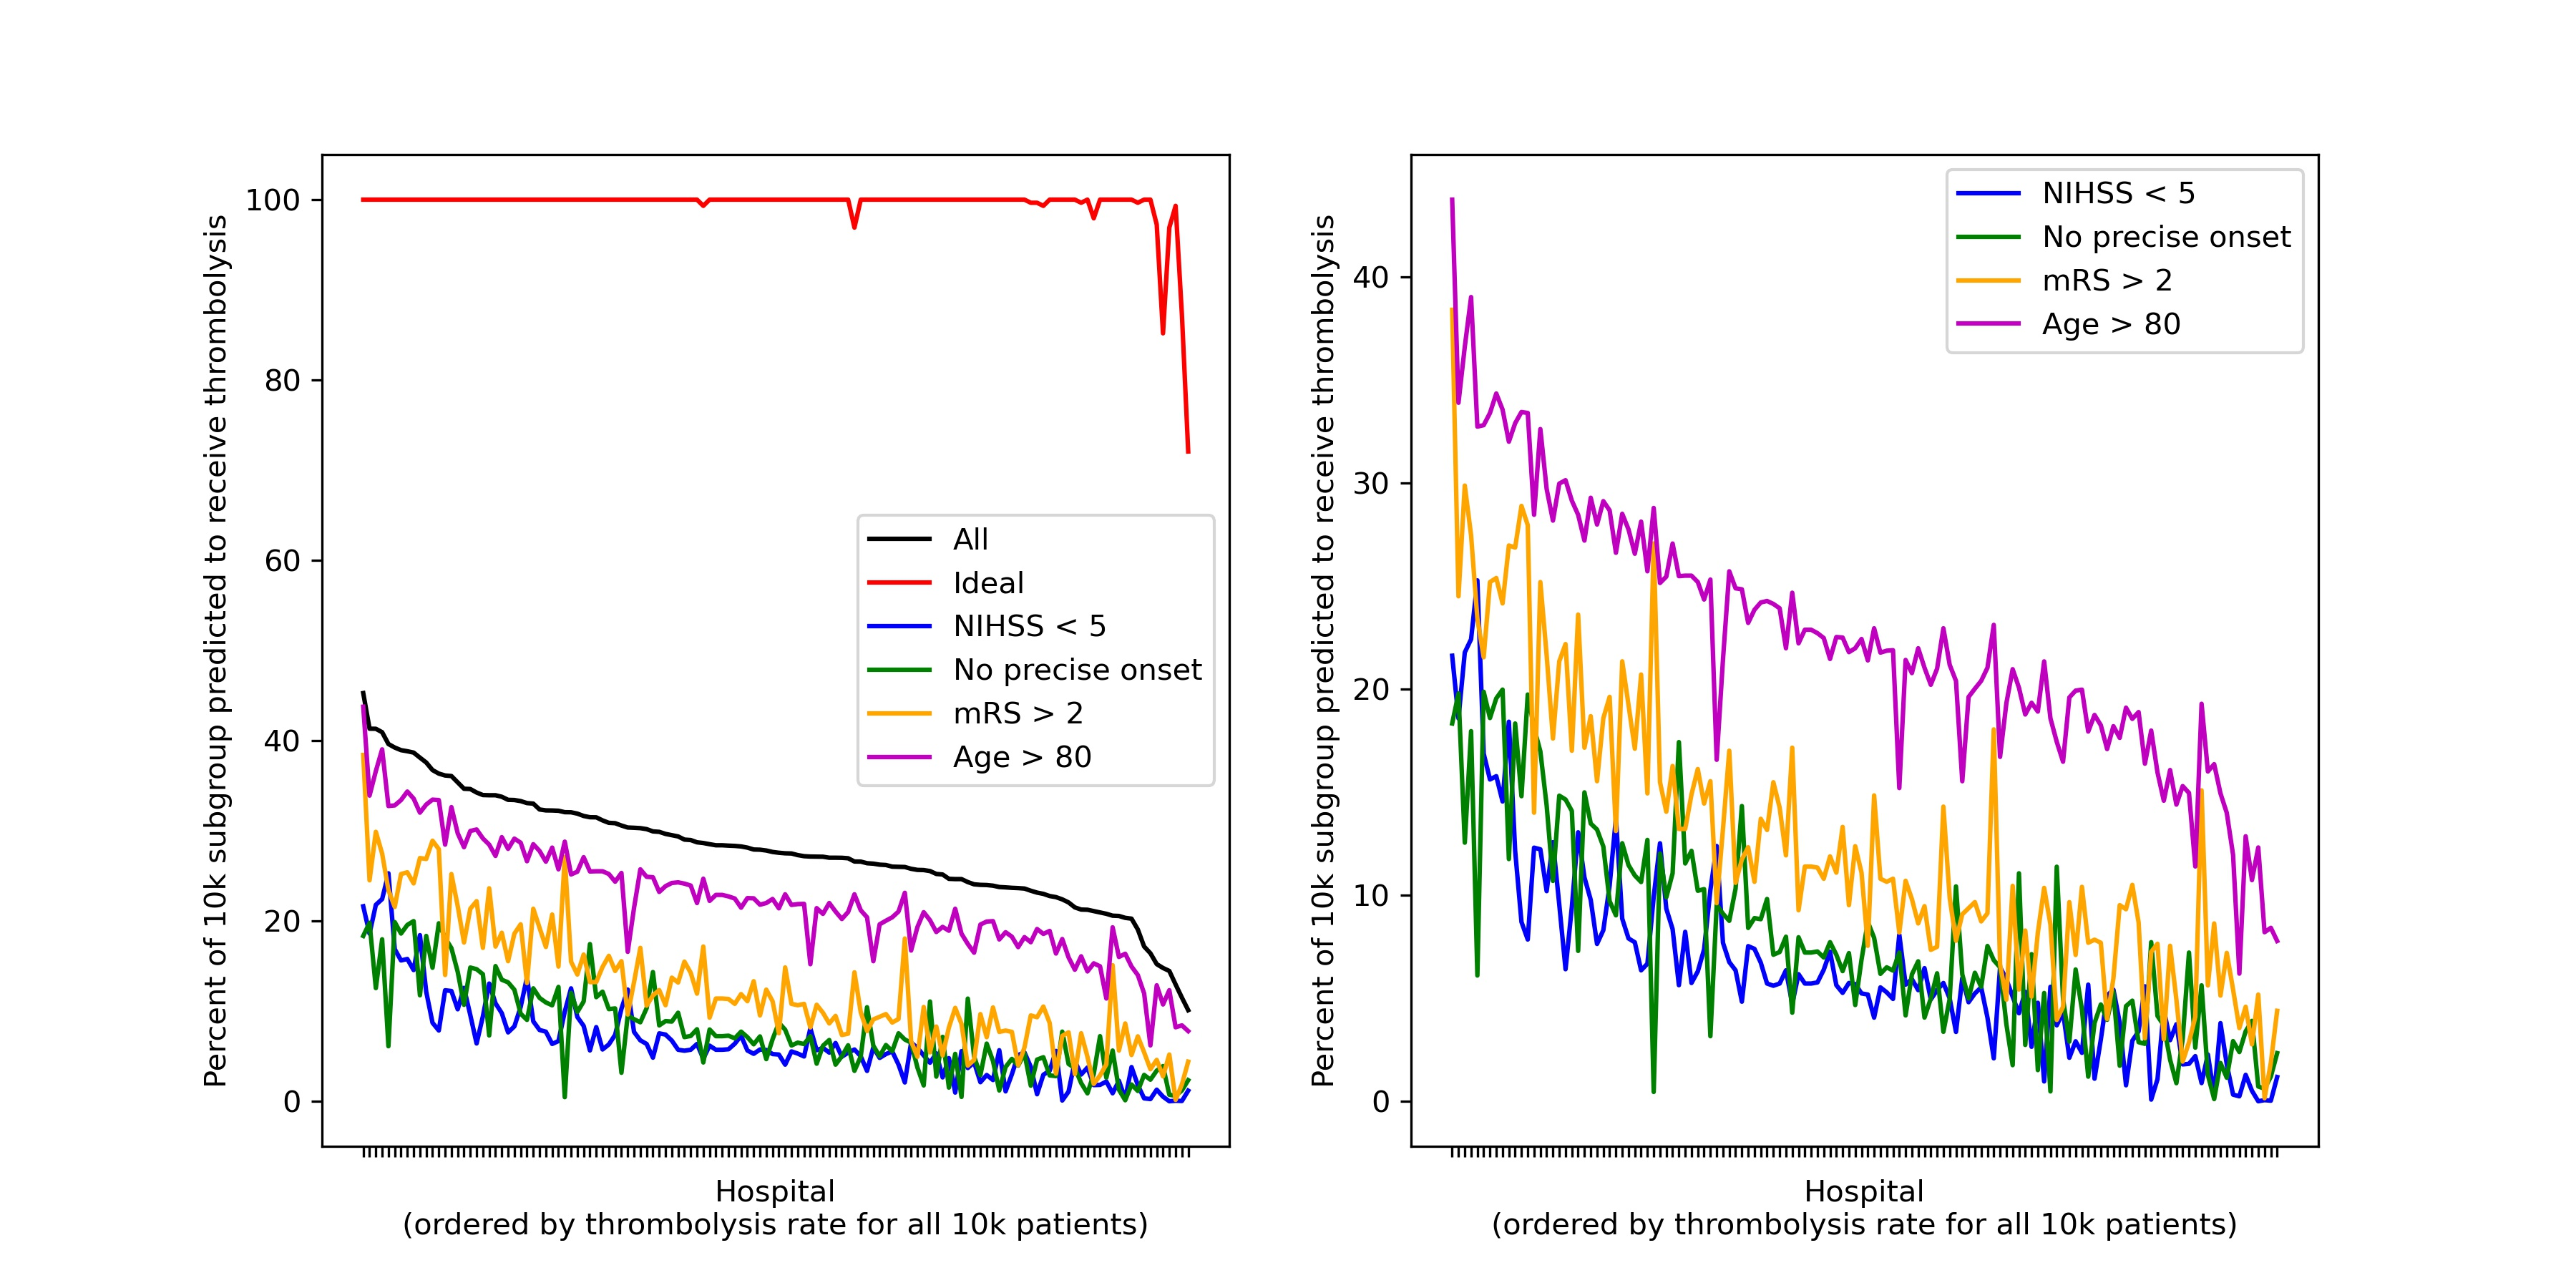
\includegraphics[width=1\textwidth]{./images/15_10k_subgroup}
\caption{Predicted thrombolysis use for all patients and subgroups of patients at each of 132 hospitals, with hospitals ordered by descending thrombolysis use of all patients. Results are based on a prediction of thrombolysis in a 10k cohort of patients}
\label{fig:subgroup_rate_2}
\end{figure}

%%%%%%%%%%%%%%%%%%%%%%%%%%%%%%%%%%%%%%%%%%%%%%%%%%%%%%%%%%%%%%%%%%%%%%%%%%%%%%%%%%%%%%%

\subsection{A comparison of thrombolysis use in high and low thrombolysing units by feature values}

We investigated the relationships between feature values and thrombolysis use for low and high thrombolysing hospitals (figure \ref{fig:thrombolysis_by_feature_value}). The high and low thrombolysing hospitals were taken as the top and bottom 30 hospitals as ranked by the predicted thrombolysis use in the same 10k cohort of patients. We found that thrombolysis use in low thrombolysing hospitals followed the same general relationship with feature values as the high thrombolysing hospitals, but thrombolysis was consistently lower.

\begin{figure}
\centering
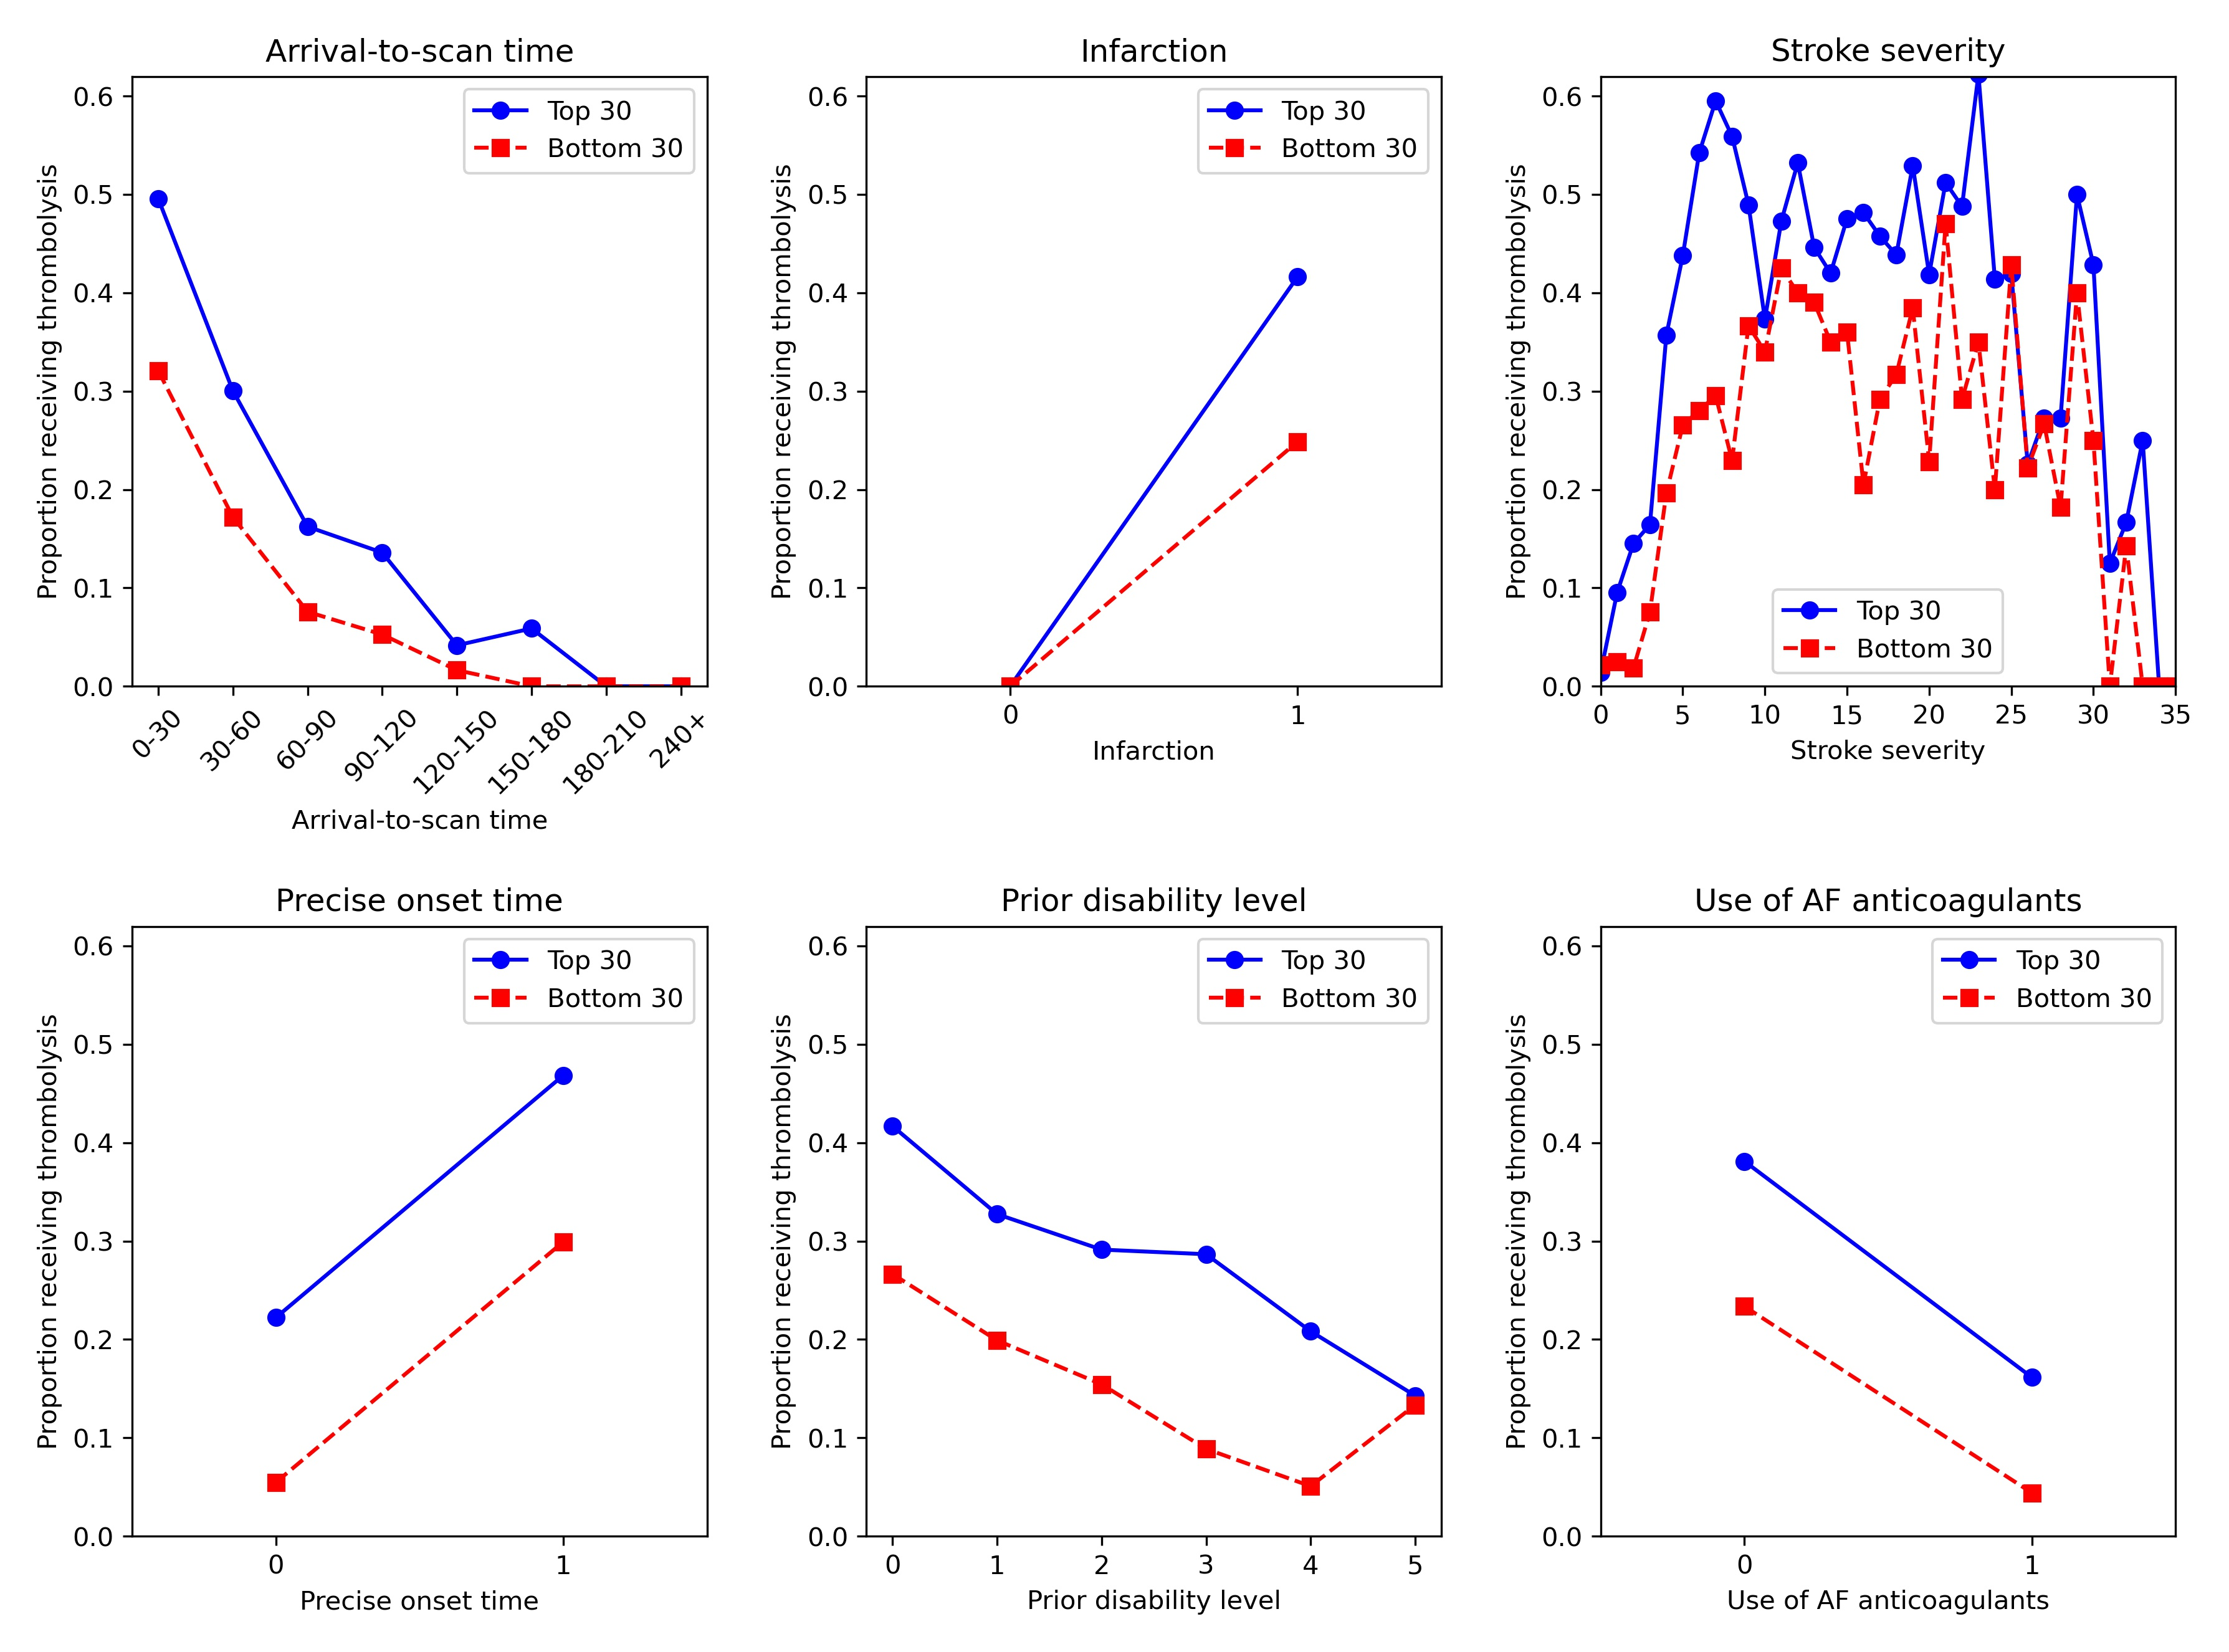
\includegraphics[width=1\textwidth]{./images/09_compare_thrombolysis_by_feature}
\caption{Observed use of thrombolysis by feature value in the top (blue) and bottom (red) 30 thrombolysing hospitals as assessed by predicted thrombolysis use in a 10k cohort of patients.}
\label{fig:thrombolysis_by_feature_value}
\end{figure}

%%%%%%%%%%%%%%%%%%%%%%%%%%%%%%%%%%%%%%%%%%%%%%%%%%%%%%%%%%%%%%%%%%%%%%%%%%%%%%%%%%%%%%%

\subsection{Artificial patients}

We used artificial patients to investigate controlled changes to patients, to see how many hospitals were predicted to give thrombolysis.

We started with a 'base patient' who had features that are favourable to use of thrombolysis:

\begin{itemize}
\item Onset to arrival = 80 mins
\item Arrival to scan = 20 mins
\item Infarction = 1
\item NIHSS = 15
\item Prior disability level = 0
\item Precise onset time = 1
\item Use of AF anticoagulants = 0
\end{itemize}

We then varied the following features in turn, keeping all other features
the same as the base patient:

\begin{itemize}
\item NIHSS = 0-40
\item Prior disability level = 0-5
\item Precise onset time = 0-1
\end{itemize}

The number of hospitals giving predicted to give thrombolysis to these alternative artificial patients was:

\begin{itemize}
\item Base patient: 132 (99\%)
\item As base patient, but NIHSS = 5: 123 (93\%)
\item As base patient, but pre-stroke disability = 2: 125 (95\%)
\item As base patient, but estimated stroke onset time: 109 (83\%)
\end{itemize}

Combining two marginal features:

\begin{itemize}
\item As base patient, but NIHSS = 5 and pre-stroke disability = 2: 78 (59\%)
\item As base patient, but NIHSS = 5 and estimated stroke onset time: 30 (23\%)
\item As base patient, but pre-stroke disability = 2 and estimated stroke onset time: 26 (20\%)
\end{itemize}

Combining three marginal features:

\begin{itemize}
\item As base patient, but NIHSS = 5, pre-stroke disability = 2, estimated stroke onset time: 2 (1.5\%)
\end{itemize}

Starting with the ideal patient, and changing only feature at a time we investigated changing stroke severity, pre-stroke disability, and precise onset time (figure \ref{fig:artificial_1}).

\begin{figure}
\centering
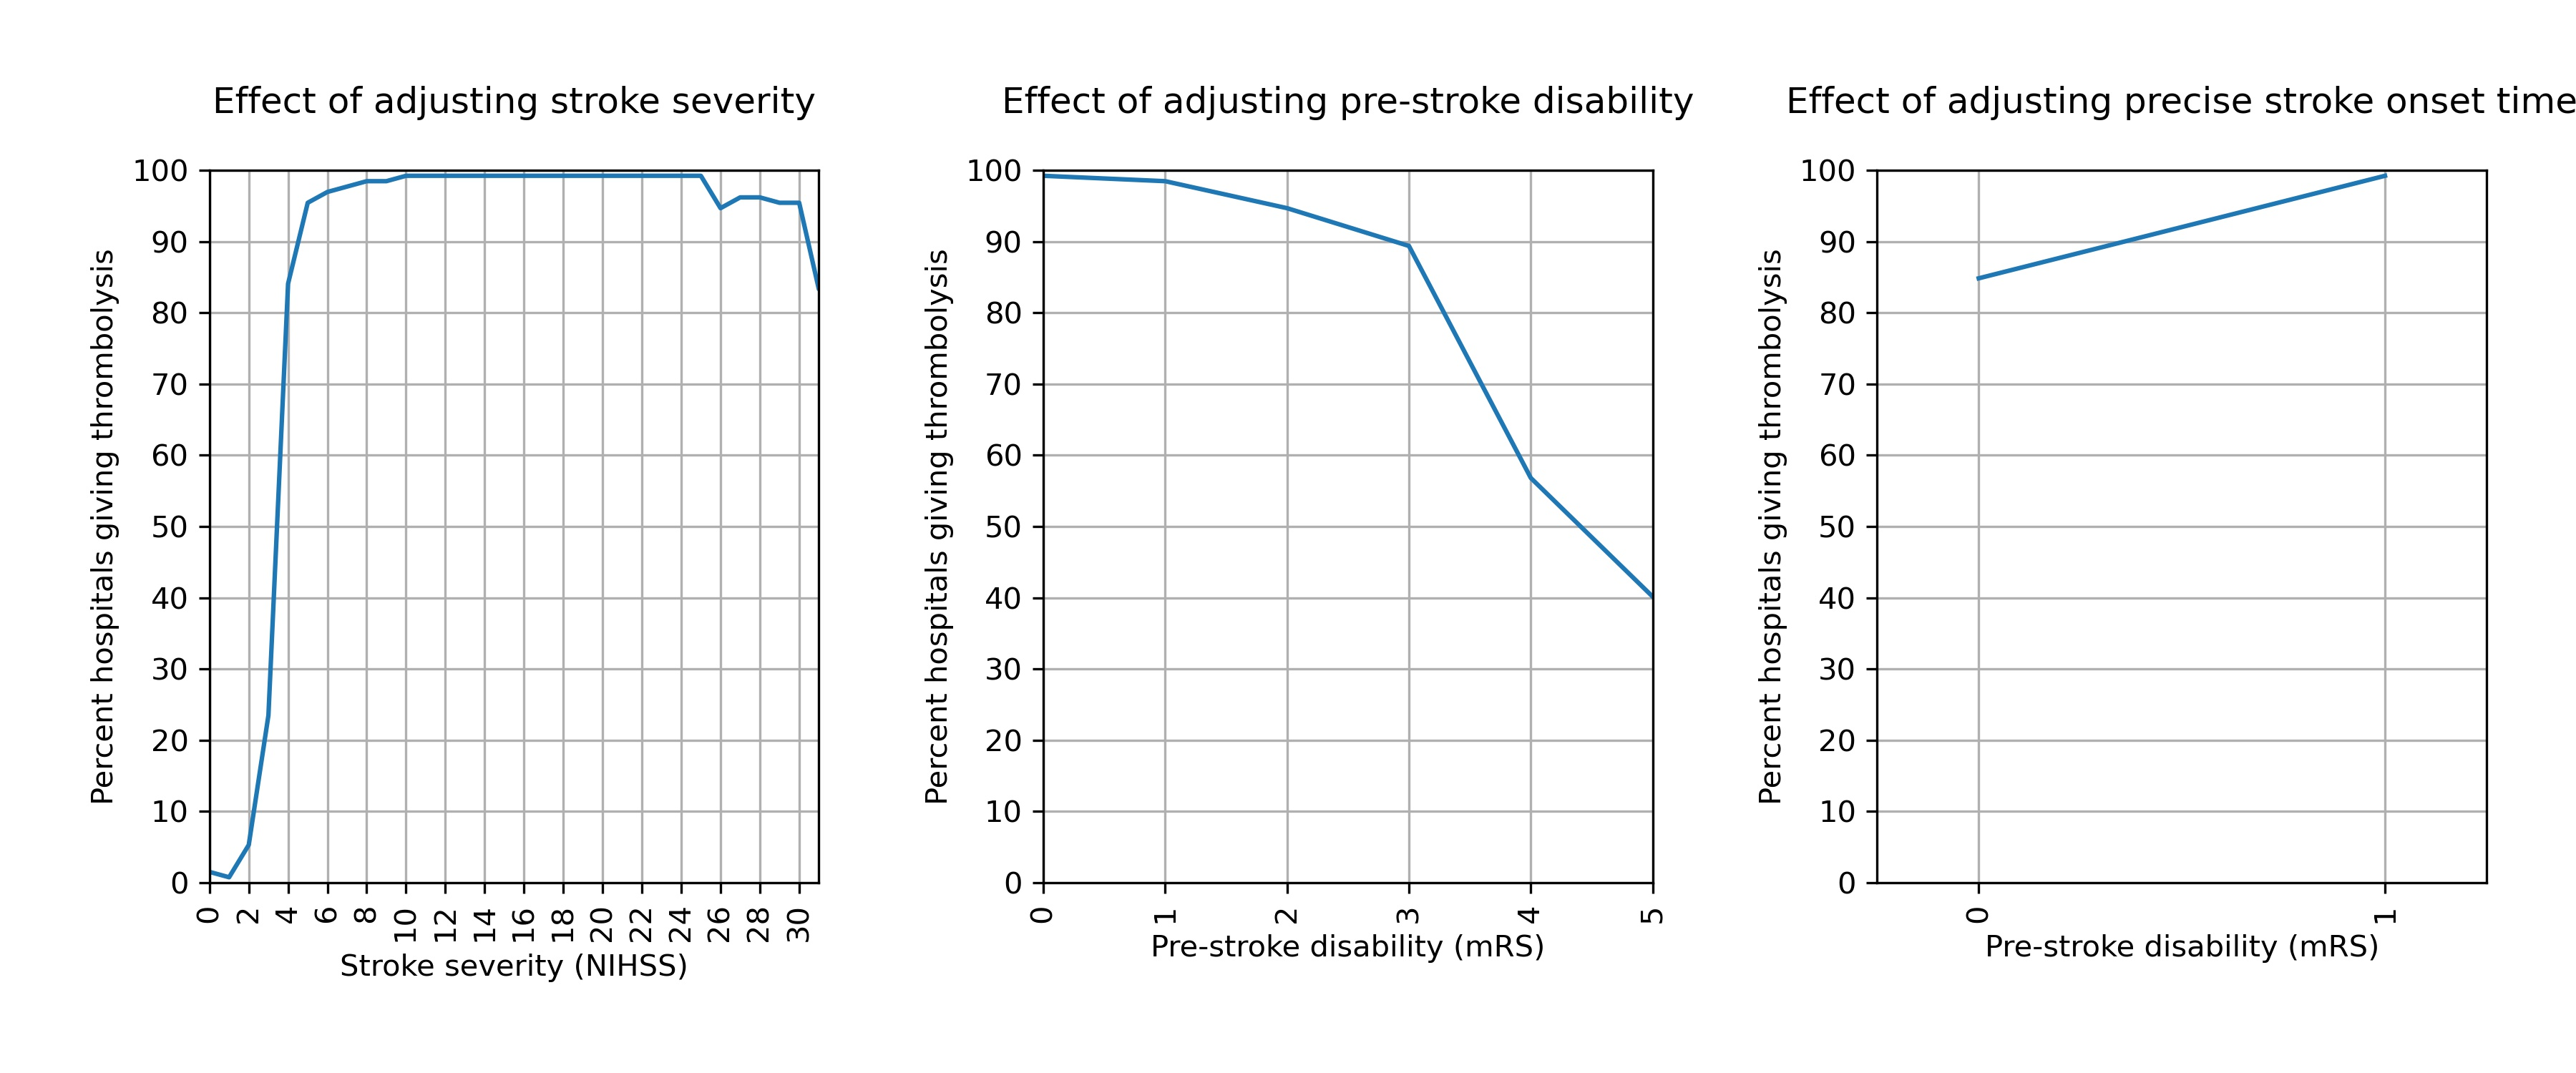
\includegraphics[width=1\textwidth]{./images/20_synthetic_xgb_10_features_IVT_rate_vs_feature_values}
\caption{The effect of changing stroke severity, pre-stroke disability, or precise onset time on the proportion of hospitals that would be expected to give thrombolysis to a patient. Patients otherwise have the following feature values: Onset to arrival = 80 mins, Arrival to scan = 20 mins, Infarction = 1, NIHSS = 15, Prior disability level = 0, Precise onset time = 1, Use of AF anticoagulants = 0.}
\label{fig:artificial_1}
\end{figure}

Figure \ref{fig:artificial_shap_waterfall_with_violin} shows SHAP waterfall plots for the same patient attending each of 132 hospitals.

\begin{figure}
\centering
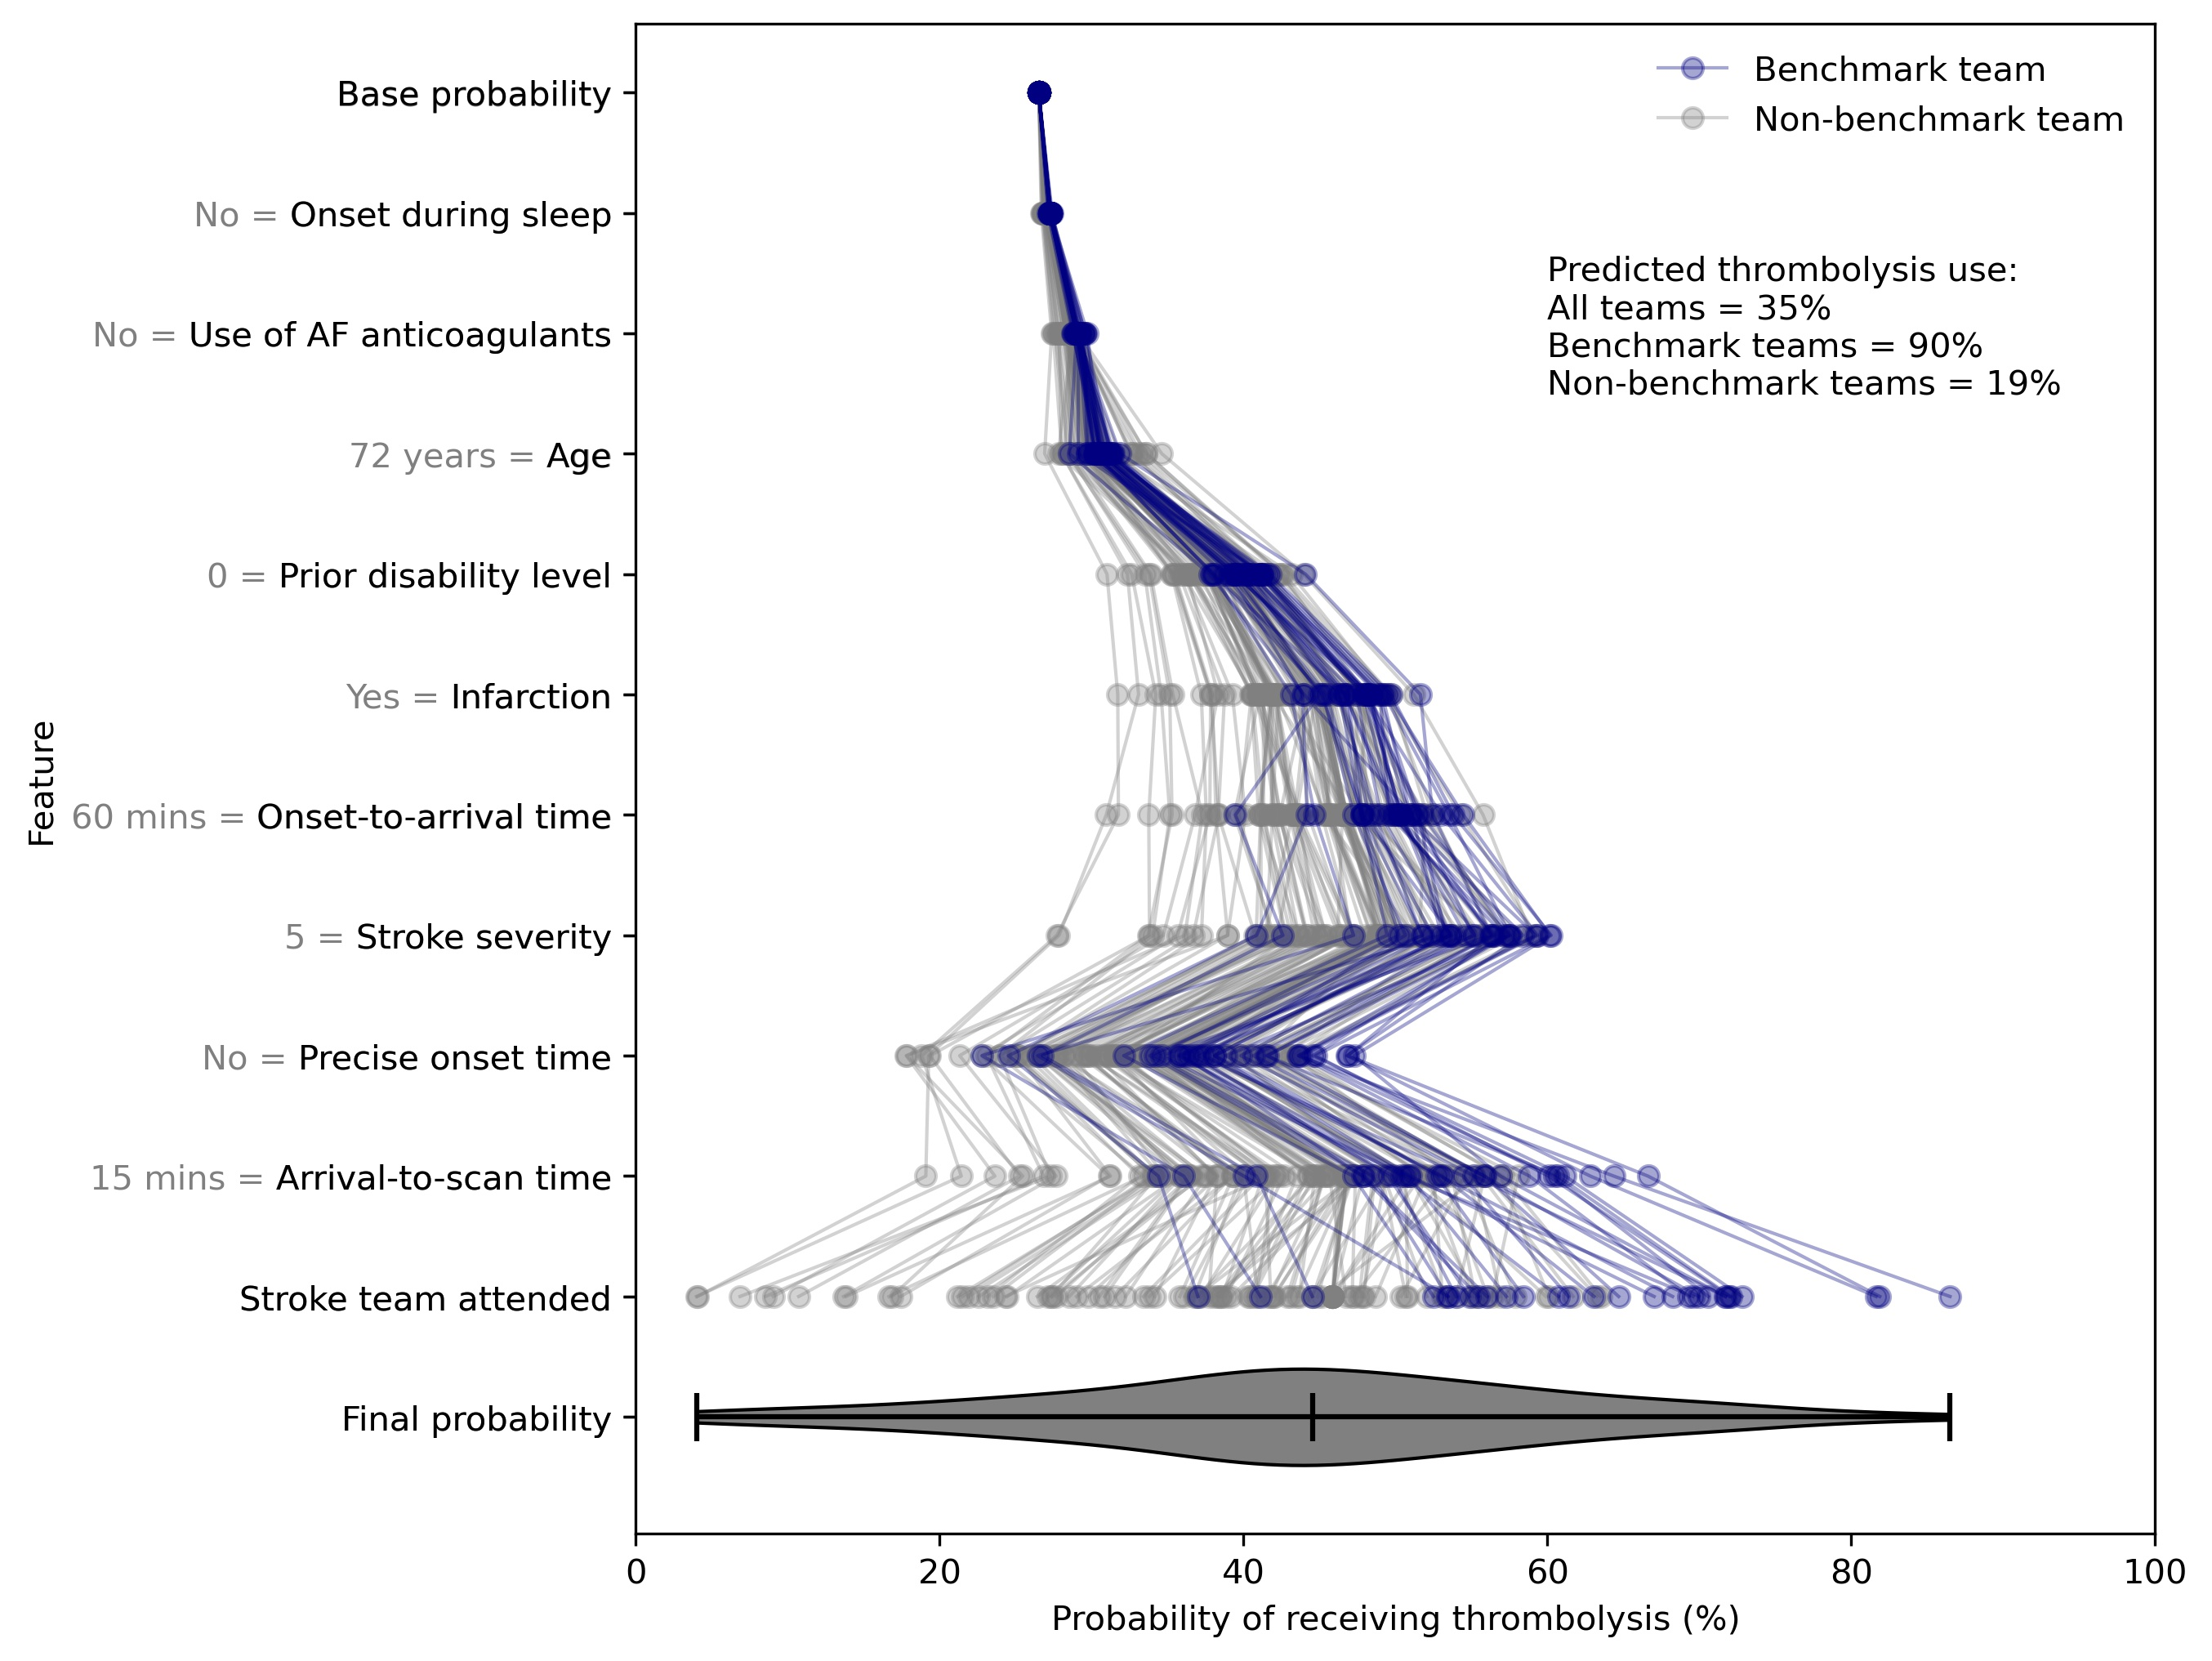
\includegraphics[width=0.7\textwidth]{./images/21_shap_waterfall_with_violin_contentious}
\caption{SHAP waterfall plots for the same patient attending 132 different hospitals. The patient has the following feature values: Onset to arrival = 80 mins, Arrival to scan = 20 mins, Infarction = 1, NIHSS = 5, Prior disability level = 0, Precise onset time = 0, Use of AF anticoagulants = 0.}
\label{fig:artificial_shap_waterfall_with_violin}
\end{figure}


We also studied combining changes to the patient (starting with the 'ideal' thrombolysable patient). Figure \ref{fig:artificial_2} shows the proportion of hospitals predicted to give a patient thrombolysis by altering stroke severity in combination with estimated (non-precise) onset time, mild pre-existing disability (mRS 2), or a combination of estimated onset time and mild pre-existing disability.

\begin{figure}
\centering
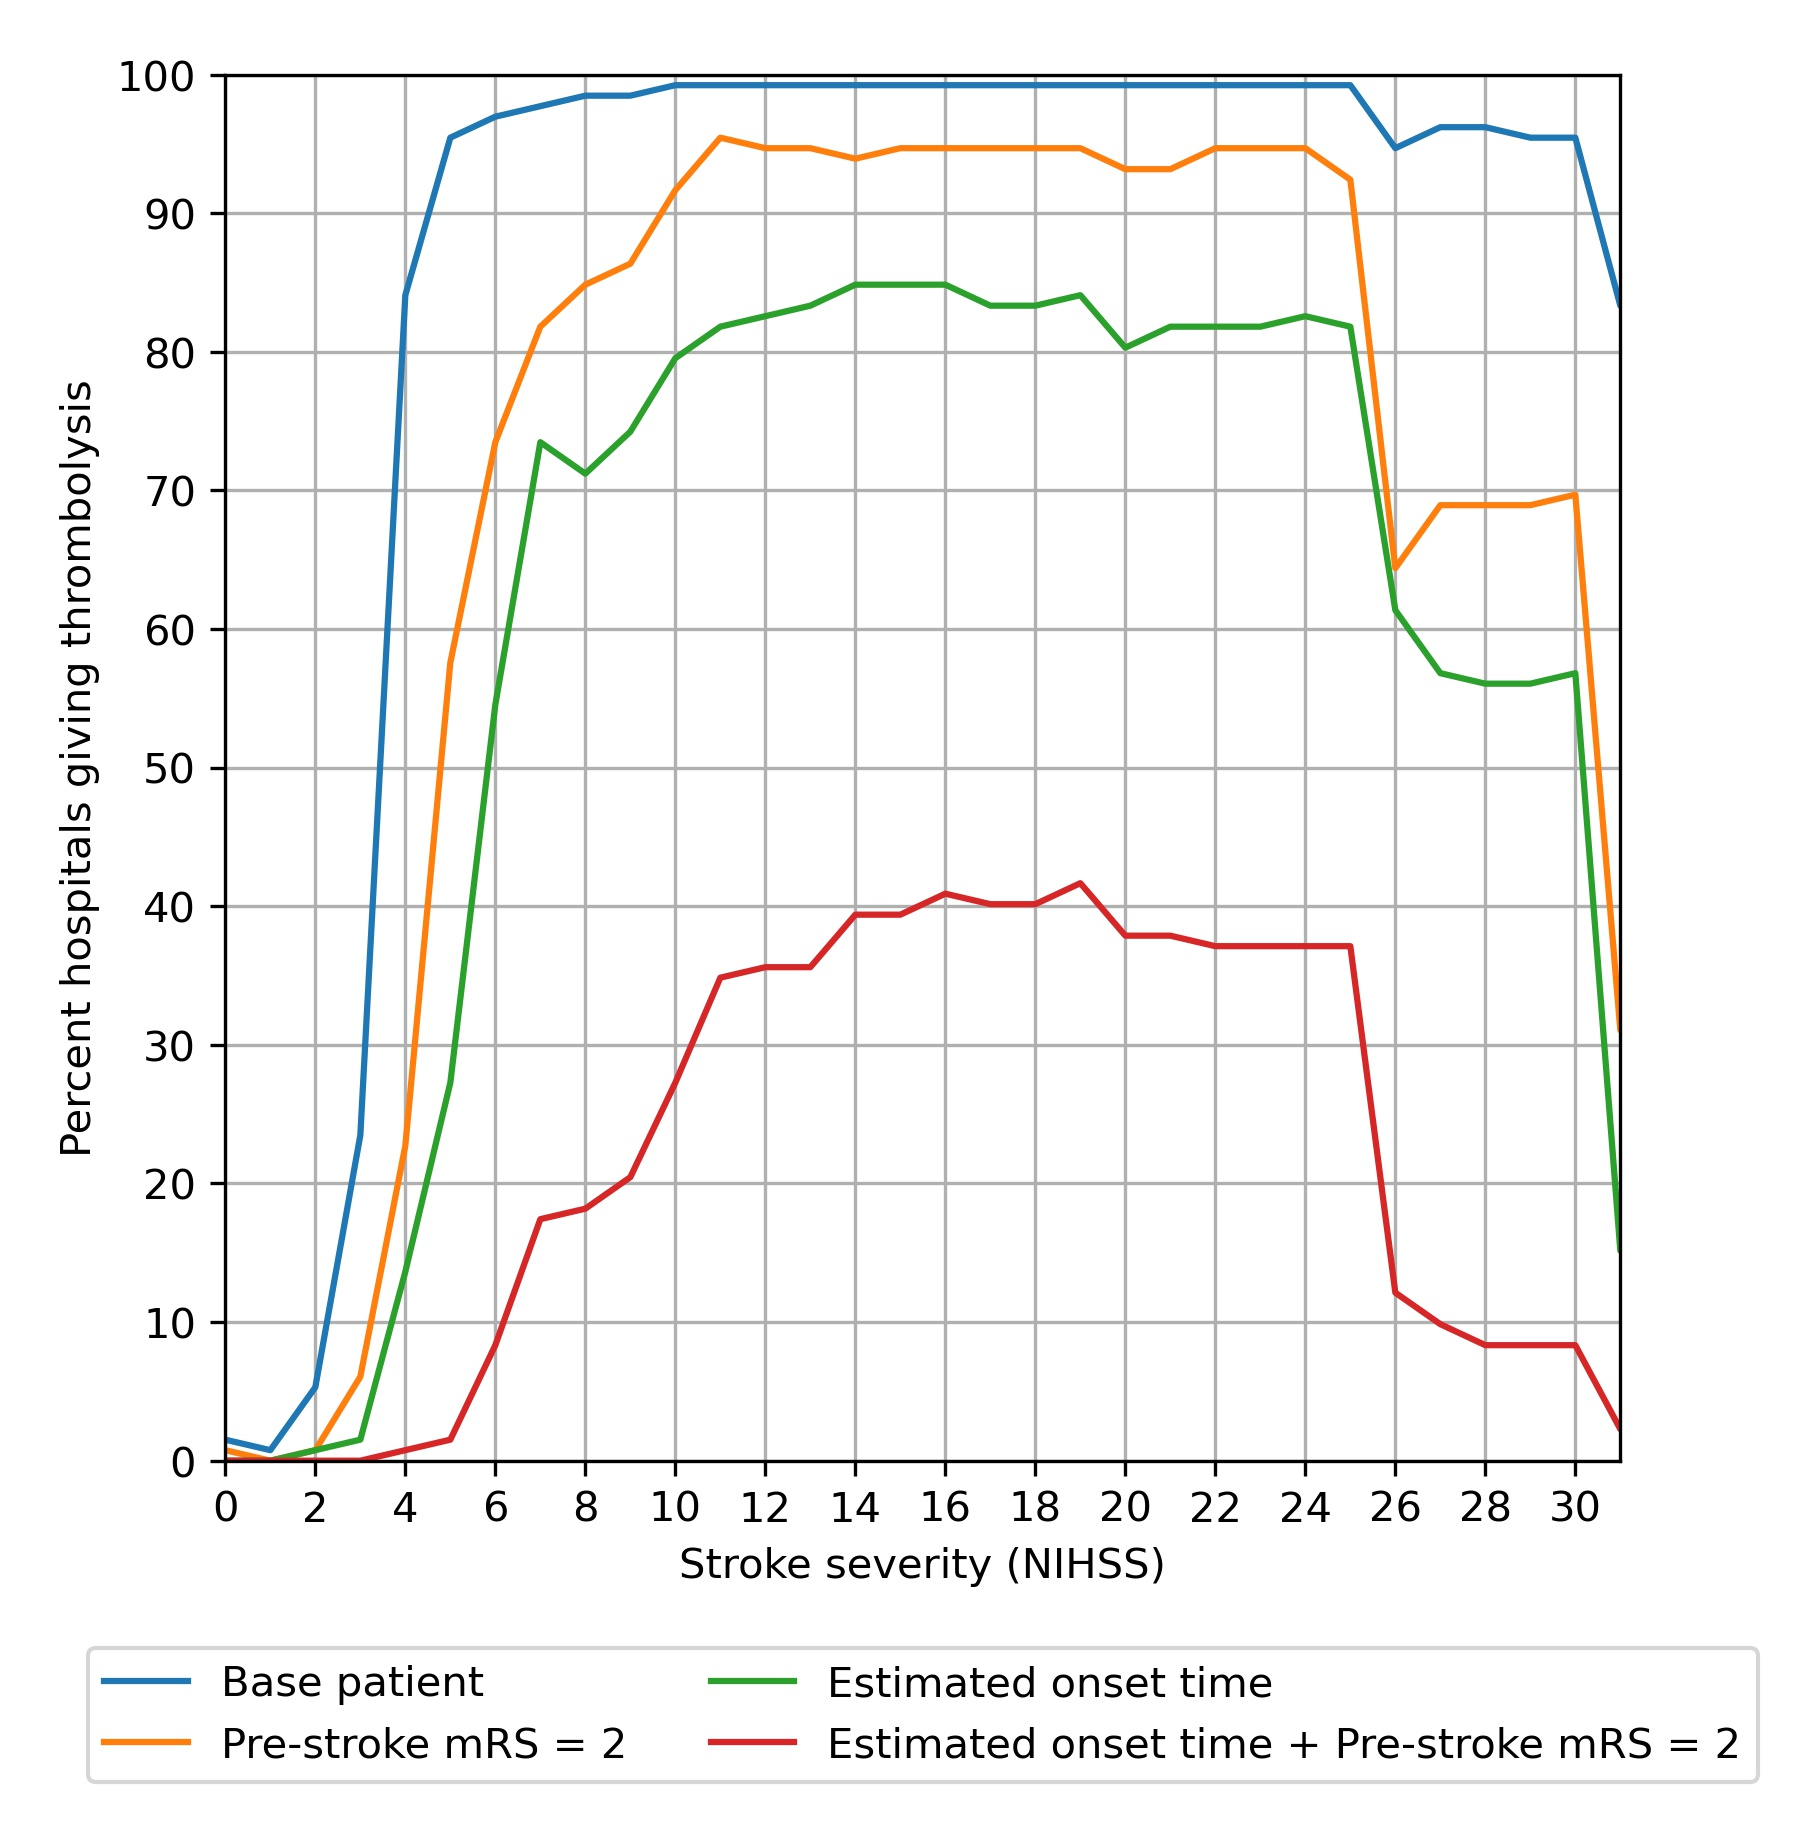
\includegraphics[width=0.8\textwidth]{./images/20_synthetic_xgb_10_features_interactions}
\caption{The effect of changing stroke severity, alone (blue), or coupled with changes to pre-stroke disability (to mRS = 2, orange), precise onset time (to False, green), or changes to both pre-stroke disability and precise onset time (red) on the proportion of hospitals that would be expected to give thrombolysis to a patient. Patients otherwise have the following feature values: Onset to arrival = 80 mins, Arrival to scan = 20 mins, Infarction = 1, NIHSS = 15, Prior disability level = 0, Precise onset time = 1, Use of AF anticoagulants = 0.}
\label{fig:artificial_2}
\end{figure}



%%%%%%%%%%%%%%%%%%%%%%%%%%%%%%%%%%%%%%%%%%%%%%%%%%%%%%%%%%%%%%%%%%%%%%%%%%%%%%%%%%%%%%%

\subsection{10k cohort and \emph{benchmark} decisions}

We investigated, for each hospital, the expected use of thrombolysis for a 10k cohort of patients (the model was trained on the remaining 78,792 patients.

The 30 hospitals with the highest predicted thrombolysis use in the 10k cohort were considered \emph{benchmark} hospitals.

We then took each hospitals own patients and predicted the thrombolysis decision that would made for each patient at each of the hospitals, taking a majority vote of those benchmark hospitals as the \emph{benchmark decision} for that patient. We estimated the use of thrombolysis at each hospital if the benchmark decision was followed for all patients attending each hospital (figure \ref{fig:benchmark}).

83.3\% decisions are identical between local and benchmark decisions. Thrombolysis use would be increased 31.2\% at non-benchmark hospitals if benchmark decisions were made at those hospitals. Overall, thrombolysis use, including at the benchmark hospitals, would be increased 20.7\%. Thrombolysis at the 30 lowest thrombolysing units (judged by expected 10k thrombolysis rate) would be increased 60.2%.


\begin{figure}
\centering
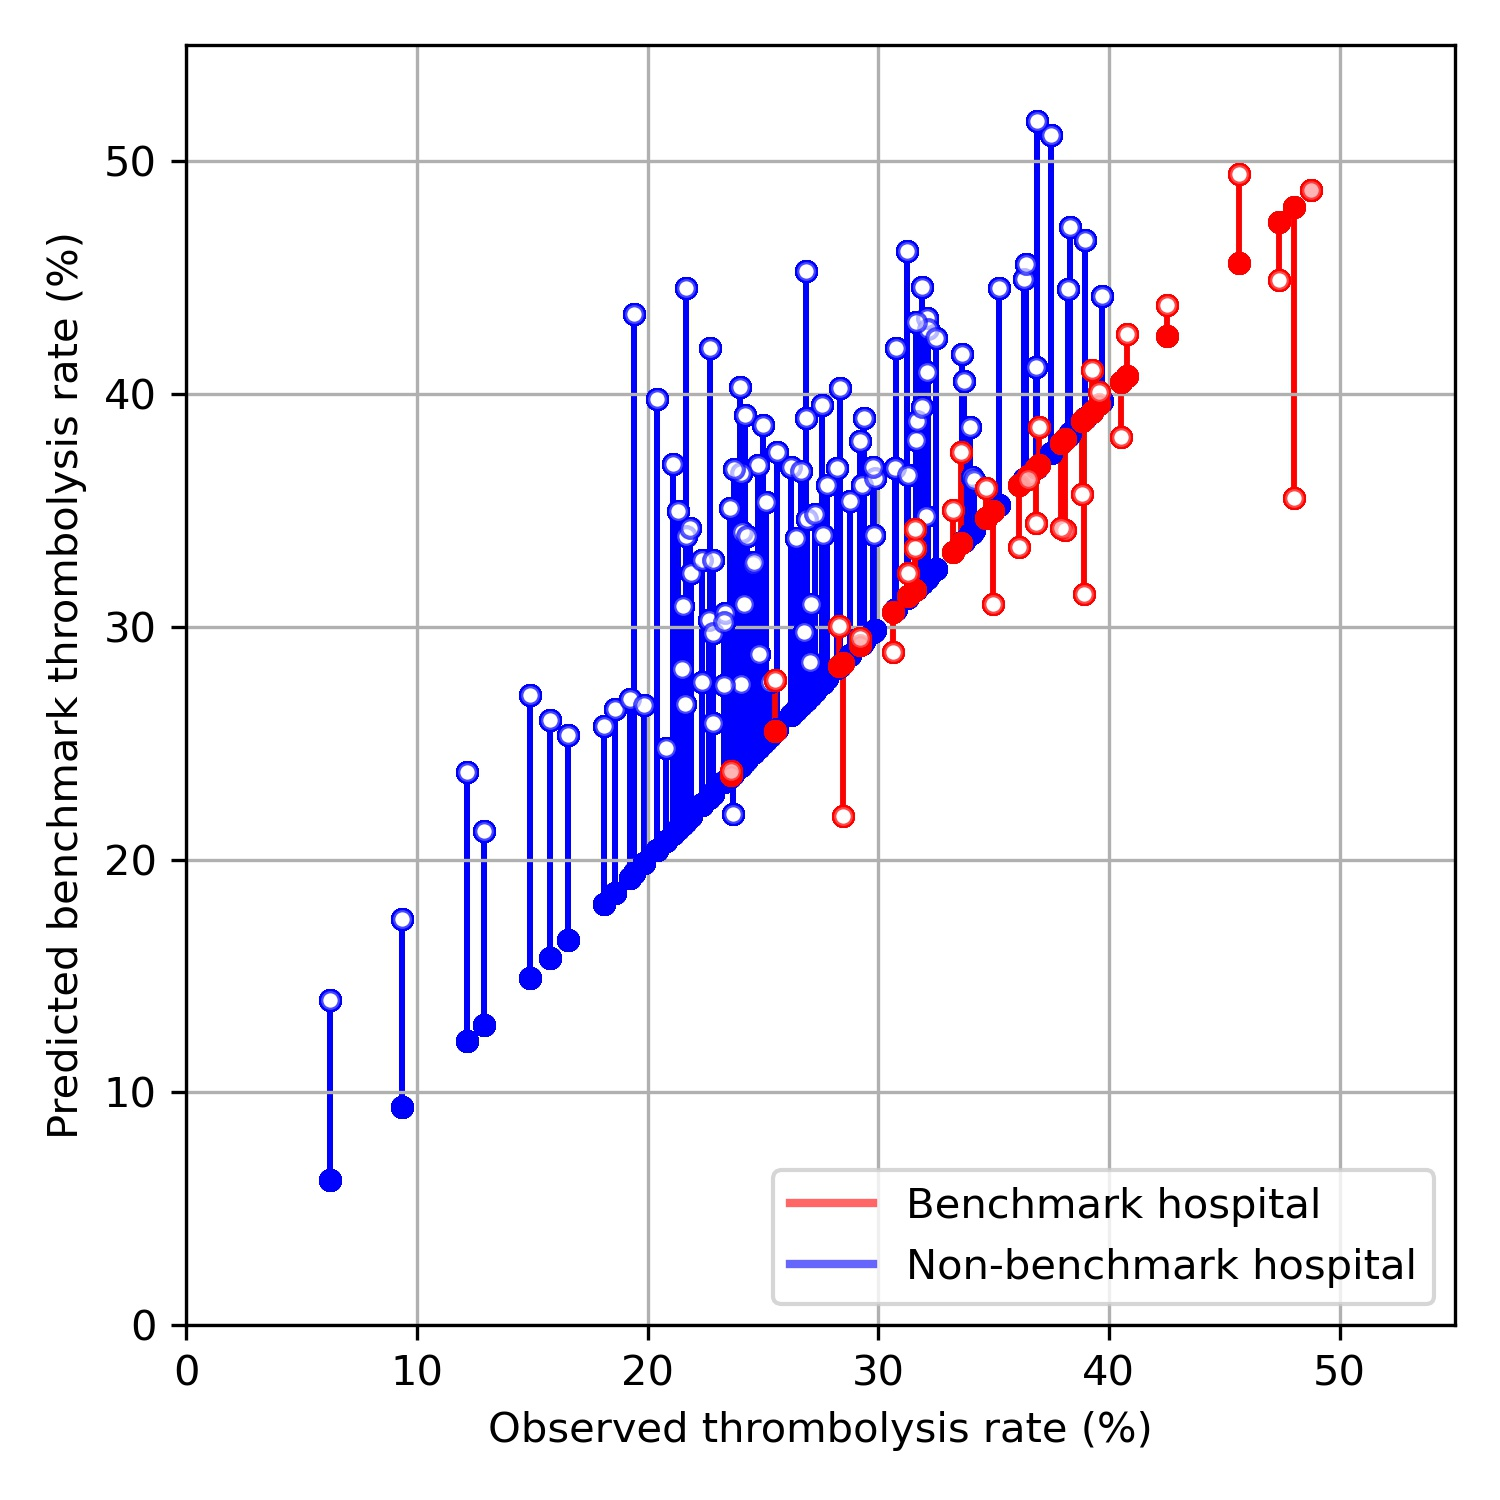
\includegraphics[width=0.7\textwidth]{./images/05_benchmark_thrombolysis_key_features}
\caption{A comparison of observed (actual) thrombolysis rate at each hospital and the predicted thrombolysis rate if decisions were made according to the majority vote of the 30 benchmark hospitals. The solid circle shows the current thrombolysis use, and the open circle shows the thrombolysis use predicted by a majority vote of the benchmark hospitals. The red points are those hospitals that are in the top 30 thrombolysing hospitals (the benchmark set) when 10k cohort thrombolysis use is predicted, with all other hospitals coloured blue.}
\label{fig:benchmark}
\end{figure}


%%%%%%%%%%%%%%%%%%%%%%%%%%%%%%%%%%%%%%%%%%%%%%%%%%%%%%%%%%%%%%%%%%%%%%%%%%%%%%%%%%%%%%%

\subsubsection{Agreement between hospitals on 10k cohort thrombolysis decisions}

We investigated the level of agreement between hospitals in the predicted treatment of the 10k cohort (figure \ref{fig:10k_agreement}. 87.4\% of patients have 80\% of hospitals agree on treatment. For those patients that did actually receive thrombolysis, 78.8\% of patients have 80\% of hospitals agree to thrombolyse. For those patients that did not actually receive thrombolysis, 91.1\% of patients have 80% of hospitals agree not to thrombolyse. 

\begin{figure}
\centering
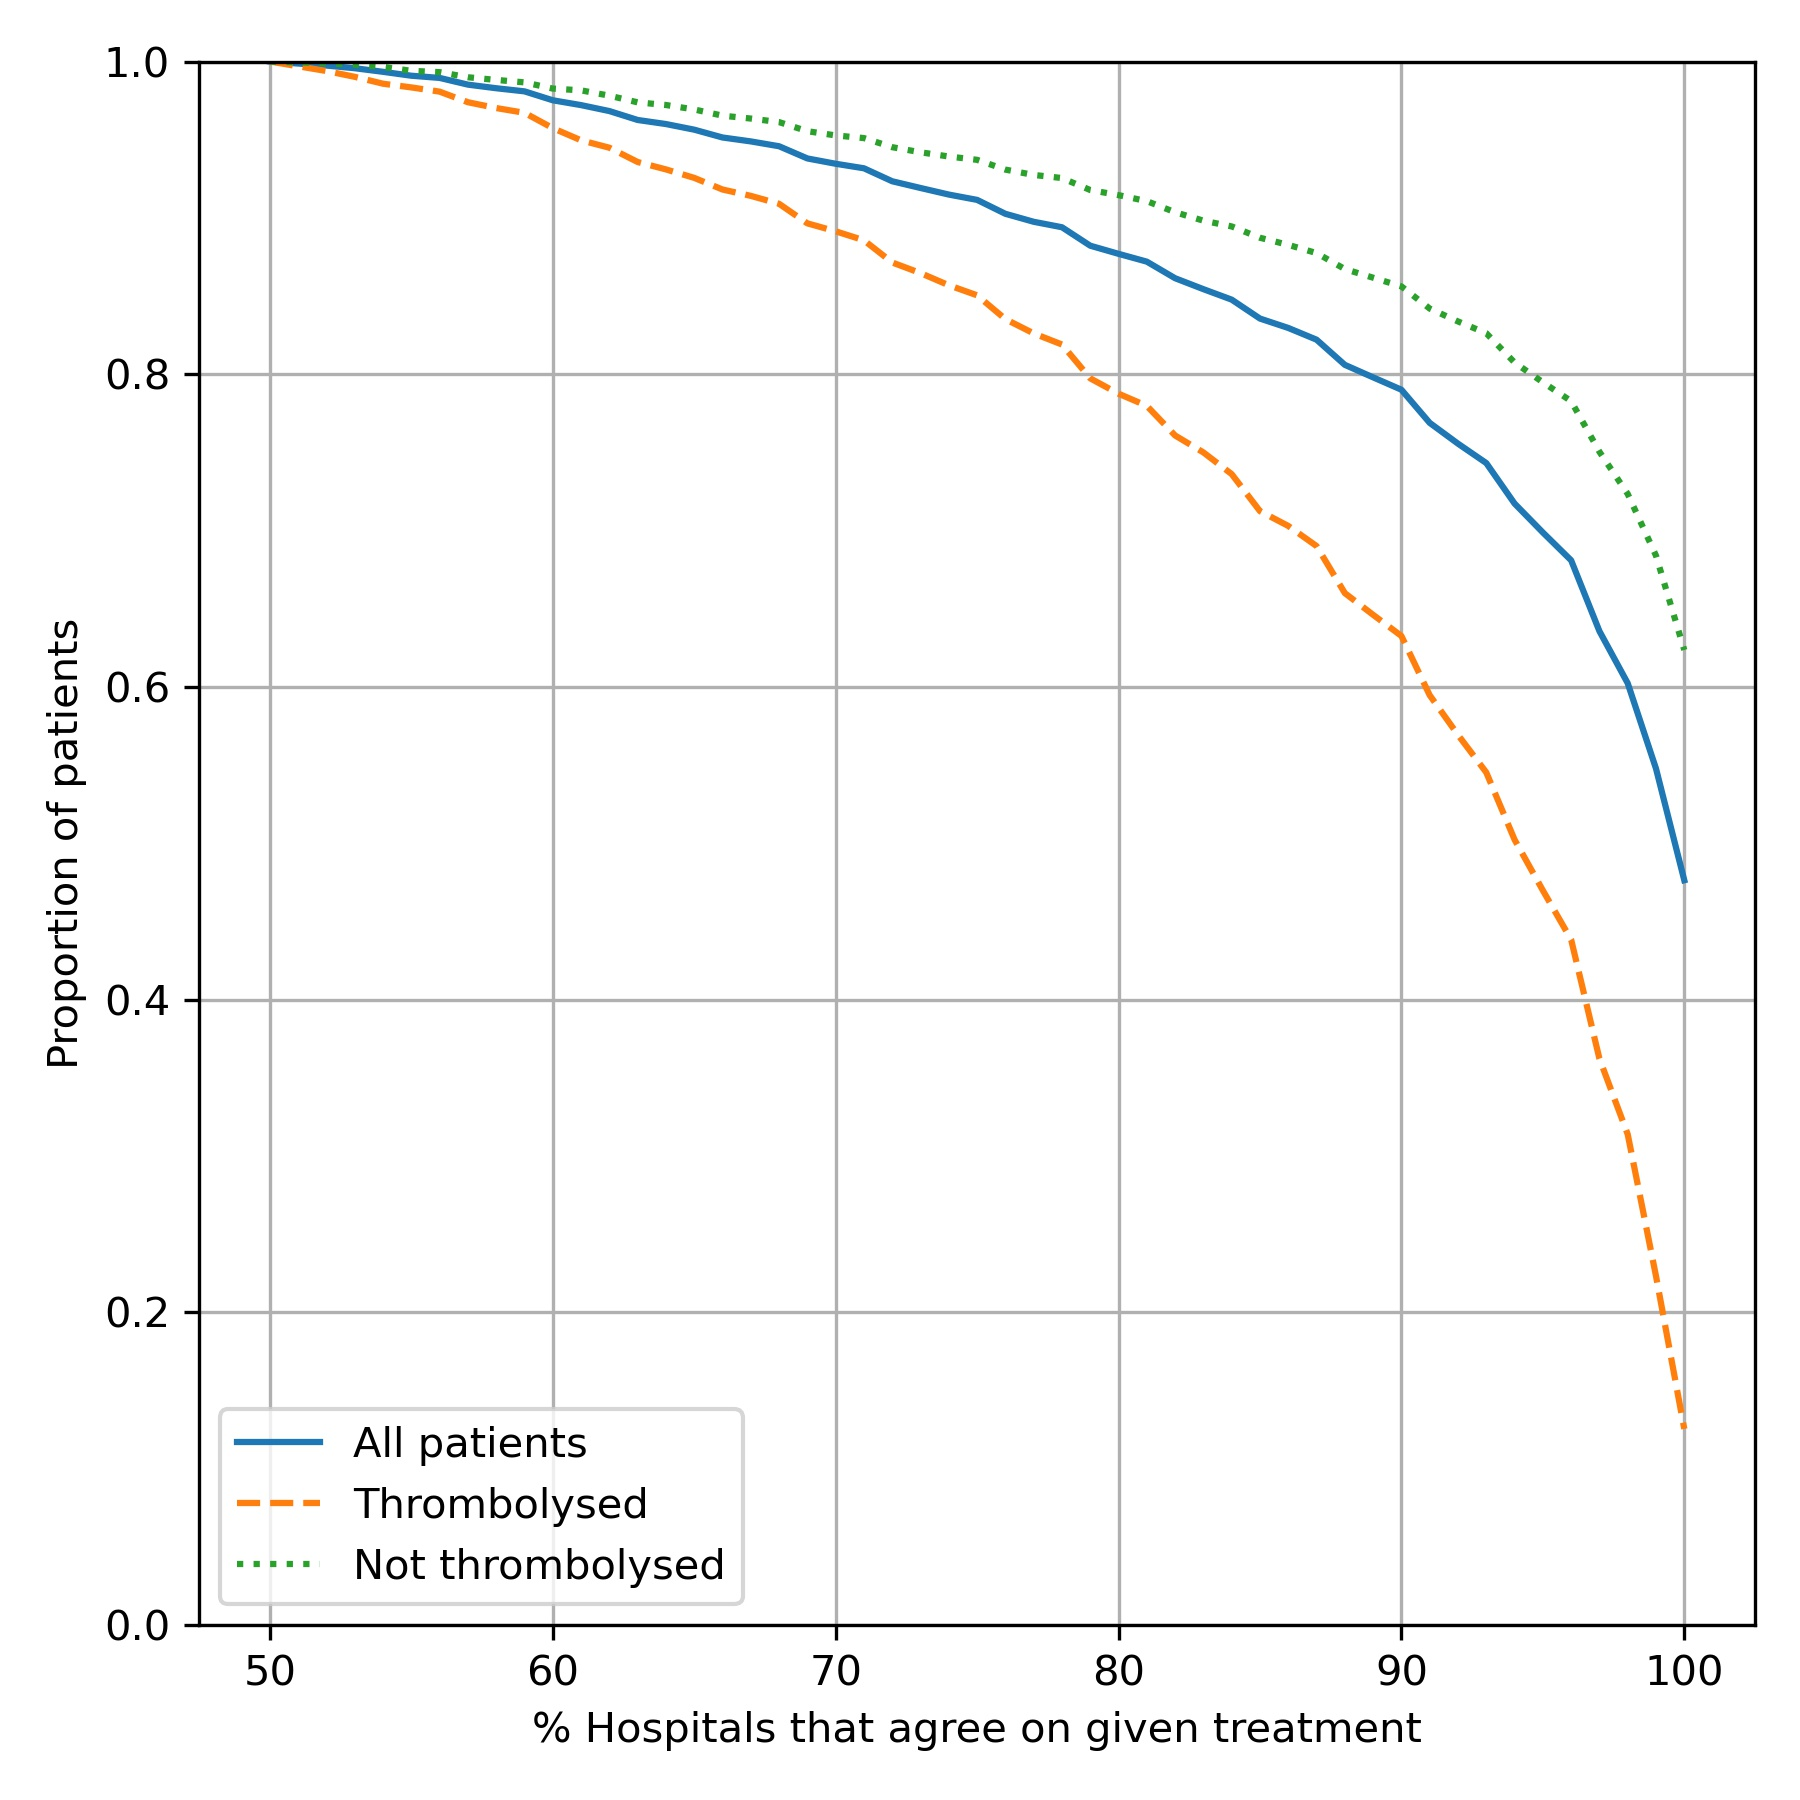
\includegraphics[width=0.7\textwidth]{./images/04_xgb_10_features_10k_cohort_agreement_vs_hospital_single}
\caption{Agreement on decision-making between hospitals when predicting thrombolysis use in the 10k patient cohort. The x-axis shows the proportion of hospitals which must agree on a decision, and the y-axis shows the proportion of patients that have that level of agreement. Analysis is for all decisions (blue solid), for those who did receive thrombolysis (orange dashed), or for those that did not receive thrombolysis (green dotted).}
\label{fig:10k_agreement}
\end{figure}
\fi

\end{document}